\documentclass[trimframe,compontinhos,showtrims,11.5pt,conselho,spreadimages]{memoir}

\usepackage[Kalinka]{hedraoptions} %% << %%%%%%%%%%%%%%%%
\usepackage[baruch]{hedrastyles}
\usepackage[xetex,chicagofootnotes]{tipografia}
\usepackage[standart,sempontinhos]{toc}
\usepackage{hedraextra}
\usepackage{penalidades}
\usepackage{graficos}
\usepackage{hedralogo}
\usepackage{hifensextras}
\usepackage{fichatecnica}
\usepackage{tocloft}
\usepackage[standart]{aparatos}
\usepackage{tabelas}
\usepackage{versos}
\usepackage{gitrevisioninfo}
\usepackage{epigraph}

\usepackage{graphicx}
\usepackage{fancyhdr}
\pagestyle{fancy}
\fancyhf{}
\fancyfoot[LE,RO]{\thepage}
\renewcommand{\headrulewidth}{0pt}

\fancypagestyle{chapter}{
\fancyhf{}
\fancyfoot[RO]{\thepage}
\renewcommand{\headrulewidth}{0pt}
\renewcommand{\footrulewidth}{0pt}}

\usepackage{afterpage}

\newcommand\blankpage{%
    \null
    \thispagestyle{empty}%
    \addtocounter{page}{-1}%
    \newpage}

\usepackage{titlesec}
\titleformat{\part}
[display]
{\Huge\bfseries\BebasNeue}
 {\huge\parttitlename\space\thepart}
  {20pt}
  {\centering\thispagestyle{empty}}


\titleformat{\chapter}
[display]
{\Large\bfseries\MyriadPro}
 {\large\chaptertitlename\space\thechapter}
  {20pt}
  {\centering}

\usepackage{footmisc}

\renewcommand*\footnoterule{}


%\usepackage[utf8]{inputenc}
\usepackage{MyriadPro}
%\setsansfont{MyriadPro}
%\renewcommand{\familydefault}{\sfdefault}
%\DeclareTextFontCommand{\textmyfont}{MyriadPro}
\newfontfamily\MyriadPro[Ligatures=TeX]{MyriadPro-Light}	
\newfontfamily\BebasNeue[Ligatures=TeX]{BebasNeue-Regular}	
\newfontfamily\MinionPro[Ligatures=TeX]{MinionPro-Regular}	

%\setmainfont{MyriadPro-Regular.otf}
\usepackage{fontspec}
\setmainfont[Ligatures=TeX]{Adobe Devanagari}


\usepackage{endnotes}
\renewcommand{\notesname}{Notas}

\counterwithin*{endnote}{part}
\counterwithin*{endnote}{chapter}

\let\latexchapter\chapter
\makeatletter
\renewcommand\enoteheading{%
  \setcounter{secnumdepth}{-2}
  \latexchapter*{\notesname\markboth{NOTAS}{}}
  \mbox{}\par\vskip-\baselineskip
  \let\@afterindentfalse\@afterindenttrue
}
\makeatother


\usepackage{xparse}


\let\latexchapter\chapter

\RenewDocumentCommand{\chapter}{som}{%
  \IfBooleanTF{#1}
    {\latexchapter*{#3}}
    {\IfNoValueTF{#2}
       {\latexchapter{#3}}
       {\latexchapter[#2]{#3}}%
     \addtoendnotes{\unexpanded{\enotedivision{\subsection}{#3}}}
    }
}
\makeatletter
\def\enotedivision#1#2{\@ifnextchar\enotedivision{}{#1{#2}}}
\makeatletter

%\linespread{1.08}
\usepackage{commands}

\usepackage{setspace}

\usepackage{multirow}

\makeatletter
\newenvironment{Parskip}{%
   \par
   \parskip=0.3\baselineskip \advance\parskip by 0pt plus 2pt
   \parindent=\z@
   \def\@listI{\leftmargin\leftmargini
      \topsep\z@ \parsep\parskip \itemsep\z@}
   \let\@listi\@listI
   \@listi
   \def\@listii{\leftmargin\leftmarginii
      \labelwidth\leftmarginii\advance\labelwidth-\labelsep
      \topsep\z@ \parsep\parskip \itemsep\z@}
   \def\@listiii{\leftmargin\leftmarginiii
       \labelwidth\leftmarginiii\advance\labelwidth-\labelsep
       \topsep\z@ \parsep\parskip \itemsep\z@}
   \partopsep=\z@
}{\par}
\makeatother

\makeatletter
\newenvironment{myParskip}{%
   \par
   \parskip=0.2\baselineskip \advance\parskip by 0pt plus 2pt
   \parindent=\z@
   \def\@listI{\leftmargin\leftmargini
      \topsep\z@ \parsep\parskip \itemsep\z@}
   \let\@listi\@listI
   \@listi
   \def\@listii{\leftmargin\leftmarginii
      \labelwidth\leftmarginii\advance\labelwidth-\labelsep
      \topsep\z@ \parsep\parskip \itemsep\z@}
   \def\@listiii{\leftmargin\leftmarginiii
       \labelwidth\leftmarginiii\advance\labelwidth-\labelsep
       \topsep\z@ \parsep\parskip \itemsep\z@}
   \partopsep=\z@
}{\par}
\makeatother

\newcommand{\mystar}{{\fontfamily{lmr}\selectfont$\star$}}

%\makeatletter
%\renewcommand{\@chapapp}{}% Not necessary...
%\newenvironment{chapquote}[2][2em]
%  {\setlength{\@tempdima}{#1}%
%   \def\chapquote@author{#2}%
%   \parshape 1 \@tempdima \dimexpr\textwidth-2\@tempdima\relax%
%   \itshape}
%  {\par\scriptsize\hfill-- \chapquote@author\hspace*{\@tempdima}\par\bigskip}
%\makeatother

%\newcommand\Chapter[2]{\chapter
%  [#1\hfil\hbox{}\protect\linebreak{\itshape#1}]%
%  {#1\\[2ex]\Large\itshape#2}%
%}

%\usepackage{graphicx,eso-pic,etoolbox}
%\providecommand{\parthook}{}
%\patchcmd{\part}{\thispagestyle}{\parthook\thispagestyle}{}{}
%\newcommand{\partimage}[2][]{% \parthook[<options>]{<image>}
%  \renewcommand{\parthook}{% Update \parthook
%    \AddToShipoutPictureBG*{% Add picture to background of THIS page only
%      \AtPageLowerLeft{\includegraphics[width=\paperwidth,height=\paperheight,#1]{#2}}}% Insert image
%    \renewcommand{\parthook}{}}}% Restore \parthook

\begin{document}

%!TEX root=./LIVRO.tex

%\chapter*{Prefácio\\
\bigskip
\emph{A crítica deve brotar de uma dívida de amor}}

\addcontentsline{toc}{part}{Prefácio}

\hedramarkboth{Prefácio}{}


Com a afirmação que intitula este prefácio George Steiner abre o seu primeiro livro de crítica
literária, de 1959, intitulado \emph{Tolstói ou Dostoiévski -- Um ensaio
sobre o velho criticismo}.\footnote{\scalebox{0.8}{STEINER}, G. \emph{Tolstói ou
  Dostoiévski -- um ensaio sobre o velho criticismo}. São Paulo:
  Perspectiva, 2017.} Através de algum instinto primário de comunhão,
pondera o crítico, buscamos passar aos outros a qualidade e a força de
nossa experiência. ``Gostaríamos de persuadi"-los a se abrirem para ela.
Dessa tentativa de persuasão se originam as intuições mais verdadeiras
da crítica'' (\scalebox{0.8}{STEINER},~2017,~p.~1).

Estas \emph{Aulas de literatura russa}, de autoria de Aurora Fornoni
Bernardini, constituem, certamente, o fruto de suas intuições mais
verdadeiras, surgidas e acumuladas no decorrer de vários anos no
exercício ininterrupto da pesquisa acadêmica, da crítica literária e da
docência no campo dos estudos russos.

Na verdade, esta coletânea de ensaios vem preencher entre nós muito
oportunamente uma lacuna editorial: embora a literatura e a cultura
russas vivam hoje no Brasil um de seus momentos mais profícuos de
difusão, a considerar o número cada vez maior de títulos e
autores russos traduzidos para a língua portuguesa e disponíveis nas
livrarias brasileiras, o leitor não dispõe de uma escolha
tão ampla quando se trata de estudos ensaísticos,
produzidos por nossa eslavística e dedicados, em particular, à análise e
à teoria literária.

A presente antologia estruturada em quatro partes (``Obras e
autores'', ``Teóricos'', ``Entrevistas'' e ``Relatos'') constrói um movimento crítico de viés,
em certa medida, historiográfico e cronológico da literatura russa
(especialmente na abordagem dos autores da primeira parte),
sem prejuízo algum da verticalidade que marca as análises de obras literárias, de fatos artísticos, filosóficos,
sociológicos, linguísticos, culturais e históricos, embasadas em agudo
senso de pesquisa e ensino acadêmicos.

Não sem razão: Aurora Fornoni Bernardini é professora, ensaísta,
escritora, tradutora e artista plástica e tem papel relevante na
tradição dos estudos e da tradução literária de
textos russos no Brasil. Na Universidade de São Paulo criou nos anos
1960, juntamente com Boris Schnaiderman, um núcleo de ensino e pesquisa,
ainda em plena expansão, que se tornou referência na divulgação das
primeiras traduções diretas de obras russas não apenas de titãs da prosa e da
poesia, mas também de teóricos que alimentaram, e até hoje
alimentam, estudiosos da literatura e da teoria literária (e não apenas
a russa).

Basta citar alguns dos muitos autores traduzidos por Aurora Bernardini
no âmbito teórico e literário --- Tchékhov, Akhmátova, Tyniánov,
Meletínski, Bakhtin, Eisenstein, Tsvetáieva, Bábel,
Khlébnikov, Turguêniev, Ivanóv, Mandelstam, Sologub\ldots{} --- para se ter uma
ideia do largo espectro de seus interesses intelectuais e de sua
contribuição para o alargamento do horizonte cultural de
nosso país. A lista seria ainda maior se a ela acrescentássemos os autores
e títulos italianos e ingleses a que o público brasileiro teve acesso
por meio de suas traduções.

Numa época em que a especialização crescente grassa no ambiente acadêmico, as atividades de crítica e de criação de Aurora
Bernardini e, sobretudo, as suas preocupações pedagógicas e de formação
vêm demonstrar o alcance de seu pensamento e da missão de seu ofício
como docente e intelectual.

Prova disso encontramos nessas \emph{Aulas de literatura russa} --- o título
não poderia ser mais adequado.

O conjunto de textos aqui reunidos configura menos uma antologia de
ensaios esparsos, e mais, isto sim, uma obra à qual não faltam unidade
e organicidade, posto que resultado de apurada reflexão, amparada por
sólido aparato teórico"-crítico e nutrida por inúmeras aulas, artigos, palestras, resenhas
e diferentes publicações, trabalhos cuja pertinência e importância para os estudos russos podem
ser agora melhor aferidas numa leitura integrada.

Nesse sentido, a segunda parte do livro, dedicada a estudos teóricos,
conforma, por assim dizer, algumas chaves metodológicas e
elucidativas que dialogam subliminarmente com os textos que
estruturam a primeira parte. Esse diálogo crítico"-teórico entre
os ensaios do livro propicia uma espécie de ressonância estética e
histórico"-cultural entre os autores e textos analisados, e
encaminha, afinal, uma apreensão dos elos explícitos ou implícitos que
impulsionam o desenvolvimento da literatura e da cultura russas ao longo do
tempo.

As ``aulas'' constantes da primeira parte do volume --- dedicadas a
Púchkin, Gógol, Gontcharóv, Turguêniev, Dostoiévski, Tolstói, Tchékhov,
Búnin, Górki, Maiakóvski, Tsvetáieva, Kharms, Bródski, Nabókov\ldots{} e a outros nomes"-chaves da
história literária e cultural russa, desde a sua formação até os dias de
hoje --- empreendem recortes analíticos argutos e originais, balizados pela busca de uma leitura imanente do
texto literário, sem desdenhar, porém, um olhar crítico transversal para
a captação de aspectos biográficos, filosóficos, políticos, sociais ou
ideológicos da criação artística.

Tal \emph{modus operandi} se alicerça, certamente, na autoridade de quem
acompanhou a introdução das teorias do formalismo russo no ambiente
intelectual brasileiro. No ensaio intitulado ``Formalismo
russo, uma revisão e uma atualização'', a autora discorre sobre as
inflexões desse movimento na teoria literária contemporânea,
tema de uma alentada pesquisa realizada nos idos de 1990. Ao
passar a limpo nomes seminais da teoria literária russa, como Iúri
Tyniánov, Roman Jakobson, Víktor Chklóvski, Óssip Brik, Boris Tomachévski,
Boris Eikhenbaum, Vladímir Propp e outros, Aurora Bernardini ressalta a
vigência de conceituações essenciais do formalismo russo, capazes de
responder a questões que cercam a pós"-modernidade: ``O que é
literatura?'', ``O que diferencia a literatura de outros domínios da
escrita?'', ``Como se estrutura o mundo do texto frente ao mundo de que
ele é imagem?''.

O conceito de \emph{dominante} como princípio organizador do texto; as
funções da linguagem; a equivalência em poesia de dois
eixos, o paradigmático (metafórico) e o da contiguidade (metonímico); o
conceito de \emph{estranhamento}; a questão da determinação da ``diferença
específica'', do traço distintivo, do critério qualitativo que permite estabelecer os limites da literatura frente às outras
expressões das Humanidades; enfim, a análise dos procedimentos que
implicam, afinal, o conceito de \emph{literaturnost} (\emph{literariedade}), caro
aos formalistas russos, está posta aqui sob exame para atestar
a permanência dessas teorias e sua eficácia na abordagem do fato
literário e artístico.

Exemplo disso, e da já mencionada simbiose teórico"-crítica entre as duas
primeiras partes do livro, são as análises das poéticas de Khlébnikov, Tsvetáieva,
Kharms e Bródski apresentadas nas seções ``Vanguardas e modernismo'' e ``Contemporâneos (século \scalebox{0.8}{XX})''. Os
poetas e seus respectivos poemas são perscrutados, mesmo que de modo
oblíquo, à luz de muitas das considerações do formalismo russo. Dessa maneira, a
concepção da linguagem poética como discurso autônomo e como uma
dinâmica semântica específica aparece explicitada na práxis analítica da ensaísta.

Ao rebater com veemência a apreensão distorcida de certa crítica
detratora do formalismo russo, movida por um
conhecimento muitas vezes ``superficial, textos copilados e mal
traduzidos'', Aurora Bernardini nos oferece no referido ensaio um amplo painel desse movimento
russo --- desde seus precursores, seu surgimento e desenvolvimento, até o
legado para a crítica e a teoria literária contemporâneas. Iluminam"-se,
assim, os eixos principais por meio dos quais os formalistas
puderam compreender a obra literária como um ``dinamismo interno'' de
determinado sistema, com suas leis imanentes, inserindo"-a, ao mesmo
tempo, nas diferentes séries sociais e históricas, aspecto este pouco
relevado por uma crítica mais apressada, mas sublinhado neste volume.

Há que se ressaltar que a lucidez crítica esboçada aqui
afunda raízes em três importantes trabalhos acadêmicos
escritos pela autora em diferentes momentos de sua trajetória crítica:
\emph{Materiais para o estudo do futurismo italiano e do futurismo russo}
(1970), \emph{Poéticas do futurismo russo e italiano} (1973) e
\emph{Indícios flutuantes em Marina Tsvetáieva} (1977).

Desse debate sobre o formalismo russo e a
contemporaneidade participa ninguém menos do que Victor Erlich, autor de
um dos mais importantes estudos sobre o tema,\footnote{\scalebox{0.8}{ERLICH}, Victor. \emph{Russian
 formalism: History -- Doctrine.} New Haven: Yale University Press,
 1981, 3ª ed.} a quem a autora recorre por ocasião de uma visita
a Yale, deixando registrada na instigante entrevista publicada nesta
coletânea (``Reverberações do formalismo russo na crítica literária 
americana'') a profética asserção do eminente estudioso, discípulo de Roman
Jakobson: ``após o formalismo russo nada de mais original ou importante
teria surgido no domínio da Teoria da Literatura''.

Aliás, a estratégia crítica de dar viva voz a especialistas renomados
para a discussão de temas, autores e obras específicas se mostra
produtiva em outra entrevista aqui incluída. O diálogo com Joseph Frank,
um dos maiores conhecedores da vida e obra de F. Dostoiévski, vem
esclarecer não apenas questões atinentes ao contexto estético,
ideológico e religioso a que o romancista russo reage por meio de sua
obra, mas também vieses da crítica dostoievskiana, como as teorias de
Bakhtin, por exemplo.

Corrobora esse incessante movimento de interlocução crítica presente na
coletânea outra vertente analítica: a literatura comparada. O
ensaio ``Encontro de andarilhos'', entre Velimir Khlébnikov e Manoel
de Barros, propõe imersões comparativas desafiadoras entre universos
artísticos e culturais, \emph{a priori}, dessemelhantes. Mas a crítica
comparada se insinua também em ``Dostoiévski e Púchkin'' e ``Tolstói e
Dostoiévski'', numa espécie de interação russa
``intramuros''.

Desta recolha de textos de Aurora Bernardini, sob organização de dois de
seus discípulos, depreende"-se, afinal, um dos axiomas fundamentais dos
estudos literários --- a concepção da crítica literária não
apenas como uma espécie de apêndice superficial da literatura, mas,
conforme salienta Todorov, como seu duplo necessário, porque um texto
artístico talvez nunca possa dizer a totalidade da sua verdade: ele não
deve significar, mas simplesmente ser uma nova luz lançada sobre o
mundo.

Concluem esse amplo percurso crítico a seção de entrevistas com a
 autora e a de relatos. Além de um valioso testemunho sobre a 
trajetória intelectual do professor, ensaísta e tradudor Boris 
Schnaiderman, a escritora nos apresenta uma inesperada e subjetiva nota
``sentimental''. ``Minha última viagem sentimental à \scalebox{0.8}{URSS}'' é um relato
de viagem colorido por impressões e recordações pessoais que evocam um
tempo vivido numa Rússia pretérita presentificado na
memória do observador. Permanecem o mesmo olhar e o mesmo rigor
inquiridores na sondagem de uma cultura e de uma história às quais uma
vida inteira está dedicada. Mas, agora, nessa escrita do eu a crítica se
reveste de criação, e a dívida de amor parece brotar dessas derradeiras
linhas\ldots{}

As páginas que se seguem são um convite ao leitor para perfazer essa
bela aventura do espírito.

\begin{flushright}
\emph{Arlete Orlando Cavaliere}
\end{flushright}



%\textbf{AULAS DE LITERATURA RUSSA: DE PÚCHKIN A GORENSTEIN}%

%\textbf{Í N D I C E}%

%\textbf{I. Estdos sobre autores}%

%1.1 Púchkin e o começo da literatura russa -- \textbf{pp. 03-05}%

%1.2 Púchkin: algumas considerações -- \textbf{pp. 05-07}%

%1.3 Evguêni Onéguin -- \textbf{pp. 7-11}%

%1.4 Gógol, o pregador do feudalismo -- \textbf{pp. 11-13}%

%1.5 Turguêniev e a \emph{intelligentsia} russa -- \textbf{pp. 13-23}%

%1.6 A longa provação de Dostoiévski -- \textbf{pp. 23-25}%

%1.7 Aurora Bernardini entrevista Joseph Frank: Sobre Dostoiévski --
%\textbf{pp. 25-33}%

%1.8 Dostoiévski e Púchkin -- \textbf{pp.34-41}%

%1.9 Algumas questões fundamentais na vida e na obra de Dostoiévski --
%\textbf{pp. 41-48}%

%1.10 O Grande Inquisidor e \emph{Os Irmãos Karamázov} -- \textbf{pp.
%49-59}%

%1.11 Considerações à margem de Anna Kariênina -- \textbf{pp. 59-70}%

%1.12 As cartilhas do Conde Liev Nikoláievitch Tolstói -- \textbf{pp.
%70-74}%

%1.13 \emph{A morte de Ivan Ilitch} -- Liev Tolstói em quadrinhos --
%\textbf{pp.75-76}%

%1.14 Tolstoismo e hinduísmo -- \textbf{pp. 76-84}%

%1.15 Tolstói e Dosteoiévski -- \textbf{pp. 84-91}%

%1.16 Os escritores russos na época do ppulismo -- \textbf{pp.91-101}%

%1.17 Tchekhov, o interprete do grande tédio russo -- \textbf{pp.
%101-108}%

%1.18 De Tchekhov a Pirandello -- \textbf{pp. 108-117}%

%1.19 O evocador de um mundo primitivo - Sobre Górki \textbf{- pp.
%117-120}%

%1.20 Encontro de andarilhos -- \textbf{pp. 121-137}%

%1.21 Aspectos da natureza em velímir khlébnikov e em manoel de barros --
%\textbf{137 - 147}%

%1.22 Marina Tsvetáieva, poetisa russa: esboço de vida e obra --
%\textbf{pp. 148 - 159}%

%1.23 Prefácio a Bródski -- \textbf{pp. 159-168}%

%1.24 O mundo absurdo de Daniil Kharms -- \textbf{pp. 168-179}%

%1.25 \emph{Parque Cultural} ou Um escritor russo na América: sobre
%Dovlátov -- \textbf{pp.179 -- 181}%

%1.26 Friedrich Gorenstein: \emph{Salmo}- um romance-meditação sobre os
%quatro flagelos do Senhor -- \textbf{pp. 181-184}%

%\textbf{II. Estudos teóricos}%

%2.1 Minha última viagem sentimental à URSS (1989) -- \textbf{pp.
%184-204}%

%2.2 Dos diários de serguéi eisenstein e outros ensaios \textbf{pp.
%204-209}%

%2.3 \emph{Antologia do pensamento crítico russo} (1802-1901) --
%\textbf{pp. 188-191}%

%2.4 Formalismo e poesia -- \textbf{pp. 212-237}%

%2.5 Formalismo russo, uma revisão e uma atualização -- \textbf{pp.
%224-237}%

%2.6 Reverberações do formalismo russo na crítica literária amaricana:
%Aurora Bernardini \textbf{pp. 238-243}%

%2.7 O papel do conflito no conto russo de magia -- \textbf{pp. 243-252}%

%2.8 O orgânico e o patético em S.M. Eisenstein -- \textbf{pp. 251-258}%

%\textbf{PÚCHKIN E O COMEÇO DA LITERATURA RUSSA}\endnote{Originalmente
%  publicado no \emph{Caderno de Literatura e Cultura Russa}, edição de
%  2004. (Número dedicado ao escritor Aleksandr Púchkin)}%

%\textbf{~}

%\begin{longtable}[]{@{}l@{}}
%\toprule
%\endhead
%~\tabularnewline
%\bottomrule
%\end{longtable}

\part{Obras e autores}
\makebox[0pt][l]{%
  \raisebox{-\totalheight}[0pt][0pt]{%
    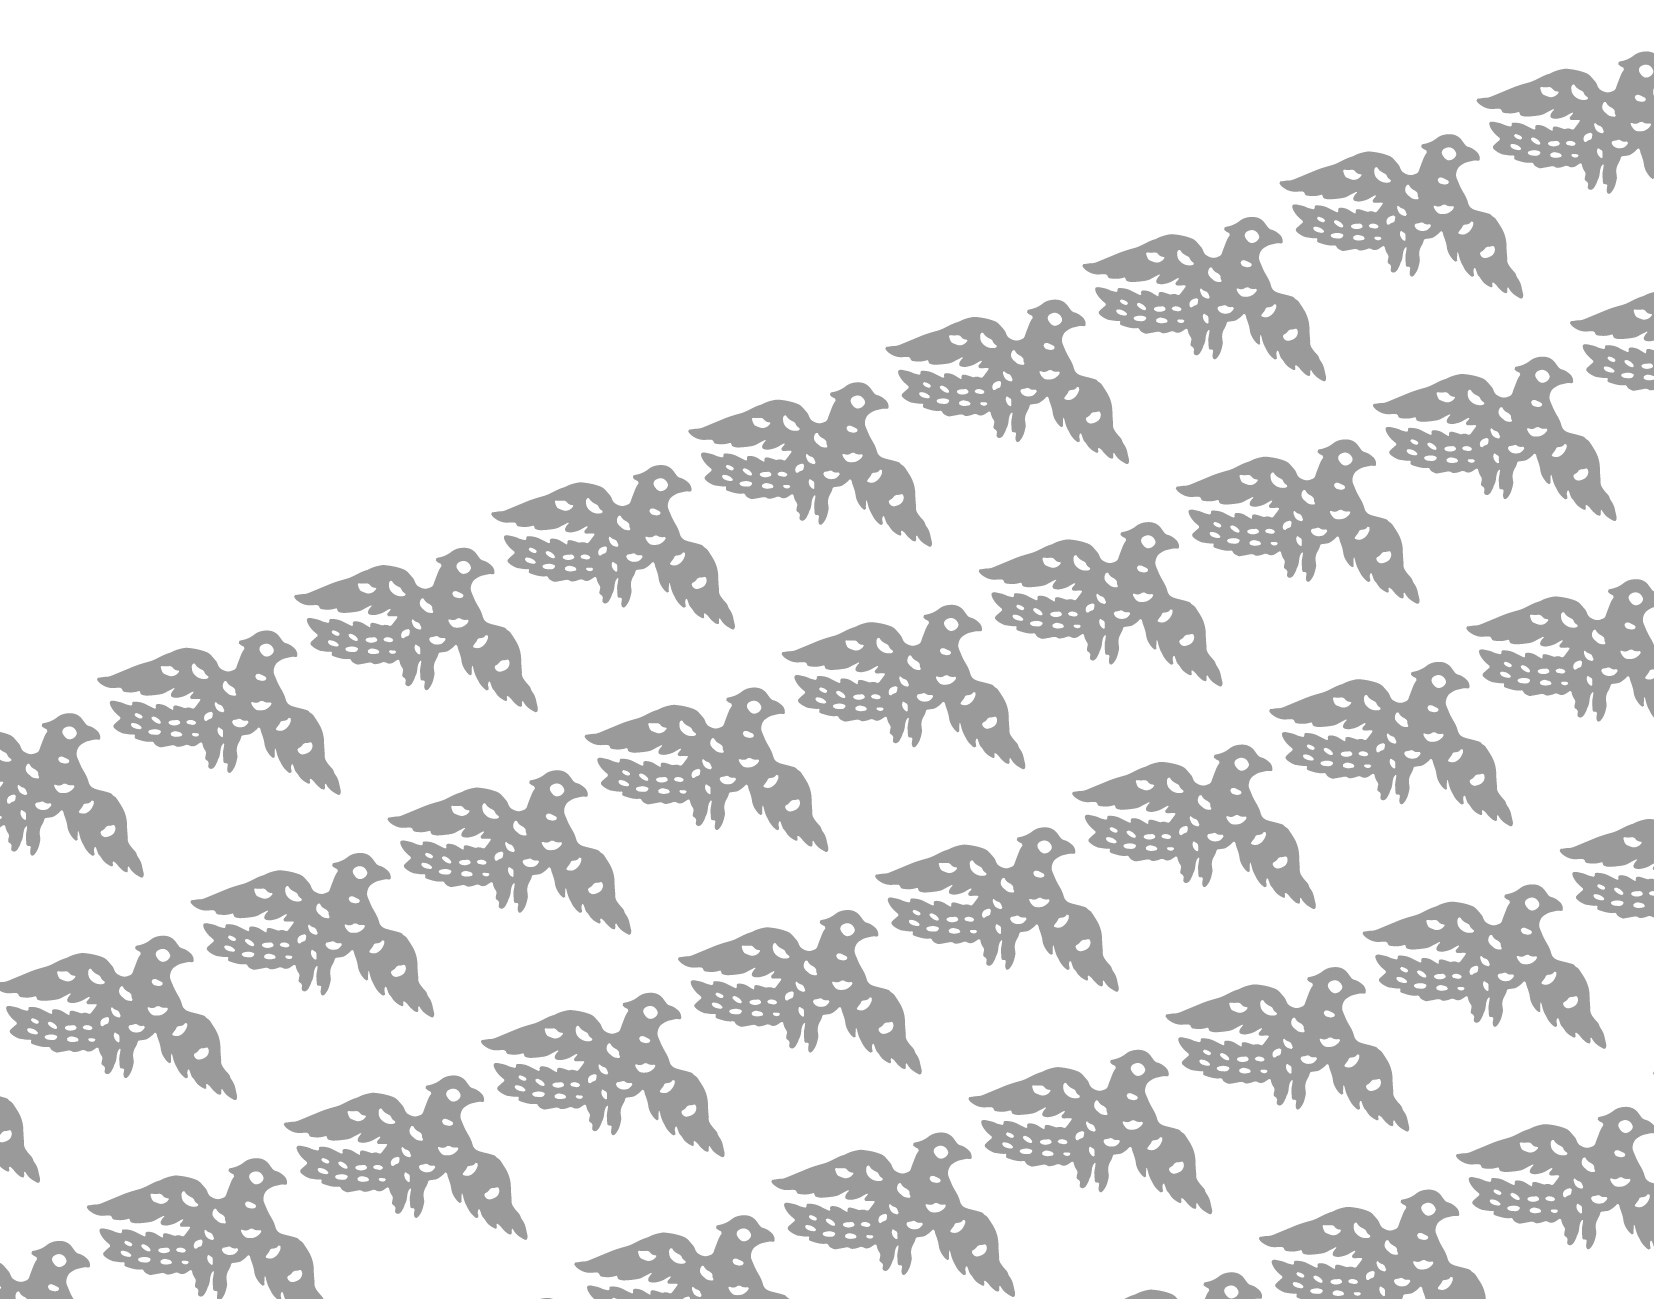
\includegraphics[width=4in]{./imgs/passaro.jpg}}}%
%\part[Foo]{Foo\\[2ex]\makebox[0pt]{\includegraphics[width=166mm]{./img/passaros.jpg}}}
%{Obras e autores\\[2ex]\makebox[0pt]{\includegraphics[width=\paperwidth]{filename}{\paperwidth}{0.25\paperwidth}}}



\part{Romantismo e realismo}

\chapter{Púchkin e o começo da literatura russa\footnote{Publicado no \emph{Caderno de literatura e cultura russa (Dossiê Púchkin)} Organização Homero Freitas de Andrade. São Paulo: Ateliê editorial, 2004, pp.31.--40.}}

Numa admirável introdução a \emph{The Oxford Book of Russian Verses}, \footnote{{\MinionPro{\versal{BARING}}}, Maurice. \emph{The Oxford Book of Russian Verses.} Oxford: Claredon Press, 1958.}
Maurice Baring sintetiza, dentro do panorama da literatura ocidental, o
advento de Aleksandr Serguéievitch Púchkin (1799--1837), explicando por
que ele é considerado por muitos estudiosos o grande iniciador da
literatura russa. É claro que ela não nasceu no século {\MinionPro{\versal{XIX}}}. Porém, durante muito tempo seu curso foi subterrâneo, acompanhando o atormentado
desenrolar da própria história da Rússia.

Já no século {\MinionPro{\versal{XI}}}, após a consolidação da unificação das tribos eslavas,
Kiev, o primeiro grande centro da cultura russa, era comparável a
qualquer outra grande cidade da Europa ocidental no mesmo período.
Comerciantes, artistas, sábios transitavam livremente de Leste a Oeste,
e os manuscritos russos dessa época competiam em pé de igualdade com os
melhores manuscritos do Ocidente. Quando, porém, deu"-se o cisma
religioso entre Roma e Bizâncio (que culmi­nou com a excomunhão de
Cerulário em 1054), os eslavos --- de rito ortodoxo --- foram as vítimas
acidentais. Ergueu"-se uma barreira entre a Rússia e o Ociden­te que,
reforçada pela invasão dos tártaros e pelo jugo sucessivo (1240--1480),
só começaria a ser demolida no século {\MinionPro{\versal{XVIII}}}, já no reinado de
Pedro, o Grande.

Kiev foi arrasada, a Polônia separou"-se do Leste, o sul da Rússia foi
abando­nado. No século {\MinionPro{\versal{XV}}}, os principados sobreviventes agrupavam"-se em
torno de Moscou, num desesperado esforço de sobrevivência. Obviamente,
numa con­figuração como essa, não se podia esperar que a literatura
russa conhecesse as fases que conheceu a literatura europeia.

Houve, subterrâneo e rico, o filão da poesia popular, cujas
manifestações se concretizavam em obras que passavam de uma geração à
outra graças à tradi­ção oral. A introdução do alfabeto cirílico,
levado à Rússia por dois monges búlgaros, Cirilo e Metódio, enviados de
Bizâncio para evangelizar os eslavos no ano 870, permitiu o registro de
uma surpreendente obra literária. Trata"-se de \emph{O dito da expedição de
Ígor}, um epos anônimo escrito durante o século \versal{XII} na língua literária
oficial de então, o eslavo eclesiástico, mas com fortes interfe­rências
do russo falado. A grande originalidade dessa obra reside na utilização dos
métodos da poesia oral, numa épica que tem um ritmo e uma musicalidade
tão complexos que até hoje há estudiosos à procura de influências ou
paralelos que a expliquem.

Sempre em eslavo eclesiástico, foram escritos os \emph{Anais} ou as \emph{Crônicas da
Calícia}, sobre a civilização russa que sobreviveu à invasão tártara no Norte e
no Leste, bem como as de Nóvgorod e, mais tarde, as de Moscou. Mas nem
elas nem a vida dos santos ou os relatos militares dos séculos seguintes
podem ser comparados ao \emph{Dito}. Afora as vívidas descrições da vida russa
na obra do arcipreste Avvakum --- escritas em língua vulgar, um russo
híbrido em que se misturavam as expres­sões bárbaras com as assimilações
estrangeiras mais variadas (a língua russa oficial só passará a vigorar
em meados de 1700, após a compilação da primeira gramática russa por Mikhail Lomonóssov) ---, nada
mais há de realmente original até o advento de Púchkin. Até então, toda
obra literária russa, após a libertação do jugo tártaro, refletirá a
história da tentativa paulatina de derrubar a barreira de
incomunicabilidade entre a Rússia e o mundo ocidental.

O caminho é longo: a primeira prensa é instalada em Moscou durante o
rei­nado de Ivan, o Terrível (1547--1584); Kiev ressurge das ruínas e
volta a ser um centro de atração cultural; escolas são fundadas em
Moscou; e a influência po­lonesa volta a se fazer sentir. Em fins do
século \versal{XVII} uma numerosa colônia alemã se estabelece nos arredores de
Moscou, trazendo consigo suas técnicas e tradições. Durante o reinado de
Pedro, o Grande (1672--1725), governante co­nhecedor de vários países
europeus (Inglaterra, Alemanha, Holanda), onde es­tudou arte naval e
militar, a influência europeia expande"-se, até culminar com a hegemonia
francesa, no governo de Catarina \versal{II} (1729--1762), que, conforme é sabido,
manteve longa correspondência com Voltaire e Diderot e convidou
re­petidamente artistas e estudiosos da França a São Petersburgo,
transformada, pouco tempo após sua fundação, em
capital do Império.

Não é de se estranhar que alguns entre os primeiros poetas a escrever em
rus­so,\footnote{A poesia erudita, até então, era escrita em eslavão ou eslavo eclesiástico. Fora importada dos Bálcãs no começo do século \versal{XI} e transpunha para o eslavão versos literários gregos da épica bizantina, cujo único princípio de versificação parece ter sido um número fixo de sílabas. Sua segunda forma, já no começo do século \versal{XVII}, apresentando a rima como o único traço de separação da prosa (e não mais determinado número de sílabas), aos poucos desapareceu do uso literário para ser assimilada pelo uso popular, desempenhando o papel de poesia não cantada. A poesia silábica propriamente dita surgiu na Rússia via Polônia e Ucrânia em meados do século \versal{XVIII} (número de sílabas fixo em cada verso, presença de uma cesura e de rima obrigatoriamente feminina, sem regras de distribuição de acentos). Pouco natural para o russo, tornava monótona a cadência da língua, e foi de duração efêmera.} como Kantemir (1708--1744) e Derjávin (1743--1816), o tenham feito nos moldes da
versificação fran­cesa clássica. Viveram ambos no auge da hegemonia
francesa na Rússia. Mesmo
Krylóv (1769--1844), que publicou suas primeiras fábulas em 1806, utilizando expressões
dos provérbios e das ruas, acabou man­tendo o esquema silábico de La
Fontaine, sem acentos de intensidade capazes de organizar os versos, mas
com o fim do verso e do hemistíquio discreta­mente marcados,
respectivamente, pela rima e pelo acento secundário.

A hegemonia da influência literária francesa será rompida por Jukóvski (1783--1852),
que, a partir das traduções que fez de obras de Gray, Bürger, Uhland,
Schiller e Goethe, firmará, na literatura russa, o uso da métrica baseada
na sequência de ``pés'', cuja distribuição, assim como a dos
acentos no verso, será regida pelo esquema do metro correspondente. Em
meados do século \versal{XVIII}, Trediakóvski (1703--1769)
e Lomonóssov (1711-1765) já haviam
experimentado esse sistema denomina­do sílabo"-tônico \footnote{Assim chamado porque cada pé é formado por grupos convencionados de sílabas longas e breves.}, que tem raízes na
metrificação greco-latina clássica e tam­bém é usado na poesia alemã e
inglesa. Uma vez que em russo o acento de intensidade desempenha um
papel importante, como no inglês e no alemão, era natural que esse tipo
de metrificação se firmasse na Rússia como o mais apropriado para
sua expressão poética. Os ``pés'' usados na poesia russa são, para os
metros binários, o iambo (sílaba breve e sílaba longa) e o troqueu
(sílaba longa e sílaba breve); para os metros ternários, o dátilo (uma
sílaba lon­ga e duas breves), o anapesto (duas sílabas breves e uma
longa) e o anfibráquio (sílaba breve, sílaba longa e sílaba breve).

Foi justamente Aleksandr Púchkin quem consagrou esse novo modelo, levado
adiante por seus sucessores até a época contemporânea. Não mencionaremos
aqui o muito que haveria a dizer sobre sua vida e sua obra, por ser ele
objeto de um estudo específico, a seguir.

\chapter{Púchkin: algumas considerações\footnote{Publicado no \emph{Estado de S. Paulo}, com o título ``Paisagem local e universal'', em 12/6/2010.}}

Aleksandr Serguéievitch Púchkin não é apenas o poeta nacional, que está
para a Rússia assim como Shakespeare está para a Inglaterra, venerado
por sucessivas gerações, com suas obras transpostas para todas as
mídias, comentadas por críticos famosos, que vão de Iúri Lótman a
Vladímir Nabókov, e cujo romance em verso, \emph{Evguéni Oniéguin}, é lido
sofregamente por estudiosos e leigos; Púchkin --- como disse
Dostoiévski no famoso discurso em sua homenagem proferido em 1880 --- foi quem deu aos seus conterrâneos uma nova consciência.

De fato, Púchkin deu à Rússia, ao mesmo tempo, a possibilidade de
conhecer a si mesma e a de abrir"-se para a civilização universal.
Conseguindo fundir em suas obras, que abordam todos os gêneros --- poemas
líricos, satíricos, eróticos, épicos, tragédias, comédias, contos,
romances históricos e biográficos ---, tanto as crenças e as falas simples
do povo como as formas literárias mais requintadas da Europa de então,
ele deu início à literatura moderna em seu país.

Em particular, \emph{Evguéni Oniéguin} (1833), escrito durante os
sete anos de sua fase mais criativa, consegue fazer com que o gênio do poeta se ligue à poesia
que a língua russa contém em suas formas primevas e, também, aos ecos das
vozes mais significativas de outros povos (a de Byron, em particular),
que, assimiladas por Púchkin, se tornaram um maravilhoso instrumento de
abertura. Este é um de seus grandes segredos: na Inglaterra ele é
inglês; na Espanha, espanhol; na Grécia, grego. Sempre sendo
integralmente russo e ele mesmo, inconfundível.

``\emph{Oniéguin} é a mais íntima das obras de Púchkin, a mais amada criatura de
sua fantasia, e é difícil nomear outras criações em que a personalidade
de um poeta se tenha refletido com tanta felicidade, luz e clareza como
a personalidade de Púchkin se refletiu em \emph{Oniéguin}'', comentou Vissarion
Belínski (1811--1848), o crítico mais influente da época em que o livro veio a
público. ``Escrevo não um romance, mas um romance em versos\ldots{} algo no
gênero de \emph{Don Giovanni}. Escrevo com entusiasmo, coisa que há tempo não
me acontecia'', confiava Púchkin ao príncipe Viázemski, seu amigo, em
1823, ao começar a elaboração da obra.

Trata"-se, em síntese, da história de um jovem blasé de São Petersburgo
por quem se apaixonam damas de diferente extração e, em particular,
quando Oniéguin vai visitar o tio doente, em sua propriedade rural, e a
ingênua e sensível Tatiana, sua vizinha, lhe escreve uma carta
emblemática e cujo amor ele desdenha. Após um duelo infamante por ele
provocado, Oniéguin volta definitivamente à vida esfuziante da capital,
em cuja descrição sutil não faltam alusões irônicas aos hábitos e ao
regime, uma vez que a literatura --- não se esqueça --- era para Púchkin
também uma forma de eludir à censura do czar Alexandre \versal{I}. À jovem
desesperançada só resta rememorar os momentos de encantamento e de dor e
dedicar"-se à leitura dos livros da biblioteca de Oniéguin, na tentativa
de conhecer, quem sabe, os moventes de seu caráter. Passam"-se os anos.
Certo dia, Oniéguin ouve decantar uma grande dama, casada com um general
que goza dos favores do czar, e cuja nobreza e \emph{savoir faire} conquistaram
a corte. Debalde tenta o jovem conhecê"-la. Quando ele descobre tratar"-se
da antiga vizinha, sua paixão se acende irremediavelmente, mormente
quando, após um encontro que ela, afinal, lhe concede, fica Oniéguin
sabendo que Tatiana sempre o amara.

Se as fontes literárias fossem o índice exato da criação de Púchkin, o
que diferenciaria Tatiana das Júlias, das Clarissas, das Delfinas
(respectivamente heroínas das obras de Rousseau, Richardson e Madame de
Staël) dos romances que constituíam as leituras prediletas do poeta? É a força
moral dessa criação --- responde a crítica --- que, através das figuras
femininas por ela geradas agiria sobre o porvir de toda a história
espiritual da Rússia. De fato, ``se Tatiana tivesse cedido a Oniéguin'' ---
relembrou o crítico Ígor Vólguin\footnote{\versal{VÓLGUIN}, Ígor. A devolução do bilhete: paradoxos da
autoconsciência nacional. In: \emph{Caderno de literatura e cultura russa (Dossiê Dostoiévski)}. Organização: Arlete Cavaliere, Bruno Gomide, Elena Vássina e Noé Silva. São Paulo: Ateliê Editorial, 2008.} --- ``a Rússia teria sido diferente''.

\chapter{\emph{Evguéni Oniéguin}\footnote{Publicado no programa da ópera \emph{Eugene Onegin}, de Piotr Tchaikóvski, encenada no Theatro Municiopal de São Paulo entre maio e junho de 2015.}}

Em muitos sentidos, no romance \emph{Evguéni Oniéguin},
Aleksandr Serguéievitch Púchkin
projetou a si próprio: aspectos fundamentais de sua época, de sua
formação, de sua personalidade, contados em terceira pessoa por um jovem
narrador (amigo de Oniéguin), que, sem esconder a empatia que sente por
ele, não deixa de acompanhá"-lo e julgá"-lo, mesmo em seus momentos mais
críticos. Na obra, ele projeta os anos da mágica infância, da juventude
desenfreada e da maturidade, em que Oniéguin reconhece os desvairos
cometidos, alguns veniais, outros irreparáveis, que culminam na
vicissitude amorosa que encerra o livro. Para escrevê"-lo Púchkin demorou
nove anos, de 1823 a 1832 --- explica o crítico e semioticista Iúri
Lótman (1922--1993), o mais conceituado estudioso de
Púchkin hoje e autor de detalhadíssimos comentários ao romance. A
fragmentariedade da composição --- que, juntamente com o caráter dialógico e
o sistema de alusões (citações, significados cifrados, etc.), constitui
sua estrutura interna --- deve"-se, em grande parte, aos verdadeiros
``acidentes'' que constelaram a vida do poeta, a qual vamos, brevemente,
reproduzir aqui.

Vale a pena começar pela insólita origem da família e sua inserção na
história russa, descritas pelo poeta"-narrador em suas próprias notas a
\emph{Evguéni Oniéguin}\footnote{Estrofe 50, verso 11, capítulo \versal{I}.}. ``Por parte
de mãe, [Púchkin] é de origem africana. Seu bisavô, Abraão
Petróvitch Aníbal [1696--1781], quando tinha oito anos de idade, foi
arrancado de sua terra [de acordo com um documento do próprio punho
do bisavô, recentemente encontrado por um pesquisador do Benin, informa
Boris Schnaiderman, trata"-se do antigo Sudão Central, ao sul do lago
Tchad e ao norte de Camarões] e levado, pelos turcos que o
sequestraram, ao serralho do sultão, em Constantinopla. O embaixador
russo o libertou e o mandou como presente a Pedro, o Grande, que o batizou [na religião grega"-ortodoxa, como Piotr
Petróvitch Petróv e o adotou]. (\ldots{}) Aos dezoito anos Aníbal foi enviado pelo czar à França, onde começou servindo no regimento do
regente; em 1723, após lutar com os franceses contra a Espanha, ele
voltou à Rússia com uma ferida na cabeça e o grau de tenente.
Desde então, viveu permanentemente junto ao czar. Durante o
reinado de Isabel, filha de Pedro, o Grande, ele se tornou nobre e o
principal engenheiro militar do exército russo. (\ldots{}) A. P. Aníbal
morreu durante o reinado de Catarina \versal{II}, após deixar o
exército russo com o grau de general \emph{en chef}, com a idade de 85
anos''. Quando em Paris, foi amigo de Diderot, Montesquieu e Voltaire,
que o chamou ``a estrela preta do Iluminismo''.

A neta dele, Nadiejda Óssipovna Aníbal, casou"-se com Serguei Lvóvitch
Púchkin, pertencente à antiga nobreza e senhor de várias
propriedades no campo, mas ambos preferiam a vida mundana e vieram a se
estabelecer em Moscou, em 1798. Dos três filhos que tiveram, Aleksandr
foi o menos amado e o que mais conservou os traços africanos do velho
Aníbal, traços esses de que o poeta sempre foi orgulhoso: além do cabelo
encaracolado, a tez cor de mate e os lábios espessos, uma grande
agilidade física e uma sensualidade particular. Quem realmente criou o
menino até a idade escolar foi a babá, uma serva da gleba da avó
materna que recusou a liberdade que lhe fora oferecida: Arina
Radiónovna. Foi com ela que o futuro poeta veio a conhecer não apenas as
lendas e as crenças da velha Rússia que tanto o apaixonavam, mas a própria
língua falada pelos camponeses, concisa e colorida, bem diferente
daquela plena de francesismos e artificialidades dos salões que os pais
frequentavam, tanto em Moscou como em Petersburgo. Felizmente, uma boa
parte do ano o menino passava nas propriedades da avó, onde ele aprendeu
a amar o campo e seus costumes, embora, tão logo teve a idade de ler e
aprender, os preceptores que se sucediam, recrutados pelos pais
principalmente na França, não o abandonassem e fossem por ele
considerados insuportáveis. A partir dos onze anos Aleksandr, que
conhecia o francês tão bem quanto o russo, descobriu sua paixão pela
leitura, inicialmente na biblioteca do pai e --- em seguida --- na
do tio Vassíli, viajado e libertino, o mesmo que aparece nas
primeiras páginas de \emph{Oniéguin}. O que ele lê? A lista que
Henri Troyat apresenta em seu volumoso
\emph{Pouchkine}\footnote{\versal{TROYAT}, Henry.
\emph{Pouchkine: une biographie}. Paris: Librairie Académique Perrin,
1986.} é imensa: os clássicos latinos e franceses, as tragédias, os
panfletos políticos, o dicionário enciclopédico, os contos eróticos,
os opúsculos libertinos, Parny, Rousseau e o contrato social,
Voltaire e o anticlericalismo\ldots{} Mesmo que não assimile muito
bem o sentido do que lê, os livros falam em liberdade, direitos do
homem, aventuras amorosas, tiranos odiados, Igreja, superstição\ldots{}

Quando, em 1811, o jovem Aleksandr foi admitido por seis anos, com apenas
29 companheiros, no Liceu Imperial de Tsárskoie Seló (o mais
prestigioso da Rússia e criado pelo czar Alexandre \versal{I}, a 26 km de São
Petersburgo, em seu próprio palácio), ele já tinha julgado a futilidade
dos pais, já conhecia as libertinagens do tio, já havia lido os
clássicos russos e da cultura europeia e era, conforme seu boletim, ``um
rapazinho \emph{blasé} e orgulhoso, mas de bom coração, apesar do humor
variável, e com uma facilidade surpreendente para escrever versos''.
Pois foi com a idade de doze anos que o jovem Púchkin descobriu sua
vocação. A paixão literária, favorecida pelos professores preferidos,
leva"-o, juntamente com alguns de seus colegas que serão seus amigos
durante a vida inteira, a participar com uma grande produção de poemas,
inclusive publicados nas revistas literárias, de uma espécie de Academia
de poesia, cujo momento culminante é, após a derrota e a fuga de
Napoleão de Moscou, o poema longo de sua autoria \emph{Memórias de
Tsárskoie Seló}, que, percorrendo toda a história da Rússia, é declamado, com voz retumbante, no fim do ano letivo, diante do
ministro do czar e do velho poeta Derjávin, extasiado. O sucesso logo
transpõe os muros do Liceu e a própria imperatriz lhe encomenda uma
obra. De 1814 a 1816 ele compõe mais de 100 poemas. Seus epigramas são
ferinos e a crítica teatral, na qual se inicia, se inspira em Voltaire, o
grande mestre. A direção do Liceu reconhece"-lhe o talento, mas vigia sua
conduta\ldots{}

Em 1817, Púchkin recebe o certificado de conclusão do curso (entre as
aprovações: literatura russa e francesa, economia política e esgrima:
excelente) e deixa o Liceu como adido e tradutor do Ministério
dos Negócios Estrangeiros, em Petersburgo, onde ele passará a residir
(entre bailes, reuniões com amigos, leituras, namoros e jogos de
cartas), recebendo os honorários de 700 rublos anuais. Antes de assumir
o cargo, porém, torna a visitar Mikháilovskoie, a tão amada propriedade
rural da avó materna que será um palco\ldots{} de sua prolongada desgraça.

Conforme é sabido, a censura czarista da época de Púchkin (tanto a de
Alexandre \versal{I}, aconselhado pelo sinistro Araktchéiev, quanto a de Nicolau \versal{I}, seu sucessor, sob a tutela de Benkendorf) é tida como uma das mais férreas de que se tem conhecimento. Nas várias associações de jovens de que Púchkin fez parte (Arzamas, Lanterna verde, etc.) --- que nada tinham em
comum com as sociedades secretas que vieram depois, como a dos dezembristas ---, as ideias revolucionárias estavam em voga, mas nada havia além de palavras, amores, libações e baralho. No entanto, seus membros eram continuamente investigados, sua correspondência violada. Púchkin, cujos epigramas, ridicularizando veladamente figuras do governo, e poemas históricos estavam na boca de todos, como o famoso ``Ode à liberdade'' (1817), foi objeto de calúnia por conspiração contra o czar. Mesmo que as obras aludissem a
personagens do passado ou de outros países (Paulo \versal{I} da Rússia,
apunhalado, ou Luís \versal{XVI} da França, guilhotinado), o poeta passou a ser investigado por um agente secreto, que quis extorquir informações que o
prejudicassem por meio de seu fiel criado. Sabedor do fato, Púchkin queimou todos os seus papéis e jurou inocência e fidelidade à presença do czar, que o considerou, no mínimo, um incômodo.

Duas linhas antirreligiosas encontradas em sua correspondência,
entretanto, foram o pretexto para que fosse exilado ao sul da Rússia,
onde peregrinou durante seis anos, de Kichinióv a
Odessa, de Odessa à tutela do pai em Mikháilovskoie, na província de
Pskóv, até que, em 1825, Alexandre \versal{I} inesperadamente morreu. A grande
vantagem desses anos de desterro foi o tempo disponível, o que permitiu ao
poeta ampliar suas leituras e escrever uma série de obras"-primas, como o
drama \emph{Boris Godunóv} e os vários capítulos de
\emph{Oniéguin}, reunidos em 1833.

Púchkin tentou desesperadamente, por carta, explicar"-se com o novo czar,
Nicolau \versal{I}, para que fosse revogado seu exílio e lhe fosse permitido
voltar à capital, justamente no momento em que a conspiração dos dezembristas era descoberta, seus membros desterrados e cinco deles enforcados. Entre os dezembristas se encontravam alguns dos melhores amigos de Púchkin da época do Liceu, mas, por mero acaso, não ele próprio. Nos autos do processo de 1826, a
menção aos seus poemas era uma constante. Nicolau mandou Feldjäger Valsch buscá"-lo e trazê"-lo a Moscou.

A entrevista parecia terminar mal, até que Nicolau teve uma ideia
surpreendente: a estada em Moscou--Petersburgo seria liberada a Púchkin,
mas o próprio czar se tornaria o censor de suas obras (na realidade, os seus censores de confiança). A partir de então, o poeta dedicou"-se a
estudos históricos e escreveu, agora em prosa, outras obras"-primas,
como \emph{A dama de espadas, Os contos de Biélkin}, \emph{A filha do
capitão}, sempre indômito e cada vez mais acuado pela censura. Casou"-se com uma dama da corte e, novamente alvo de calúnias, desafiou d'Anthès, um cortejador da mulher, a um duelo, morrendo pelos ferimentos em 1837.



\chapter{Gógol, o pregador do feudalismo\footnote{Publicado no Caderno Cultura de \emph{O Estado de S. Paulo} em 16/3/2008.}}

Filho varão primogênito de mais de dez irmãs, Nikolai Vassílevitch
Gógol (1809--1852), franzino, astênico e ``dotado de um apêndice nasal
extravagante'' (acrescenta Troyat), foi mimado pelos pais receosos por sua saúde, pela avó materna, que lhe contava histórias dos heroicos \emph{hetmans} de outrora, e até por um remoto parente e benfeitor da família, Dmítri Troschínski, antigo ministro de Alexandre \versal{I}. Na época retirado em sua propriedade, Troschínski, amante do teatro, mandara construir em seu parque um grande palco no qual espetáculos eram apresentados por servos e/ou convidados. O próprio pai de Gógol, da pequena nobreza da Ucrânia, escrevera comédias em ucraniano e era um bom contador de histórias.

A mãe, amantíssima e muito religiosa, impressionara o filho com quadros da vida futura no Paraíso e no Inferno, conforme ele mesmo escreverá em uma carta de 2/10/1833: ``Despertaram"-me toda a sensibilidade e fizeram alvorecer em meu espírito e germinar, mais tarde, os mais altos pensamentos''. Isso já parece prenunciar as duas vertentes de sua escrita futura que, esboçada em parte em ucraniano durante seus (abominados) anos de ginásio, desabrocharia em russo a partir de sua ida a São Petersburgo, em 1828. Por um lado, composições romântico"-gótico"-folclóricas como \emph{Hans Küchelgarten}, \emph{Tarás Bulba}, \emph{Vii}, \emph{A terrível vingança}, etc.; por outro, obras satíricas como \emph{O capote}, \emph{O diário de um louco}, \emph{O nariz}, \emph{O inspetor geral}. O próprio autor se define como ``escritor cômico'': ``Todos estão contra mim. Funcionários velhos e respeitosos bradam que para mim não existe nada sagrado quando tenho a ousadia de me referir dessa maneira a homens do serviço público. Os policiais estão contra mim, os grandes comerciantes estão contra mim, os literatos estão contra mim\ldots{} Agora eu vejo o que significa ser escritor cômico. O mínimo indício de verdade e camadas inteiras se levantam contra você'', diz em
carta a um amigo, após a apresentação petersburguesa de \emph{O inspetor geral} (1836).

Por trás da sátira, por trás do grotesco, por trás das caricaturas
inclementes e dos curiosos usos populares está (como bem observou o crítico Boris Eikhenbaum em ``Como é feito \emph{O capote} de Gógol''),\footnote{\versal{EIKHENBAUM}, Boris. Como é feito \emph{O capote} de Gógol. In: \versal{TOLEDO}, Dionísio de O. (org.) \emph{Teoria da literatura: formalistas russos}. Porto Alegre: Globo, 1976 (1971, 1ª ed.).} além do autor, o verdadeiro ator que as formula: a narração direta torna"-se um jogo em que não será apenas a simples combinação de anedotas a determinar a composição, mas o sistema de diferentes trejeitos e de movimentos articulatórios singulares. 

De fato, em \emph{Almas mortas}, que é uma sucessão de diversas cenas ligadas pelas viagens do protagonista, o incorrigível Tchítchikov, em busca da compra das ``almas'' dos servos mortos, pode"-se notar que com a imitação mímica se alternam trechos declamatórios (líricos, patéticos, etc.), que Gógol lia admiravelmente em voz alta, conforme testemunham muitos de seus contemporâneos. Veja"-se o que diz P. V. Ánnenkov: 

\begin{quote}
Nikolai Vassílevitch punha o caderno diante de si e nele se absorvia totalmente. Começava a ler ditando, de forma solene e ritmada, com tanto sentimento e expressividade que os capítulos do primeiro volume de \emph{Almas mortas} assumiram um colorido particular em minha memória. No trecho do jardim de Púchkin, a ``paixão'' de seu ditado atingiu uma altura nunca igualada, sempre guardando sua simplicidade. Gógol chegava mesmo a levantar"-se de sua poltrona e acompanhar a leitura com gestos altivos e imperiosos. 
\end{quote}

Tendo também isso em vista, \emph{Almas mortas} é uma
obra extremamente viva e, com a exposição dos engenhosos casos de
corrupção e de práticas ardilosas, extremamente atual. Escrita entre
1835 e 1852, foi reeditada no Brasil em 2008,\footnote{\versal{GÓGOL}, Nikolai. \emph{Almas mortas (poema)}. Tradução Tatiana Belinky. Prefácio Boris Schnaiderman. São Paulo: Perspetiva, 2008.} na excelente tradução de Tatiana Belinky, que soube ser fiel ao estilo do original e manteve com uma graça toda especial anedotas e provérbios que enriquecem a nossa língua e a nossa sensibilidade. 

A edição inclui a segunda parte incompleta do romance, tal como a deixou
o autor após ter queimado o manuscrito duas vezes, como lembra Boris Schnaiderman no prefácio, ``\emph{Almas mortas}, a visão de um poeta''. O tom apologético e grandioso de Gógol --- ``pregador do
feudalismo'' (assim o define a edição da Academia de Ciências de 1959) ---
que marca alguns episódios finais dessa parte não agradou ao próprio
autor, que, entretanto, o retomou em escritos confessionais e proféticos,
como \emph{Trechos escolhidos da correspondência com amigos}, pouco antes de
morrer, em desgraça entre esses mesmos amigos, que não podiam aceitar sua
obscura faceta antidemocrática. 



\chapter{Ivan Aleksándrovitch Gontcharóv e seu épico: \emph{Oblómov}}

Ivan Aleksándrovitch Gontcharóv (1812--1891), contemporâneo de grandes
nomes da \emph{intelligentsia} da Rússia (Gógol, Herzen, Belínski,
Bakúnin, Lérmontov, Tolstói, Dostoiévski, Tchékhov,
Turguêniev\ldots{}) custou um pouco a ingressar na História da
Literatura. 

Filho de ricos comerciantes de Simbirsk (no Volga remoto), órfão de
pai quando ainda criança, foi aviado (pelo padrinho generoso que
tomou conta dele e dos irmãos) para a Escola de Comércio, finda a
qual ainda conseguiu frequentar a Faculdade de Letras na Universidade
de Moscou, que terminou em 1834. Entrou no funcionalismo público, em
que serviria por mais de trinta anos, mudando"-se definitivamente para
Petersburgo em 1835. Em 1852, como secretário do almirante E. V.
Putiátin (este encarregado pelo czar Nicolau \versal{I} de ir ao
Japão com seu navio para lá estabelecer relações comerciais), viajou
bastante e conheceu, além do Japão, Londres, a Madeira, o Cabo da Boa
Esperança, Singapura, Hong"-Kong e vários portos do Extremo Oriente,
voltando para Petersburgo em 1855. Reunindo essas experiências,
publicou, entre 1855 e 1857, \emph{A fragata Pallada: esboços de
viagens em dois tomos}. ``Eu tenho como que duas vidas'', escreve
ele no livro, ``numa eu sou o funcionário impecável, de fraque e
temeroso dos superiores. Já --- na outra --- sou um novo argonauta,
de chapéu de palha, japona de linho, cigarrilha na boca, me
aventurando por precipícios atrás do velocino de ouro, mudando
continuamente de clima, céu, mar e pátria.'' Apesar das viagens,
esse seu livro é --- conforme explica Renato Poggioli no admirável
posfácio a \emph{Oblómov}\footnote{\versal{GONTCHARÓV}, Ivan,
\emph{Oblómov}. Tradução Rubens Figueiredo. Posfácio Renato Poggioli.
São Paulo: CosacNaify, 2012.} --- mais uma crônica da vida a bordo do
que a da exploração de novas terras. Gontcharóv aposenta"-se em 1867
como censor do governo, sem nunca ter casado (dizem, por desgostos
sentimentais). Morreu em São Petersburgo, aos 79 anos. 

O primeiro romance  de Gontcharóv --- \emph{Uma história comum} (que vai do entusiasmo da juventude do protagonista para a calmaria da maturidade, contrariando o idealismo romântico), publicado em 1847 ---, foi bem recebido pela crítica, sendo seguido por sua obra"-prima, \emph{Oblómov} (1859). Dez anos mais tarde, publicou \emph{O precipício} (1869), no qual relata uma rivalidade sentimental entre três homens e prevê uma condenação do niilismo. Este último romance, entretanto, não foi apreciado pelos contemporâneos --- fato que o amargurou até o fim de sua vida. Escreveu ainda contos, ensaios (famoso é o de 1871, ``Miríades de tormentos'', sobre a grande obra de Griboiédov, \emph{A desgraça de ter espírito, Górie ot umá}, 1825) e memórias, parte das quais ele queimou. 

Curiosamente, bem mais tarde (1875--76), ele deu o título paródico de \emph{Uma história incomum} a uma espécie de memória literária autobiográfica, na qual acusa, não sem certa dose de paranoia, Ivan Turguêniev de ter plagiado momentos de seu livro \emph{O precipício} em \emph{Ninho de fidalgos} (1859) e \emph{Na véspera} (1860) e de ter mesmo chegado a contar o enredo de algum dos seus livros a Flaubert, que o teria usado na \emph{Educação sentimental} (1869). Suspeitas fundamentadas ou não, resta o fato de que as obras de Gontcharóv, no mínimo, ``inspiraram'' as do primeiro Turguêniev.

Por se falar --- como já se consagrou hoje especialmente graças a
Harold Bloom --- em ``influências'', no próprio romance
\emph{Oblómov}, pode"-se, imediatamente, traçar um grande paralelo
com \emph{Almas mortas} de Gógol. Em \emph{Almas mortas}, Tchítchikov
empreende uma série de viagens para encontrar os senhores de terras
que haveriam de lhe vender as ``almas mortas'' (os camponeses já
falecidos mas ainda constantes de seus elencos como servos) e, graças
a essas viagens, o leitor fica conhecendo personagens, usos e costumes
da velha Rússia. Já Oblómov, o personagem que dá nome ao livro de Gontcharóv,
contrariamente ao viajante Tchítchikov, caracteriza"-se por sua
imobilidade física e de ação, sendo, porém, ininterruptamente
visitado, durante a primeira parte do livro, por toda espécie
de tipos: servos, amigos, aproveitadores, etc., o que cria uma
ambiência da Rússia ainda feudal (só em 1861, dois anos após
a publicação do livro, o czar Alexandre \versal{II} haverá de
decretar o fim da servidão da gleba) muito parecida com a de Gógol,
embora aquela completamente estática. A sequência das visitas culmina ---
finalmente --- com o sonho idílico da infância de Oblómov
(fonte de sua inércia, segundo o princípio determinista \emph{race,
milieu et moment}; eterno anseio de volta ao útero, conforme a
psicologia moderna) e com a vinda do ativo Andrei Stolz, o jovem
russo"-alemão, colega de universidade de Oblómov, que tenta
sacudi"-lo daquela pasmaceira. De fato, a partir da visita do
amigo, as coisas parecem mudar. As vicissitudes psicológicas
(Oblómov apaixona"-se por Olga, que lhe é apresentada por Stolz)
animam a segunda parte do livro; bem como suas peripécias na
mudança do centro de Petersburgo para o subúrbio, os enganos
de que é vítima e sua aproximação à nova senhoria animam a
terceira.

Mas, na raiz do nome ``Oblómov'' --- destaca a crítica russa --- não por acaso está o étimo que significa ``redondo''. Na quarta parte, seu mundo se fecha como um círculo: depois da tese e da antítese, não há síntese, mas volta ao passado. A grandeza do romance (por sinal, muito bem traduzido por Rubens Figueiredo) está na descrição ``visual'' não de eventos, mas de uma condição, que, embora geralmente esquecida, é de extrema atualidade: a passividade enquanto força indiscutível. 

O que argutamente repara Poggioli é que o primeiro nome de Oblómov é Iliá, ``o mesmo do maior de todos os heróis da épica popular russa: Iliá Múromets --- que recupera sua força após ter ficado, por trinta e três anos, incapaz de mover os membros. (\ldots{}) Oblómov é, com efeito, o herói máximo de um grande poema cíclico, de um vasto épico em prosa, mesmo que seja apenas uma Odisseia de chinelos ou uma Ilíada de roupão''.

\chapter{Ivan Turguêniev e a \emph{intelligentsia} russa \footnote{Publicado no Caderno Folhetim, da \emph{Folha de S.Paulo}, em 28/8/1983, e parte na \emph{Revista de literatura da UFSC, Outra travessia}, n.7, 2008, Florianópolis.}}

O grande escritor russo Ivan Serguéievitch Turguêniev, nascido
em Uriel em 1818, era filho de um nobre empobrecido que se casara
por interesse com uma rica
herdeira mais velha. Teve uma infância influenciada pela mãe, que,
apesar de apegada ao filho, era despótica com ele e cruel para com os numerosos servos.

Em 1833, Turguêniev entrou para a Universidade de Moscou, vindo a terminá"-la em
Petersburgo, onde, em 1838, saíram seus primeiros poemas, publicados por
Pletnióv, amigo e sucessor de Púchkin na direção da revista \emph{O
Contemporâneo}\footnote{\emph{O contemporâneo (Sovremiénnik)}, revista política e literária criada em Petersburgo, em 1836, por Aleksandr Púchkin, funcionando até 1866. Teve vários editores ilustres, como Belínski.}.

Ivan partiu em seguida para Berlim, onde, até 1841, ultimou sua formação
filosófica, dentro da tradição hegeliana que havia atraído gerações de
idealistas russos. As \emph{marginalia} nos volumes de Kant, Schelling,
Fichte, Hegel e Feuerbach que constam de sua biblioteca são tão somente
provas desse seu marcado interesse, juntamente com a tentativa frustrada
de obter uma cátedra em filosofia, ao voltar, na Universidade de
Moscou. Será particularmente o idealismo romântico de Schelling --- a
\emph{Naturphilosophie} e sua ética --- que lhe apontará o caminho.

Apesar de ter sido elaborado mais tarde, seu ensaio \emph{Hamlet e Dom
Quixote} (1860) mostra bem um tema que recorrerá em toda a  obra
de Turguêniev: a natureza destrutiva do excessivo cerebralismo.

Em 1847, deixa novamente a Rússia para acompanhar de perto a célebre
cantora Pauline García (Madame Viardot), que será sua musa e inspiradora, para o
resto da vida, das atitudes que manterá em relação às mulheres:

\begin{quote}
É curioso, eu só me aproximo das mulheres com um sentimento de
respeito, de emoção, de surpresa pela felicidade que sinto\ldots{} O amor para
mim é fonte de toda inspiração, jamais tive outra\ldots{} Minha vida está
saturada de feminilidade\ldots{} Só o amor produz certo florescimento da
alma!\footnote{\emph{Apud} \versal{HAUMANT}, Émile. \emph{Ivan Tourguénief, la vie et l'œuvre}.
Paris: Nabu Press, 1906. (Tradução nossa.)}
\end{quote}

Nessa época já havia trocado a poesia pela prosa e, na mesma revista
em que se iniciara (agora dirigida por Nekrássov), começaram a sair curiosos relatos de vida do
campo, reunidos mais tarde (1852) sob o título de \emph{Memórias
de um caçador}, livro que logo se transformou num grande acontecimento social
e literário.

Alguns relatos são descrições dos usos e costumes do campo, outros são diálogos
espontâneos captados ou compartilhados pelo narrador em suas andanças.
Às vezes existe um motivo dramático, mas o narrador a ele se
reporta com objetividade e absoluta ausência de artificialismo, de modo
que, por vezes, os servos parecem dotados de uma humanidade e de um encanto
que destoam das características de seus amos.

A censura deixou"-o passar. Isso, porém, não ocorreria com o necrológio
sobre Gógol, pelo qual Turguêniev é preso e exilado em sua propriedade
por dezoito meses (1852--1853).

Volta à vida pública no ápice de sua popularidade. Publica \emph{Rúdin} (1856), no qual cria uma personagem até hoje
intrigante, o jovem russo de ascendência nobre, sensível, radical e
idealista, porém incapaz de agir.

É o início de um suceder"-se de personagens masculinas em obras
singulares que vão desde o ``homem supérfluo'' de \emph{O diário de um
homem supérfluo} (1850) e \emph{Ninho de nobres} (1859), ao niilista de
\emph{Pais e filhos} (1862) e ao emblemático herói de \emph{Na véspera}
(1860), um revolucionário búlgaro, finalmente ativo, apesar de fadado a
morrer antes que as circunstâncias permitam a concretização de uma ação.

``Teremos um dia verdadeiros homens na Rússia!''. Essa é a enigmática
questão que permanece como desafio e com a qual o romance termina.

Em \emph{Terras virgens} (1877), seu último romance, deslocará, quem
sabe profeticamente, a capacidade de agir para Solomin, um representante
do proletariado industrial.

Ao contrário dos homens, as principais protagonistas femininas de
Turguêniev são impetuosas, decididas e ``sem nenhuma frivolidade'', como
diz Henry James, que muito escreveu sobre o escritor russo. Inserem"-se
na tradição da Tatiana de Púchkin, a donzela que se aproxima em vão de Evguéni Oniéguin e se
torna mulher entre provocações sentimentais e renúncias que não lhe
enfraquecem a têmpera nem lhe alteram a dignidade.

Existe, lateralmente, também o caso"-limite da ``mulher"-fatal''. A
senhora Odíntsova, pela qual se apaixona Bazarov; Polozova, de
\emph{Águas da primavera}; Ellis, de \emph{Os fantasmas} etc\ldots{} Mulher
sensual, agressiva, às vezes até mesmo demoníaca, que se insere mais
convencionalmente na tradição romântica.

É curioso notar que a atividade social das personagens determina, em grande
medida, o tipo da existência de cada uma delas. E é dentro de cada
específico tipo de vida que, especialmente nos contos, são iluminadas
questões relativas ao amor, à morte e à natureza, a tríade da
existência, segundo a concepção de Turguêniev.

Os contos constelam o romance com o qual estão relacionados.
\emph{Ássia}, por exemplo, impressionista e romântico, precede \emph{Na
véspera}, que é um \emph{roman à thése}. O \emph{Primeiro amor},
vigorosamente lírico, precede \emph{Pais e filhos}, realista. Antes e relacionados
com \emph{Rúdin}, aparecem \emph{Hamlet no Distrito de Schigrov}, \emph{O
diário de um homem supérfluo}, \emph{Os dois amigos}, \emph{Uma
correspondência}. Cada um desses contos trata de um homem incompleto,
focalizando não o clima histórico, como no romance, mas o problema
individual da personagem: os anos que passaram, o amor perdido, a
renúncia, o senso do dever.

O enfoque sempre poético que marca o estilo de Turguêniev retoma, no
último período de sua obra --- o de \emph{Poemas em prosa} ---, a
preocupação de condensar fenômenos complexos em sua expressão mais
concisa, uma espécie de alegoria com a qual reveste seus aforismos e
suas máximas. Algo que lembra as \emph{Operette morali}, de Leopardi.

A delicadeza que caracteriza Turguêniev leva"-o a encobrir com uma capa
de sutil e difusa tristeza o contraste entre a ilusão que esvai e a
realidade que se impõe. O tom veladamente trágico, que parece marcar a
maior parte de sua obra, é quase elegíaco. Assim escrevia ele à condessa
Lambert em 1859:

\begin{quote}
No destino de quase todo homem há algo de trágico --- apesar desse
elemento ser frequentemente oculto ao próprio indivíduo pela banal
superficialidade da vida. O homem que vive na superfície (e há tantos
deles!) nem sequer suspeita de que ele é o prolongamento de uma
tragédia. À minha volta há tantas pessoas pacíficas, tranquilas, mas se as
olharmos de perto veremos que cada uma delas têm o elemento trágico: uma
marca pessoal ou uma que a história imprimiu --- o desenvolvimento de uma
nação. E, acima de tudo, estamos todos fadados a morrer\ldots{} Pode"-se
querer algo de mais trágico?
\end{quote}

Quem sabe, porém, entre as diferentes facetas, o segredo de sua arte esteja mais no
equilíbrio, na proporção e na harmonia de sua composição, do que nas
\emph{agglomerations of gloom} com que Henry James e Edmund Wilson, seus
críticos e admiradores, quiseram caracterizar sua obra.

\section{A \emph{Intelligentsia} Russa}

Desde que foi criado, em 1850, pelo escritor russo Boboríkin e tornado
famoso pelos romances de Turguêniev, o termo \emph{intelligentsia}
passou a ser adotado em quase todos os idiomas do mundo e utilizado para
caracterizar pessoas e circunstâncias bem diferentes das que o haviam
originado.

Curiosamente, o termo russo não se refere a certos indivíduos de cultura
e expressão privilegiadas, aos quais, no Ocidente, costuma"-se dar também
o nome de intelectuais, e sim a uma categoria social muito peculiar de
homens e mulheres, definida por um critério não de classe, mas de
consciência.

Sua extração social era a mais variada, tendo em comum esse peculiar
tipo de hibridismo que certos historiadores consideram sintomático.
Filhos de nobres, filhos de servos emancipados, estudantes que haviam
abandonado a universidade, seminaristas que haviam deixado o hábito,
parentas enjeitadas de origem aristocrática, em sua grande maioria eram
indivíduos que possuíam uma educação, apesar da formação incompleta.
Muitos deles recusavam qualquer tipo de emprego público a serviço da
aristocracia czarista, em relação à qual mantinham uma atitude de
declarada e total hostilidade, tendo por outro lado, como fonte perene
de inspiração e coesão, as forças vitais que emanavam do campo,
configuradas num conjunto de valores morais, éticos, filosóficos e
políticos, que impeliam à constante tentativa de derrubar o regime, em
gerações sucessivas, praticamente até 1917.

A separação entre aristocracia e camponeses não foi mediada na Rússia
daquela época pela burguesia, berço e amparo do intelectual ocidental. O
único lar da \emph{intelligentsia} era a visão mental da sociedade
idealizada do futuro, uma vez que seu espaço era o de uma constante
migração interna, isolada da classe dominante pelo radicalismo e do
camponês pela instrução. A força desta categoria social manifestou"-se
justamente através do poder que a literatura, a imprensa e a crítica
passaram paulatinamente a ter sobre a opinião pública, poder esse de tão
grande importância histórica que não encontrou paralelo em nenhuma
outra parte do mundo. Bielínski, Herzen, Tchernichévski, Dobroliúbov,
Píssariev, Lávrov, Mikhailóvski --- todos eles ideólogos e líderes
naturais da \emph{intelligentsia} ---, foram críticos, escritores,
editores de revistas. Esperava"-se naturalmente que a literatura
veiculasse uma marcada mensagem social e normalmente isso ocorria. Daí as
tipificações de heróis, anti"-heróis ou ``homens supérfluos'', que vão de
Púchkin a Gontcharóv, passando por Lérmontov, Griboiédov e, em
particular, pela época a que nos referimos, por Turguêniev.

Antes de entrar no mérito de certas tipificações da \emph{intelligentsia}
realizadas por Turguêniev em alguns de seus romances, é preciso adiantar
que elas constituem tão"-somente um aspecto de sua obra, eventualmente,
do ponto de vista literário, nem sequer o mais importante: o estilo
peculiar e refinado e a mestria com que o autor estrutura suas
narrativas têm sido objeto de estudos mais específicos que não os
mencionados aqui.

O próprio escritor divide suas obras mais longas em certas categorias:
os romances (\emph{románi}) e as novelas (\emph{póviesti}). A diferença entre
as duas formas não reside tanto na dimensão de ambas quanto no fato que
seus romances têm significado social e colocam intencionalmente
problemas de cunho social ou político, enquanto que as novelas são
narradas sem essa preocupação, mesmo que ela, ocasionalmente, se
manifeste. ``Tendo decidido'' --- diz Turguêniev --- ``incluir todos os
romances que escrevi (\emph{Rúdin, Ninho de nobres, Na véspera, Pais e
filhos, Fumaça} e \emph{Terras virgens}) em sua ordem própria, considero
pertinente explicar, em poucas palavras, por que o fiz. Quis dar aos
leitores que se derem o trabalho de ler esses meus romances, um após o
outro, a oportunidade de se convencerem por si sós de quanto os críticos
foram injustos acusando"-me de ter mudado de orientação, de apostasia,
etc., etc. Parece"-me, pelo contrário, que eu poderia ser reprovado antes
por excesso de constância e de consistência. O autor de \emph{Rúdin},
escrito em 1855, e o autor de \emph{Terras virgens}, escrito em 1876,
são a mesma pessoa. Durante esse período eu tentei, na medida de minha
capacidade e imparcialidade, encarnar em tipos convenientes, tanto
o que Shakespeare chama de \emph{the body and the pressure of time},
quanto a fisionomia tão rapidamente mutável do russo instruído, que tem
sido fundamentalmente objeto de minhas observações''.

Depois da publicação de \emph{Pais e filhos}, passou"-se a chamar de
``geração dos pais'' a primeira geração da \emph{intelligentsia} russa
que marcou a década de 1840. Ela proveio da nobreza, não por acaso,
visto que a nobreza era a única classe com meios, não somente de obter
uma instrução, mas de dedicar a vida a ocupações menos prosaicas do que
as que envolvem o sustento de uma família.

Caracterizam"-se seus membros por uma certa aversão ao sistema dos servos
da gleba, uma certa aura romântica que os leva a acreditarem nos
destinos superiores da humanidade, na arte, na razão, na beleza, sob a
influência indiscutível da filosofia idealista alemã de Fichte,
Schelling e Hegel. Pável Kirsanov, o tio de \emph{Pais e filhos}, é bem
um modelo dos expoentes dessa geração, cuja influência foi ligeira e
difusa, como de curta duração foi sua ascendência espiritual.

Na década de 1850, coincidindo com a humilhação da derrota na Guerra da Criméia e
com a crise do sistema autocrático escravista, começou a configurar"-se
um dos primeiros sintomas de uma acentuada mudança na composição da
sociedade, justamente no seio da Universidade russa. Até 1775, cursá"-la tinha
sido apanágio da aristocracia, enquanto que na metade do século \versal{XIX} a
maioria dos estudantes universitários vinha de famílias necessitadas:
filhos de comerciantes, de camponeses, de artesãos, etc., e que,
enquanto estudantes, eram mantidos pelo Estado. Esses jovens de extração
social humilde (\emph{raznotchíntsi}) sentiram brutalmente ``na carne'' a
gritante injustiça social. Em contato com os rebentos de famílias
privilegiadas e encontrando"-se em grande número na Universidade,
começaram a sentir a necessidade de mudanças políticas e sociais, e,
assimilando as teorias radicais tanto russas quanto estrangeiras, na
década de 1860 já eram um grupo social definido que, juntamente com os
filhos de nobres decaídos pertencentes a todas e a nenhuma classe,
originavam"-se do povo e estavam dele afastados, distanciavam"-se
voluntariamente do Estado e assumiam o papel de curar os males da
Rússia.

A essa geração dos anos 1860, a chamada ``geração dos filhos'' pertence, na literatura, a personagem de Bazarov, o herói de \emph{Pais
e filhos}, o niilista russo que --- Turguêniev insiste --- foi criado a
partir de um tipo real:

\begin{quote}
Na base da personagem central, Bazarov, estava a personalidade de um
jovem médico de província, falecido pouco antes de 1860. Nesse homem
admirável, encarnava"-se --- aos meus olhos --- aquele incipiente e ainda
embrionário princípio que mais tarde recebeu a denominação de niilismo.
A impressão em mim causada por essa personalidade foi muito forte e, ao
mesmo tempo, pouco clara; nos primeiros momentos, não me dei conta dela
e pus"-me a escutar intensamente tudo o que estava à minha volta, como
que querendo acreditar na veracidade da própria sensação. Perturbava"-me
o seguinte fato: em nenhuma obra da nossa literatura encontrei jamais
sequer um aceno sobre aquilo que me surpreendia em toda parte\ldots{}\footnote{Retirado de um escrito de Turguêniev, \emph{A propósito de \emph{Pais e filhos}}, de 1868--1869.}
\end{quote}

A ``veracidade'' do caráter de Bazarov pode ser comprovada numa série de
aspectos e, em particular, no elusivo conceito de ``povo'' que constitui
o âmago da ideologia da \emph{intelligentsia}. Ao mesmo tempo em que esta
mantinha uma crença quase mística no camponês (o povo --- para os
populistas), como portador de uma verdade eterna e genuína, achava que
este, deixado a si próprio, era incapaz de libertar"-se da opressão e
impor uma sociedade mais justa. ``O povo'' --- dizia Tchernichévski, um dos
mais influentes líderes da \emph{intelligentsia} russa, editor,
articulista e escritor --- ``é indiferente à política, é incapaz de uma
ação política independente e aspira tão somente a obter vantagens
materiais\ldots{} A massa é apenas a matéria bruta para experimentos diplomáticos e
políticos. Quem quer que a dirija diz"-lhe o que fazer, e ela obedece''\footnote{\emph{apud.} Tibor Szamuely, \emph{The Russian Tradition}. Nova York: Fontana Press, 1989, pp. 155--157.}.

Sintomática, a consciência dessa contradição, num homem como
Tchernichévski, que passou 27 anos preso e exilado, sem nunca esmorecer
sua dedicação à causa populista, à qual voluntariamente sacrificou sua
vida.

Igualmente sintomática é a atitude de Bazarov em relação ao povo, numa
série de passagens de \emph{Pais e filhos}. Numa delas, em conversa com o amigo Arcádio, ele
repara:

\begin{quote}
Você, por exemplo, ao passar perto da casa do nosso administrador
Felipe, disse: que casinha confortável, simples e limpa. Disse mais: que
a Rússia será o melhor país do mundo quando o mais pobre mujique tiver
um lar como esse e que cada um de nós deve contribuir para essa
conquista (\ldots{}) pois bem, eu comecei a odiar aquele mujique Felipe ou
Sídor que seja, para quem devo fazer o impossível e que não me dirá
sequer obrigado\ldots{} Que necessidade tenho eu afinal de seu
agradecimento? Viverá bem numa casinha limpa e branca e eu andarei sujo,
e depois?
\end{quote}

E ainda, quando Bazarov já optou pela vida obscura no campo, cuidando
das mais simples tarefas, junto com o pai médico:

\begin{quote}
Às vezes Bazarov se dirigia ao povoado e, em conversa com qualquer
mujique, ridicularizava"-o como de costume. ``Vamos'' --- dizia"-lhe --- ``exponha
suas teorias sobre a vida, meu amigo. Dizem que vocês representam todo o
futuro e toda a força da Rússia, que vão iniciar um novo período da
história, que nos darão linguagem e leis novas''. O mujique ou nada
respondia ou proferia palavras que significavam mais ou menos as
seguintes: ``Podemos\ldots{} porque\ldots{} teremos por acaso uma nova divisão
de terras?''

--- ``Diga"-me, de que espécie é o mundo que concebem?'' --- interrompia"-o
Bazarov. --- ``Não será o mundo que está apoiado no lombo de três enormes
peixes?''

--- ``A terra, meu senhor, está de fato apoiada nos três grandes peixes'' ---
calmamente e com bondade patriarcal explicava o mujique. ``Contra este
nosso mundo está a vontade dos senhores. Eis porque os senhores são
nossos pais. Quando mais severo é o senhor, mais agrada ao mujique''.

Depois de ouvir semelhantes palavras, Bazarov moveu num gesto de
desprezo os ombros e foi embora. O mujique também seguiu o seu caminho.

--- ``De que estava falando?'' --- perguntou outro mujique de meia idade e
aspecto melancólico, sentado à porta de sua cabana e que vira de longe
que ele conversava com Bazarov. --- ``Não será sobre os impostos?'' --- ``Que
impostos, irmão!'' --- respondeu o primeiro mujique. Na sua voz já não se
ouvia aquele acento patriarcal. Percebia"-se até certa severidade. ---
``Andava batendo a língua à toa. Por acaso os senhores entendem alguma
coisa da nossa vida?''

--- ``Que esperança!'' --- replicou o outro mujique. Sacudindo a poeira do
chapéu e desapertando um pouco o cinto, começou a discutir sobre os seus
negócios e necessidades. Bazarov, tão inteligente, observador e
conhecedor dos mujiques (como teve ocasião de afirmar nas discussões com
Pável Petróvitch), esse mesmo Bazarov suspeitava que aos olhos dos
mujiques ele não passava de uma espécie de palhaço\ldots{}
\end{quote}

No diálogo citado há uma evidente crítica de Bazarov à idealização do
mujique pelos populistas russos e à expectativa de serem por ele
compreendidos.

Na verdade, o que Turguêniev coloca como sendo a fonte do niilismo de
Bazarov não é o seu programa social, mas, basicamente, aquele aspecto
de liberdade que considerava indispensável para o pleno desenvolvimento
de uma personalidade. A evolução para um programa e uma ação política
nota"-se claramente, ao contrário, em \emph{Terras virgens}, o último
romance do autor. Nejdánov, filho bastardo de um nobre, ``indignava"-se
com seu pai que o fizera seguir a estética'' e claramente, à vista de
todos, ocupava"-se exclusivamente com questões sociais e políticas (``não
eram apenas frases para eles!''), mesmo se, secretamente, se deleitava
com a arte e com a poesia. Mariana, órfã enjeitada de ascendência
aristocrática, confia a Nejdánov:

\begin{quote}
Se sou infeliz, não é por minha própria infelicidade. Às vezes parece"-me
que sofro por todos os oprimidos, por todos os pobres, os deserdados da
Rússia. Ou melhor, não sofro, eu me indigno, eu me revolto, estou pronta
a dar minha vida por eles. Sou infeliz por ser uma senhorita, uma
parasita, por nada poder e nada saber.
\end{quote}

Só que Nejdánov não consegue se realizar em seu intento. É ainda o
homem incompleto, deslocado, supérfluo. Se sua primeira ``ida ao povo''
é desastrada, ``Nejdánov não foi mais feliz [do que os companheiros]
com os operários da fábrica: uns eram dados demais, outros
terrivelmente fechados\ldots{} e não deu em nada. Contou tudo isso ao amigo
Sílin, numa longa carta, queixando"-se de sua falta de jeito, e aludindo
à sua educação errada e às suas abomináveis tendências estéticas'' --- a
segunda ida é desastrosa. Nejdánov é levado a beber, quando ia falar a
uma grupo de mujiques, por um deles, um brutamontes que o arrasta a um
botequim:

\begin{quote}
``Bebe'', diz ele a Nejdánov estendendo"-lhe um copo cheio e pesado, molhado
por fora como que de suor. ``Bebe, já que nos queres bem''. ``Bebe!'' ---
vociferou a multidão. Nejdánov agarrou o copo (sentia"-se sufocar) e
gritou: ``À vossa, rapazes!'' e bebeu tudo, num trago só. Arre! Esvaziou"-o
com uma determinação tão desesperada como se fosse se atirar sobre uma
bateria ou uma fila de baionetas\ldots{} Mas o que estava se passando com
ele? Algo o atingiu na espinha e correu"-lhe até os pés, queimou"-lhe a
garganta, o estômago, fez"-lhe sair lágrimas dos olhos\ldots{} Uma convulsão
de repulsa que mal conseguiu conter passou"-lhe pelo corpo todo.
\end{quote}

Depois de outros copos e outras provações é recolhido na telega de um
companheiro onde lamenta não ter tido o tempo de explicar nada aos
mujiques e pouco depois, já próximo ao suicídio, assim diz à Mariana:

\begin{quote}
Não se preocupe, por favor. Não há nada de estranho. Eis no que consiste
toda a minha desgraça. Dizem que os mujiques bateram em Markielov; ele
respondeu a socos e lhe quebraram as costelas\ldots{} Em mim os mujiques não
bateram, eles chegaram a beber comigo, à minha saúde\ldots{} mas quebraram"-me
a alma, pior do que as costelas de Markielov. Nasci deslocado\ldots{} quis me
ajustar, mas fiquei ainda mais deslocado. É isto exatamente o que você
está vendo em meu rosto.
\end{quote}

Mariana, ao contrário, consegue passar do anseio social para a
consciência e a ação política. Ela também ``vai ao povo'' e passa a
viver como uma camponesa, casando"-se no fim com Solómin, o homem novo,
simples e sólido, a quem pertence o futuro.

``E não se trata de heróis'' --- termina o romance --- ``nem mesmo desses
`heróis do trabalho' sobre quem um gaiato inglês ou americano escreveu
um livro para nossa edificação, coitados de nós; são gente do povo,
forte, cinza, de uma cor só. É de gente assim que precisamos agora.
Somente de gente assim''.

\chapter{\emph{Memórias de um caçador}, de Ivan Turguêniev\footnote{Publicado
  em \emph{O Estado de S. Paulo}, com o título ``Memórias de um
  estilista russo'', em 10/01/2014.}}

Juntamente com \emph{Pais e filhos}\footnote{\versal{TURGUÊNIEV}, Ivan. \emph{Pais e filhos}. Tradução Rubens Figueiredo. São Paulo: CosacNaify, 2004.}, este \emph{Memórias de um caçador}, na esmerada
versão de Irineu Franco Perpetuo\footnote{\versal{TURGUÊNIEV}, Ivan.
  \emph{Memórias de uma caçador}. Tradução e posfácio Irineu Franco
  Perpetuo. São Paulo: Editora 34, 2013.}, entra no rol das grandes
obras"-primas do russo Ivan Turguêniev (1818--1883) publicadas aqui em
tradução direta do original. É importante destacar isso, porque a
maioria das obras do autor, que teve grande voga no Brasil nas décadas
de 1940--50, vinha em tradução pasteurizada geralmente do francês, o que
não fazia jus ao grande estilista que ele foi. O próprio Lev Tolstói,
que sempre teve um pé atrás em relação aos escritores russos
contemporâneos, após ler essas \emph{Memórias}, assim anotou em seu
diário de 1853 (valho"-me do posfácio do tradutor): ``Li as \emph{Memórias
de um caçador} de Turguêniev, como é difícil escrever depois dele''.

De fato, sobre as verdadeiras ``epifanias'' da encantadora natureza russa
nas diferentes estações, o narrador, o jovem nobre no qual os biógrafos
reconhecem o próprio Ivan, apaixonado pela caça, vai tecendo seus
encontros com os tipos mais característicos de camponeses, servos e
senhores da pequena nobreza rural, em casos sempre surpreendentes, com
uma cálida ironia, uma fina psicologia e imagens riquíssimas.

A ``ação'' se passa nas diferentes regiões da enorme propriedade de
Spásskoie --- vinte aldeias e cinco mil almas, a 360 quilômetros
(sudoeste) de Moscou ---, herança que a excêntrica mãe de Turguêniev
recebera de um tio, com quem ela vivera em ``circunstâncias suspeitas'',
segundo André Maurois, famoso por suas biografias.

A excentricidade também marcará a vida de Turguêniev, mas não a selvagem
e violenta que se revelera em sua mãe, mas a sentimental. Ele passará a
maior parte de seu tempo em Paris, em companhia de sua paixão, a cantora
lírica Pauline Viardot, e a família dela: marido e quatro filhos.
Turguêniev será o primeiro escritor russo a ser amplamente conhecido no
Ocidente.

As narrativas que compõem a obra forneceram cenas depois consagradas por
vários cineastas, como Buñuel, por exemplo, ou Eisenstein, em ``O
Prado de Biejin''. No conto anônimo de Turguêniev, o narrador se perde
numa noite de verão, entre bandos de cavalos levados ao pasto por cinco
meninos, que vivem uma experiência transcendental, e um deles ---
Pavluchka --- torna"-se revolucionário na versão de Eisenstein, fato que
não impediu que o filme, quando lançado (1937), fosse proibido pela
censura de Stálin.

Curiosamente, o livro lançado na Rússia (1852) --- causando furor não
apenas entre os intelectuais, mas entre os leitores em geral (a edição
esgotou em seis meses) --- conseguira, num primeiro tempo e graças a um
estratagema do autor, ludibriar a censura czarista, mas, logo em
seguida, foi proibido, passando por novo revisor, o qual, conforme
relata o posfácio, alegara as seguintes razões:

\begin{quote}
Que utilidade tem, por exemplo, mostrar ao nosso povo letrado (\ldots{})
nossos \emph{odnodvórtsi} e camponeses, que o autor tanto poetizou, como
administradores, racionalistas, românticos, idealistas, gente
entusiasmada e sonhadora (sabe Deus onde foi encontrá"-los!), que nossos
camponeses são oprimidos, que os proprietários de terra, que o autor
tanto achincalha, expondo"-os como torpes, selvagens e extravagantes,
comportam"-se de forma indecente e ilegal, que o clero das aldeias
rasteja diante dos proprietários de terras, que \emph{isprávniki} e
outras autoridades aceitam suborno e que, obviamente, quanto mais livres
os camponeses forem, melhor? (\ldots{}) (\versal{TURGUÊNIEV}, 2013, p. 478).
\end{quote}

Sem dúvida, as \emph{Memórias} de Turguêniev contribuíram para a
abolição da servidão da gleba na Rússia (1861), já no reinado do czar
seguinte, Alexandre \versal{II}, quando o livro foi republicado (1859), ganhando
a versão final (com mais três episódios) em 1874.

No Ocidente, a repercussão foi grandiosa. Na Inglaterra, Henry James
chama Turguêniev de ``o romancista dos romancistas'' (``\emph{the
novelist's novelist}''). Na França, o elogiam nomes como Mérimée,
Lamartine, George Sand, Flaubert, Alphonse Daudet\ldots{} mas não apenas
naquela época.

Hoje, suas melhores obras são tidas como clássicos da literatura
universal e críticos e escritores apreciam sobremaneira seu estilo
original. Como Isaiah Berlin, que declara: ``Turguêniev é o melhor
estilista russo depois de Púchkin''; Harold Bloom, que o considera um dos
escritores que mais influenciaram a literatura anglo"-saxã; ou Alice
Munro, que o torna um interlocutor de um dos contos de \emph{Ódio,
amizade, namoro, amor, casamento}\footnote{\versal{MUNRO}, Alice. \emph{Ódio,
  amizade, namoro, amor, casamento}. São Paulo: Globo Editora, 2004.}.

\chapter{O século \versal{XIX} na Rússia e os ícones da prosa mundial\footnote{Publicado na Revista \versal{CULT}, nº 132, em fevereiro de 2009.}}

Como explicar o fato de que um país considerado bárbaro pelo Ocidente no
início do século \versal{XIX} tenha conseguido reunir, justamente nessa época,
uma floração de escritores, entre os mais importantes da modernidade ---
de Aleksandr Púchkin (1799--1837) a Mikhail Lérmontov (1814--1841),
passando por Nikolai Gógol (1809--1852) e Ivan Turguêniev (1818--1883),
até chegar a Fiódor Dostoiévski (1821--1881), Lev Tolstói (1828--1910) e
Anton Tchékhov (1860--1904)?

Quais características os marcaram que até hoje influenciam os rumos da
literatura mundial? Para tentar desvendá"-las, adotemos o ponto de vista
russo, o mesmo proposto por Georges Nivat --- professor da Universidade
de Genebra e um dos eslavistas mais importantes da atualidade --- em seu
livro \emph{Vivre en russe}\footnote{\versal{NIVAT}, Georges. \emph{Vivre em
  russe}. Lausana: Les Édition l'Age d'Homme, 2007.}.

Vejamos como essas características são ressaltadas na obra desses e de
outros escritores.

\section{O temporal e o espiritual}

Em primeiro lugar, vem algo profundamente ligado à natureza do povo
russo (eurasiano: entre o asiático e o europeu) e que o príncipe Nikolai
Trubetskói, o grande filólogo colaborador de Roman Jakobson, considerava
a pedra de toque: a fraternidade enquanto grupo e o individualismo na
prática cotidiana. Um impulso inato de solidariedade entre os moradores
do mesmo \emph{ziemstvo} (organização fundiária com administração
local), do mesmo \emph{mir} (comunidade camponesa, mundo), e a busca
indeterminada de um sentido, a tendência ao absoluto: o temporal que se
funde ao espiritual.

Tolstói soube interpretar bem isso em seus contos para os filhos dos
mujiques de Iásnaia Poliana (sua propriedade perto de Moscou, onde
implantou uma escola), da mesma forma que Turguêniev, em \emph{Pais e
filhos}, e Soljenítsyn, mais tarde, souberam explicar a preguiça, o
fatalismo e a resignação, diante da impotência, dos mesmos mujiques, tão
bem apanhados em seu comportamento e em suas falas em \emph{Almas
mortas}, de Gógol. Tal explicação justifica"-se pelo enfraquecimento dos
\emph{ziemstvos} e pela imposição por Pedro \versal{I} de um regime europeizante,
estranho ao povo.

Entre a razão e a vontade, o que predomina no homem russo --- que nunca
se constituiu em cidadão em sua jornada do subterrâneo ao sol --- é a
``alma'' (o spinoziano ``o ser perseverando no seu ser''), tema tão caro
a Dostoiévski.

A esse espírito de irmanação Nivat chama \emph{sobórnost} (termo da
Igreja Ortodoxa Russa referente à sua natureza de conciliar), uma
colegialidade unânime e livre em espírito que busca a verdade no popular
(\emph{naródnost}), em contraposição ao viés excessivamente
individualista e racionalista do Ocidente.

Filósofos como Vladímir Solovióv viram na ``interpenetração completa dos
princípios individual e coletivo a coincidência interior entre o
desenvolvimento máximo da personalidade e a mais completa unidade
social'' (\emph{Lições de pan"-humanidade}), sem que Deus e/ou o
coletivismo tivessem sido impostos de cima.

Já teólogos como Serguei Bulgákov, lembrando que a raiz do termo
``camponês'' (\emph{krestiánin}) em russo está ligada à de ``cristão''
(\emph{khristianin}), insistiram na necessidade de promover um
cristianismo social, uma reconciliação entre o homem e a natureza em que
a ortodoxia, desprovida do princípio monárquico e mesmo do princípio
estritamente eclesial, fosse instada a promover uma democracia
econômica. Ou seja, assim como Dostoiévski, consideravam que a ortodoxia
seria ``nosso socialismo russo''.

Considerando a famosa definição da Rússia do príncipe Uvárov, ministro
de Nicolau \versal{I}, ``autocracia, ortodoxia, \emph{naródnost}'', Nivat
contempla a definição que daria conta da Rússia de hoje: ``Uma teocracia
sem Deus, mas com um patriarca'', obviamente, Pútin; visto que a própria
Igreja Ortodoxa estaria hoje ``sofrendo a sedução de uma aliança
estreita com o poder''.

\section{A fuga do mundo e a desordem na ordem}

Pela fuga ao contingente e por uma curiosa tendência que o homem russo
tem de admitir a participação da loucura e da desordem na instituição da
ordem, explica"-se a figura do \emph{iuródivy} --- pleno de loucura mansa,
interpretada como uma força, um dom, uma forma de ascetismo própria do
pietismo russo ---, na qual Dostoiévski se inspirou para criar a
personagem de seu livro mais querido, \emph{O idiota}.

A desordem como etapa para atingir a harmonia final, cujo respaldo está
na antiga lenda russa da ``Peregrinação da virgem pelos tormentos'',
ilustra aspectos importantes da poética dostoievskiana: seus
\emph{stártsy} (ermitões com aura de santos) passaram pelo pecado em sua
juventude. Dessa forma, ele planejava o percurso de Aliocha, no
inacabado \emph{Os irmãos Karamázov}.

Visão essa bem diferente da ocidental, que levou Freud
(em ``Dostoiévski e o parricídio'') a considerar que a moral consiste
mais propriamente em não sucumbir ao pecado, diferentemente das
personagens dostoievskianas, que pecam e depois se purificam.
Em \emph{Recordações da casa dos mortos}, Goriántchikov, o
narrador"-porta"-voz de Dostoiévski, declara: ``Acho que o melhor dos
homens pode cair, com o hábito, na crueldade e na estupidez das feras. O
carrasco existe em germe em cada um de nós, mas suas faculdades de
bestialidade se desenvolvem em nós de forma desigual''.

De fato, o homem como ser bruto e como reflexo divino serão a antinomia
constante na obra do escritor, da mesma forma que a antinomia
anjo/demônio marcará as principais heroínas de seus romances.

Mesmo os poetas simbolistas russos --- como Blok, Biély e Ivánov, que
atuaram antes e no começo da Revolução na busca pela unidade primeira,
em que ``tudo está em harmonia e um respira no outro'' --- viram muitas
vezes a ascensão e o êxtase beirarem a alucinação ao se transformarem em
símbolo. Sintomático é o famoso poema \emph{Os doze}, de Blok, composto
ao mesmo tempo que o poeta toma conhecimento de que sua propriedade
familiar de Chákhmatovo havia sido pilhada pelos camponeses. No poema,
ele junta insurretos, maltrapilhos, marginais e prostitutas e os
acompanha em uma marcha frenética e arrasadora, encabeçada por Jesus
Cristo.

O episódio da morte de Piétia, em \emph{Guerra e paz}, de Tolstói, é
tratado como um modo musical, a fuga, em que cada instrumento, com seu
motivo próprio, funde"-se aos outros e aparta"-se de novo, tal como uma
transposição secular de um velho coral da Igreja Russa, curiosamente
também chamado \emph{sobórnost}.

Entretanto, a fuga pessoal do velho conde Tolstói, que é concluída com
sua morte na estação de Astápovo e é considerada pela família como
alienação, representa, por outro lado, o símbolo de abandono de seu
mundo. A fuga do mundo para refugiar"-se no deserto é também a
característica do famoso peregrino"-poeta"-profeta de Púchkin (no poema
\emph{Stránnik}). Tal como nos ícones de perspectiva inversa, é preciso
olhar para o mundo por outro prisma, para ver o que não se enxerga com
as lentes do cotidiano.

\section{Nomadismo \versal{X} Sedentarismo, a visão global e\ldots{} a democracia}

Pela componente asiática, explica"-se o nomadismo inveterado do homem
russo, tão presente nas descrições do Oriente de Púchkin e de Lérmontov,
com seu lema: fidelidade/lealdade/firmeza de caráter, bem como a
insatisfação constante (tema obrigatório em Tchékhov) e os desvios dos
quais esse mesmo homem torna"-se presa quando obrigado ao sedentarismo.

Um desses desvios seria a Revolução de 1917, na visão que certos membros
da \emph{intelligentsia} têm do evento. O próprio Nikolai Trubetskói,
partidário da visão eurásica e não europeizada da Rússia, acreditando
que ``a Rússia de Ivan \versal{IV} é a Horda russificada e
\emph{bizantinizada}'', concluía que o novo regime bolchevista levava
adiante a europeização da Rússia, dando as costas à natureza eurasiana
do país. ``Não é de admirar, portanto'', diz ele, ``que seus melhores
adeptos sejam, assim como sob Pedro \versal{I}, os indivíduos originários dos
países bálticos e que tantos visitantes ocidentais voltem da Rússia
soviética convencidos de que, se o comunismo ainda não funciona bem por
lá, isso se deve àqueles `russos selvagens'" (Nivat, 2007, p. 63, tradução nossa).

Por outro lado, sempre segundo Trubetskói, contrariando a influência
europeia, a visão dos russos é global, não fragmentada e diferenciada
como a da Europa. Veja"-se a dança, observa ele, por exemplo. Na dança
russa, tudo se move, não apenas as pernas. Tudo é um convite à
improvisação e à criatividade.

Como exemplo, o trecho de \emph{Guerra e paz} (cap. 7) em que Natacha,
educada por uma governanta francesa, de repente se entrega
instintivamente a uma dança improvisada, desenfreada, diante de seu tio,
estarrecido. O espírito russo não resiste ao apelo do informe, diz
Chestóv, um de seus pensadores.

Finalmente, o reverso da medalha, Tchékhov. Escreve em
\emph{chiaroscuro}, termina em pianíssimo, como dizia dele Virginia
Woolf, uma de suas leitoras mais entusiastas. No entanto, ao contrário
de muitos de seus precursores, Tchékhov, o jovem médico tuberculoso em
cujas veias corria sangue de servo, não se exalta, não se alucina, não
pontifica. Ele nos mostra como a ``alma'', a famosa ``alma russa'', pode
enregelar"-se, paralisar"-se. Mostra ainda como o homem pode perder partes
de si próprio e, sem dar"-se conta, apagar sua presença no mundo.

Para concluir, nada melhor que um trecho de uma conversação apontada por
Nivat e retirada de \emph{Vida e destino} (1960), a obra"-prima de
Vassíli Grossman, romance considerado por muitos o \emph{Guerra e paz}
do século \versal{XX}:

\begin{quote}
De Avvakum a Lênin nossa ideia de humanismo e liberdade sempre foi
partidária, fanática, impiedosamente sacrificando a pessoa a uma
concepção abstrata de humanidade. Até Tolstoi, com a pregação da teoria
da não violência, é intolerante e, principalmente, não parte do ser
humano, mas de Deus. É importante para ele que triunfe a ideia de
bondade, contudo os homens de Deus sempre tentaram enfiar Deus no homem
à força. Tchékhov disse: vamos colocar Deus de lado, vamos colocar de
lado as chamadas grandes ideias progressistas, comecemos pela pessoa,
sejamos bons e atenciosos para com a pessoa, seja ela quem for: bispo
mujique, industrial milionário, trabalhador forçado de Sakhalina,
empregado de restaurante; comecemos por respeitar, ter compaixão, amar a
pessoa, pois sem isso não chegamos a lugar algum. Isso é o que se chama
democracia, a até agora irrealizada democracia russa\footnote{\versal{GROSSMAN},
  Vassili. \emph{Vida e Destino}. Tradução Irineu Franco Perpetuo. São
  Paulo: Alfaguara, 2014, p. 301.}.
\end{quote}


\part{Dostoiévski}

\chapter{Dostoiévski e Púchkin}

Curiosamente, no começo do discurso proferido em Moscou em 8 de junho de
1880, por ocasião da inauguração do monumento a Aleksandr Púchkin
(1799--1837), Fiódor Dostoiévski (1821--1881), ao explicitar o primeiro
período da atividade de Púchkin, embora neste período o poeta ``já houvesse
manifestado a independência de seu gênio'', relaciona nele também as
leituras dos poetas europeus: Parny, Chénier, e principalmente Byron,
que o teriam influenciado até o fim de sua vida. A essa lista, Henry
Troyat --- que, pelo que consta de seu alentado livro \emph{Pouchkine},
teria tido acesso à biblioteca pessoal do poeta --- acrescenta uma série
de autores. Púchkin, exilado na propriedade de Mikhailóvskoie (1824), sob a
desajeitada guarda paterna, ao mesmo tempo em que recorda, com a babá
ainda viva, os contos da infância:

\begin{quote}
Sabes tu quais são minhas ocupações? Antes do almoço tomo alguns
apontamentos. Costumo almoçar tarde. Depois do almoço cavalgo. À noite
ouço os contos de minha babá e corrijo, assim, os defeitos de minha
maldita educação. Que maravilha esses contos! Cada um deles é um
poema\ldots{}\footnote{No original: ``\emph{Sais-tu quelles sont mes
  occupations? Avant le déjuener, j'escris des notes. Je déjeune tard.
  Après le déjeuner, je monte a cheval. Le soir, j'écoute les contes de
  ma nounou et corrige ainsi les défauts de ma maudite éducation! Quelle
  merveille ces contes! Chacun d'entre eux est un poème\ldots{}}'' (Troyat, \emph{Pouchkine: biographie}. Paris: Éditions Perrin, 1986, pp. 371--373).}
\end{quote}


Pede desesperadamente ao irmão:

\begin{quote}
Poesia, poesia, poesia! \emph{Conversação} de Byron! Walter Scott! E o
alimento da alma\ldots{} Eis uma encomenda que te faço: \emph{Notas históricas
sobre Stenka Rázin}, única personagem poética da História russa. (\ldots{})
Envie"-me as obras de Lebrun, odes, elegias, etc. (\ldots{}) As
\emph{Memórias} de Fauché, Sismondi (Literatura), Schlegel (Dramaturgia).
\emph{A vida de Emelka Pougatchev}; a \emph{Viagem em Tauride} de
Muraviev. (\ldots{}) A \emph{Bíblia}! A \emph{Bíblia}! Mas, em francês,
absolutamente!

Se possível, envie-me o último Genlis, \emph{Childe Harold},
Lamartine\ldots{} as obras dramáticas de Schiller, \emph{Don Juan}\ldots{} e o
\emph{Jornal da Sibéria}\footnote{No original: ``\emph{Des vers, des vers,
  des vers! \emph{Conversations} de Byron! Walter Scott! C'est la nourriture de
  l'âme\ldots{} Voici pour toi une commission: \emph{Notes historiques sur
    Stenka Razine}, unique personnage poétique dans l'Histore
  Russe. (\ldots{}) Envie moi les œvres de Lebrun, odes, elegies,
  etc. (\ldots{}) \emph{Mémoirs} de Fouché, Sismondi (Littérature), Schlegel (Dramaturgie)\ldots{} \emph{La vie d'Emelka Pougatchev}; le \emph{Voyage en Tauride} de Mouraviev. (\ldots{}) La \emph{Bible}! La \emph{Bible}! Mais em
  français, absolument! Si possible envie moi le dernier Genlis, \emph{Childe Harold}, Lamartine\ldots{} les œuvres dramatiques de Schiller, \emph{Don Juan}\ldots{} et \emph{Le Courier de Siberie}'' (Idem, ibidem).}}.
\end{quote}

E a eles Troyat acrescenta Dante, Goethe, Alfieri, Cervantes,
Shakespeare, Moor, Saadi, Petrarca, Milton, Tácito, Flaubert, \emph{1001
noites}\ldots{}

Por outro lado, outro crítico"-biógrafo, Leonid Grossman, também
perlustra a biblioteca de Dostoiévski, que nos mostra, em relação à de
Púchkin, semelhanças e diferenças (não se esqueça que quando Púchkin
morreu, Dostoiévski tinha 16 anos e que lhe sobreviveu 44 anos, ou
seja, grosso modo, boa parte da vida dele ultrapassou a de Púchkin).

Entre os pré"-românticos, os românticos e os góticos lidos por
Dostoiévski: Schiller (\emph{Maria Stuart}), Ann Radcliffe, Byron,
Victor Hugo (\emph{Os miseráveis}), Balzac, George Sand, Sterne, Scott, Dickens, Sue (\emph{O judeu errante}), Soulier (\emph{Memórias
do diabo}), Dumas (\emph{O conde de Montecristo}, \emph{Os três
mosqueteiros}), \emph{1001 noites}, Hoffman, Merimé, Daudet, Poe, e
entre os russos Tiútchev (acima de Heine), Tolstói (\emph{Guerra e paz}; \emph{Infância, adolescência, mocidade}), Turguêniev (\emph{Pais e
filhos}), Púchkin (\emph{Contos}), Gógol, Lérmontov, Karamzin
(\emph{Pobre Lisa})\ldots{}

Semelhanças e diferenças há muitas para apontar, mas, pelo esboço dessas
primeiras leituras, vê"-se claramente a orientação dominante de cada um:
poesia para Púchkin e narrativa para Dostoiévski. Se não, vejamos.

As primeiras semelhanças implicam a primeira infância: enjeitado pelos
pais frívolos e mundanos, Aleksandr, o menino de traços africanos
herdados do tataravô Abraão Petróvitch Aníbal (1696--1781), o famoso
``Negro de Pedro, o Grande'', procura abrigo junto à babá Arina
Radiônovna que o acalenta com as lendas folclóricas e as crenças dos
humildes camponeses.

Já o menino Fiódor sofre os rigores da inclemente educação paterna e, com a
mãe demasiado fraca para poder ampará"-lo, procura abrigo\ldots{} no jardim do
hospital onde o pai clinicava, em contato com doentes mentais de toda espécie.

Ambos amadurecem pelas leituras e ambos têm como lema: ``esticar até o
extremo, em minha vida, o que vocês só têm coragem de esticar até a
metade''. Ambos foram amigos de conspiradores --- os dekabristas e os
membros do círculo de Petrachévski, respectivamente e, sem conspirar,
foram exilados e ``perdoados'', mas ambos fizeram com suas obras, pela
causa da liberdade, muito mais do que qualquer conspirador, com sua
vida.

Púchkin estudou francês, alemão, literatura russa, economia política e
foi autodidata em poesia, teatro (Shakespeare), literaturas
estrangeiras e filosofia (francesa, principalmente), num curso que
durou seis anos, correspondente ao que se poderia chamar \emph{Liceu},
justamente no Liceu de Tsárskoie Seló, e sua formação foi eminentemente
literária. Ele sentiu o apelo da poesia aos doze anos e foi o poeta
russo por excelência, guardando ritmo e rima segundo o modelo
introduzido por Jukóvski, que, a partir das traduções que fez de obras
de Gray, Bürger, Uhland, Schiller e Goethe, firmará na literatura russa
o uso da métrica baseada na sequência de ``pés'', sendo que sua
distribuição e a distribuição dos acentos no verso serão regidas pelo
esquema do metro correspondente. Foi justamente Aleksandr Púchkin quem
consagrou esse novo modelo, levado adiante por seus sucessores, inspirando"-se, em algumas de suas
composições, nos poemas épicos e nas canções da poesia popular medieval
russa e inovando ele mesmo, ao introduzir alterações no metro, nos
momentos de grande intensidade do sentido. Dos metros binários, o
jâmbico (breve--longo) é o mais corrente em russo, sendo que representa 84\% da
produção poética de Púchkin. Em tetrâmetros jâmbicos ele compôs a
maioria de seus versos, reservando o pentâmetro para o \emph{Boris
Godunov} e para as ``pequenas tragédias'': \emph{Mozart e Salieri,
O festim durante a peste, O cavaleiro avaro} e \emph{O convidado de
pedra}. Só como curiosidade deve"-se observar que as tentativas de
Púchkin compor em versos mais livres foram rejeitadas pelo público da
época, tendo tido ele que reescrever poemas e colocá"-los no ritmo e nas rimas
esperadas. Em sua prosa, fantástica, histórica ou realística (\emph{A
dama de espadas, A filha do capitão, Os contos de Biélkin}), conservará a
mesma autenticidade, às vezes chocante e, \emph{mutatis mutandis}, a
mesma fluência e harmonia de sua poesia.

Já a formação de Dostoiévski em engenharia, e sua leitura, as obras
da literatura mundial, perpetrada nas barracas e nos acampamentos de
Peterhoff (a teoria da poesia deixando lugar, para ele, à jovem crítica
russa), viriam a marcar seu estilo e as estruturas complexas de suas composições.

Se para ambos a função do artista é reproduzir a verdade, a forma de
fazê"-lo foi bastante diferente. Em Púchkin o ritmo flui harmoniosamente
(mesmo em suas obras em prosa), em Dostoiévski o fluir do ritmo é
atormentado, retorcido, convulso. Se no primeiro é a imagem, o léxico, o
som que dominam (``Quer escrever prosa?'' --- teria dito Púchkin a um seu
interlocutor --- ``leia poesia''), no segundo, como foi consagrado por
Bakhtin, são as ideias, ou melhor, a polifonia das ideias. Mas que ideias
são essas? Filosóficas, psicológicas, parapsicológicas, de folhetim
policial, de quadros de costumes, de relatórios de crimes (\emph{Crime e
castigo}), políticas (\emph{Os demônios}), em espiral (\emph{Bobók}, \emph{O menino e a árvore de Natal}, \emph{Sonho de um homem ridículo},
\emph{Ela era doce e humilde}\ldots{}).

Se os protagonistas das obras em prosa de Púchkin ora são personagens
históricos (\emph{A revolta de Pugatchôv}, \emph{A filha do capitão}),
ora figuras do dia a dia, no campo (\emph{Os contos de
Biélkin}), ou personagens da nobreza, (\emph{A dama de espadas,
Dubróvski, O negro de Pedro, o Grande}), os de Dostoiévski são
verdadeiros \emph{leitmotive} que voltam em situações que se repetem nas
diferentes obras: pensadores e sonhadores (\emph{Noites brancas, O
sonho do titio}, Míchkin, Ivan); jovens ultrajadas (Várienka,
\emph{Humilhados e ofendidos}, \emph{A árvore de Natal, O idiota}); os
voluptuosos (\emph{O idiota}, \emph{Os irmãos Karamazov}); o palhaço
voluntário (\emph{Uma história enfadonha, Polzunkóv}), sósias,
parasitas, criados mentirosos etc.

É numa particularidade do estilo que se encontra a ``poesia'' de
Dostoiévski. Ao escrever \emph{O senhor Prokhartchin}, por exemplo, como
observa Boris Schnaiderman, Dostoiévski fez uso da linguagem hirta e
espinhosa que o nome do protagonista sugere, algo como as \emph{Rimas
petrosas} de Dante.

Ambos, entretanto, possuem uma característica que é dada apenas a alguns
grandes escritores: são capazes de diferenciar as vozes de seus
protagonistas. Os mercadores de Shakespeare no fundo são ingleses e não
venezianos. Já os salteadores de Púchkin são alemães, são de onde foram,
originariamente, afirma Troyat na obra mencionada. ``Apenas
Púchkin'' --- diz Dostoévski em seu discurso --- ``entre todos os poetas
do mundo, possui o dom de encarnar"-se completamente em cada
nacionalidade estrangeira. Eis \emph{A cena do Fausto}, eis \emph{O cavaleiro avaro},
eis \emph{O festim durante a peste}! Justamente aqui, nessa qualidade, encontra a mais forte expressão essa
sua força russa nacional, o caráter popular de sua poesia, de sua
evolução, do porvir de todo o povo russo: nisso está seu caráter
profético. Porquê, o que é a força do espírito do povo russo se não a
sua aspiração, em sua meta última, à universalidade e à humanidade? Mal
se tornou poeta popular, mal esteve a contato com a força do povo,
Púchkin sentiu imediatamente a grande futura missão dessa força''.

Aqui está a ideia latente de Dostoiévski que emerge, finalmente, por
entre as muitas vozes de Púchkin:

\begin{quote}
Os futuros russos, compreenderão todos\ldots{} que se tornar um verdadeiro
russo significará precisamente aspirar à definitiva reconciliação das
contradições europeias, mostrar a saída à tristeza europeia: o ânimo
russo, profundamente humano, saberá abraçar com amor fraterno todos os
nossos irmãos e, no fim, quem sabe, dirá a palavra definitiva da grande
harmonia universal, do acordo fraterno definitivo de todas as raças,
segundo a lei evangélica de Cristo!\footnote{Dostoiévski, F., ``Discurso sobre Púchkin'', 1880.}
\end{quote}

Conforme foi dito, é como se Dostoiévski tivesse vivido duas vidas
consecutivas, em relação a Púchkin --- e ele pôde, portanto, dar
prosseguimento àquilo que a morte prematura, a época e a situação
negaram a Púchkin, havendo, entre os dois, algumas barreiras intransponíveis. Refiro"-me aqui, no caso
de Dostoiévski, em primeiro lugar, à aproximação consciente à dinastia
imperial (``Dostoiévski'', escreve Vólguin, ``por princípio, não
queria separar o czar do povo, considerando que idealmente, o primeiro
deve ser a encarnação do espírito popular'') --- coisa à qual Púchkin,
mesmo em sua situação ambígua de vítima e \emph{protejé}, jamais teria
chegado.

Em seguida, contrariamente a Púchkin que abominava a censura (tanto a
de Alexandre \versal{I}, aos cuidados do sinistro Araktchêiev, quanto a de Nicolau \versal{I}
, seu sucessor, sob a tutela de Benkendorf), cabe referir a amizade
estreita que Dostoiévski mantinha justamente com Pobedonóstsev, a
expressão máxima da censura na época de Alexandre \versal{III}.

\emph{Last but not least}, considere"-se sua visão historicamente utópica
(que Nabókov classifica como ``cristianismo medíocre'') quanto à
missão universal, evangélica, da Rússia, que Púchkin, cujo caráter --- digamos --- mais \emph{blasé} e não preocupado com a religiosidade
oficial, fez com que ele chegasse mais desencantadamente a outras
perspectivas de futuro.

Não se tratava para Púchkin da felicidade universal, mas, no limite, da
obrigação que o indivíduo tem, por ser moral, de melhorar"-se.

E aqui vai bem uma comparação irônica de Vólguin (2008): ``A
Rússia é a ideia fixa de Dostoiévski. Por isso ele queria colocar no
âmbito do espírito russo todo o sentido histórico mundial''.

Já quanto a Púchkin: ``\emph{O rus!} [ó rusticidade]'' exclama Horácio. E o nosso poeta
nacional (não só pelo ``\emph{bon mot}''!) responde alegremente, de pronto: ``\emph{О
Русь!} [Ó Rússia]''\footnote{Epígrafe do segundo capítulo de
\emph{Evguéni Oniéguin} de A. Púchkin. (\emph{Rus, ruris}, em latim, no
uso que Horácio faz do termo, significa ``rusticidade'').}.

Mas, voltando a Dostoiévski e finalizando, aqui vai igualmente bem a
conclusão de Boris Schnaiderman em ``Dostoiévski através do tempo:
o `romancista"-filósofo', o público, a crítica'', o primeiro ensaio
do livro \emph{Turbilhão e semente -- ensaios sobre Dostoiévski e
Bakhtin}:

\begin{quote}
Como explicar [por exemplo] certas páginas do
\emph{Diário de um escritor}, caracterizadas por um chauvinismo
grão"-russo simplesmente intolerável à leitura e repassadas de ódio ora
ao ocidental, em geral, ora ao judeu, ora a outras populações do
Império? Como harmonizar um Dostoiévski ``positivo'' politicamente com a
sua visão messiânica da Rússia? Quanto mais a crítica engajada em
posições políticas de momento se dedica ao escritor, em busca de um
aliado, menos compreensíveis se tornam certos aspectos de sua obra. Não,
temos que deixar de lado todas essas manifestações imediatistas e
utilitárias e voltar"-nos para as grandes realizações já conseguidas
pelos estudos dostoievskianos, marcados muitas vezes pela indagação e
pela dúvida. Mas, de indagação em indagação, a imagem de Dostoiévski, a
princípio recortada grosseiramente em branco e preto, vai se colorindo
de matizes cada vez mais opulentos e variados, cada vez mais fascinante
em suas contradições e esfumaçamento.
\end{quote}



\chapter*{A longa provação de Dostoiévski: \emph{Recordações da casa dos mortos} revela condições bestiais dos presídios em que o autor de \emph{O idiota} ficou confinado}

\addcontentsline{toc}{chapter}{A longa provação de Dostoiévski}
\hedramarkboth{A longa provação de Dostoiévski}{}


Um dos episódios mais conhecidos da história da literatura russa é a
condenação à morte de Fiódor Dostoiévski (1821--1881) --- por ter sido
denunciado seu comparecimento (entre 1847 e 1850) às reuniões semanais
de círculos de intelectuais (respectivamente, de Petratchévski,
Spechniév e Dúrov), onde se discutiam ideias consideradas
``revolucionárias'' pelos ``olheiros'' do czar Nicolau \versal{I}, ali
infiltrados --- e a leitura da comutação de sua pena em oito anos de
prisão na Sibéria, quando o escritor já se encontrava amarrado ao poste,
à espera do tiro mortal.

Em 1850, quando Dostoiévski foi preso e enviado à fortaleza de S. Pedro
e S. Paulo, em Petersburgo, já era um escritor conhecido. Em 1845 havia
publicado \emph{Gente pobre}, que o tornara famoso da noite para o dia,
aclamado pelo crítico Bielínski, que porém não apreciara os livros
seguintes do autor, especialmente \emph{O sósia} (1846), no qual não
encontrara aquele empenho social visível em seu primeiro romance. Na
verdade, neste e em \emph{O senhor Prochartchin}, a novela seguinte,
conforme explica Boris Schnaiderman no ensaio \emph{Dostoiévski -- prosa
poesia} (1982), o autor já estava se superando, no gênero romanesco,
introduzindo sua famosa ``polifonia'', a diversidade de estilos e de
registros, tão difícil, na época, de ser compreendida e, ainda hoje, de
ser traduzida. Apesar disso e dos requintes poéticos e psicológicos dos
últimos escritos antes da prisão (\emph{Noites brancas} e \emph{Niétochka
Niezvánovna}), findos os quatro anos de trabalhos forçados em Omsk (na
Sibéria), na véspera de sua transferência para quatro anos mais livres
em Semipalatinsk (na estepe kirguise), onde serviria como soldado raso
nas fileiras do Exército russo, ele escreve a seu irmão Mikhail: ``Se puder, envie"-me revistas deste ano, ao menos
\emph{Os Anais da Pátria}. Mas veja o que é indispensável! Tenho
necessidade (preciso mesmo) de obras de historiadores antigos (numa
tradução francesa) e dos modernos (Vico, Guizot, Thierry, Thiers, Ranke,
etc.), dos economistas e dos Pais da Igreja. Escolha as edições mais
baratas e mais espessas. Remeta-me esses livros imediatamente\ldots{} Preciso
viver, irmão. Algum fruto nascerá desses anos que passaram\ldots{} Eles vão
me permitir que eu publique daqui a seis anos, talvez menos. As coisas
vão mudar, e a partir de agora não escreverei mais bobagens. Você ouvirá
falar de mim''\footnote{A carta faz parte da edição da Editora Nova Alexandria de \emph{Recordações da
casa dos mortos}.}. 

De fato, grandes frutos nascerão dessa terrível
experiência: nos meandros de \emph{Crime e castigo} e de \emph{Os
demônios} --- duas de suas obras máximas --- há personagens e fatos sobre
os quais o autor meditou longamente, na prisão: ``Com homens assim
acontece às vezes de se tornarem o centro de grandes movimentos e
revoluções, sendo a atividade que lhes convém. Não têm o dom da
oratória, nem sabem ser instigadores ou líderes, mas seu vigor e ímpeto
colocam"-nos no olho do furacão. De normal, agem sem espalhafato e sem
aviso, e são os primeiros a avançar sobre quaisquer obstáculos,
obstinadamente, indiferentes aos perigos; e conduzem os outros às cegas,
do primeiro ao último, arrastando-os à morte. Acredito que Petrov não
acabará bem'' --- ele escreve ao irmão. Entretanto, os frutos mais
imediatos dessa longa provação são essas mesmas \emph{Recordações},
publicadas em capítulos no jornal \emph{Mundo Russo} entre 1860 e 1862.
Fora a descrição física das condições bestiais dos presídios,

\begin{quote}
No verão, um calor de matar; no inverno, um frio insustentável.
Imagine uma construção de madeira, velha, desgastada, há muito tempo
prestes a desmoronar. O assoalho podre, a imundície cobrindo tudo de tal
forma que se corria o risco de escorregar e cair. As pequenas janelas
cobertas de geada, impossibilitando qualquer visão quase durante o dia
inteiro\ldots{} Nós, lá dentro, apertados como sardinha em lata. Acendíamos
seis achas de lenha na estufa, mas não aquecia (\ldots{}), além de provocar
uma fumaça insuportável --- e era assim durante todo o inverno. Os
detentos lavavam suas roupas no próprio alojamento, enlameando tudo. Não
havia como se mexer. Do crepúsculo ao alvorecer, não se podia sair para
fazer as necessidades, pois as portas eram aferrolhadas. Colocavam na
entrada um balde, o odor era insuportável.
\end{quote}

há a história psicologicamente aprofundada de cada ``tipo'' que o narrador
--- Aleksándr Petróvitch Goriántchikov, um nobre condenado pelo assassinato
da esposa --- passa a conhecer profundamente, apesar do ultraje a que
os presos comuns costumavam submeter os presos que tinham título de
nobreza.

Diante do leitor desfilam assassinos, facínoras, ladrões, estupradores,
etc., que não reconheceram e não reconhecem nenhum contrato social
dentro da prisão --- ``deve ser algum defeito no organismo'', chega a
pensar o narrador --- e fora dela também. Particularmente notáveis são as
descrições do sadismo dos carrascos que deviam aplicar como
castigo, conforme o crime do detento, de 500 a 2 mil chibatadas, ou da
insanável corrupção do major bêbado, encarregado do presídio. Felizmente,
entre os ruins, há também os bons, cuja única esperança é\ldots{} a liberdade.
Os presídios não passam de

\begin{quote}
locais voltados exclusivamente para o castigo\ldots{} a prisão e todas
as formas de trabalho pesado desenvolvem apenas o desejo pelos prazeres
proibidos, bem como uma terrível irresponsabilidade. Estou convencido de
que o tão propalado regime de penitenciária oferece resultados falsos,
decepcionantes, ilusórios. Esgota a capacidade humana, definha o espírito
e depois apresenta aquele detento mumificado como um modelo de
regeneração\ldots{}
\end{quote}

O que resta, então, é a sobrevivência. Para tanto, além das artimanhas
que os presos descobrem ou compram, há uma espécie de regulamento tácito
ou explícito, que todos eles observam e que, curiosamente, em muitos pontos, coincide com
os levantados em \emph{Estação Carandiru} (1999) pelo médico Drauzio
Varella. Mas resta também, como diz Norberto Bobbio em \emph{De
Senectute} (1997), ``a radical inexplicabilidade e insuperabilidade do
mal, em suas formas de mal ativo, a maldade, e de mal passivo, o
sofrimento, um e outro em relação de recíproca interação''.

\chapter{Algumas questões fundamentais na vida e obra de Dostoiévski}

\begin{quote}
A contraditória multiplicidade do mundo de Dostoiévski como
que existe para pôr à prova, no mais alto grau, as verdades elementares.
Se esquecidas, fazem com que o homem deixe de ser um ente moral e se
torne inimigo de si mesmo e dos outros\footnote{Igor Vólguin, \emph{Retornar o bilhete -- paradoxos da autoconsciência
nacional}.}.
\end{quote}


Um mundo multiforme e contraditório, ao qual se referiu Igor Vólguin,
o ilustre estudioso de sua obra, durante sua estada em São Paulo
(novembro de 2009), configurou"-se em volta de Fiódor Dostoiévski
(1821--1881) desde a primeira infância. Doçura e crueldade, miséria e
esbanjamento, fantasia e realidade, ordem rígida e evasão, soberba e
submissão, avareza e dom de si\ldots{} são apenas algumas das características
que, justamente, haverão de marcar \emph{Gente pobre} (1844--1846), seu
primeiro romance.

Fiódor era o segundo filho dos sete (quatro homens e três mulheres) de
Mikhaíl Andréievitch --- um médico que iniciou sua formação cuidando dos
feridos da campanha contra Napoleão em 1812, mas que uma carreira
medíocre (durante a qual porém conseguiu se fazer inscrever no livro da
nobreza hereditária de Moscou) levou a adquirir uma propriedade rural em
Tula, próximo a Moscou, onde terminou seus dias, provável vítima de um terrível
complô dos servos que maltratava. A mãe, Maria Fiódorovna Netcháiev,
filha de um rico comerciante, mulher sensata e generosa, abrandava o
marido ciumento e desconfiado e protegia a prole dos ataques do
consorte.

Quando Fiódor nasceu a família morava em Moscou, nas dependências do
grande Hospital Público Maríinski, onde trabalhava o pai, numa casa
antiquada circundada por um jardim, separado, por uma grade, daquele do
hospital. Era para lá que o jovem Fiódor escapulia, misturando"-se aos
pacientes e deles ouvindo as histórias mais variadas, que o
impressionavam a ponto --- dizem alguns de seus biógrafos --- de ter tido
aos nove anos o primeiro ataque de epilepsia, a doença que nunca o
abandonou e que ele haverá de descrever, com seus instantes de êxtase,
em Mýchkin, Smerdiákov e outros protagonistas de seus futuros romances.

Isolado de qualquer outro amigo, a não ser o irmão mais velho, Mikhail
(até o ginásio as crianças foram educadas em casa --- primeiro pela mãe,
pelo pai e pelas amas que lhes contavam episódios das \emph{Escrituras} e das
histórias do folclore russo, depois pelos preceptores de Francês e das
Matemáticas), qualquer entretenimento era uma exaltação para o menino
turbulento, sensível e extremamente fantasioso. Uma peça de teatro, que
a família frequentava duas vezes por ano, levou o rapazinho a tentar
imitar durante semanas o ator que representou \emph{Jaco, o macaco do
Brasil}, relata Henry Troyat em seu \emph{Dostoievsky}, de 1940.

Em 1834, Fiódor e o irmão Mikhail foram inscritos no internato Tchermak
de onde sairiam para ingressar na Escola de Engenharia do Gênio Militar
de São Petersburgo. Aos sábados voltavam para casa e --- valendo"-se dos
momentos em que o pai descansava --- devoravam os livros de seus autores
prediletos: Walter Scott, Dickens, George Sand, Sue, Victor Hugo, etc.\footnote{Sobre as
possíveis influências em Dostoiévski, veja"-se \emph{Dostoiévski artista}, de Leonid Grossman (Rio de Janeiro: Civilização Brasileira, 1967).}, e recitavam poemas de Púchkin e
de Jukóvski para a mãe, já doente de tuberculose, que os ouvia
encantada.

A partir de 1837 as desgraças se sucedem. Primeiro a morte de Púchkin, o
ídolo, depois a morte da mãe amada, a venda da casa por parte do pai que
se retira em Tula, após enviar os dois filhos para a Escola Militar de
São Petersburgo. Outro grave desgosto: o irmão e grande amigo Mikhail
não é aceito por questões de saúde. Na Escola, rigorosíssima, mas onde
injustiças são cometidas em prol dos protegidos, Fiódor passa por
dificuldades financeiras tais que quase não sobrevive: o pai, tomado por
uma avareza incontrolável, não lhe envia o dinheiro imprescindível. Sua
última carta, exasperada, cruza com o telegrama (junho de 1839) em que é
informado da morte do genitor. A comoção é tanta que lhe sobrevém um
acesso epilético.

O possível crime dos mujiques repercute em sua consciência de forma indelével:
fora das leis humanas ele também é culpado, ele também desejara a morte
do pai, dirá Freud em seu ensaio ``Dostoiévski e o parricídio'', e dirá
ele mesmo através de seus heróis. Se as leis humanas erigem um ``muro
de pedra'' em volta do indivíduo, os futuros protagonistas de seus
livros haverão de transpô"-lo caindo num território ora ilógico ora
alucinado, onde será dito aquilo que se tem medo de revelar a si
próprio.

No entanto, a vida continua. Fiódor realiza traduções de Balzac e
Schiller, compõe dois dramas históricos, joga, despede"-se do irmão
Mikhail que agora, casado, vai morar em Revel, acolhe durante certo
tempo o irmão André que vai estudar Arquitetura e, passados os últimos
concursos, entra nos quadros do serviço ativo do Gênio Militar. Em 1844,
porém, em vista de uma transferência que haveria de levá"-lo para longe
de São Petersburgo, demite"-se irrevogavelmente. É no meio dos apertos
financeiros e do mar de dívidas em que se encontra mergulhado, sem saber
como irá ganhar a vida, que Dostoiévski começa a esboçar \emph{Gente
pobre}, seu primeiro romance.

Alugara um apartamento junto com Dmítri Grigórovitch, um escritor que
está se afirmando, antigo colega de escola, e os dois camaradas se
amparam um ao outro. Finalmente, em março de 1845, escreve ao irmão, em
Revel: ``Estou contente com meu romance. Já o estou passando a limpo.
É uma obra sóbria e limpa, apesar de alguns defeitos\ldots{}''

Mal podia imaginar, Dostoiévski, o estrondoso aplauso com que a crítica
progressista da ``escola natural'' russa de tendência social, voltada
para o tema dos desvalidos, com Belínski à frente, iria saudar seu
livro, publicado em 1846.

Escrito em forma epistolar, com digressões em que os dois heróis do
romance contam um ao outro sua vida modesta e atribulada, o pobre escriba Makar
Diévuchkin --- que, como Akaki Akákevitch de Gógol, só possui um
uniforme remendado --- e a doce e terna jovem Varvara Dobrosiólova,
que vive de costura, numa casa ao lado, e é sua protegida e secreto amor. O
leitor há de ficar impressionado com os sentimentos insuspeitos e as ``verdades elementares'' que suscitam esses habitantes de uma São
Petersburgo que, ao lado dos palácios elegantes e de
avenidas fervilhantes, ao lado dos heróis retumbantes em moda, como Dom
Carlos e Posa, abriga pardieiros de uma humanidade miserável
de pequenos funcionários, de usurários, de prostitutas, de estudantes e
de jovens ultrajadas. ``Eles são vossos irmãos'' escreverá Belínski.
``Em algum canto sombrio, o coração puro e nobre de um conselheiro
dedicado a seus chefes e, com ele, o de uma jovenzinha, ultrajada e
triste'' --- conforme dirá Dostoiévski --- lhe apontava a vereda pela qual
começaria o percurso de sua longa estrada.


\section{Fiódor Dostoiévski: obras da maturidade}



Em 1859 encontramos Fiódor Dostoiévski morando em Tver, próximo de São
Petersburgo, e logo em seguida na própria capital, finalmente de volta
do exílio que, entre condenação e desterro, durou mais de 10 anos. Cheio
de ideias e de leituras que efetuou na prisão, além da redação das obras
de ficção dessa fase (entre as quais estão \emph{Recordações da casa dos
mortos, Humilhados e ofendidos, Uma anedota ordinária, Notas de
inverno} e \emph{Sobre impressões de verão}), funda com o irmão Mikhail a
revista \emph{Vrêmia} (O Tempo) de tendência anti"-ocidentalista, onde
publica, em capítulos, seus trabalhos. A revista, porém, é fechada pela
censura, sendo substituída por outra: \emph{Épokha.}

Em 1864, enquanto escreve \emph{Memórias do subsolo}, cujo protagonista
começa a encarnar cruamente os paradoxos e as contradições de seus
principais heróis, tornando"-se seu protótipo, morre"-lhe o irmão,
deixando"-o fortemente endividado, pois, além da revista, o sustento da
família do irmão fica a cargo do escritor. 1865 é o ano em que
Dostoiévski vai à Europa para tentar inutilmente resgatar suas dívidas,
jogando. Em 1866, cada vez mais apertado pelos credores, enquanto
publica, também em capítulos, em outra revista, \emph{Crime e
castigo}, consegue, graças à competência de uma jovem estenógrafa, Anna
Gregórievna Snítkina, publicar no mesmo ano e com pleno conhecimento de
causa, \emph{O jogador}. Em 1967 casa"-se com Anna e parte para uma longa
estada na Europa, onde começa a redigir \emph{O idiota}, completando com
isso a tetralogia de seus, assim chamados, ``romances da maturidade''.

Henri Troyat, um dos biógrafos de Dostoiévski mais conhecidos da 
``velha guarda'' (a propósito, ele também era russo, tendo nascido em
Moscou em 1911), cita a famosa frase do escritor, já mencionada:
``Quanto a mim, o que eu fiz foi esticar
até o extremo, em minha vida, o que vocês só tem coragem de esticar até
a metade''. Esta \emph{boutade}, entre os tantos e brilhantes achados
de seus críticos como Leonid Grossman e Mikhail Bakhtin, ou de Joseph
Frank --- seu biógrafo mais em vista atualmente --- define da forma mais feliz o
horizonte de expectativas onde um leitor de Dostoiévski pode se situar.
``Qualquer ideia que valha tão somente um tostão é reconhecível e medida
pela qualidade da resposta que suscita. Pois bem, se a literatura tem
alguma função social, talvez seja a de mostrar ao homem seus parâmetros
extremos'', comenta Joseph Bródski, contestando Milan Kundera numa
polêmica a respeito de Dostoiévski, publicada no \emph{New York Times
Book Review}\footnote{Texto republicado no suplemento \emph{Cultura} de \emph{O
Estado de S. Paulo} de 9/6/85.}.

De fato, relendo hoje romances como \emph{Crime e castigo} (1866)
e \emph{O idiota} (1868) --- que na constelação de obras de Dostoiévski
figuram como os mais importantes de sua fase madura (1864--1868) ---, o que se observa é justamente esse caráter, extremado nas ideias e
paradoxal nos sentimentos ou vice"-versa, conforme as personagens em
questão. Extremado nas ideias, como o Raskólnikov
de \emph{Crime e castigo}, ou nos sentimentos, como o príncipe
Mýchkin, o herói de \emph{O idiota}, mas a regra do jogo é essa
exacerbação: ou se aceita, ou não se aceita. De resto, há sempre alguém,
como Kundera que, mesmo na literatura, propõe o equilíbrio entre
sentimento e razão\ldots{}

Uma vez estabelecida a expectativa e sabendo que os ``parâmetros
extremos'' da existência passam pelo mito ou pelo absurdo, Dostoiévski
os incorpora no príncipe Mýchkin --- mescla de Cristo e Dom Quixote,
conforme a consagração da crítica, de cuja atuação como personagem
focalizaremos aqui um dos exemplos --- e cria, no meio de tantas
ideias"-forças, crises, contradições, etc., a figura que ele mais amou,
a portadora de sua mensagem última ao homem livre russo, ou
a portadora da ``verdade universal'' \emph{tout court}, conforme ele a
sintetizou um ano antes de morrer, em seu discurso em homenagem a
Púchkin (para quem estava sendo inaugurado, em 1880, --- lembramos --- um monumento, em
Moscou).

Para chegar a essa verdade, Dostoiévski vai aplainando o caminho, vai
derrubando os obstáculos que lhe surgem pela frente. Dependerá a verdade
de fenômenos exteriores? Deverá ela ser buscada em outras terras, nas
terras europeias, por exemplo, com sua sólida organização histórica, com
sua já estabelecida vida social? Ou mesmo longe da vida mundana, junto à
natureza selvagem? Não. ``A verdade não está fora de ti, mas em ti
mesmo. Reencontra"-te em ti mesmo, submete"-te a ti mesmo, torna"-te dono
de ti, e verás a verdade. (\ldots{}) Se te venceres e te humilhares,
tornar"-te"-ás livre como nunca imaginaste, iniciarás a grande obra de
dar a liberdade aos outros e conhecerás a felicidade, porque tua vida se
encherá e tu compreenderás finalmente teu povo e sua santa verdade''.
Sim, diz Dostoiévski, uma vez encontrada a verdade em si mesmo, a meta
última do homem russo será levá"-la até a humanidade inteira, para que se
realize ``a união universal de todos os povos (\ldots{}) para que o homem
russo se torne irmão de todos os povos (\ldots{}) segundo a lei evangélica do
Cristo''.

Ora, a grande façanha de Dostoiévski foi justamente a de investir dessa
missão última justamente \emph{O idiota}. Tirante o fato que
o \emph{iuródiv} russo encarna ao mesmo tempo o idiota e o vidente, e
que o príncipe Mýchkin é chamado de \emph{iuródiv} logo no começo da
narrativa, para qualquer leitor, diante de qualquer fala ou ação do
príncipe, permanece viva a dúvida: estará ele em sua sã consciência ou à
beira de uma crise de perturbação nervosa? Diante de um dilema dessa
natureza, capaz de suspender qualquer juízo, o leitor é
cativado \emph{malgré"-soi"-même} pela candura ingênua/penetrante do
príncipe e, em lugar de se desconcertar ou se insurgir contra algumas
de suas ``colocações'', acaba não apenas desculpando"-as mas, mesmo que
passivamente, assimilando"-as, embebido que está não tanto pela ``beleza que salvará o mundo'' --- uma das grandes máximas do príncipe
---, mas por esse maravilhoso amor de compaixão que Mýchkin manifesta
por todas as criaturas, até mesmo (como lembra Boris Schnaiderman na
apresentação à tradução brasileira do romance \emph{O idiota}, que
será referido aqui na tradução que Paulo Bezerra
fez para a Editora 34, em 2002) pelo assassino de sua amada, a
quem chega a acariciar ``no final alucinado'' do romance, intuindo a
dor que ele deve sentir diante da morta que ele também amava.

É justamente através desse amor de compaixão (há alguém que cristãmente
não o suscite e não o sinta?) que se chegará à irmanação universal, o
grande legado de Dostoiévski.

Mas há cristãos e cristãos. Vejam"-se os argumentos do príncipe,
num exemplo de seu arrazoado, que Dostoiévski --- tal como na sátira
menipeia redescoberta por Bakhtin e a ele aplicada em \emph{Problemas da
poética de Dostoiévski} ---, situa entre
perguntas e respostas"-perguntas:

\begin{quote}
``\ldots{} O Catolicismo é o mesmo que uma fé não cristã!'' --- acrescentou
de repente [o príncipe], com os olhos brilhando,
olhando à sua frente e ao mesmo tempo correndo a vista por todos.

--- ``Ora, isso é demais'' --- proferiu o velhote e olhou surpreso
para Ivan Fiódorovitch.

--- ``Então como é que o Catolicismo é uma fé não
cristã?'' --- virou"-se na cadeira Ivan Petróvitch. --- ``Então, que fé é?''

--- ``Uma fé não cristã, em primeiro lugar'' --- tornou a falar o
príncipe com uma inquietação extraordinária e com uma nitidez fora da
medida. --- ``Isso em primeiro lugar; em segundo, o Catolicismo romano é
até pior do que o próprio ateísmo, é essa a minha opinião! Sim! É essa a
minha opinião! O ateísmo também prega o nada, mas o Catolicismo vai
além: prega um Cristo deformado, que ele mesmo denegriu e profanou, um
Cristo oposto! Ele prega o anticristo, eu lhe juro, lhe asseguro! Esta é
uma convicção minha e antiga, e ela me atormentou\ldots{} O Catolicismo romano
acredita que sem um poder estatal mundial a Igreja não se sustenta na
Terra e grita: `\emph{Non possumus}!' A meu ver, o Catolicismo romano não é
nem uma fé mas, terminantemente, uma continuação do Império Romano do
Ocidente, e nele tudo está subordinado a esse pensamento, a começar pela
fé. O papa apoderou"-se da Terra, do trono terrestre e pegou a espada;
desde então não tem feito outra coisa, só que à espada acrescentou a
mentira, a esperteza, o embuste, o fanatismo, a superstição, o crime,
brincou com os próprios santos, com os sentimentos verdadeiros, simples
e fervorosos do povo, trocou tudo, tudo por dinheiro, pelo vil e
poderoso poder terrestre. Isso não é uma doutrina anticristã?! Como o
ateísmo não iria descender deles? O ateísmo derivou deles, do próprio
Catolicismo romano!'' (\ldots{})

--- ``O senhor e"-xa"-gera muito'' --- arrastou Ivan Petróvitch com um
certo tédio e até como que meio envergonhado por algo --- ``na Igreja de
lá também há representantes dignos de qualquer respeito e
be"-ne"-méritos\ldots{}''

--- ``Eu nunca falei de representantes isolados da Igreja. Estou
falando do Catolicismo romano em sua essência, estou falando de Roma.
Por acaso a Igreja pode desaparecer totalmente? Eu nunca disse isso!''

--- ``Concordo, mas tudo isso é sabido e inclusive'' ---
``desnecessário e\ldots{} pertence à teologia''.

--- ``Oh, não, oh, não! Não só à teologia, eu lhe asseguro, lhe
asseguro que não! Isto nos afeta muito mais de perto do que o senhor
imagina. Todo o nosso equívoco está aí, em ainda não conseguirmos
perceber que essa questão não é só e exclusivamente teológica! Porque o
socialismo é criação do Catolicismo e da essência católica! Ele, como
seu irmão o ateísmo, também foi gerado pelo desespero, em contraposição
ao Catolicismo no sentido moral, para substituir o poder moral perdido
da religião, para saciar a sede espiritual da humanidade sequiosa e
salvá"-la não por intermédio de Cristo, mas igualmente da violência!''\footnote{Dostoiévski, F. \emph{O idiota}. São Paulo: Ed 34, 2002, pp. 107--108.}.
\end{quote}

Aqui está, numa única tacada o \emph{iuródiv} ``mata'' três das questões
mais obsessivas de Dostoiévski, com a maior das desenvolturas (apesar
do álibi da barafunda que se segue, durante a qual o príncipe, atacado
de confusão mental, quebra um vaso chinês e acaba desmaiado). Não
podendo desenvolvê"-las aqui, forneço, entretanto, as respectivas indicações
bibliográficas.

Primeira questão. A religião ortodoxa da Rússia como mito da ``Terceira Roma'', que
reatualizaria o cristianismo ``segundo a lei evangélica do Cristo'' e o
levaria (de volta) aos diferentes povos. (No discurso a Púchkin,
Dostoiévski tem em mira os povos ``da grande raça indo"-europeia'',
usando --- \emph{honni soit} --- em lugar de ``indo"-europeia'' o termo ``ariana''. Nunca será pouco o cuidado para não interpretar
tendenciosamente certos termos estrangeiros que em russo têm uma acepção
diferente da do original. O que poderiam dizer, por exemplo, os
moradores da Lombardia ao descobrirem que ``lombard'' em russo é usado
com o significado de ``usurário''?). A questão do eslavofilismo e da
Rússia como Terceira Roma foi tratada de forma muito envolvente no
prefácio de Otto Maria Carpeaux a \emph{Os irmãos Karamázov} na
tradução indireta de Rachel de Queiroz para a José Olympio (1952), que
poderá ser encontrada em sebos e bibliotecas.

Segunda questão. A não aceitação da doutrina da Igreja Católica Apostólica Romana, que
Dostoiévski alegorizará, mais tarde, deixando entretanto um final
ambíguo, no episódio do ``Grande Inquisidor'' de \emph{Os irmãos
Karamázov}, que Leonid Grossman (em \emph{Dostoiévski artista}, já recomendado) tratou, juntamente com outros
procedimentos, como sendo o de ``uma outra história''.

Terceira questão. O ataque ao ateísmo e ao socialismo, questão candente que aparecerá
especialmente em \emph{Crime e castigo} e cujo debate, juntamente com a descrição de seus
procedimentos de composição, poderá ser lida em minha contribuição 
``Dostoiévski: criação, poesia e crítica'', em \emph{Caderno
de literatura e cultura russa -- Dostoiévski}.

Outra questão fundamental, a da pena capital, enfrentada e liquidada
pelo príncipe Mýchkin logo no começo do romance, encontra"-se debatida no
ensaio de Georges Nivat ``Juger et punir chez Dostoïevski'', na mesma
publicação da Ateliê. A ligação dessa questão com a obra do renomado
jurista italiano da época das Luzes, Cesare Beccaria, foi estabelecida
também por Tzvetan Todorov em \emph{O espírito das Luzes}.

\chapter{\emph{Os irmãos Karamázov} e as vertentes na obra de
Dostoiévski\footnote{Publicado na Revista \versal{CULT}, nº 141, em novembro de 2009,
  com o título ``Em \emph{Os irmãos Karamázov} estão reunidas as
  principais vertentes da obra de Dostoiévski''.}}

Ao se ler hoje a obra de um grande autor vem de imediato o desejo de
perguntar"-se o quanto dela ficou, o quanto permanece válido em nossos
dias, que se veem continuamente desapossados de tantos dos valores do
passado.

De Fiódor Dostoiévski fica o estilo mais que atual, pois, como se sabe,
não apenas escrevia de forma muito ágil, inicialmente para se manter
dentro dos prazos dos editores, pois dependia dos adiantamentos para
sobreviver, e depois por hábito --- uma vez esboçados, ele costumava
ditar seus textos, que, muitas vezes, nem pareciam revisados. Além
disso, tal como Tchékhov em alguns de seus contos, ele mimava a maneira
característica de cada personagem se expressar (o tradutor de \emph{Os
irmãos Karamázov}\footnote{\versal{DOSTOIÉVSKI}, Fiódor. \emph{Os irmãos
  Karamázov.} Tradução e posfácio Paulo Bezerra. São Paulo: Editora 34,
  2008.}, Paulo Bezerra, comentou [\emph{Cultura}, \emph{O Estado de S.
Paulo}, 5/10/08] as suas dificuldades com a fala do irmão ilegítimo
Smerdiákov, cheia de artimanhas), de modo que o resultado era uma
linguagem muito viva, e o é agora, felizmente, sem aquela homogeneização
a que era submetida via traduções indiretas.

Fica a engenhosidade dos romances: neste, o último, iniciado dois anos
antes de sua morte, Dostoiévski conseguiu reunir todas as vertentes de
sua arte. ``É um romance policial psicológico, como \emph{Crime e
castigo}; é, quanto a Dmítri, a história de um idealista mal julgado,
como \emph{O idiota}; é, quanto a Ivan, o romance dos intelectuais
ateus, como \emph{Os demônios}; é, quanto a Aliocha, a história da
formação de um [homem] novo, como \emph{O adolescente}'', observa
Otto Maria Carpeaux no prefácio à edição da Ediouro\footnote{\versal{DOSTOIÉVSKI},
  Fiódor. \emph{Os irmãos Karamázov}. Tradução Natália Nunes e Oscar
  Mendes. São Paulo: Ediouro, s/d.}.

Permanece a inteligência da urdidura, a universalidade dos temas, o
gigantesco das personagens (Joseph Frank)\footnote{\versal{FRANK}, Joseph.
  \emph{Dostoiévski -- o manto do profeta (1871--1881)}. São Paulo:
  Edusp, 2008.}, mas permanece também a pergunta, por sinal reforçada por
Freud em ``Dostoiévski e o parricídio'' (1928): Como é que o primeiro
Dostoiévski, o de \emph{Gente pobre}, exaltado pelo crítico Belínski e
condenado à morte (depois comutada) pelo czar Nicolau \versal{I} por seu
socialismo utópico (a crença num mundo melhor, nessa terra), se
transforma no último Dostoiévski, submisso a este mesmo czar e a seu
filho e amigo do seu temível conselheiro, Pobedonóstsev, invocando a fé
não apenas nos valores morais cristãos, mas nos seus pressupostos
sobrenaturais, como os proclamados por Aliocha na última página do
romance: ``a única coisa que podia dar um sustentáculo seguro'' (Frank,
2008, p. 715)?

A resposta de Freud, que não vamos comentar aqui e que implica
sadomasoquismo e sentimento de culpa, é --- como a grande maioria de suas
respostas --- brilhante, apesar dos pequenos deslizes que o tempo revelou
(não há certeza de que tenham sido os servos revoltados os assassinos do
pai de Dostoiévski, assim como não era o abutre, como Freud menciona em
``Uma lembrança infantil de Leonardo da Vinci'', mas o milhafre a ave
simbólica do artista).

A resposta que dá o contemporâneo e, em certo sentido, rival, Lev
Tolstói (nasceu sete anos antes de Dostoiévski, mas morreu vinte e nove
anos mais tarde), ao escritor Maksim Górki, que visita o ancião na
Crimeia, é seca e contundente: ``Ele escreve sobre algo em que não
acredita''\footnote{\versal{GÓRKI}, Maksim. \emph{Três russos e como me tornei
  escritor}. São Paulo: Martins Fontes, 2006.}.

Já Otto Maria Carpeaux propõe uma interpretação (aristotelicamente)
dialética:

\begin{quote}
O romance \emph{Os irmãos Karamázov} passa"-se em dois níveis diferentes.
Embaixo, a Rússia dos Karamázov, envolvida nas névoas da paixão sexual
desenfreada, das bebedeiras e orgias, do crime mascarado e da justiça
cega, das filosofias subversivas e das visões satânicas; o diabo aparece
em pessoa para conversar com Ivan, que por sua vez dirige a mão do
parricida. Em cima, o convento, luminoso como um reflexo de glória
celeste. Essa dicotomia representa a visão dostoievskiana do futuro: o
cristianismo salvará a Rússia [não o da Igreja de Roma, porém]; e a
Rússia fará o cristianismo vencer no mundo. Eis a mensagem de
Dostoiévski, que ele lança contra a mensagem escondida na filosofia de
Ivan e de todos os Ivans que esperam que a revolução salvará a Rússia e
que a Rússia salvará o mundo. Pelo seu romance afirma Dostoiévski que a
primeira tese, a sua, é evangélica e que a outra é satânica. Mas não
escapa à inteligência insubornável do escritor o fato de que as duas
teses são, no fundo, idênticas: basta trocar um substantivo para
transformar uma na outra.
\end{quote}

Outros críticos e filósofos chegaram a uma descoberta próxima. Em
``Dostoiévski e a consciência cristã, hoje'' (1971), Pierre Pascal
pergunta: ``Mas este paraíso na terra, que Dostoiévski não define de
outra forma, será ele cristão? Os autores que trataram dessa noção em
Dostoiévski veem nela uma sobrevivência do antigo entusiasmo dele pelo
`socialismo utópico'".

Bem, dentro da polifonia dos romances dostoievskianos, a fala que mais
impressiona o leitor em \emph{Os irmãos Karamázov} é a do ``herético''
Ivan Karamazov, embora --- quem sabe --- a fala do autor se escondesse
atrás das palavras do puro Aliocha. (Aí, como provou Bakhtin, está a
revolução literária do autor Dostoiévski --- não é a voz dele a que
necessariamente se impõe). Ivan das torturas infligidas às crianças,
Ivan que recusa o bilhete desse mundo de Deus, Ivan que compõe ``A Lenda
do Grande Inquisidor''. Ainda mais paradoxal: as sementes de trigo da
epígrafe produziram, sim, fruto, mas, curiosamente, no sentido oposto ao
que Dostoiévski esperava. O ``nosso pobre povo'' quer o Milagre, o
Mistério e a Autoridade para se apoiar, enquanto o deus Capitalismo --- o
que o narrador execrava na figura do velho pai hedonista, Fiódor
Pávlovitch Karamázov --- continua regendo os destinos do mundo, até sua
utópica derrocada.

\chapter{A consciência em Dostoiévski (\emph{Crime e castigo})\footnote{Texto
  retirado de: \versal{BERNARDINI}, Fornoni Aurora. ``Dostoiévski: criação, poesia e crítica''. In: \versal{CAVALIERE}, Arlete \emph{et al}. (orgs.). \emph{Caderno de Literatura e Cultura Russa}. Cotia: Ateliê Editorial, 2008, pp. 301-323.}}

Não é sem motivo que \emph{Dostoiévski --- os anos de provação
(1850--1859)}\footnote{\versal{FRANK}, Joseph. \emph{Dostoiévski --- os anos de
  provação (1850--1859)}. Tradução Vera Pereira. São Paulo: Edusp, 1999.},
o segundo volume da série que Joseph Frank dedicou ao escritor, tenha
recebido o \emph{National Books Critics Award}, para biografia, de 1984.
O livro lê"-se com extremo interesse do começo ao fim, e com a mesma
impaciência fica"-se torcendo para saber como irão se desenrolar os fatos
e os pensamentos no volume seguinte. Como bem diz o autor no prefácio, o
método escolhido foi o da ``subordinação da vida privada de Dostoiévski
à descrição de suas interligações com a história literária e
sociocultural de seu tempo'', sem, necessariamente, a proposta de
desenvolver uma análise estrutural ou mesmo funcional das obras do
período.

Se o primeiro volume, \emph{Dostoiévski --- as sementes da revolta
(1821--1849})\footnote{\versal{FRANK}, Joseph. \emph{Dostoiévski --- as sementes
  da revolta (1821--1849}). Tradução Vera Pereira. São Paulo: Edusp,
  1999.}, debruçava"-se sobre a primeira parte da vida de Dostoiévski e
abrangia as leituras de \emph{Gente pobre}, \emph{O duplo},
\emph{Niétotchka Niezvánova}, o segundo vai da prisão do escritor, ``por
ter participado de discussões públicas na casa de Petrachévski'' e ter
se manifestado ``como um livre"-pensador'', efetuada às quatro horas da
madrugada do dia 23 de abril de 1849 por um oficial da polícia secreta
do czar Nicolau \versal{I}, até seu retorno à cidade de São Petersburgo em 1859,
num clima de dupla comemoração: a abolição da servidão, dentro das
promessas progressistas do novo czar Alexandre \versal{II}, e sua vida literária
renovada, não apenas como escritor, mas como editor e principal
colaborador de suas próprias revistas.

De fato, após o ciclo ``siberiano'' de sua vida, ao lado da criação de
alguns contos (\emph{Um pequeno herói}, \emph{A aldeia de Stepántchikovo
e seus habitantes}) e poemas, Dostoiévski redimensionou sua
\emph{Weltanschauung} e povoou seu mundo com uma galeria privilegiada de
tipos, ideias e personagens que marcariam sua produção futura, dando
início a uma assombrosa produção de ensaios, artigos polêmicos e obras
que incluem \emph{Humilhados e ofendidos}, \emph{Recordações da casa dos
mortos}, \emph{Memórias do subsolo} e \emph{Notas de inverno sobre
impressões de verão}.

Mas, dizíamos, se o forte do estudo de Frank não é a análise literária,
não é a citação de trechos representativos da obra do escritor nem o
acompanhamento de hipóteses psicanalíticas (Frank discute o entrecho
traumático, para Dostoiévski, do suposto assassinato do pai pelos servos
afirmando que o sentimento de culpa do escritor não teria se manifestado
em relação ao pai"-czar, mas sim ao povo), qual é, então, a linha
diretriz? Seguindo em parte o caminho aberto magistralmente por Leonid
Grossman, ou seja, acompanhando as leituras do escritor, os traumas e os
contatos (influências) principais de sua existência nesse período
crucial, Frank procura desenrolar e explicar o emaranhado de sua
ideologia. Assim, percorremos inicialmente o caminho que vai da
``tendência filantrópica'', pela leitura das principais obras de Gógol e
do socialismo utópico que penetra via França (George Sand, Victor Hugo,
Eugène Sue, Fourier, Mazzini, etc.), ao realismo social de Herzen e
Belínski que se manifesta como ``naturalismo sentimental'' em sua
primeira grande obra, \emph{Gente pobre}. Porém, alerta Frank, como ``um
progressista moral"-religioso influenciado pelo socialismo utópico
francês, Dostoiévski considerava seu idealismo social uma versão moderna
das mensagens de amor fraterno de Cristo e recusava"-se obstinadamente a
render"-se ao ateísmo de Bielínski (\ldots{})'', ou, nas palavras do
próprio Dostoiévski: ``O socialismo é uma ciência em germe, um caos,
alquimia em vez de química, astrologia em vez de astronomia. Acredito,
porém, que do atual caos surgirá alguma coisa consistente, lógica e
benéfica para o bem comum'' (\versal{FRANK}, 1999, p. 59).

Essa crença, submetida ao ``terror místico'' do fuzilamento e ao choque
da comutação da pena \emph{in extremis}, se transformará, na Sibéria,
segundo o autor, em gratidão ao czar e em aversão aos radicais, mas
jamais em traição aos princípios da integridade pessoal ou da condição
humana. A condição humana depende da aceitação de um código moral que
preserva as fronteiras entre seus valores e outros que, por ventura,
fujam desse código. De qualquer maneira, Dostoiévski submeteu seu código
moral às mais duras provas. Após a primeira rejeição violenta que
sentira pelos degradados da Sibéria, o escritor teria passado, via certo
tipo de conversão físico"-psíquica (movida também pela excessiva carga
física e emocional), a nutrir certa fascinação não propriamente, ou não
apenas, pelo que de humano teria restado nos criminosos --- conforme quer
o autor ---, mas, pronunciadamente, pelo desbravamento dos mecanismos
muitas vezes contraditórios dos seus feitos.

Se os indícios da divinização do povo, da divinização de Cristo, da
aceitação da fé (mesmo que dialética e vacilante, no sentido
kierkegaardiano) como único baluarte da moralidade diante da perversão
inerente à espécie humana estão para Frank patentes na vida de
Dostoiévski, eles, como notou Bakhtin, não o estão em sua obra, que
marca justamente o fim do ``paternalismo'' em literatura. As
\emph{ideias"-forças} que estão dentro de cada personagem, piedosa
ou perversa, crente ou descrente, têm o mesmo direito à expressão, e
pode ocorrer que no leitor cale mais fundo a rebeldia iconoclasta de
Ivan do que o doce e remissivo amor de Aliocha Karamázov.

O mesmo deslize, de atribuir a certas personagens de Dostoiévski traços
da ideologia do escritor, Frank o perpetra em \emph{Dostoiévski --- os
anos milagrosos}\footnote{\versal{FRANK}, Joseph. \emph{Dostoiévski --- os anos
  milagrosos (1865--1871)}. Tradução Geraldo Gerson de Souza. São Paulo:
  Edusp, 2003.}, que abrange o período de 1865 a 1871. Isso se verá, em
particular, no tratamento que ele dá ao estudante Raskólnikov, herói de
sua mais famosa obra. Frank dedica um grande número de páginas ao estudo
das fontes de \emph{Crime e castigo} (1866) e da transformação do texto,
primeiramente pensado como conto longo ou novela, em romance, e
finalmente vai à ``leitura'' do livro, como ele muito a propósito
define, pois, de fato, é mais uma leitura do que propriamente uma
interpretação.

Porém, uma vez que Frank é, sem dúvida, o estudioso contemporâneo mais
famoso de Dostoiévski e, diga"-se de passagem, bastante bem documentado
(ele se refere inclusive a uma série de escritos e ensaios russos,
antigos e atuais), vale a pena sintetizar sua leitura antes de entrarmos
no texto de Dostoiévski em si.

Nota Frank que a primeira digressão que ocorre no romance envolve o
conhecimento que Raskólnikov trava com Marmeládov. Originariamente,
continua ele, as personagens da família Marmeládov eram destinadas a um
outro romance, que receberia o nome de \emph{Os bêbados}. Essa primeira
digressão leva Dostoiévski a descrições extremamente pungentes da vida
nos bairros pobres de Petersburgo. É aí que se verifica o uso
extremamente profícuo que ele faz do assim chamado ``ensaio
fisiológico''.

Ao mesmo tempo, ao lado desse realismo social e do domínio psicológico
dos conflitos morais dos protagonistas, há um elemento fundamental de
caráter moral e filosófico --- elemento este que está em paralelo com a
discussão ideológica que interessava a Dostoiévski levar adiante.

Apesar de quinze anos terem se passado da volta de Dostoiévski da
Sibéria quando ele começou a escrever \emph{Crime e castigo}, a
influência do cativeiro foi fundamental para a elaboração do romance,
não só porque o próprio Dostoiévski conta em seus diários que a ideia do
romance teria surgido ``deitada na cama de tábua na \emph{kátorga}
[nome que se dá aos trabalhos forçados na Rússia] em dolorosos
momentos de tristeza e autocrítica'', mas por ter escrito
\emph{Recordações da casa dos mortos} três anos antes de sua obra
seminal, portanto por estar com as lembranças dessa estada extremamente
vivas em sua mente.

Foi dessas lembranças que ele tirou elementos para a criação do novo
romance. Que lembranças seriam essas? Lembranças dos tipos que ele havia
conhecido: dos assassinos degredados e da análise de seus sentimentos e
de sua atuação, de suas atitudes. Inclusive, curiosamente, de um
prisioneiro chamado Ilínski, que fora condenado por ter assassinado o
pai e que, devido à sua calma e serenidade, dava a impressão a
Dostoiévski de ser inocente --- impressão que se mostrou correta quando o
verdadeiro assassino confessou o crime, anos depois. Obviamente, este
comportamento foi assimilado pelo escritor, que o utilizou eventualmente
no seu romance para caracterizar, por exemplo, o pintor de paredes
Nikolai, que também é suspeito do assassinato da velha usurária, mas,
devido ao comportamento dele, o chefe de polícia não acredita em sua
culpa.

Outras lembranças, sem dúvida, terão sido atualizadas na composição do
romance: o assassínio do próprio pai de Dostoiévski pelos seus servos,
que ``ultrapassaram o limite do sagrado'', a leitura de famosos
julgamentos penais franceses, que, conforme escreveu Dostoiévski na nota
introdutória ao romance, são ``mais excitantes do que todos os possíveis
romances, porque iluminam o lado obscuro da alma humana que a arte não
gosta de abordar, ou que aborda apenas de relance e de passagem'' (\versal{FRANK}, 2003, p. 107).

Afinal, as fontes são numerosas e, em parte, desconhecidas. Mas o que é
discutível é o interesse que Dostoiévski tem em expor a ideologia da
facção radical que era hegemônica na Rússia da década de 1860. Entre os
jovens estudantes universitários, particularmente, há uma adesão à
tentativa de fundamentar a ação moral no utilitarismo. O protagonista de
\emph{Crime e castigo}, na obra ainda sem título, decide matar a velha
agiota porque ela é má, cruel, desumana e nociva, mas, para justificar
seu ato, não usa a repulsa moral que demonstra pelo comportamento dela.
Ao contrário: convence a si próprio de que a vida dela é \emph{inútil},
substituindo, assim, uma reação moral instintiva por um critério
utilitário.

O jovem decide salvar sua família com o assassinato dessa mulher
desprezível e com o saque de seus baús --- e, para compensar seu crime,
planeja utilizar o dinheiro da velha e devotar o resto de seus dias a
praticar ações edificantes para si, para os outros e, quem sabe, para a
humanidade.

O fato de Dostoiévski pessoalmente acreditar que uma ação moral baseada
na aceitação do egoísmo utilitário pode perverter"-se e transformar"-se em
uma apologia da pior iniquidade não pode ser transposto, porém, para o
romance. É um momento delicado em que e a biografia do autor e a
biografia do protagonista não podem se misturar.

Dostoiévski investe contra o que viria a ser chamado de ``niilismo
russo'', diferente do ``socialismo utópico'' de Tchernitchévski, que
influenciou a cultura russa com seu romance \emph{O que fazer?} (1863),
em que propõe como um dos fundamentos ideológicos de sua utopia o
``egoísmo racional''. O niilismo russo é uma doutrina mais rigorosa, que
estimulava uma elite de indivíduos ``superiores'' ou
``extraordinários'', nas palavras utilizadas em \emph{Crime e castigo},
a passar por cima das normas morais existentes para promover os
interesses da humanidade como um todo.

O periódico \emph{A palavra russa}\footnote{\emph{A palavra russa}
  (\emph{Rússkoie slovo}), revista fundada pelo conde Grigóri Bezboródki
  (1832--1870) em Petersburgo e editada de 1859 a 1866. Entre seus
  colaboradores, destaca"-se o crítico e publicista Dmítri Píssarev
  (1840--1868) (\versal{N}. da \versal{E}.).} divulgou a posição niilista e seus
colaboradores passaram a ser os verdadeiros porta"-vozes dessa corrente.
Quem usou, entretanto, pela primeira vez, o termo ``niilismo'' na
literatura russa foi Bazárov, o herói de \emph{Pais e filhos}, de
Turguêniev, livro do qual Dostoiévski gostava sobremaneira,
independentemente das desavenças que ele possa ter tido com seu autor.
Logo após a publicação de \emph{Pais e filhos}, um crítico russo muito
conceituado na época, Píssarev, identificou o radicalismo com o niilismo
--- ou seja, o desejo de criar uma \emph{tabula rasa} mediante a
destruição total.

Segundo ele, Bazárov era o retrato perfeito da autoimagem em evolução
dos jovens radicais --- autoimagem cuja aceitação generalizada traria
momentosas consequências para o futuro sociocultural imediato. Pois bem,
foram os possíveis efeitos morais dessa ideologia radical em metamorfose
que Dostoiévski retratou em \emph{Crime e castigo}. Píssarev também
ressaltou um aspecto da personalidade de Bazárov que interessou
particularmente a Dostoiévski: ``sua presunção [de Bazárov] não é
visível exatamente por causa de sua imensidade (\ldots{}) ele é tão cheio de
si, mantém"-se com tanta segurança nessa tão alta posição, que é quase
totalmente indiferente às opiniões dos outros'' (\versal{FRANK}, 2003, p. 113).

Dostoiévski usará esta conceituação e em particular a expressão
``orgulho satânico'' para descrever a personalidade de Raskólnikov que
surge depois de realizado o crime.

Falou"-se em repercussões sociais dessa postura niilista, porque de fato,
após a libertação dos servos por Alexandre \versal{II}, os camponeses
recém"-emancipados foram convidados a assinar seus acordos finais com os
proprietários de terras, e, naturalmente, os acordos não eram favoráveis
àqueles. Os jovens radicais pensavam que os camponeses se insurgiriam e
finalmente acabariam com o odioso regime czarista. Quando nada disso
aconteceu, a desilusão invadiu esses jovens, que, sob a influência da
revista \emph{O contemporâneo}, perderam a fé nas potencialidades da
classe camponesa. Compreendiam agora que só podiam contar consigo mesmos
para obter alguma justiça social para o povo infeliz e inerte. E o
desprezo bazaroviano que Píssarev havia ressaltado tornou"-se uma atitude
social muito difundida.

Joseph Frank acha que esse quadro desesperançado teria sido o movente
para Karakózov\footnote{Dmítri Karakózov (1840--1866) cometeu atentado
  contra o czar, na primavera de 1866, gritando: ``Aos amigos
  trabalhadores!''. Tendo fracassado, foi enforcado alguns meses depois,
  rodeado por uma multidão de pessoas, entre as quais estava o pintor
  Iliá Riépin, que retratou o condenado (\versal{N}. da \versal{E}.).} disparar seu tiro
solitário contra Alexandre \versal{II}. O fato é que, se Dostoiévski realmente,
como demonstra Frank baseado numa série de fontes, considerava o
niilismo extremamente nocivo para o povo russo, assim como a descrença
e, obviamente, a vertente bakuniniana da destruição, que se opunham à
solidariedade e ao calor desse mesmo povo, nada disso transparece em
\emph{Crime e castigo}. E o que importa é verificar os termos do romance
e os motivos pelos quais ele conserva sua atualidade ainda hoje, depois
de quase dois séculos.

O jovem Raskólnikov, morador do cubículo que ficava bem debaixo do
telhado de um alto prédio de cinco andares, inicia o livro ao cair da
tarde de um início de julho de calor extremo na cidade de Petersburgo. O
jovem abandonara de vez as atividades essenciais e se negava a estudar.
Não temia senhoria nenhuma e ficava matutando uma ideia que, aos poucos,
foi se agigantando, ideia que se resume no seguinte axioma: ``Tudo está
ao alcance do homem e ele deixa isso tudo escapar só por
medo''\footnote{\versal{LO GATTO}, Ettore. \emph{Dostoievskij nella Coscienza
  d'Oggi}. \emph{Revista Nuova Antologia}, nº 2057, Roma, maio de 1972.}.

É importante verificar que Raskólnikov leva esse axioma do começo ao fim
do livro. Ele submete seu ``vil devaneio'', já como um empreendimento
virtual, a uma série de provas --- ou melhor ``provações'' --- para fazer
com que ele resista e para que sua ideia possa continuar sua marcha.

As digressões que começam com o encontro de Marmeládov e continuam com o
passeio de Raskólnikov pelos becos rumo ao edifício da usurária Aliona
Ivánovna constituem uma fonte do encanto do romance, a carne com que é
preenchido o esqueleto sólido e firme.

Raskólnikov sentiu medo. Por isso titubeia. Por isso quer crer que a
ideia que o absorve é um disparate. Por isso tem a esperança de que
aquilo não ocorra. Mas, quando indícios do destino, coincidências da
realidade, teimam em fazer"-se sentir, impelindo suas faculdades a
convergirem no ato irreversível, ele não titubeia. Pelo contrário: os
acolhe como um sinal da necessidade da realização da ação.

As ``outras histórias'' vão se realizar em volta do eixo de Raskólnikov
--- sua ação --- e as consequências de sua ação de forma quase
independente. Em relação às outras histórias, Raskólnikov desempenha um
papel de coadjuvante, como no caso da irmã Dúnia, cujo casamento
planejado ele ajuda a atrapalhar, fazendo com que não se realize com o
noivo, que é ridicularizado, e sim com o colega Razumíkhin. Em relação à
família Marmeládov, ele também é coadjuvante quando a ampara nos
momentos mais críticos, e só em relação a Sônia Marmeládova é que há uma
reciprocidade que não ocorre em nenhuma outra instância. Sônia é
escolhida por Raskólnikov por ter se degradado para sustentar a família
--- degradação que é comparada por ele ao pior dos sofrimentos. Ele
encontra semelhança entre o sofrimento dela e o sofrimento que ela
encontra nele, pois ele também se degradou pela ideia do bem da
humanidade, um bem maior que o bem da família, uma instância superior e
mais vasta. Só dois pecadores aos olhos do mundo, e sofredores em causa
própria, teriam semelhanças entre si. Então Sônia acompanha Raskólnikov
à Sibéria, onde ele tem um comportamento arrogante, jamais abrindo mão
de seu axioma, mas reconhecendo o fracasso de sua ação como função do
medo que ele teria passado a sentir. ``Eu não fui capaz de aguentar as
consequências. Eu fui um patife. Se minha ação não deu certo foi devido
ao fato de eu ser um patife''. O que significa ``ser um patife''?
Primeiro: não ter tido a capacidade de manter"-se indiferente às
consequências de seu ato. A indiferença teria permitido que ele não
fosse sequer suspeito do acontecido, uma vez que surgiu uma série de
possibilidades de ``atribuir a culpa a outras pessoas'', inclusive uma
delas, Nikolai, chega a confessar o crime. O fato do delegado de
polícia não ter acreditado na confissão de Nikolai se deve, em grande
parte, às provocações de Radion Raskólnikov, o qual sempre por
patifaria, por medo (isto é, uma complexidade de estados à qual ele
atribui esse nome), fez com que o pintor dissesse frases dúbias,
ambíguas e, eventualmente, incriminatórias, criando uma teia de dúvidas
a respeito do próprio Raskólnikov, na qual este acaba se enroscando.

Possivelmente ele quisesse se enroscar. Possivelmente, de forma
inconsciente, essa sua patifaria o estivesse impelindo a ter seu crime
reconhecido por outrem. Não à toa Dostoiévski é considerado um grande
psicólogo. A psicologia do criminoso que não aguenta os próprios atos,
as consequências de seu ato criminoso são expressas e desvendadas de
maneira magistral. Basta ouvir o que diz Raskólnikov: ``Eu fui um
patife. Não consegui dar conta do que me propunha por não ter sabido
arcar, lidar com as consequências. Fui um patife''.

No epílogo do romance, ele não sucumbe ao Evangelho, não sucumbe à
Religião, não sucumbe à Lei. A doença na Sibéria e a ausência de Sônia,
também doente, que sempre o visitara na prisão, ritualisticamente o
enfraqueceram a tal ponto de ele aceitar o amor, de ele sucumbir ao
amor. Ou seja: é como se Raskólnikov, no fim, dissesse: Já que
confessei, já que vim à Sibéria, já que Sônia está comigo, então que
estes sete anos que me restam de expiação sejam realmente uma
possibilidade de eu me renovar, uma possibilidade de eu retomar a minha
vida após esse exílio e provar ao mundo do que sou capaz. Significa que,
uma vez que ele se viu levado à confissão, o caminho que se abre diante
dele é um caminho de uma existência legalmente limpa, em que realmente
há a aplicação da pena, o resgate de uma cidadania, o resgate de uma
possibilidade de vida regular.

Outra questão cara em Dostoiévski é a questão da consciência. Talvez
valha a pena lançar os olhos sobre algumas caracterizações dessa
consciência, tantas vezes invocada, que foram feitas por estudiosos
reunidos em um encontro realizado de 10 a 12 de abril de 1972, em
Veneza, com o título ``Dostoiévski na consciência de hoje''. Do evento
participaram os mais famosos críticos literários da época, entre os
quais Víktor Chklóvski, da União Soviética; Ettore Lo Gatto, da
Universidade de Roma; George Steiner, da Universidade de Cambridge; e
Luigi Pareyson, da Universidade de Turim. Foi provavelmente um dos
encontros mais importantes sobre Dostoiévski em homenagem aos 150 anos
do nascimento do escritor.

De fato, a questão da consciência é uma das mais contraditórias, não
apenas na obra de Dostoiévski mas também nas interpretações que são
feitas dela. A conferência de Luigi Pareyson, famoso filósofo italiano,
versava sobre ``As dimensões da liberdade em Dostoiévski'', sendo
importante por relacionar"-se com a questão do Mal: a atração que sente
Dostoiévski e que sentem seus protagonistas pelos mecanismos do Mal.

A mais corrente interpretação em Dostoiévski é, sem dúvida, a
pessimista. Em Dostoiévski a experiência fundamental e decisiva é a
experiência do Mal. Para ele, o mal não é apenas fragilidade e fraqueza,
próprios do homem, ou a incapacidade humana de persistir no Bem, mas a
instauração positiva de uma realidade negativa, efeito de uma deliberada
vontade do Mal, a presença de uma forma demoníaca do mundo humano. Isto
não significa que ele considere o Mal algo absolutamente irremediável,
nem que ele professe uma espécie de maniqueísmo.

\begin{quote}
A concepção filosófica de Dostoiévski não é otimista, porque não
minimiza a realidade do Mal, mas também não é propriamente pessimista,
porque não afirma a insuperabilidade do Mal. É, antes, uma concepção
trágica que coloca a vida do homem sob a insígnia da luta entre o Bem e
o Mal (\ldots{}) O Mal é dialético: a autodestruição do Mal já é o início da
instauração do Bem. Isso explica por que Dostoiévski, que é tão vigoroso
e poderoso pintor do Mal, seja tão parco na representação do Bem. O fato
é que ele não se preocupa em mostrar o Bem, não tanto porque o Bem já
seja evidente \emph{per si}, quanto antes porque é o próprio Mal que,
com sua própria autodestruição, dá testemunho do Bem. A afirmação
dostoiévskiana do Bem é a mais indireta e tortuosa que se possa
imaginar. Com a representação autodestruidora do Mal ele considera sua
obra realizada, conforme demonstra a continuação não escrita de
\emph{Crime e castigo}; é o silêncio de Cristo diante da tumultuosa
eloquência do cardeal e o respeito para com a prolixa verbosidade do
Diabo em colóquio com Ivan em \emph{Os irmãos Karamázov} (\ldots{}) Mas, se a
intenção de Dostoiévski é que essa dialética de Bem e Mal não seja algo
cósmico, embora grandioso, como no maniqueísmo, mas sim uma tragédia
humana, ou melhor, a tragédia do Homem, é preciso que essa dialética
esteja inteiramente baseada na liberdade. E a interpretação pessimista
de Dostoiévski deverá ser integrada com o reconhecimento de que para ele
a experiência fundamental não é tanto a do Mal quanto uma experiência
ainda mais originária e profunda: a experiência da Liberdade\ldots{} Que a
realidade do mal seja fruto da liberdade e, mais precisamente, de uma
liberdade ilimitada e arbitrária que, como ato de rebelião, é vontade
positiva do Mal. Isso aparece no episódio, na atitude, na vicissitude,
na história exemplar de Raskólnikov, de Stavróguin dos \emph{Demônios},
em que a rebelião toma o aspecto de uma titânica, embora destinada a
falhar, exaltação de si, para além de qualquer norma. Ou então se
exprime na indiferença de uma personalidade em que uma enorme força não
usada está prestes a desagregar"-se no Nada. Ou então chega à exaltação e
à destruição universal. Para Dostoiévski há duas liberdades: a liberdade
do Gênesis, com a qual Adão se rebela contra Deus, e a liberdade do
Evangelho, com a qual a liberdade do Cristo liberta os homens\footnote{\versal{PAREYSON},
  Luigi. ``As dimensões da liberdade em Dostoiévski''. \emph{Revista Nuova
  Antologia}, nº 2057, pp. 22-24, Roma (Tradução nossa).}.
\end{quote}

Mas que tipo de cristianismo é o cristianismo de Dostoiévski? Com a
palavra, o professor Ével Gasparini, da Universidade de Pádua\ldots{}
``Dostoiévski em sua maturidade nunca acreditou na divindade de Jesus
Cristo e nunca afirmou ser Sua natureza transcendental, dando antes
roupagens cristãs a particulares correntes pré"-cristãs dos povos
eslavos'' (\emph{Apud} \versal{PAREYSON}, 1972, p. 23). Para chegar a este ponto
crucial, o conferencista enumera muitos casos da cristologia popular
russa, ligados ao \emph{raskol},\footnote{\emph{Raskol} (``cisma'',
  ``cisão'', em russo) refere"-se ao cisma da Igreja Ortodoxa Russa que
  ocorreu devido às reformas do patriarca Níkon (1605--1681), que
  pretendia unificar as duas igrejas ortodoxas (grega e moscovita). Daí
  vem o termo \emph{raskólnik}, que alude aos ``velhos crentes'' (do
  \emph{staroobriádtchestvo}), ou seja, os que romperam com a igreja
  oficial. Os ``velhos crentes'', com o tempo, passaram a ser tolerados
  pela igreja e existem até hoje. Vale observar que o termo
  \emph{raskol} surge no sobrenome da personagem Rodion Románovitch
  Raskólnikov (\versal{N}. da \versal{E}.).} como, por exemplo, o caso de um certo
Nikíti, que pregava o resgate da culpa por meio do sacrifício de seus
próprios filhos e da tentativa de morrer, ele mesmo, crucificado como
Cristo. Depois de uma minuciosa enumeração de casos semelhantes, o
conferencista enfrenta a atitude de Dostoiévski frente à ideia do
``século de ouro'' e do ``paraíso terreal'' --- não apenas na Rússia, mas
em outros países.

Por sua vez, o professor Pierre Pascal, da Universidade de Paris, em sua
conferência ``A fé de Dostoiévski no homem'', se pergunta: ``O paraíso
na terra, que Dostoiévski não define, é cristão?''\footnote{\versal{PASCAL},
  Pierre. ``A fé de Dostoiévski no homem''. \emph{Revista Nuova Antologia,}
  nº 2057, pp. 31--32, Roma (Tradução nossa).} Aqui vai a síntese de sua
resposta.

Os autores que abordam essa passagem do ``paraíso na terra'' de
Dostoiévski veem frequentemente um resquício sobrevivente do entusiasmo
do escritor pelo socialismo utópico. De acordo com Viatchesláv Ivánov,
crítico e poeta simbolista russo, o sonho de um paraíso natural para os
homens próximos da natureza e bons por natureza remonta, em Dostoiévski,
às primeiras impressões que ele recebera da leitura das obras de
Rousseau. Entretanto, essas observações aplicam"-se com mais propriedade
ao mito do ``século de ouro'' e à utopia do ``palácio do cristal'', que:

\begin{quote}
(\ldots{}) com seu caráter ambíguo implicam, comportam, carregam, um
significado pagão. O paraíso terrestre, mesmo que Dostoiévski tivesse
chegado a essa noção via Rousseau ou via pseudocristianismo dos adeptos
de Saint"-Simon, é essencialmente cristão, porque depende do preceito
``amai"-vos uns aos outros''.

Pode"-se por acaso dizer que ele substitui para Dostoiévski o paraíso
prometido pelo Cristo? Bom, isso significaria prejudicar indevidamente
as suas opções religiosas. Pelo que me diz respeito, eu não sei se
Dostoiévski acreditava ou não no paraíso do Cristo --- de qualquer
maneira, um paraíso relativo que os homens deveriam procurar para si
mesmos sobre a terra não é incompatível com o paraíso absoluto prometido
no céu (\versal{PASCAL}, 1972, p. 32).
\end{quote}

Quanto à dimensão da esperança que surge no fim, no epílogo de
\emph{Crime e castigo}, diz Luigi Pareyson:

\begin{quote}
Não posso certamente afirmar que em Dostoiévski não existe também a
dimensão da esperança. Mas o que é certo é que o peso das estruturas da
esperança é um peso inferior ao peso das estruturas da negação da
esperança.

Uma análise mesmo superficial de \emph{Memórias do subsolo}, que pode
ser considerado um modelo, permite"-nos notar como este desespero se
desenvolve num crescendo de hipérboles de imagens acumuladas, o que
lembra o método gogoliano da construção de \emph{Almas mortas}, em que o
desespero ético é uma mola artística, um procedimento artístico muito
peculiar. Para compreender a função dominante da ausência de esperança
poder"-se"-ia introduzir a oposição tensão/ausência de tensão. Esta
oposição gera uma energia. Em função do método
gótico"-romântico"-expressionista da arte de Dostoiévski, o escritor cria
as personagens de modo que ajam proporcionalmente à tensão. O polo da
tensão, em que se move o romance, é de sinal negativo. Para que a tensão
aja como realidade da obra é necessário a presença de um polo positivo.
Mas esse polo, no plano da realidade dos romances, é mais fraco, ou
melhor, de intensidade menor. Píer Kávenski, Fiódor Karamázov são dados
para suscitar a convicção de sua historicidade. Sônia Marmeládova ou
Makаr Ivánovitch [\emph{O adolescente}] são dados para sublinhar o
símbolo que representam, o caráter simbólico que representam (\versal{PAREYSON}, 1972, p. 23).
\end{quote}

Indo agora para George Steiner, da Universidade de Cambridge, que
apresentou um texto chamado ``Dostoiévski e o pastoralismo radical'',
temos a seguinte conclusão:

\begin{quote}
Os escritores realistas do século \versal{XIX} sempre deram aos seus leitores a
verdade encontrada, sempre propuseram uma verdade que eles mesmos haviam
encontrado. Dostoiévski impele seu público"-leitor a procurar penosamente
uma verdade grande, uma verdade importante para todos, uma verdade
ardentemente desejada e nunca conquistada.

Dostoiévski amava filosofar, refletir sobre os problemas mais
importantes para os que querem viver conscientemente e aproveitar ao
máximo o período de tempo que nos foi oferecido por uma força ignota.
Além dos mistérios da psicologia e da sociologia que ele estuda, ele
faz"-se investigador no domínio da ``filosofia primeira'': ele quer
resolver os problemas principais da existência humana. Dostoiévski
levanta o problema da finalidade da existência humana, do sentido que
têm os tormentos dos quais se compõe a vida humana. E a consequência
necessária desta questão primeira é a segunda: a existência de uma força
sobre"-humana, a existência de um ser desconhecido; a existência de Deus.
Essas duas questões formam a base filosófica dos romances de Dostoiévski
e os seus protagonistas as discutem sem parar, procurando continuamente
as provas para as respostas possíveis\footnote{\versal{STEINER}, George.
  ``Dostoiévski e o pastoralismo radical''. \emph{Revista Nuova Antologia,}
  nº 2057, pp. 23-24, Roma (Tradução nossa).}.
\end{quote}

Voltando agora a \emph{Crime e castigo}, verifica"-se que jamais
Raskólnikov teria declarado, manifestado a certeza da existência ou da
não existência de Deus. Pelo contrário: a dúvida se manifesta até nas
suas conversas mais íntimas (mais isentas de representação, mais
autênticas) com Sônia Marmeládova. Basta citar aqui, na tradução de
Paulo Bezerra, uma frase, um exemplo típico dessa dúvida, quando
Raskólnikov diz a Sônia que poderá acontecer com a pequena Póliechka o
mesmo que aconteceu com ela:

\begin{quote}
--- Não! Não! Não pode ser, não! --- Sônia gritou alto, feito desesperada,
como se lhe tivessem dado uma súbita facada. --- Deus, Deus não vai
permitir um horror comoesse!\ldots{}

--- Mas permite com outras.

--- Não, não! Deus a protegerá, Deus!\ldots{} --- repetiu ela fora de si.

--- É, mas pode ser que Deus absolutamente não exista --- respondeu
Raskólnikov até com certa maldade, desatou a rir e olhou para
ela\footnote{\versal{DOSTOIÉVSKI}, Fiódor. \emph{Crime e castigo}. Tradução
  Paulo Bezerra. São Paulo: Editora 34, 2001, pp. 331-332.}.
\end{quote}

Nessa mesma página, quando Raskólnikov se ajoelha à frente de Sônia,
para surpresa dela:

\begin{quote}
--- O que está fazendo, o que está fazendo? Diante de mim? --- balbuciou
ela, pálida, e súbito sentiu um aperto dolorido, dolorido no coração.

--- Eu não me inclinei diante de ti, eu me inclinei diante de todo o
sofrimento humano --- pronunciou ele de modo meio estranho e afastou"-se
para a janela (\versal{DOSTOIÉVSKI}, 2001, pp. 331-332).
\end{quote}

É mais um exemplo da não congruência da leitura de Joseph Frank, que faz
coincidir certos aspectos ``da vida'' e ``da crença'' de Dostoiévski com
os da vida e da crença dos protagonistas de Dostoiévski. Então, no caso
de Raskólnikov, fica essa dúvida constante, além da esperança, com sinal
positivo, esboçado no fim do livro, quando ele aceita o amor de Sônia
para com ele e o dele para com Sônia:

\begin{quote}
Mas de imediato, no mesmo instante ela compreendeu tudo. Em seus olhos
brilhou uma felicidade infinita; ela compreendeu, e para ela já não
havia dúvida de que ele a amava, a amava infinitamente, e que enfim
chegara esse momento\ldots{} Eles quiseram falar mas não conseguiram. As
lágrimas estavam em seus olhos. Os dois eram pálidos e magros; mas
nesses rostos doentes já raiava a aurora de um futuro renovado, pleno de
ressurreição e vida nova. O amor os ressuscitara, o coração de um
continha fontes infinitas de vida para o coração do outro\footnote{\emph{Ibidem},
  p. 558, com ligeiras modificações.}.
\end{quote}

\chapter{De Mikhail Bakhtin a Milan Kundera, os intérpretes de
Dostoiévski\footnote{Publicado na Revista \versal{CULT}, nº 2, em agosto de 1997.}}

``O universo dostoievskiano de gestos exacerbados, profundezas
tenebrosas e sentimen­talismo agressivo era"-me repulsivo'', escrevia
Milan Kundera para o \emph{New York Times Book Review}, numa polêmica
com Ióssif Bródski reproduzida em 9/6/85 pelo suplemento \emph{Cultura}
de \emph{O Estado de S. Paulo}. E, referindo"-se à proposta, que
recusara, de adaptar para o teatro \emph{O idiota} (o romance favorito
de Dostoiévski) durante a ocupação russa na Tchecoslováquia, continua:
``O que me irritava em Dostoiévski era o \emph{clima} de seus romances:
um universo em que tudo se transforma em sentimento; por outras
palavras, onde os sentimentos são promovidos à categoria de valor e de
verdade''.

``Esta afirmação em si mesma'', retruca o exilado Bródski ao
racionalista Kundera, ``é, no mínimo, uma distorção altamente
sentimental. (\ldots{}) Esses sentimentos (uma hierarquia deles) são reações
a pensamentos expressos altamente racionais'' --- e continua explicando
que Dostoiévski parte do pressuposto de que o homem é uma entidade
espiritual que se debate entre o bem e o mal (eis as ``profundezas
tenebrosas'') e de que, onde Kundera vê universos de sentimento (o
radicalismo emocional oriental como que se opondo ao universo da razão
ocidental), Dostoiévski vê a propensão humana ao mal. Portanto, a ideia
kunderiana de equilibrar sentimento e razão, além de uma abordagem
reducionista, é algo condi­cionado, quando não redundante. ``Qualquer
ideia que valha tão somente um tostão é reconhecível e medida pela
qualidade da resposta que suscita. Pois bem, se a literatura tem alguma
função social, talvez seja ela a de mostrar ao homem seus parâmetros
extremos''. (Por sinal diz Dostoiévski, via Henri Troyat, seu biógrafo:
``Quanto a mim, o que eu fiz foi somente empurrar até o extremo, em
minha vida, o que vocês só têm coragem de empurrar até a metade'').

``A esse respeito'', conclui Bródski, ``o homem metafísico dos romances
de Dostoiévski é de maior valor que o racionalista magoado do senhor
Kundera --- não importa o quão moderno, não importa o quão comum. (\ldots{})
Privado da graça [embora talvez fosse melhor dizer
\emph{consciência}], cujo único equivalente racional é a resolução de
parar de se torturar, o indivíduo racional muda para um hedonismo
culposo.''

Desafios e revides à parte, vale a pena pensar no que teriam a dizer
sobre o assunto os dois críticos, ainda hoje, mais reconhecidamente
importantes de Dostoiévski: Leonid Grossman e Mikhail Bakhtin.\footnote{Além
  deles, há um terceiro crítico russo que Boris Schnaiderman considera
  fundamental, com toda a razão, para a descoberta da poética de
  Dostoiévski: Iúri Tyniánov, cujo estudo \emph{Dostoiévski e Gógol
  (para uma teoria da paródia)}, em \emph{Arcaístas e inovadores}, tem
  tradução italiana pela DedaloLibri, de Bari (1968).}

O leitor discute com as personagens de Dostoiévski, diz Bakhtin no seu
famoso livro \emph{Problemas da poética de Dostoiévski} (2005), e
verifica, coisa bastante curiosa, que elas podem insurgir"-se contra o
autor. O que é, de fato, a tão decantada ``polifonia'' senão a
multiplicidade de consciências, plena­mente qualificadas, cada uma com
seu mundo e seu pensamento por trás? Consequência disso é a não
objetividade (\emph{objetualidade}) da consciência dos protagonistas,
contrariamente ao que costumava acontecer no romance tradicional: o
acontecimento profundo da narrativa de Dostoiévski dá"-se num mundo de
sujeitos, não de objetos, e não se presta à interpre­tação via enredo,
via desenvolvimento da ação, via monólogo filosófico, em que impera a
concepção privilegiada de uma personagem (na maioria das vezes,
coincidindo com a ``voz'' do autor). Qualquer pensamento é considerado
por Dostoiévski como a tomada de posição de um indivíduo, sua
\emph{ideia"-sentimento}, sua \emph{ideia"-força}.

Mais ainda, o próprio princípio literário de Dostoiévski consiste em
saber se o herói conseguirá ou não permitir que o eu do outro se
coloque, se afirme enquanto sujeito, superando o egoísmo moral de cada
um. O conteúdo dos romances de Dostoiévski gira, segundo Bakhtin,
essencialmente em volta desse tema: a catástrofe que ronda uma
consciência isolada.

Leonid Grossman, autor de \emph{Dostoiévski artista} (1967), começa
procurando os germes do sistema narrativo de Dostoiévski, seus traços
estilísticos e as leis complexas de sua composição em sua formação
familiar e profissional (ele era engenheiro de fortificações), e nas
ávidas leituras por ele empreendidas de centenas de autores da
literatura mundial, acompanhando depois seu desenvolvi­mento nos
diferentes contos e romances.

Em, por exemplo, \emph{Gente pobre} (1841), o primeiro romance do autor,
Grossman encontra três camadas constitutivas: 1) o \emph{fundo
realista}, expresso através do assim chamado \emph{ensaio fisiológico}
(característico da Escola Natural russa da década de 1840, que descrevia
a vida da população pobre da cidade e tinha implicitamente caráter de
protesto) e que provi­nha muitas vezes de crônicas da imprensa diária;
2) o \emph{desvendamento de tensões}, ou dramas sociais e individuais; e
3) a \emph{generalização concludente}, ou seja, a crença numa justiça
universal ou utopia do julgamento, a ilusão de uma justificação
definitiva do homem, o que se repete, natural­mente, em outros romances
do autor.

Em termos literários, essas três camadas confe­rem a cada obra do
escritor o aspecto de um \emph{poema filosófico}, constituído de poesia,
drama e epopeia, e cuja composição obedece à lei da ``multiplicidade de
planos'', acoplada à lei de ``não sei que outra narrativa'' e seus
desdobramentos. Segundo Grossman, haveria sempre, porém, um
tema"-diretriz, um centro moral definido de antemão, regendo a composição
de cada obra, e é aqui que Bakhtin discorda dele.

Assim, por exemplo, no \emph{Romance de um grande pecador} (como deveria
chamar"-se \emph{Os irmãos Karamázov}), o episódio do Grande
Inquisidor é uma ``outra narrativa'' que se entrelaça ao romance e cujas
fontes podem ser procuradas nas leituras que Dostoiévski fez de Schiller
(\emph{Dom Carlos}), pelo empolgamento moral; de Balzac, pela
demolição desmistificadora; de Nikolai Fiódorov, pelo misticismo que
prega a transformação da libido em Eros universal e espiritualidade.
Nesse novo reino espiritual, segundo a utopia que Dostoiévski sugere, os
homens já não precisam do Estado, substituído pela \emph{hagiocracia}
dos espíritos. Os grandes \emph{stártsy} (velhos considerados santos,
fora da hierarquia eclesiástica e sem nenhuma ligação com o Estado)
recebem as confissões, ministram as penitências e aceitam o mal como
fenômeno humano inelutável.

Só que, aos poucos, no romance, vai se avolu­mando e tornando"-se mais
alta a voz que se opõe a essa diretriz --- a do irreligioso Ivan
Karamázov. Embora convencido de que o mal é característico da condição
humana, ele culpa a Deus por isso. Não é apenas contra a Roma Católica e
a ``espada de César'' que se dirige a acusação de Ivan; é contra
qualquer organização religiosa, qualquer tentativa de encontrar um
sentido de predestinação neste mundo. Para que seja feita justiça, é
necessário que os homens, pecadores por natureza, se arrependam e
procu­rem eles mesmos a sua expiação.

Como se vê, afirma Bakhtin, a multiplicidade de planos e o mundo de
associações heterogêneas submetidos à unicidade do projeto filosófico
não dão conta da composição dostoievskiana. Da mesma forma que não pode
manter"-se um centro moral unificador definido de antemão --- continua ele
---, não há unicidade de estilo em Dostoiévski: a polifonia das vozes só
pode corresponder à multiplicidade de estilos, ou seja, à multiplicidade
de linguagens.\footnote{Sobre a complexidade da linguagem em Dostoiévski
  e a necessidade de se repensar a quase totalidade de suas traduções,
  veja"-se o importante \emph{Dostoiévski --- Prosa Poesia, O senhor
  Prokhártchin} (Ed. Perspectiva, 1982), de Boris Schnaiderman, que
  valeu a seu autor o prêmio Jabuti de crítica de 1982.}

É por isso que, quando o crítico Joseph Frank se insurge contra o fato
de Bakhtin ter dito que as personagens de Dostoiévski são autônomas e
que se torna impossível e esteticamente indesejável querer estabelecer a
diretriz unificadora (a mesma que propunha Grossman), sua crítica não
procede. Se os materiais díspares de Dostoiévski se desenvolvessem num
mundo unificado e se referissem à consciência de um autor monologante, o
problema que ele coloca incessantemente, o da reunião do que é
antinômico ou incompatível, não teria sido resolvido e o escritor teria
realizado tão somente colagens. O segredo que Grossman (e, em escala
menor, Kundera) não descobriram é este: as diferentes consciências não
são levadas a um denominador ideológico comum e nenhuma consciência
acaba se tornando completamente objeto de outra. A ideia (e não a
sensação) não é nem \emph{leitmotiv}, nem princípio de representação do
autor: ela é sujeito para o herói e objeto para o escritor. É uma ideia
livre, sem passado, sem meios que a condicionem, que ignora as
categorias de gênese e causa, vivendo inteiramente no presente de cada
um.

\chapter*{Aurora Bernardini entrevista Joseph Frank: sobre Dostoiévski}

\addcontentsline{toc}{chapter}{Aurora Bernardini entrevista Joseph Frank}
\hedramarkboth{Aurora Bernardini entrevista Joseph Frank}{}




Joseph Frank, professor de literatura comparada na Universidade de
Princeton e de línguas e literaturas eslavas e literatura comparada na
Universidade de Stanford, é considerado hoje um dos maiores conhecedores
de Fiódor Dostoiévski, ao estudo de cuja obra dedicou grande parte de
sua vida (o professor nasceu em 1918). É autor de muitos livros, entre
os quais se destacam: \emph{Dostoiévski -- os anos milagrosos (1865--1871)}; \emph{Dostoiévski -- as sementes da revolta (1821--1849)}; \emph{Dostoiévski -- os anos de provação
(1850--1859)}; \emph{Dostoiévski -- os anos
milagrosos (1865--1871)}; \emph{Pelo prisma russo -- ensaios sobre literatura e cultura}; \emph{Dostoiévski -- o manto do
profeta (1871--1881)}. Joseph
Frank teve a complacência de responder prontamente às perguntas desta
entrevista, algumas delas intencionalmente ``intrigantes'' --- como diz o
emérito professor ---, uma vez que suas respostas, em certos aspectos,
discutem convicções de Mikhail Bakhtin (segundo o qual, por exemplo, as
ideias e as consciências dos personagens de Dostoiévski são autônomas,
não podendo ser levadas a um denominador ideológico comum), de filósofos
como Luigi Parayson, que está convencido de que em Dostoiévski a
experiência fundamental e decisiva é a experiência do mal, de
especialistas como Pavel Gasperini (Universidade de Pádua), de acordo
com o qual, em sua maturidade, Dostoiévski nunca teria acreditado na
natureza transcendente de Cristo, dando roupagens cristãs a particulares
correntes mais antigas dos povos eslavos, ou ainda de Pierre Pascal
(Universidade de Paris), que pergunta: ``O Paraíso na Terra, que
Dostoiévski não define, é cristão?''. Leia"-se, em seguida, a entrevista.

\medskip

\noindent
\emph{Aurora Bernardini}: \emph{Como o senhor sabe, seus livros sobre Dostoiévski tiveram
uma recepção muito favorável no Brasil, apesar da leitura não ser um
dos entretenimentos preferidos no país. \emph{As sementes da revolta,
1821--1849}, o primeiro da série, teve sua edição esgotada logo depois da
publicação aqui. Agora (2008), quando a Edusp está publicando o quinto e último
volume, o senhor poderia nos dizer qual é, na sua opinião, o motivo
desse sucesso?}


\noindent
\emph{Joseph Frank}: Uma resposta possível a essa pergunta, sobre o
sucesso de meus livros no Brasil, talvez seja a fascinação mundial por
Dostoiévski, cujos romances parecem ganhar importância com o passar do
tempo. Muitas vezes me surpreende a extensão em que encontramos
referências a seu nome e suas obras até em jornais. Os problemas que ele
dramatiza, especialmente o choque entre razão e fé, e os dilemas morais
que surgem do desejo de transformar a sociedade como um todo,
emergem de seu próprio entorno, a Rússia de meados do século \versal{XIX}. Mas ele
tinha certeza de que eram os problemas do mundo moderno em geral, e a
contínua popularidade de seus livros parece provar que ele tinha razão.

Outro motivo pelo qual os leitores brasileiros poderiam se interessar
especialmente por suas obras é porque elas se concentram no choque entre
a cultura europeia"-ocidental e o que Dostoiévski considerava valores
originais russos, decorrentes da tradição nativa. Pelo pouco que sei
sobre a cultura brasileira (infelizmente, pouco demais), me
ocorre que talvez sua própria mistura de culturas dê aos romances de
Dostoiévski uma ressonância especial em seu país.

Quanto ao sucesso dos meus livros, talvez seja consequência de meus
esforços para situar suas obras no contexto ideológico russo a que ele
reagia. Eles contêm uma boa medida da história cultural russa, que, além
de seus romances, tem um grande interesse por si só.

\medskip

\emph{Seria um dos motivos o interesse de Dostoiévski pelo lado mais
escuro da alma humana?}

Não tenho certeza se concordo que Dostoiévski tem um interesse
especial por retratar ``o lado mais escuro da alma humana''. Seus
personagens podem cometer crimes, mas nenhum deles é um completo vilão
cujos atos não demonstrem qualquer sentimento moral, ou que aprecie o
mal pelo próprio mal. Pelo contrário, eles são invariavelmente
consumidos pela culpa e o remorso por causa de seus erros, mesmo que
tentem justificar"-se com argumentos tirados das ideias de sua época.

\medskip

\emph{O senhor interpreta os ``romances polifônicos'' de Dostoievski como
o fim do ``paternalismo'' na literatura --- do lado do narrador ---,
como coloca Bakhtin?}

Eu admiro os textos de Bakhtin, mas acho que ele exagera a originalidade
formal de Dostoiévski na história do romance. Por ``paternalismo'',
suponho que esteja me perguntando se as teorias de Bakhtin marcam o fim
do autor onisciente, que ele identifica com Tolstói. Mas há romancistas
anteriores que também entram na consciência de seus personagens, como
Jane Austen, por exemplo, e Dostoiévski é muito menos original nesse
sentido do que Bakhtin o pinta. E também a ideia do ``romance polifônico''
de Bakhtin, que parece implicar a ausência de um autor controlador, é
paradoxal.

\medskip

\emph{Se as diferentes consciências dos diversos personagens pudessem ser
resumidas em um denominador comum, qual seria?}

Esta pergunta é difícil de responder porque é muito ampla. Mas eu diria
que um denominador comum dos personagens dos maiores romances de
Dostoiévski é a luta entre uma ideologia que tenta substituir a
existente, baseada na civilização judaico"-cristã, e uma consciência
moral moldada nos valores desta tradição.

\medskip

\emph{No prefácio ao segundo livro da série, \emph{Os anos de provação -- 1850--1859}, que recebeu o \emph{National Book Critics Award} de biografia em 1984, o
senhor diz que o método que escolheu foi o de ``fundir biografia, crítica
literária e história-cultural-social''. O senhor acha que, com essa
abordagem, o que o senhor tão bem descreveu como sendo a ideologia de
Dostoiévski pode às vezes ser confundida com a interpretação que o
senhor fez de alguns personagens?}

Só posso esperar que esse tipo de confusão mencionadas não seja o caso.
Uma boa parte do gênio de Dostoievski, na minha opinião, é sua
capacidade de mostrar a fusão entre ideologia e personagem, a maneira
como as ideias que um personagem aceita influenciam o nível mais
profundo de seus sentimentos e seu comportamento. Por isso retratei o
efeito dessas ideias nos atos dos personagens, mas também tentei esboçar
a ideologia da época, independentemente da maneira como Dostoiévski a
usou em seus romances.

\medskip

\emph{A diferença que Dostoiévski fazia entre o ``socialismo utópico'', que
ele admirava, e o ``niilismo russo'', que desprezava, aparece em \emph{Crime e
castigo}?}

Sim, creio que a diferença entre socialismo utópico e niilismo russo
aparece em \emph{Crime e castigo}. O personagem de Lebeziátnikov, como eu
digo em meu livro, ``profere os clichês socialistas utópicos do início
dos anos 1860'', e Raskólnikov representa as últimas consequências do
niilismo russo como Dostoiévski as concebia.

\medskip

\emph{Por que, na sua opinião, Dostoiévski se dedicava muito mais a pintar
o mal do que o bem?}

O objeto principal de Dostoiévski, no início dos anos 1860, era combater
o que ele considerava serem os efeitos desintegradores das doutrinas do
niilismo russo. Para tanto, ele precisava mostrar todas as suas
consequências malignas. Em certo sentido, do seu ponto de vista, ele
mostrava o bem, pois continuava mostrando a luta interna dos personagens
contra suas próprias ideias. Também se deve ter em mente que, na única
declaração de próprio punho que temos sobre suas convicções religiosas,
escrita enquanto ele velava o corpo de sua primeira mulher, ele escreveu
que ``amar ao homem como a si mesmo'', segundo o mandamento de Cristo, é
impossível. A lei da personalidade na terra não o permite. O
ego atrapalha. Era a luta contra esse ego que constituía ``o bem'' para
Dostoiévski.

\medskip

\emph{Qual era o tipo de cristianismo de Dostoiévski? Qual é o significado
do sofrimento na existência humana, segundo ele?}

Não tenho certeza do que significa perguntar ``qual era o tipo de
cristianismo de Dostoiévski?'' Ele se considerava um membro fiel da
Igreja Ortodoxa Russa, cujos dogmas, deve"-se lembrar, são muito mais
fluidos que os da Católica Romana. Quanto ao significado do sofrimento
na existência humana, é importante lembrar que Dostoiévski sempre falava
em ``sofrimento moral'', decorrente do fracasso em cumprir a lei de
Cristo. Ele não se referia ao ``sofrimento'' causado pela privação
material. No mesmo documento já citado, ele escreveu ``e portanto o homem
luta na terra por um ideal oposto à sua natureza'', e esse
ideal exige que ele sacrifique seu ego às pessoas ou à outra pessoa.
Quando deixa de fazê"-lo, ``ele sofre e chama isso de pecado''. Mas ele
acreditava que esse sofrimento era ``compensado pela alegria celestial de
cumprir a lei, isto é, pelo sacrifício''.

\medskip

\emph{Quais são os principais problemas da existência humana, segundo
Dostoiévski?}

Essa pergunta já me parece respondida pelo que foi dito antes.

\medskip

\emph{No quinto volume da série, \emph{Dostoiévski -- o manto do profeta}, o
senhor descreve o \emph{Diário} de Dostoiévski, entre outros livros.
Em setembro de 1837, Dostoiévski publicou em seu \emph{Diário} um texto
chamado ``Uma mentira é salva por outra mentira'', em que ele acrescentou
um episódio inexistente ao \emph{Dom Quixote} de Cervantes: Quixote comenta
com Sancho por que criaturas como Sancho e ele mesmo são capazes de aniquilar exércitos
inteiros: é porque a primeira mentira é salva por uma segunda mentira.
Isso significa que Dostoiévski não estava absolutamente certo de suas
crenças, que, não obstante, tinham de ser mantidas vivas?}

Esta é a pergunta mais intrigante desta entrevista, e não há
possibilidade de uma resposta inequívoca. Dostoiévski acreditava
incondicionalmente em suas próprias ideias? Tudo o que podemos dizer é
que ele certamente conseguiu apresentar o que se opunha a elas com uma
força artística impressionante. Mas devemos ter em mente que o poder da
convicção emocional sempre foi mais importante para Dostoiévski que a
razão ou a racionalidade, e talvez ele estivesse defendendo essas
convicções nesse artigo notável. Certa vez ele disse que se alguém o
convencesse de que Cristo era contrário à ``verdade'' ele preferiria ficar
com Cristo a ficar com ``a verdade'' (o que supostamente significa a
verdade da razão). Seu artigo foi escrito, devemos lembrar, quando os
russos sofriam perdas terríveis durante a Guerra Russo"-Turca.

\bigskip

\noindent
\emph{Traduzido do inglês por Luiz Roberto Mendes Gonçalves}.



\part{Tolstói}

\chapter{Tolstói e Dostoiévski}


Quando se põem frente a frente dois gigantes da literatura mundial como
ocorre constantemente para o leitor brasileiro, 
%mas --- em particular ---
%agora, por ocasião da próxima publicação de \emph{Guerra e Paz} de Liev
%Tolstói ( 1820-1910) - trad. de Paulo Fiqueiredo , Ed. Cosac\&Naif, e da
%recente obra de Fiódor Dostoiévski ( 1821-1881) \emph{O Duplo} (Ed.
%34\emph{,} na tradução de Paulo Bezerra )\emph{,} e pela repercussão dos
%dois últimos Encontros Internacionais realizados em São Paulo, no Centro
%Cultural Banco do Brasil (\versal{CCBB}), respectivamente sobre Dostoiévski e
%Tolstói em 2010 e 2011,
vem"-nos de imediato querer compará"-los e
descobrir quais as semelhanças e quais as diferenças que marcam suas
obras e suas vidas e, à luz de nossos tempos, qual, afinal, o legado que
eles nos deixaram. Comecemos por Fiódor Mikháilovitch Dostoiévski, o
escritor franzino e epiléptico, filho de um pai brutal que viria (crê"-se) a ser assassinado por seus servos, ex"-engenheiro de
fortificações, eslavófilo, condenado aos trabalhos forçados na Sibéria
depois da comutação de sua pena de morte por ter conspirado contra o
czarismo que mais tarde, de retorno da ``Casa dos Mortos'', haveria de
apoiar e que, assim mesmo, matou o ``paternalismo'' na literatura e
introduziu em sua obra aquilo que --- depois do magistral estudo de
Mikhail Bakhtin \emph{Problemas da poética de Dostoiévski} --- se consagrou como sendo a ``polifonia''.
Trata"-se do diálogo interno, da livre expressão de cada personagem que
vive e proclama sua ideia"-força, sem discriminações, e é o leitor quem
decide, afinal, com quem concordar, com quem se identificar, mesmo a
despeito da intencionalidade do autor. Famoso é o caso dos \emph{Irmãos
Karamázov}, romance em que Dostoiévski queria dar particular realce à
figura de Aliocha, o irmão caçula, amoroso e compreensivo, e fazer dele
o representante da figura de Cristo, quando o escolhido pelos leitores
acabava sendo sempre Ivan, cético, indômito, racionalista. Sobre este
livro e sobre o caráter profético da obra de Dostoiévski, conta Igor
Vólguin --- professor da Universidade Estatal de Moscou e um dos
convidados russos que esteve presente aos dois Encontros Internacionais do \versal{CCBB} (respectivamente sobre Dostoiévski e
Tolstói, em 2010 e 2011) --- não
apenas, conforme é sabido, que existia o esboço de um último tomo de
\emph{Os irmãos Karamázov}, não terminado, mas que nele, o puro
Aliocha Karamázov seria quem haveria de consumar o fim último de \emph{Os
demônios} e matar o czar. Com isso, o narrador concedia ao autor que
entre os futuros artífices da Revolução contar"-se"-iam, também,
idealistas inspirados.

E do outro lado, Liev Tolstói, leão no nome e no aspecto, membro da mais
alta nobreza, escritor a tese, mais do que paternalista, desapiedado, pedagogo, excomungado pela
Igreja Ortodoxa, criador de um novo evangelho, de uma doutrina contra a
violência que terá em Gandhi um de seus maiores intérpretes, de uma nova
maneira de escrever, ao mesmo tempo simples e complexa, onde a metáfora
profanadora e o estranhamento desautomatizador são os
procedimentos"-chave.

Curioso que, à diferença de Dostoiévski, Tolstói não
tenha tido um crítico --- tirante Viktor Chklóvski que lhe estudou os procedimentos --- como Bakhtin ou Grossman, que abordasse sua
poética como um todo. Provavelmente, por existirem nele várias poéticas. De fato, ele
é importante não apenas por ser o mestre insuperado do gênero que se
costumou chamar ``romance psicológico do século \versal{XIX}'', mas também por
seus contos breves, diários e escritos teóricos sobre pedagogia, arte e
religião. Apesar de, durante muito tempo, o ``tolstoismo'' ter sido
reduzido a uma doutrina mais ou menos exótica que se transformou na
bandeira de ``tolstoianos'', pessoas que --- como ele mesmo as define em
conversa com Máximo Górki, registrada em \emph{Reminiscências de Górki sobre Tolstói} --- ``gostam de suspirar, de se beijar, têm as
mãos moles e suarentas e olhos hipócritas'', o cristianismo que ele
propõe (\emph{O que é a religião}), purgado dos dogmas, dos rituais e da
promessa de uma vida eterna, tem as bases muito simples das grandes
religiões, especialmente de algumas orientais, que
ele, grande autodidata e amante de elencos e de esquemas, assim
sintetiza: ``No homem há uma parcela de sua origem divina. Para
aumentá"-la ele deve refrear suas paixões e fazer crescer o amor dentro
de si. O meio prático de consegui"-lo é agir com os outros como gostaria
que agissem em relação a si próprio. Não seja inimigo de ninguém''. Em
sua pregação, Tolstói apelará a Deus, não por si, mas para seu povo.
Deixou"-lhe um evangelho mais fácil de ser aceito, apagou o princípio
belicoso, clamou pelo refreamento das paixões e pela abnegação de si
próprio. Contra o Estado, foi pela distribuição das terras aos
camponeses, pela abolição dos privilégios de poucos; contra o
Militarismo, foi pela não resistência ao mal e pela objeção de
consciência.

Quanto à arte em geral e à literatura, em particular, considera sua
função a de permitir a comunicação de sentimentos (comunhão) entre os
seres humanos, sendo a consciência de cada época a que determina, em
cada sociedade, o valor desses sentimentos. Embora reconhecendo a arte
como instrumento (artifício) de transmissão de valores, Tolstói propõe
que esses valores confluam para o que ele chama de ``afirmação da
vida''. Tendo optado entre ``verdade da arte'' e ``verdade da vida''
a favor desta última, resta"-lhe equacionar o conflito entre afirmação da
vida e sentido da vida (diante da morte). É justamente o que ele tenta e
consegue fazer no âmbito da obra literária: reunir a ambos (instinto e
razão) através de uma ideia dominante (tese), que é demonstrada passo a
passo, por gradação e contraste, sendo a ``arte'' o fluido que junta as
partes e ``contamina'' o leitor. É isso que ocorre em \emph{Guerra e
paz, Anna Kariênina, Hadji Murat, Padre Sérgio, Sonata a Kreutzer, A
morte de Ivan Ilitch, Felicidade conjugal, Ressureição}, enfim, em todas
as suas grandes narrativas das quais, obviamente, não faltam comentadores
brilhantes.

Stephan Zweig o assemelha a Rousseau, dizendo que as obras deste
representaram para a Revolução Francesa o que as de Tolstói
representaram para a Russa; Janko Lavrin vê nelas uma série de
equacionamentos: ``o homem se analisa com a razão, mas só se conhece
pela consciência'', ``amar é preferir outrem a si próprio'' etc. Ossip"-Laurie lhes descobre aspectos de um
comunismo contraditório: ``não espere o milagre, viva na medida de
suas forças'', ``a rebelião é mais proveitosa que a submissão''; Boris
Schnaiderman vê nelas os contrastes: opulência, descrição de casos de
consciência (romances, novelas) \versal{X} despojamento, preocupação didática,
impacto moral (contos breves, contos populares), enfim, o leitor terá o
prazer de continuar descobrindo por si esse universo de propostas sutis
e de verdades eternas.

Já Dostoiévski, engenheiro de fortificações, filho de pai proprietário
de terras tão desumano que acabou morto pelos próprios servos, surgiu na
cena russa com seu primeiro romance \emph{Gente pobre,} escrito na que
se chamou ``escola natural russa'' ou ``ensaio fisiológico'', uma narrativa um pouco no estilo de Gógol,
chamada curiosamente ``poema'', feita para ser lida em voz alta, que
pretendia reproduzir ``daguerrotipicamente'' em literatura a vida da terra e do povo russo.
Só que em Gógol o realismo de fundo acaba desembocando no fantástico,
enquanto que em Dostoiévski ele se insere por caminhos tortuosos que
obedecem às linhas de um grande desenho que estrutura suas obras: o
desvendamento de tensões ou dramas (individuais, sociais) e a generalização concludente, ou seja, a crença
numa noção de justiça universal ou na utopia da justificação definitiva
do homem. Em termos literários, essas três camadas conferem a cada obra
do escritor o aspecto de um poema filosófico, composto de uma escritura
que tem muito da linguagem poética

Assim, por exemplo, em \emph{Os irmãos Karamázov}, o episódio do Grande
Inquisidor é ``uma outra narrativa'', que se entrelaça ao romance e
cujas fontes podem ser procuradas em Schiller, pelo empolgamento moral;
em Balzac, pela desmistificação demolidora e em Nikolái Fiódorov, pelo
misticismo que prega a transformação da libido em Eros universal e
espiritualidade, sem necessidade do Estado, substituído pela hagiografia
dos espíritos. Os grandes \emph{startsi} --- os velhos considerados
santos fora da hierarquia eclesiástica --- recebem as confissões, ministram as penitências e aceitam o mal
como fenômeno humano inelutável.

Imagens seculares ligadas a ideias universais como a queda do homem e
sua reconstrução são caras a Dostoiévski. Veja"-se a figura condutora do
príncipe Mýchkin em \emph{O idiota} (novamente a tentativa
dostoievskiana de repropor Cristo em literatura) e todas as vicissitudes
de Raskólnikov e Sônia Marmeládovna em \emph{Crime e castigo.} No final
do romance, a ação é elevada ao plano mais alto: não é a confissão do
crime que redime, não é o individualismo que triunfa, não é a religião
do Evangelho que salva, mas é o amor abnegado de Sônia que comove o
sempre relutante Raskólnikov.

Vários estudos foram feitos que colocam frente a frente Tolstói e
Dostoiévski, numa espécie de embate. Horizontal o primeiro (\emph{por quê}),
perpendicular o segundo (\emph{o quê}); o simbolista, impuro e metafísico
Dostoiévski \versal{X} Tolstói, moralista, puro, fisiológico. Tolstói disseca, Dostoiévski reconstrói. E assim por diante,
na busca obsessiva que os dois empreendem pela verdade, cada um seguindo
seu caminho.

Há uma categoria, entretanto, crucial na obra dos dois escritores, na
qual ambos se reencontram, e é justamente a mais importante. É a
categoria da consciência interior, a que permite a cada homem vislumbrar
no íntimo o certo e o errado, ou sua ``lei moral interior'', se assim
se quiser chamá"-la. Essas são palavras de Luigi Pareyson, grande
filósofo italiano, num congresso sobre Dostoiévski: 

\begin{quote}
Em Dostoiévski a experiência decisiva é a experiência do mal. É uma
concepção trágica que coloca a vida do homem sob a insígnia da luta
entre o Bem e o Mal, o Mal autodestruidor, já sendo o início da
instauração do Bem. Mas a intenção de Dostoiévski é que essa Dialética
do Bem e do Mal não seja algo cósmico, como no maniqueísmo, e sim uma
tragédia humana. (\ldots{}) Mas é preciso que essa
dialética esteja inteiramente baseada na Liberdade. Veja"-se Raskólnikov
de \emph{Crime e castigo,} veja"-se Stavróguin de \emph{Os
demônios}. Para Dostoiévski há duas liberdades, a liberdade do Gênesis,
com a qual Adão se rebela a Deus, e a liberdade do Evangelho com a qual a
liberdade de Cristo liberta os homens.(\ldots{}) Uma análise mesmo
superficial das \emph{Memórias do subsolo}, que pode ser considerado um
modelo, permite notar como a desesperança se desenvolve num crescendo de
hipérboles de imagens acumuladas em que o desespero ético é uma mola
artística, um procedimento artístico, que na tensão com a esperança,
gera uma energia muito peculiar. Em função do método
gótico"-romântico"-expressionístico da arte de Dostoiévski, o escritor
cria as personagens de modo que ajam proporcionalmente à tensão. O polo
da tensão, onde se move o romance, é de sinal negativo. Para que a
tensão aja como realidade da obra é necessária a presença de um polo
positivo. Mas esse polo, no plano da realidade dos romances, é mais
fraco, ou melhor, de intensidade menor\footnote{Reproduzido na
revista \emph{Nuova Antologia}, n. 2057, 1972.}.
\end{quote}

De fato, voltando ao exemplo de \emph{Crime e castigo}, em Raskólnikov a
consciência é perenemente atormentada pela dúvida, a negatividade é
constante, e a esperança, com sinal positivo, é esboçada no epílogo do
livro, quando ele aceita o amor de Sônia e o que ele sente em relação a
ela: ``Mas [ela] compreendeu tudo, imediatamente, naquele mesmo
instante. Nos seus olhos brilhou uma infinita felicidade; compreendia, e
para ela já não havia dúvida de que ele a amava, a amava infinitamente,
e que chegara finalmente o momento. Quiseram falar, mas não lhes foi possível. Havia lágrimas nos seus
olhos. Estavam ambos pálidos e abatidos; mas naqueles rostos doentios e
pálidos brilhava já a aurora de um renovado futuro, de uma plena
ressureição para uma nova vida. O amor ressuscitava"-os, o coração de um
encerrava infinitas fontes de vida para o coração do outro''.

Sintetizando"-se agora o conceito de consciência em Tolstói, lembramos que em suas
obras e particularmente em seus \emph{Diários} de 1900--1904,
depreende"-se que ele é formulado em três gradações: \versal{I} --- procura do bem
somente para si, para o ser material imaginário (atos exteriores de
adoração); \versal{II} --- procura do bem somente para si, para o ser espiritual
imaginário (atos íntimos de servidão a Deus); \versal{III} --- procura do bem
para todo o resto com que tem contato (contemplação interna e união com Deus).

Em síntese, a procura do bem, do individualismo ao altruísmo, que
caracteriza a verdade encontrada e proposta por Tolstói, e o amor que
ressuscita, por entre as dúvidas quanto à finalidade da existência
humana e quanto à própria existência de Deus --- em Dostoiévski --- não estão
tão distantes assim. São como o mesmo teorema provado por caminhos
diferentes.

\chapter{Considerações à margem de \emph{Anna Kariênina}}

Grande foi o interesse suscitado pela nova edição do romance \emph{Anna
Kariênina} (1873--78) publicado pela Cosac Naify em 2005, na tradução do russo de Rubens Figueiredo. Foram até organizadas
reuniões de leitores de Tolstói para discutir questões referentes à
obra: de uma delas participei e nas anotações que preparei e nas
conclusões a que chegamos me baseio agora, para reproduzir aqui alguns
pontos que suscitaram interesse.

Verifica"-se que o romance de Liev Tolstói (1828--1910) se desenvolve em
volta de dois núcleos distintos, embora entrelaçados, cujos centros
são Kitty--Liévin e Anna Kariênina--Vrónski e, ao mesmo tempo, vida
rural e vida citadina.

O que chama primeiramente a atenção é, obviamente, o caso sentimental de
Kariênina e suas implicações: como pode acontecer a uma mulher
casada --- no caso, estrela exemplar da alta sociedade de S.
Petersburgo --- de se apaixonar por um jovem galante e impetuoso, também
da alta sociedade, e de descobrir de repente que não ama o marido e se
perguntar, ao ver suas orelhas pontudas, seu andar de pés chatos, suas
juntas que estalam, como pode ter ficado com ele durante oito anos sem
nunca se incomodar com isso e com tudo o que o envolvia? Essas orelhas
pontudas, comparadas muitas vezes pela crítica ao fio solto que incomoda
Emma Bovary no terno do marido, quando também percebe não amá"-lo, são um
exemplo do uso da metonímia --- no caso, a parte pelo todo --- tantas
vezes empregada por Tolstói para produzir o fenômeno do estranhamento.
Mas também há outros usos, a meio caminho entre a metáfora e o símbolo:
o pão pela hóstia e a hóstia pela religião católica,
em \emph{Ressureição} (1898), a espécie animal (os cavalos) pela
humana, e vice"-versa em \emph{Kholstomér} (1860), etc. Confluem para o
mesmo efeito, que também foi chamado desautomatização ou
singularização, a construção da metonímia, essa figura tradicional da
retórica, em escada ou em paralelo, cumulativamente, tal como
ocorre em \emph{Três mortes} (1858): a árvore que morre sob os golpes
do machado e adquire características humanas (``estremeceu por
inteiro, inclinou"-se e aprumou"-se rapidamente, vacilando assustada sobre
sua raiz''), paralelamente a uma dama de feições belas e esguias que
não quer morrer, e a um cocheiro que só tem as botas para dar em troca
de uma campa.

Cabe, numa leitura literária de Tolstói, o reconhecimento dessas e de
outras técnicas bastante conspícuas em suas obras que contribuem para
``a arte de interessar, a arte de chocar'', etc. sem nunca esquecer,
porém ``esse pouquinho que é arte'' ou, como disse o escritor
comentando a frase de um discípulo do pintor Karl Briullov, seu
contemporâneo, que havia ficado surpreendido com os retoques dados pelo
mestre a um seu esboço, transformando"-o em obra de arte:
``\emph{L'enseignement des écoles s'arrête là où commence \emph{le petit
peu}, donc lá ou commence l'art}''\footnote{Tolstói, L. \emph{Écrits sur l´art}. Paris: Gallimard, 1971, pp.
200--201.}.

Voltando à Anna Kariênina e aos círculos citadinos, a atitude de
Tolstói em relação a essa personagem é, no mínimo, contraditória. Após
tê"-la representado em todo o seu esplendor, em lugar de reconhecer ao
menos sua honestidade por deixar um marido a quem já não tolera e
por ter a coragem de arcar com a desaprovação da sociedade, etc., a faz
cair até o ponto extremo, e isso não acontece somente pelo fato de ele
não advogar o adultério (notadamente, o das mulheres, visto que a dócil
Dolly é acompanhada com simpatia em sua abnegação a um marido infiel).
Veja"-se o que diz Górki em suas agudas reminiscências sobre o conde:

\begin{quote}
A meu ver, ele demonstra uma hostilidade irreconciliável para com a
mulher --- se ela é uma criatura não totalmente limitada, não uma Kitty
ou uma Natacha Rostova ---, e gosta de puni"-la. Será a hostilidade do
homem que não soube haurir tanta felicidade quanto poderia ou a
hostilidade do espírito contra os ``humilhantes ímpetos da carne''? Mas é
hostilidade e uma hostilidade fria, como em \emph{Anna Kariênina}\footnote{Górki, M. \emph{Três russos e como me tornei um escritor}. São Paulo: Martins Fontes, 2006, pp. 16--17.}.
\end{quote}

Já, no campo, quanto à ``limitada'' Kitty, ela é premiada com o
máximo de felicidade a que se pode aspirar nessa terra. Pronta ---
após ter sofrido na carne os males de sua exaltação juvenil (e aqui,
novamente, o paralelo com Natacha Rostova de \emph{Guerra e paz} é
irresistível) --- para tornar"-se uma mãe de família e um anjo do lar, é
amada pelo marido ``não tão puro quanto ela'' que lhe entrega seu diário
íntimo, penhor da futura fidelidade e confiança irrestrita (numa alusão
direta ao que de fato ocorreu entre o impetuoso Liev Tolstói e a ainda
adolescente Sófia Andrêievna, sua mulher).

Em volta desses dois pares arquetípicos, que sustentam o enredo do
livro e mantêm vivo o interesse, trama"-se uma série de considerações
sócio"-morais"-político"-filosóficas, em geral em forma de diálogos, que,
uma vez saciada a curiosidade (também arquetípica) do leitor por aquilo
``que irá acontecer'', resultam ser intrigantemente atuais.

Veja"-se, por exemplo a conversa entre Liévin e seu irmão Nikolai, ainda
eivada dos ressaibos da libertação dos servos da gleba (1861):

\begin{quote}
--- ``Estamos organizando uma cooperativa de serralheiros em que tudo será
comum: trabalhos, lucros e até as principais ferramentas''.

\noindent --- ``Onde irão instalar a cooperativa?'' --- perguntou Liévin.

\noindent --- ``Na aldeia de Vozdriema, na província de Kazan''.

\noindent --- ``Por que numa aldeia? Em geral nas aldeias nunca falta trabalho. Para
que quererão ali uma cooperativa de serralheiros?''

\noindent --- ``Porque o camponês continua escravo como antes e o que desagrada a
vocês, tanto a Serguei como a você, é que vão tirá"-lo dessa escravidão''\footnote{Tolstói, L. \emph{Anna Kariênina}. Frunze: Mekter, 1970, p. 91.}.
\end{quote}

Ou, veja"-se novamente Liévin, que já semeou sua ideia"-tese a
favor de se conservarem os métodos tradicionais de trabalho do
mujique, em conversa com Stiépan Arkaditch (o marido folgazão de
Dolly), que assim se manifesta:

\begin{quote}
--- ``Quer dizer então, que segundo você, o fator representado pelo
trabalhador agrícola deveria ser considerado e deveria orientar a
escolha dos métodos agrícolas\ldots{}''\footnote{\emph{Ibidem}, p. 168.}
\end{quote}

Ou finalmente, após a leitura das obras de Stuart Mill e dos livros
socialistas por Liévin --- que descrevem condições, segundo ele, com as
quais a Rússia nada tinha em comum ---, repare"-se como o próprio
narrador conclui sua tese:

\begin{quote}
\ldots{} na maioria dos casos, quando o capital era investido à maneira
europeia, [os trabalhadores e a terra] produziam pouco e isso
acontecia simplesmente porque os camponeses queriam trabalhar apenas ao
seu jeito, e assim trabalhavam bem, e Liévin percebia que essa
resistência não era fortuita mas constante, e tinha por base o espírito
do povo\footnote{\emph{Ibidem}, p. 340.}.
\end{quote}

À parte as declarações explícitas e reiteradas como essa, ficamos muitas
vezes interessados em saber onde estaria a voz de Tolstói entre a dos
vários interlocutores, quanto a outras questões candentes ou às de que
ele mais gostava de tratar. No que ele acreditava, o que ele propunha,
realmente?

Curiosidade legítima, convenhamos, não só por ter sido Tolstói,
proverbialmente, um escritor a tese e portanto esperar que suas
propostas fossem discernidas, mas por estarmos, nós leitores,
contagiados por sua própria atitude. Recorramos novamente a
Górki, que nos esclarece: ``L. N. não gostava
de falar de literatura, mas interessava"-o vivamente a personalidade do
escritor''\footnote{Górki, 2006, p. 51.}.

Vamos, então, tentar conhecer um pouco mais de sua personalidade, por
suas próprias palavras.

\chapter{Diários e outros}

Nas páginas dos diários que manteve até praticamente o fim da vida
pergunta"-se ele, aos 26 anos: ``Quem sou eu? Um dos quatro filhos de um
tenente"-coronel aposentado, órfão de pai e mãe desde a primeira
infância, educado por mulheres e por estrangeiros e que, sem ter tido
uma educação mundana ou intelectual, fez seu ingresso no mundo aos
dezessete anos. Não sou dono de grandes riquezas, nem ocupo na sociedade
um lugar particularmente brilhante, entretanto, meu amor próprio é
desmedido. Sou feio, grosseiro, sujo e mal educado, no sentido mundano
do termo. Sou irascível, aborrecido, intolerante e arredio como uma
criança. O que sei, aprendi sozinho, de uma forma descosida, dando
voltas. Sou intemperante, indeciso, inconstante, tolamente vaidoso e
expansivo com os fracos. Não sou corajoso. Minha preguiça é tal que o
ócio tornou"-se para mim uma necessidade. Sou honesto no sentido de que
amo o bem e fico descontente comigo mesmo quando sinto que me afasto
dele. Entretanto, existe algo que eu amo muito mais que o bem: a glória.
Sou tão ambicioso que se tivesse que escolher entre a glória e a
virtude, temo que escolheria a primeira. Com certeza, falta"-me modéstia.
É por isso que pareço tímido, por fora, enquanto que por dentro sou
orgulhoso''.

Bem mais tarde, aos 70 anos, fazendo uma espécie de balanço, escreve:

\begin{quote}
No que diz respeito à minha vida, eu a considero do ponto de vista do
bem e do mal que pude fazer e me dou conta de que toda minha longa
existência se divide em quatro períodos: a primeira época, poética,
maravilhosa, inocente, esfuziante da infância, até os quatorze anos.
Depois, esses vinte anos horríveis de depravação grosseira a serviço do
orgulho, da vaidade e, principalmente, do vício. O terceiro período, de
dezoito anos, vai de meu casamento à minha ressurreição espiritual: o
mundo poderia classificá"-lo como moral, visto que nesses dezoito anos
levei uma vida honrada e regular, sem nunca me abandonar àqueles vícios
que a opinião pública reprova, mas interessando"-me estritamente por
aquelas preocupações egoístas pela família, pelo nosso bem"-estar, pelo
sucesso literário e por todas minhas satisfações pessoais. Finalmente,
a quarta fase, a que vivo agora, depois de minha redenção moral. Disso
tudo, nada desejaria mudar, a não ser os maus hábitos que adquiri
durante os períodos precedentes\footnote{Tolstói, L. \emph{Diário íntimo, 1900--1904}.}.
\end{quote}

Com efeito, aos trinta e um anos, quando em 1859 o conde Tolstói,
já tenente, mas desligado da vida militar e famoso na corte do czar
Alexandre \versal{II} pelo livro escrito após sua participação na campanha da
Criméia, \emph{Contos de Sebastópol}, começou a novela \emph{Felicidade
conjugal}, estava no fim daquele mencionado período de devassidão e
libertinagem e a ideia do casamento não lhe era estranha. Pelo
contrário, por essa obra admirável, escrita em parte, conforme notou
Boris Schnaiderman ao introduzi"-la, no estilo idílico de Ivan Turguêniev,
ao descrever a vida no campo da pequena nobreza russa, vê"-se que estamos
diante de um verdadeiro e brilhante tratado de psicologia conjugal.
Tanto a figura de Macha quanto a de seu marido, vinte anos mais velho,
Serguei Mikháilitch, são apanhadas em aspectos fundamentais,
raramente tão aprofundados e tão dinâmicos, em seu desenvolvimento.
Macha, a mocinha encantadora que ``vive só enquanto a admiram e apenas
fica sozinha deixa"-se abater e nada lhe agrada; é tudo para exibir, nada
para si mesma'', se transforma na jovem senhora cobiçada na corte, que
tem a sensação do abismo que a seduz e, mesmo assim, como que levada
por algum espírito maligno que sempre acompanha a juventude e a beleza,
deixa"-se atrair. O marido, que acompanha apreensivo os passos da mulher,
vê seu amor transformar"-se sem interferir, ou melhor, interfere
destruindo dentro de si sentimentos que o faziam sofrer. O curioso é que
quando a maturidade sobrevém, Macha, que tem na alma como que ``um
arrependimento confessado e lágrimas não choradas'', quer reviver a
comunhão e o ``entusiasmo selvagem'' dos primeiros
tempos, mas encontra um marido calmo e quase frio. ``Nisso tem culpa o
tempo e nós mesmos'' --- diz"-lhe ele. ``Cada época tem o seu amor\ldots{}'' O
novo sentimento de amor aos filhos e ao pai dos filhos é a
felicidade que aguarda Macha agora, e, \emph{mutatis mutandis}, era o
tipo de felicidade que o casadouro Tolstói se propunha viver. Como ele
mesmo diz, ela durou quase vinte anos, período de calma, paternidade e
laboriosidade em que o escritor escreveu os seus romances mais longos,
de \emph{Guerra e paz} (1863--69) até \emph{Anna Kariênina} (1873--78).
Mas o que aconteceria depois?

``De repente'' --- relata Máximo Górki que foi visitá"-lo quase no fim
da vida (1900), quando se restabelecia de uma doença em Caspra,
na Criméia, e depois em Ialta ---

\begin{quote}
por baixo da barba de
mujique, sob a blusa democrática e amarfanhada, eleva"-se o velho patrão
russo, o magnífico aristocrata, então os narizes das pessoas sinceras,
instruídas, etc\ldots{} azulavam no mesmo instante com um frio intolerável.
Era agradável ver esta criatura de sangue puro, observar a graça e a
nobreza de seus gestos, o orgulhoso controle de seu discurso, ouvir a
elegante precisão da palavra `assassina'. Havia nele tanto de patrão
quanto era necessário aos escravos. E quando provocavam em Tolstói o
patrão, ele se apresentava fácil e livremente, esmagava"-os tanto, que
eles apenas encolhiam e choramingavam (\ldots{}) ``Ah, foi um banho. Ele é
muito duro\ldots{} irra!''\footnote{Gorki, M. \emph{Leon Tolstói}. São Paulo: Perspectiva, 1983, p. 60.}.
\end{quote}

Esta dureza concisa e desmascaradora, esta palavra
assassina e definitiva são características principalmente do Tolstói
da última fase. O porquê disso tem muitas explicações.

``Se um homem aprendeu a pensar, pense ele no que
for, estará sempre pensando em sua própria morte'' --- anotou Górki em
seu caderninho. ``E que verdades há, se existe a morte? Em seguida,
ele [Tolstói] começou a dizer que a verdade é única para todos: o
amor a Deus, mas falou desse tema friamente e cansado''.

O pensamento da morte, muito presente em Tolstói, especialmente após
1880, é o tema da obra"-prima que é \emph{A morte de Ivan Ilitch} (1882--1886). Alto magistrado de carreira relativamente bem
sucedida, Ivan Ilitch não chegou à obsessão da morte
por ter apreendido a pensar, mas sim devido a uma queda, que lhe
deixou uma pequena marca, indelével e prenúncio de uma doença
incurável. O mal"-estar que aos poucos se transforma em horror leva"-o a
refletir sobre sua vida e esta, vista com outros olhos, se
lhe manifesta em toda sua trágica inconsistência. Do
implacável desfazimento em curso sobra \emph{aquilo} que ele procurava
para poder deixar de ter medo da morte e entregar"-se Àquilo que lhe
permitiria morrer: o afeto que o filho adolescente de olheiras
arroxeadas ainda sente pelo pai, o calor humano que lhe demonstra o
simples mujique Guerássim, seu criado e, \emph{in extremis}, a
piedade que acaba sentindo pela mulher que passara a detestar.

O amor a Deus, para Tolstói, que chegou a ser excomungado pela
Igreja Ortodoxa Russa como falso profeta, segundo o decreto assinado
em 1901 por ``não admitir nem a vida futura, nem a recompensa após a
morte, nem os mistérios da Igreja, nem sua ação benfazeja (\ldots{})'', é
sinônimo de amor ao próximo, ao simples, ao sincero.

Em \emph{Anna Kariênina} encontram"-se, difusas, referências
spinozianas a Deus (``Aquele, uma partícula do qual é minha
alma'') e, em particular, na equação
devaneio/sonho = vida/morte, vislumbra"-se a ideia swedenborguiana de que
a morte seria uma virtualidade e que a vida de cada um continuaria,
nela, de acordo com suas tendências dominantes.

O mujique russo, cuja sábia autenticidade o atraía particularmente,
é outro tema privilegiado dessa última fase tolstoiana, visto de
forma quase mítica, quase simbólica. ``Como os mujiques criam bem''
--- transcreve Górki --- ``Tudo simples, poucas palavras, mas muito
sentimento. A verdadeira sabedoria é concisa como: Perdoa"-me, Senhor''.
É justamente a força dessa simplicidade que encontramos
em \emph{Senhores e servos} (1894--1895), a naturalidade com que o
camponês Nikita vive as funções da existência e convive com os seres da
natureza que o rodeiam acaba, no momento supremo, por influenciar seu
patrão, o comerciante Vassíli Andriéitch, que impelido como que por uma
força dessa mesma natureza, quase milagrosamente, o salva.

Quanto às mulheres, de uma maneira geral, não muda a atitude do
escritor. Restritas aos círculos, aos saraus, ao seu próprio
embelezamento e lazer, as que moram em Moscou ou São Petersburgo e em
grau maior ou menor pertencem à aristocracia --- e disso Anna Kariênina é
um exemplo evidente --- não apenas não têm nenhum interesse pelas
questões da \emph{intelligentsia}, mas nem sequer tomam parte ativa nas
discussões do marido e dos seus colegas, quando estes gracejam sobre o
feminismo\footnote{\emph{Anna Kariênina}, 1970, \versal{IV} parte, cap. \versal{X}.}. Tanto mais
curioso é isso quando se nota que na maioria dos romances de Turguêniev
(1818--1883), contemporâneo de Tolstói, são as heroinas populistas
que regem seus enredos e que inspiram os feitos dos principais
protagonistas.

Quanto às mulheres da pequena nobreza e/ou as circunscritas em
suas propriedades rurais e à família numerosa (Dolly e, futuramente,
Kitty), na melhor das hipóteses, Tolstói lhes reserva como missão a
mesma proposta de amor altruísta e desinteressado que tanto o
entusiasmou no conto ``Queridinha'' de A. P. Tchekov (\emph{A dama do
cachorrinho e outros contos}, 1999), ao qual fez questão de escrever o
prefácio e que ele mesmo advogou, em obras como \emph{Padre Sérgio} (1898), como legado para a humanidade. Mas, mesmo em suas obras
literárias, é preciso discernir entre os momentos em que o
poderoso Liev Tolstói ``que encarnou em sua imensa alma todos os
defeitos [e qualidades] da nação''\footnote{Górki, 2006, p. 33.} é autêntico
quando escreve e aqueles em que --- sempre segundo Górki\footnote{\emph{Ibidem}, p. 32.},
--- ele teima em ``transformar a vida do conde Liev Nikoláievitch
Tolstói na ‘vida do Santo padre nosso beatífico boiardo Liev’''. Isso
contribui para explicar, muitas vezes, certas de suas contradições.

A tão falada ``crise moral'' pela qual teria passado Tolstói em
1880, quando ele abriu mão de seus bens para doá"-los aos camponeses
--- doação essa não aceita pela mulher Sófia Andrêievna que sempre
trabalhou com o marido, inclusive copiando repetidamente suas obras e
aconselhando"-o, especialmente quanto à psicologia de suas protagonistas
femininas ---, não representa, na verdade, uma ruptura entre vida e
arte. Tal como o velho conde põe de lado seus encargos sociais e
familiares para se dedicar ao camponês, o grande escritor que explorou
os meandros do gênero romanesco se transforma agora em contista popular.
Qualquer que seja a fase pela qual tenha passado Tolstói, sua maneira de
representar a vida, a escolha de seus temas, os processos da composição
e a seleção de seu vocabulário e de seus tons irão transformar sua
biografia em uma sequência de fatos literários.

\chapter{As cartilhas do Conde Liev Nikoláievich Tolstói}

Não por nada, numa de suas cartas à prima Aleksandrina Andréievna (12 de
janeiro de 1872), Liev Tolstói escrevia que, se
duas gerações de crianças russas, desde os filhos da realeza até os dos
camponeses, aprendessem as primeiras letras em suas \emph{Cartilhas} e dela
recebessem suas primeiras impressões poéticas, ele poderia morrer em
paz.

De fato, quem tenha em mãos os materiais relacionados com
a \emph{Cartilha} (1872), a \emph{Nova cartilha} (1875) e os
quatro \emph{Livros de leitura}, dos quais são traduzidos aqui textos
selecionados\footnote{Os curadores da edição especial da \emph{Cartilha
  e Nova cartilha} de L. N. Tolstói (edição fac-símile em versão
  integral, Editora \emph{Instrução}, Moscou, 1979) fornecem uma série
  de outros contos escritos pelo autor para as crianças, que ele acabou
  não incluindo nas \emph{Cartilhas.}} pelo próprio escritor, não poderá deixar de se
surpreender com o intenso e admirável trabalho que Tolstói nos legou.

Conforme é sabido, entre as preocupações sociais do grande escritor,
estava a questão escolar na Rússia. Órfão de pai e mãe antes de
completar os dez anos, seus tutores o transferiram de Iásnaia Poliana, a
propriedade rural próxima de Tula onde nascera, primeiro para Moscou e
depois para Kazan. Lá foi aceito na Faculdade de Línguas Orientais e em
seguida na de Direito (ambas abandonadas antes do fim dos
cursos, apesar das boas notas, para retornar a Iásnaia Poliana, em
1847), sem ter nunca frequentado nenhuma escola antes, mas se formado em
casa, com preceptores ou, mais tarde, por si só, comparando e
desenvolvendo métodos de aprendizagem que o levaram, entre outras
coisas, a aprender a língua grega em pouco tempo. 

Com 23 anos, já escritor (\emph{História do dia de ontem, Infância,
Novelas de costumes ciganos}), alista"-se no serviço militar, onde ficará
de 1851 até seu pedido de baixa como tenente, em 56. De volta novamente
a Iásnaia Poliana, sempre escrevendo febrilmente (\emph{Adolescência,
Juventude, Os cossacos, Os dois hussardos, Albert, A luzerna, Três
mortes}), contempla seu passado em seus diários --- prática essa que
jamais abandonará --- e decide fazer algo concretamente válido para seu
povo, a começar pelos filhos dos camponeses de Iásnaia Poliana.

Já em 1859 elabora o projeto de uma revista pedagógica
(chamada \emph{Revista da Escola de Iásnaia Poliana}, que sairá
em 1861, após duas viagens de Tolstói pela Europa, onde conhece Berthold
Auerbach e o educador Jules Froebel) e reabre a escola para crianças,
fundada por ele em 1849, aos 21 anos. No começo, ele mesmo é o
único professor, mas logo em seguida ao seu casamento, em 62, haverá
mais quatro, até 1866, quando a escola fecha para dar lugar a outra, com
menor número de escolares.

Um deles, o ex"-aluno Vassíli Marózov, será, inclusive, autor de um livro
apaixonante sobre a vida dos alunos na escola de Iásnaia
Poliana, em que narra como eles ficavam acordados, até altas horas da
noite, para ouvirem os contos do Conde Tolstói, que mais tarde eles
próprios recontavam à sua maneira e o autor anotava as suas
versões.

Em 1872 Tolstói abre outra versão da escola, só para 35 alunos, na ala esquerda de
sua própria casa e os professores agora são, além dele, sua mulher e
seus filhos mais velhos.

Os resultados das experiências escolares de Tolstói serão reunidos em
suas \emph{Cartilhas} e nos \emph{Quatro livros de leitura}, que,
originariamente, estavam incluídos na primeira cartilha. A ideia de
separá"-los veio a Tolstói após a visita do americano Eugene Skyler
(1868) à Iásnaia Poliana, para onde remeteu, a pedido do escritor,
métodos e livros utilizados nos \versal{EUA}, em particular, uma espécie de
crestomatia progressiva: \emph{The first, The second} e \emph{The third
reader}\footnote{\emph{Cf}. Tolstoï, L. \emph{Les quatre livres de
  Lecture} (Introdução, tradução e notas de Charles Salomon). Paris: Éditions
  Brossard, 1928.}.

Leitor assíduo de textos pedagógicos, Tolstói não se entusiasmou,
entretanto, com as obras escolares mais famosas da época, tanto da
Europa quanto da América; achou"-as por demais preocupadas com
esquematizações e didatismos e de menos com os reais interesses das
crianças, que --- de acordo com ele --- deveriam ser despertadas para uma
aprendizagem participante e criativa. A tarefa principal do pedagogo,
segundo ele, seria a de ``conduzir a mente através daqueles detalhes que
tornam mais fácil a assimilação do saber''. Ao acompanhar a organização
do processo criativo durante os anos que ele dedicou ao projeto (desde a
publicação da revista \emph{Iásnaia Poliana} até 1880, o final de seu
``terceiro período'' --- ``mas a \emph{Cartilha} poderia dar trabalho para
cem anos'' --- ele diz), chegou também à convicção de que a escola só
poderia ser boa se tivesse consciência ``das leis fundamentais que regem
a vida do povo''. Daí seus mergulhos nas ciências naturais, na
astronomia, na física, nas línguas, nas literaturas --- inclusive a árabe,
a grega, a indiana etc. Daí ele ter escrito nada menos que 629
trabalhos, muitos deles dedicados à metodologia e às recomendações aos
professores, sem contar as numerosas correspondências. 

Conforme foi dito, há um certo número de escritos (contos, fábulas,
contos maravilhosos, histórias verdadeiras, variantes de textos,
fragmentos, descrições etc.) que constam dos vários esboços para ambas
as cartilhas, mas que não foram incluídos pelo autor na redação final de
nenhuma delas.

A \emph{Cartilha} de 1871--2, publicada em S. Petersburgo com o título
de \emph{Abecedário} (``\emph{Ázbuka}'', em russo), de que Tolstói se
orgulhava: ``Tenho certeza de ter erigido um monumento com
essa \emph{Cartilha!''}\footnote{Trecho da carta de Tolstói ao amigo
  N. Strákhov (12 de Novembro de 1872), \emph{apud} a Introdução de
  Charles Salomon, \emph{op. cit.}}, era um manual enorme de 756 páginas
dividido em 4 livros, cada um dos quais era por sua vez dividido
respectivamente em 4, 3, 3 e 3 partes. A edição fac"-símile do primeiro
livro permite conhecer seu conteúdo, dividido em 2 partes. A primeira
começa com as letras do alfabeto cirílico com todas suas variantes,
inclusive manuscritas, acompanhadas por figuras. Passa depois às sílabas
e suas combinações e a uma série de exercícios progressivos, tanto de
leitura quanto de escrita, com as palavras compostas por essas sílabas.
Vêm, depois disso, pequenas frases de uso cotidiano e, em seguida, uma
série de provérbios e de adivinhas, tão ao gosto das crianças, cada um
deles focalizando uma das letras do alfabeto, num total de 59 páginas.
As páginas restantes, num total de 44, constituindo a segunda parte, são
dedicadas aos textos: 23 no primeiro conjunto, quase todos histórias de
ou com animais; 14, no segundo, com assuntos da vida infantil e
cotidiana; 7, no terceiro, com assuntos mais gerais e o quarto conjunto
com dois poemas longos de caráter marcadamente mnemônico. As notas aos
professores ocupam as 15 restantes das 185 páginas do primeiro livro
da \emph{Cartilha.}

Nos outros livros, informa Charles Salomon na introdução à
tradução integral para o francês dos \emph{Quatro livros de
leitura}, há, além de um método para aprender a fazer contas, textos de
História da Velha Rússia, episódios das \emph{Sagradas Escrituras} e da vida
dos Santos, além, claro, de uma série de textos curtos de leitura.

A \emph{Nova cartilha}, publicada em Moscou em 1875, com 5 fascículos e
em caracteres menores, é ao mesmo tempo uma revisão e uma complementação
da primeira. No primeiro fascículo --- o método para aprender a ler --- as
letras são apresentadas em quadrados dentro de uma tabela e já não há
exercícios com sílabas separadas, passando"-se diretamente à sua
combinação em palavras e, logo em seguida, em pequenas frases e em
pequenos períodos, progressivamente maiores, onde são focalizadas letras
e grupos de letras, seja do ponto de vista da escrita, como da
pronúncia. À medida que a gramática e a sintaxe se tornam mais
complexas, os períodos se articulam em pequenos relatos, ainda sem
título, até se configurarem em contos, o primeiro dos quais é uma
adaptação de ``Chapeuzinho vermelho'', sempre acompanhados de
exercícios. Os nove textos (exclusivamente) literários, que ocupam em
sequência sem interrupção as doze páginas finais, têm título e cada um
deles possui uma especificação respectiva: fábula, história verdadeira,
conto maravilhoso (é assim que se traduziu o termo
russo \emph{skazka}). O primeiro fascículo da \emph{Nova
cartilha} termina com o alfabeto do eslavo eclesiástico (a antiga
escrita russa, que continuou sendo a língua da Igreja Ortodoxa Russa) e
outras notas (em 2 páginas) para o professor. Os outros quatro
fascículos têm o título de \emph{Os quatro livros de leitura}, que
contêm, numa outra ordem, os contos da primeira \emph{Cartilha}.

Se a \emph{Cartilha} fora um ``monumento'' para Tolstói, a \emph{Nova
cartilha} foi assim considerada pelos críticos da época: ``Tolstói
atingiu a mestria, a sobriedade, a força de um Púchkin nessa obra: ela
não é resultado de uma simples obsessão literária, ela é uma obra
capital em sua vida''\footnote{Refiro-me, em particular, ao artigo
  de Serguéi A. Ratchínski ``Notas sobre as Escolas Primárias da
  Aldeia'', publicado na revista \emph{Rus} de 17 de outubro de 1881.}.

Quando Tolstói morreu as cartilhas estavam em sua trigésima edição, com
tiragem de cem mil exemplares cada uma. Fora da Rússia, os contos de
seus \emph{Livros de leitura}, traduzidos nas línguas mais diversas,
foram lidos e apreciados por milhões de crianças que se empolgaram com a
sobriedade e a precisão da expressão, com as fórmulas breves e as
conclusões sem retórica moralizante.

Chegou agora a hora desses escritos começarem a ser conhecidos no Brasil,
em tradução cuidadosa, a partir do russo, que procurou ater"-se ao
espírito do original, e com ilustrações, respectivamente, do próprio
conde Tolstói e de jovens escolares russos. Essses livros são os
\emph{Contos da nova cartilha, \versal{I} e \versal{II}} (vol. 1), editados pela Ateliê,
respectivamente, em 2005 e em 2013.



\chapter{\emph{A morte de Ivan Ilitch} -- Liev Tolstói em quadrinhos}

Escrita em 1886, depois de um longo silêncio que em sua vida coincidiu
com a que ele mesmo definiu como sua ``redenção moral'', \emph{A morte
de Ivan Ilitch}, a novela considerada uma das melhores obras de Liev
Tolstói (1828--1910), continua tão poderosa e atual que suporta qualquer
tipo de ``suporte'' --- como os quadrinhos, por exemplo, no caso dessa
publicação da Editora Peirópolis, dentro da coleção ``Clássicos em
\versal{HQ}'', com a ressalva obrigatória que a tradução não ``adaptada'' seja
boa e que os quadrinhos sejam bons. Felizmente, ambos o são.

Caeto, o artista gráfico, soube escolher inteligentemente quais os
trechos da tradução a serem conservados e quais a serem ``
interpretados'', com seu traço forte e, muitas vezes, dramático. Quanto
à tradução, ela não poderia ser melhor. Boris Schnaiderman conseguiu
manter o tom do original: direto e rigoroso, irônico e vergastante, mas
também íntimo e matizado, como diz Paulo Rónai, no apêndice à edição de
2006 (Ed. 34) da novela, que ele analisa rente à vida do autor.

Resta o fato, obviamente, que com os quadrinhos, a imagem mental que o
texto escrito permite --- aquele mundo imaginário diferente para cada
leitor --- se transforma em visual e fica como que homogeneizada,
limitada, fenômeno este que, \emph{mutatis mutandis}, também se dá, por
exemplo, quando uma obra literária é transposta para o cinema ou televisão.

A força da novela está ligada à arte com que
Tolstói soube conduzir, em retrospecto, os momentos da vida do
magistrado Ivan Ilitch Golóvin, até sua morte custosa, precedida por
estranha doença. Já desde o começo, se nota a percuciência do autor. Por
exemplo, na caracterização do pai de Ivan Ilitch, funcionário público
acomodado: ``Era filho de um funcionário que fizera em Petersburgo, em
diferentes ministérios e departamentos, aquele tipo de carreira que leva
as pessoas a uma situação da qual elas, por mais evidente que seja a sua
incapacidade para qualquer função de efetiva importância, não podem ser
expulsas, em virtude dos muitos anos de serviço e dos postos
alcançados\ldots{} tal era Iliá Iefímovitch Golóvin, funcionário inútil de
diversas repartições desnecessárias''. E por ali vai: os colegas
oportunistas, a mulher rabugenta que, mal enviuvada, passa logo aos ``assuntos práticos'', a filha preocupada apenas em arranjar um marido
e\ldots{} a própria vida de Ivan Ilitch, cujo vazio ele tenta expiar com a ``verdade'' dessa evocação à espera da morte, que tarda a chegar. Mas aí
acontecem duas coisas: ``Para quem pensa na morte, que verdade pode
existir?'' perguntará Tolstói socraticamente a Górki, numa de suas
estadas na Crimeia. De fato, movido pelo afeto instintivo do humilde
mujique Guerássim, que cuida de Ivan Ilitch, este passa a ver que
existem outras verdades: também há aspectos positivos na mulher, nos
filhos, nos que lhe são próximos e sente pena deles, sente amor.
``Busquem em si mesmos só uma coisa: a propagação do amor, por meio da
aniquilação dos erros, dos pecados, das paixões, que impedem a sua
manifestação\ldots{}'' escreve Tolstói a um dos que o procuram\footnote{\emph{Liev
Tolstói -- os últimos dias}. Parini, Jay( org.). São Paulo: Companhia das Letras, 2011.}; e em seu diário (1903): ``\ldots{} Embora não saiba qual, sei que existe um sentido, e sei o que devo
fazer para viver de acordo com esse sentido: é necessário fazer aquilo
que une''. Ivan Ilitch sente"-se unido aos seus e, finalmente, ``procura
o seu habitual medo da morte e não o encontra\ldots{} em lugar da morte,
havia luz''.

\chapter{\emph{Khadji"-Murát}: um herói fiel a seu código de
valores\footnote{Publicado em \emph{O Estado de S. Paulo}, em
  13/03/2010.}}

Este breve romance, \emph{Khadji"-Murát}, na tradução de Boris
Schnaiderman revista para a edição da Cosac Naify\footnote{\versal{TOLSTÓI},
  Lev. \emph{Khadji"-Murát}. Tradução e prefácio Boris Schnaiderman. São
  Paulo: CosacNaify, 2009. A tradução de Boris Schnaiderman foi
  relançada pela Editora 34 em 2017.} (a anterior, com o mesmo título,
foi da Cultrix em 1986), é um presente de Lev Tolstói para a literatura
mundial. Durante décadas, ele carregou os manuscritos inacabados em suas
viagens --- são 2166 páginas de rascunhos! --- e só conseguiu pôr um
ponto final no livro em 1905, cinco anos antes de morrer, quando contava
com 82 anos. A obra, aliás, só foi publicada postumamente. Se, do ponto
de vista estilístico, \emph{Khadji"-Murát} insere"-se entre as
obras máximas do autor --- que, depois de refazer várias vezes um trecho,
chegou a dizer algo como: "Escreveu bem, o velho! (frase relatada por
Maksim Górki, conforme atesta o prefácio da edição) ---, no âmbito da
trama, cuja ação se passa na Tchetchênia, ele se revela de extrema
atualidade.

Pregador da não violência, crítico das atrocidades da realeza russa e
das crueldades dos senhores de terra, Tolstói, entretanto, cria nessa
obra, conforme nota Boris Schnaiderman, ``um tipo másculo, que se impunha
pelo seu vigor'' --- o que, em alguma medida, embasa uma das máximas do
autor, também lembrada por Górki: ``Os chamados grandes homens são sempre
tremendamente contraditórios''.

Khadji"-Murát é um herói da Tchetchênia, guerreando com os ``porcos
russos'' (que só a anexariam ao Império em 1859, depois de décadas de
hostilidades), rigorosamente fiel ao código de valores e de
comportamento que sua religião, sua tradição e seu Estado lhe impõem. No
apogeu de sua vida, porém, ele se rendeu voluntariamente ao governo
russo --- em luta contra os montanheses da vasta cordilheira situada
entre o Mar Negro e o Mar Cáspio ---, esperando ser nomeado governador da
Tchetchênia, graças aos serviços que prestaria ao czar Nikolai \versal{I}.

O motivo dessa ``traição'' é o projeto de vingança de Murát contra Chamil,
guerreiro agora chefe dos tchetchenos, o qual, por motivos
político"-religiosos, mantinha a família do herói aprisionada. As
sequências e as consequências desse projeto são descritas no romance,
conforme notou o prefaciador, de forma surpreendentemente
cinematográfica. Provavelmente obedecendo ao princípio da
``contaminação'', tão caro a Tolstói (veja"-se seu livro de 1898 \emph{O
que é a arte?})\footnote{\versal{TOLSTÓI}, Lev. \emph{O que é a arte?} Lisboa:
  Gradiva Publicações, 2013.}: a concisão das tomadas em \emph{zoom}
numa ``cena'' mais longa corresponde à própria maneira de ser dos
montanheses, que apreciam atuar ``com a corda longa e a conversa curta''.

Com a mesma essencialidade são descritas as sequências ambientadas no
campo (local em que ficaram trabalhando as famílias dos soldados); na
corte russa (onde Nikolai, em sua poltrona, ``de sobretudo preto, com
galões pequenos em lugar de dragonas, e com o busto volumoso, amarrado
sobre a barriga túmida, dirigia aos recém"-chegados o seu olhar imóvel e
sem vida''); e nos acampamentos (``ele passou por um cadáver virado de
costas, e somente com um olho viu a posição algo estranha da mão que
parecia de cera e a mancha vermelho"-escura na cabeça'').

Em particular, às mulheres, nesse mundo inclemente, é reservado o papel
humanitário. Desde a bela e aristocrática Maria Vassílievna --- a esposa
do comandante, capaz de dizer a frase salvadora no momento de maior
constrangimento --- até a simples Maria Dmítrievna (Machurka), a mulher
do major, a quem, após a cena mais horripilante dos acontecimentos, cabe
concluir cabalmente: ``Guerra? Qual guerra? São uns assassinos, e é
tudo''.

\part{Novo realismo}

\chapter{Tchékhov, o intérprete do grande tédio russo}

Em janeiro de 1889 Antón Pávlovitch Tchékhov, com 29 anos e já escritor
consagrado, escrevia a seu amigo Suvórin, o poderoso editor do jornal
\emph{Nóvoie Vrêmia} (Novo Tempo): ``Aquilo que os escritores pertencentes à
nobreza recebem `gratuitamente', por direito de nascença, os homens do
povo têm de comprar ao preço da sua juventude. Experimente, pois,
escrever a história de um jovem, filho de servo, antigo caixeiro de
venda, cantor de igreja, ginasiano e depois universitário; treinado a
curvar a espinha e a beijar a mão dos padres; submetido às ideias de
ontem; grato por todo pedaço de pão; cem vezes espancado; correndo
miseravelmente calçado a dar algumas aulas particulares; brigão;
gostando de torturar os animais; aceitando agradecido os almoços de
parentes ricos; hipócrita perante Deus e perante os homens sem qualquer
necessidade, simplesmente por consciência de sua própria nulidade.
Relate, ainda, como este jovem tenta libertar"-se, gota a gota, do
escravo que nele existe, e como acordando um belo dia, ele se dá conta
que não é mais um sangue escravo que lhe corre nas veias, mas o sangue
de um ser humano''. Este jovem é Tchékhov. Aqui e acolá, esparsos em sua
obra, encontram"-se relatos de fragmentos de uma infância, rude e
inclemente. Em particular, na novela ``Três anos'', que ele escreveu em
1895, lê"-se: ``Eu lembro que meu pai começou a ensinar"-me, ou mais
simplesmente, a bater"-me, quando eu tinha cinco anos. Fustigava"-me com
galhos de bétula, puxava"-me as orelhas, dava"-me pancadas na cabeça e a
primeira pergunta que eu me fazia, ao acordar era: será que vão me
bater hoje?'' Isso tudo explica por que o escritor, refletindo sobre si
mesmo numa outra carta ao mesmo editor, sempre em 1889, tenha chegado à
seguinte consideração: ``Em criança fui sempre tratado com tanta dureza
que agora que sou adulto encaro a gentileza como um fato insólito, como
algo que conheço pouco. Eis por que gostaria de ser gentil com os
outros, mas não sou capaz''. O curioso é que quando se procura descobrir
em sua obra não propriamente os resquícios de uma formação tão dura, mas
sua transposição literária, dificilmente se encontram traços de rudeza,
seja exposta ou latente. Tanto em seus contos quanto em suas peças não
há o que costumamos entender como choque entre os indivíduos, sua
tragédia não nasce do conflito e sim do atrito. ``Para Tchékhov'' --- diz
John Gassner --- ``o mais trágico numa vida comum é que ela vai sendo
desgastada e empobrecida. A vontade é atrofiada, os nervos são
destemperados, o cérebro é confundido e a vida vai ficando mais e mais
depauperada. Para muitos, esse conceito e tragédia deve parecer vago e
antidramático. Aos proponentes e defensores do teatro antiquado sempre
parece assim. Além disso, uma peça que observa esse princípio requer a
máxima sutileza; deve conter um objetivo claro em sua aparente falta de
objetivo''.

Não há dúvida de que a maioria das personagens de Tchékhov são ou acabam
sendo, pelas próprias circunstâncias, protagonistas de ``uma vida
comum''. Não por nada ele é o mais lúcido intérprete daquilo que se
consagrou como ``o grande tédio russo'', basta ver sua análise
insuperável, não apenas na maioria dos contos, mas em todas as peças de
teatro, desde \emph{Ivánov} até \emph{O cerejal}. Acontece que a Rússia
de Tchékhov está muito mais próxima da velha Rússia de Gógol do que da
de Turguêniev, Dostoiévski ou mesmo Tolstói, embora pertencessem todos à
mesma grande época: não existem heróis nem heroínas no apagado universo
do realismo simbólico de Tchékhov. Suas personagens vivem de uma vida
sem luz, numa sociedade estagnada e irremediável que não alimenta
ilusões. ``Para Moscou! Para Moscou!'', gritam implorando, uma após a
outra, as três irmãs (da peça homônima) que enlanguescem na província.
Mas tanto Ástrov, o médico desencantado, quanto Vânia (\emph{O tio Vânia})
sabem muito bem que nem da capital virá a centelha de esperança. ``Quem
sabe da África'', parece sugerir o mapa geográfico que pende, irônico
e inútil, no escritório do poeta suicida de \emph{A gaivota}.

``Quem sabe daqui a cem, daqui a duzentos anos'', suspiram os jovens,
suspira o médico, suspira o intelectual. Mal eles podiam prever, e
Tchékhov com eles, que a mudança viria tão breve. De fato, e isso é
reconhecido historicamente, a Rússia era o país da Europa onde os
ocidentais menos esperavam uma mudança radical. Talvez porque só no
século \versal{X} ter"-se"-ia podido encarar a Rússia em termos de Europa, na época
em que Kiev era comparável a qualquer outra grande cidade do Ocidente,
antes que o cisma religioso e a invasão dos tártaros a contessem fora
desse mundo e a levassem a ter estruturas políticos"-administrativas
diferentes, em grande parte responsáveis pelo fundo social no qual se
expande a problemática da narrativa e do teatro de Tchékhov. Talvez um
pequeno resumo da época sirva de referência ao leitor.

Quando Tchékhov nasceu, em 1860, o czar Alexandre \versal{II} estava ensaiando a
libertação dos servos da gleba. Acreditava ele que a concessão de
algumas medidas libertárias ajudaria o país a reerguer"-se da grave
recessão em que se viu atirado após a Guerra da Crimeia. Entretanto, a
reação dos conservadores foi ferrenha e fez com que as reformas saíssem
atenuadas, quando não contraproducentes. Quando finalmente foi
promulgada a lei, em 1861, o camponês não se tornava completamente
livre, mas sim membro de uma comunidade responsável coletivamente pelo
pagamento de uma série de obrigações (dívidas) ao senhor territorial. Na realidade a
valorização da terra fazia com que essas dívidas crescessem continuamente,
dificultando cada vez mais a redenção efetiva. Além disso, o abandono da
comunidade rural era impedido pelo sistema de posse coletiva, o que
tornava a libertação uma medida irrisória: o novo sistema criara males talvez maiores que o
antigo, o que foi confirmado pela baixa do padrão de vida no campo. Está aí esboçado o quadro onde se
projetariam sucessivamente ondas de descontentamentos e de repressão até
os primórdios da revolução de 1905.

O populismo, surgido por volta de 1870, foi duramente esmagado. Os
pequenos grupos idealizavam os camponeses e em nome deles pregavam a
sublevação total. Perseguidos implacavelmente, lançaram mão do
terrorismo. Alexandre \versal{II} foi assassinado. Alexandre \versal{III} subiu ao trono e
com ele iniciaram"-se os ``anos crepusculares'' da Rússia: imperialismo
nos Balcãs, pan"-eslavismo que oprimia todas as nacionalidades não"-russas
do império, industrialização nos grandes centros e aumento do
proletariado urbano. O impacto do capitalismo chegava à Rússia cobrindo
dolorosamente uma estrutura de traços marcadamente feudais. A ascensão
ao trono de Nicolau \versal{II}, em 1894, não modificaria em nada a situação. E os
homens de pensamento, o que achavam agora? A juventude tinha seus ídolos:
primeiro Sófia Peróvskaia e André Jeliálov (os justiceiros do czar),
depois Lavróv, Mikhailóvski e Bakunin. Tolstói prega o pacifismo da não
resistência ao mal e não acredita em revoluções. Górki desponta no
horizonte. Tchékhov, de volta da ilha dos forçados de Saclina, onde realizou um
estudo aprofundado que irá modificar o sistema penal russo, escreve
a Suvórin (\emph{Cartas a Suvórin}, março de 1894): ``A moral de Tolstói deixou de me
tocar, no fundo da alma não sinto mais simpatia por ela, o que, sem
dúvida, é injusto. Em minhas veias corre sangue de mujique e as virtudes
dos mujiques não me surpreendem. Desde criança acreditei no progresso e
não poderia não ter acreditado, pois a diferença entre o tempo em que me
chicoteavam e o tempo em que deixam de fazê"-lo foi terrível. Gosto de
pessoas inteligentes, de sensibilidade, da delicadeza, da argúcia e o
fato de que os homens cocem a sola de seus pés ou que sob seus chinelos
tenham panos que exalam um cheiro asfixiante deixa"-me tão indiferente
quanto o fato de que as mocinhas andem de bigodinhos de manhã. Mas a
filosofia de Tolstói tocou"-me profundamente, dominou"-me durante 6--7
anos. Não tanto suas colocações básicas, que já conhecia antes, quanto a
sua maneira de expressá"-las, o sentido que lhes dava, e, provavelmente,
uma espécie de hipnotismo. Agora porém algo em mim protesta; o
raciocínio e o senso da justiça dizem"-me que na eletricidade e no vapor
existe mais amor ao próximo que na castidade ou na recusa de comer
carne''. Não por nada, Tchékhov publicara há pouco \emph{Enfermaria nº
6}, entre outras coisas, um dos mais arrojados libelos contra a doutrina
de Tolstói. É sintomático também que Lênin se tenha detido
particularmente sobre esta novela considerando"-a uma obra
pré"-revolucionária, embora seu autor se tenha mantido sempre afastado de
qualquer engajamento ideológico.

Da mesma forma que Tchékhov não se deixou aliciar por nenhum grupo
político, também recusou fazer parte de qualquer escola literária. Isso
não significa que não tivesse convicção estáveis, muito pelo contrário.
Sua amizade delongada com o conservador Suvórin terminou abruptamente
quando este tomou partido pela condenação de Dreyfus. Agraciado com o
título de membro da academia, renunciou ao mesmo junto com Korolenko tão
logo o nome de Gorki foi repudiado pela instituição. ``Uma vida
consciente sem uma concepção de mundo bem definida não é uma vida, é um
peso, um horror\ldots{} Meu santo dos santos é o corpo humano, a saúde, a
inteligência, o talento, a inspiração, o amor e a mais absoluta das
liberdades\ldots{} Amo a natureza, a literatura, as mulheres bonitas e odeio
a rotina e o despotismo''.

Materialista convicto (``Proibir a um homem de ser materialista equivale
proibir ao homem de procurar a verdade''), tinha, entretanto, aspectos
espiritualistas. Parecia desdenhar o homem, mas teve incessantemente, em
sua vida e em sua obra, uma atitude de ``piedade ativa'' para com seu
próximo. Desprezava a preguiça, a fraqueza, a ``apatia dos movimentos e
da alma''. ``Trabalhar, trabalhar com amor e fé'', esta é a mensagem por
excelência que legou à humanidade. Tísico desde a juventude, nunca
poupou esforços. Como médico participou da penosa luta contra o cólera,
como educador construiu escolas e bibliotecas, como escritor submeteu"-se
a uma rigorosa disciplina interior, a uma estética pacientemente
elaborada. No amor, admirou a energia e a vitalidade. Casou"-se, nos
últimos anos de sua vida, com uma jovem e brilhante artista do Teatro de
Arte de Moscou (Olga Knipper).

Apesar de ele estar doente, não quis que ela interrompesse sua atividade
que a mantinha afastada a maior parte do tempo. ``A felicidade que
continua dia após dia, manhã após manhã, eu não a suportaria. Prometo
ser um excelente marido, mas deem"-me uma mulher que, como a lua, não
apareça cotidianamente em meu horizonte'', escrevia ele a Suvórin, em
1895. E assim foi. Aquilo que podia parecer uma tirada era, na verdade,
uma convicção. Definitiva e coerente, como a maioria das convicções de
Tchékhov.

Essa objetividade, essa clareza são o alvo que Tchékhov sempre perseguiu
em sua escrita, mesmo que aparentemente a atmosfera de matizes, de
símbolos recorrentes, de situações onde nada de dramático parece
acontecer levem a achar o contrário. ``Nossa primeira impressão'' diz
Virginia Woolf em seu famoso ensaio ``\emph{The Russian Point of
View}'', ``não é de simplicidade, mas de surpresa. O que ele pretende? Por
que será que ele constrói uma história a partir disso? Ficamos nos
perguntando à medida que lemos seus contos, um após o outro''. De fato,
embora hoje em dia o conceito de conto já esteja bastante ampliado (e
Tchékhov tem parte nisso) e não obedeça mais àquelas normas consagradas
de começo"-meio"-desenlace"-fim, unidade de ação, unidade de tempo
\emph{etecetera}, basta ler qualquer um de seus contos posteriores a 1886 (até
então ele escrevia historietas cômicas para diferentes jornais) para ter
a sensação de que nada de nevrálgico ainda aconteceu, que o discurso
ainda continua. Veja"-se, por exemplo, o conto ``Angústia'' que Tatiana
Belinky tão meritoriamente traduziu, na coletânea \emph{O homem no
estojo}. Um cocheiro que perdeu o filho, por não conseguir quem o ouça, conversa com seu cavalo:

\begin{quote}
--- ``Assim é, mana eguinha\ldots{} Não
temos mais Kusma Iónitch\ldots{} Foi"-se desta para melhor\ldots{} Pegou e morreu,
à toa\ldots{} Agora, imagina tu, por exemplo --- tu tens um potrinho, e tu és
a mãe desse potrinho\ldots{} E de repente, imagina, esse mesmo potrinho se
despacha desta para a melhor\ldots{} Dá pena ou não dá?''

A eguazinha mastiga, escuta e esquenta com seu bafo as mãos do dono\ldots{}
\end{quote}


Em ``Desgraça alheia'', outro conto, um jovem casal compra uma casa
de campo dos donos que sentem vendê"-la. ``Quando os Kovaliov se mudaram
para o esvaziado Mikhálkovo, a primeira coisa que entrou pelos olhos de
Viêrotchka foram os sinais deixados pelos antigos moradores: um plano de
aulas, escrito por mão de criança, uma boneca voando, esperando
alimento, uma inscrição na parede: `Natacha é boba' etc. Era preciso pintar, colar e quebrar muita coisa, a fim de esquecer a
desgraça alheia''. Em ``Um dia no campo'', crianças maltrapilhas
vagueiam pelo campo com um sapateiro pobre e de bom coração e são
surpreendidas pela chuva: ``As crianças adormecem, pensando no
desabrigado sapateiro. E, no meio da noite, Terênti vem ter com eles,
faz sobre eles o sinal da cruz e ajeita a palha debaixo de suas cabeças.
A não ser talvez tão"-somente a lua, que flutua pelo céu e espia
carinhosamente, através das frestas do telhado esburacado, para dentro
do alpendre abandonado''.

``A história termina aqui?'' Perguntamo"-nos\ldots{}

``Precisamos ter um sentido
literário aguçado e muito alerta'' --- continua Virginia Woolf no mesmo ensaio --- ``para
ouvir os acordes e, em particular, aquelas notas finais que completam a
harmonia. Provavelmente teremos que ler muitos contos antes de sentir ---
e o sentir é essencial para a nossa satisfação --- que os pedaços se
juntam e que Tchékhov não estava divagando a esmo, mas que batia ora
numa tecla, ora numa outra, intencionalmente, para completar o
sentido\ldots{} Quando o olho finalmente se acomoda e essas nuances, metade
das `conclusões' tradicionais da ficção dissolvem"-se no ar\ldots{} Porém, o
método que no começo nos pareceu tão casual, tão inconcludente e
preocupado com pequenas coisas, surge agora como o resultado de um gosto
original e extremamente sutil que escolhe com cuidado e dispõe
infalivelmente\ldots{}''

A apreensão sensível de Virginia Woolf pode servir de referência para
uma última consideração de natureza crítica. Ela que nas páginas de seu
diário fala de uma ``descoberta'' (``cavo belas covas atrás de meus
personagens; penso que isso dá exatamente o que eu quero: humanidade,
humor, profundidade. A ideia é que as covas irão ligar"-se e cada
personagem virá à luz do dia no momento oportuno''), ``sentiu'',
provavelmente por ter experiência do processo, o vazio entre as palavras
que existe intencionalmente na escrita de Tchékhov.

Ora, este vazio, estas covas a serem preenchidas pelo leitor são
justamente a redescoberta fundamental de toda a arte moderna. ``Não há
acaso na arte, não mais daquele que existe na mecânica'' --- disse
Baudelaire. ``Um achado feliz é a simples consequência de um raciocínio
feliz, cujas deduções intermediárias às vezes se omitiram''. A história
dessa ``omissão'' tem preocupado os estudiosos de todos os campos do
saber, da ``mecânica'' à literatura. No âmbito da teoria literária,
desde o conceito de ``equivalente de texto'' de Tyniánov (\emph{O
problema da linguagem poética \versal{I} e \versal{II}}), retomado por Lótman como
``menos"-procedimento'' em \emph{A estrutura do texto artístico}: ``A
grandeza negativa é tão real quanto a positiva; o elemento não realizado
não é um valor nulo, mas tão nitidamente perceptível quanto aquele
realizado''; desde \emph{L'œil et l'espirit}, de Merleau"-Ponty: ``A
falta de um signo pode ser ela mesma um signo'', até \emph{A obra de
arte literária}, de Ingarden e seus ``pontos de indeterminação'',
retomados pelos críticos alemães da Estética da Recepção. Em todos eles têm"-se
explicações bastante convincentes do fenômeno da omissão e, principalmente, a
comprovação de que, mesmo que sua ``descoberta'' seja recente, ela
sempre foi um procedimento inseparável do fazer artístico. Obrigatório
na poesia, inusitado na prosa até o fim do romantismo, encontrou na arte
de Tchékhov sua reproposta ideal: ``Para que explicar as coisas ao
público, nos menores detalhes? É preciso chocá"-lo, eis tudo; só assim
ele ficará interessado e por uma vez mais, quem sabe, refletirá\ldots{}'', ``A
arte de escrever consiste bem menos em escrever bem do que em riscar o
que está mal escrito\ldots{} É preciso rabiscar o papel''. Ou então: ``A
brevidade é irmã do talento. A brevidade em primeiro lugar, e a
simplicidade. É hora de acabar com os procedimentos costumeiros''. ``A
subjetividade é uma coisa terrível\ldots{} Só se deve escrever quando se
sente que se está frio como o gelo''.

Extrema concentração, ausência de ``deduções intermediárias'', suspensão
abruptas no meio de um diálogo ou uma descrição, noção pessoal da
duração e da dissonância, pausas eloquentes, tão importantes quanto na
música, eis, num apanhado geral, os traços da arte de Tchékhov.

\chapter{\emph{O músico cego} e \emph{Em má companhia}, de Vladímir
Korolenko\footnote{Publicado em \emph{O Estado de S. Paulo}, em
  05/08/2016.}}

Nascido em Jitómir, na Ucrânia, filho de um juiz incorruptível e de uma
ilustre dama polonesa, o escritor Vladímir Korolenko (1853--1921) teve
uma vida marcada pelas dificuldades. Órfão (o pai morreu em 1860 e a mãe
em 1868), após o ensino médio ingressou no Instituto Tecnológico de São
Petersburgo, mas, não havendo quem pudesse pagar por seus estudos,
entrou na Academia Agrária de Moscou, gratuita. Não durou muito sua
estada na Academia. Dois anos depois, foi expulso por haver
tomado parte em manifestações estudantis contra o governo czarista, e
foi confinado em Kronstadt, onde sobreviveu praticando os serviços mais
humildes.

A partir daí continuou seu ativismo político em ações dos
\emph{naródniki} (populistas). Preso em 1879 e, depois, repetidamente,
acabou deportado para a Sibéria. De volta do exílio, passou a residir em
Níjni"-Nóvgorod (1885). Apesar de, em 1879, ter tido sua primeira
novela publicada na revista \emph{А palavra} (\emph{Slovo}) e de ter
continuado publicando textos em periódicos, seus grandes sucessos
literários datam da década 1885--1895. \emph{O sonho de Makar} e \emph{Em
má companhia} (1895), \emph{O músico cego} (1886), apreciados por
Tchékhov e Tolstói, e, mais tarde, o longo romance autobiográfico em
vários tomos \emph{História de um meu contemporâneo}, que não chegou a
terminar, o consagraram no país inteiro.

Há duas linhas principais que sustentam os escritos de Korolenko: os
problemas das relações indivíduo (desvalido)/sociedade (\emph{O sonho de
Makar}, \emph{Em má companhia}), e as recordações da infância (\emph{O
músico cego}), ambas as linhas poeticamente descritas e marcadas por um
profundo conhecimento psicológico e uma orientação sócio"-filosófica,
orientação que o escritor deve, em grande parte, à influência paterna.

O ambiente em que o narrador"-menino situa o desenrolar de um episódio
fundamental em sua vida é admiravelmente transposto no livro \emph{Em má
companhia}\footnote{\versal{KOROLENKO}, Vladímir. \emph{Em má companhia. O músico
  cego}. Tradução Klara Gourianova. São Paulo: Carambaia, 2016.} (tirante
os cochilos da revisão, particularmente no que se refere ao tratamento
dos tempos verbais que --- quando traduzidos do russo --- exigem um
cuidado especial). O estilo da novela tenderia ao gótico, não fosse tão
próximo do realismo daqueles tempos. ``Na montanha da parte oeste da
cidade, entre cruzes apodrecidas e túmulos arruinados, existia uma
capela de uniatas, abandonada havia muito tempo''. E um castelo, também
abandonado. ``Mas a inimizade antiga, histórica, que separava o
orgulhoso e nobre castelo da capela pequeno"-burguesa prosseguia, mesmo
depois da morte de ambos: ela era alimentada pelos vermes que se mexiam
nos seus cadáveres, ocupando os cantos e os sótãos que continuavam
inteiros. Esses vermes tumulares dos edifícios mortos eram pessoas''.

Ou seja: nas ruínas da capela e nas cavernas da montanha haviam
encontrado abrigo os derelitos da cidade, alguns deles personagens
decaídos, outrora respeitáveis, como o Professor ou Tibúrtsi, cujos
filhos se tornam amigos do menino"-narrador, numa de suas incursões
aventureiras na capela abandonada. Diante das indagações paternas (o pai
do narrador também era um juiz severo, que a morte da esposa tornou
taciturno): ``Eu menti, pela primeira vez na vida. Sempre tive medo de
meu pai, e muito mais naquele tempo (\ldots{}) Eu tremia só de pensar que um
dia ele poderia descobrir algo sobre a minha relação com a `má
companhia'; mas trair Valek e Marússia, disso eu não seria capaz. Além
do mais, existia um `decoro'. Se eu os traísse, se não mantivesse a
minha palavra, não poderia sequer olhar na cara deles, de tanta
vergonha''. Esse decoro, fruto da formação, é recompensado pela
descoberta de que, atrás da severidade do pai, há sentimentos
humanitários. O pequeno narrador se reconcilia com ele.

A percepção dessa refinada sensibilidade atinge um de seus pontos
máximos em \emph{O músico cego}. Nessa novela, narrada em terceira
pessoa, o protagonista principal é um menino cego de nascença. Além da
poeticidade e do romanesco da narrativa, ela se coloca como um tratado
exemplar sobre como pode ser tratada, amorosa e construtivamente, a
cegueira infantil. (Da mesma forma com que Alícia Ferrari, entre nós,
tratou da surdez em \emph{História de uma criança surda}).\footnote{\versal{FERRARI},
  Alícia. \emph{História de uma criança surda}. São Paulo: Cortez, 1985.}

A mãe amantíssima e sofredora e o inteligente tio Maksim, antigo
garibaldino e leitor dos compêndios sobre cegueira (em que é negado o
negrume da visão interna da criança cega --- devido à pressão do
condicionamento exterior) empreendem o longo caminho que levará o
pequeno Piotr a encontrar"-se e a lutar por seu lugar no mundo, no caso,
o de um artista consumado, intérprete da musicalidade de sua terra.

\chapter{O evocador de um mundo primitivo -- sobre Górki}

``Você é um verdadeiro mujique!'' --- Dizia Tolstói a Górki em 1900,
quando este foi conhecê"-lo pessoalmente em seu gabinete, na Crimeia, onde convalescia --- ``Vai ser
difícil, para você, com os escritores. Mas não tenha medo, diga sempre o
que sente, mesmo que seja rude, não faz mal! Os sábios compreenderão''.

Pouco tempo depois desse primeiro encontro Tolstói escrevia"-lhe com sua
franqueza tão peculiar: ``Fiquei realmente muito, muito contente por
tê"-lo conhecido e mais contente ainda porque gostei de você. Aksákov diz
que há pessoas melhores (mais sábias --- diz ele) do que os livros que
escrevem, ou então piores. A mim agrada aquilo que você escreve, mas
achei você melhor do que seus livros. É um elogio que lhe faço e seu
maior mérito é de ser sincero''.

A isso, muito gorkianamente, o jovem escritor responde: ``Não sei se sou
melhor ou pior do que aquilo que escrevo. Sei somente que todo escritor
deve ser melhor e maior do que seus livros\ldots{} Acredito profundamente que
não existe nada melhor do que o homem neste mundo\ldots{} Sempre fui, sou e
serei um admirador da humanidade\ldots{}''\footnote{Gorki, M. \emph{Tolstói}. São Paulo: Perspectiva, 1951.}.

Difícil realmente é dizer o que é mais surpreendente, se o itinerário do
escritor Máximo Górki ou o caminho aberto pelo homem Aleksei
Maksímovitch Pechkóv. Provindo das camadas mais baixas do proletariado
da província (Gorki nasceu em Nijni"-Nóvgorod, em 1868), aos 30 anos --- lembra
D. S. Mirsky\footnote{\emph{Histoire de la littérature russe}. Paris: Fayard, 1969.} --- tornara"-se o
escritor mais celebrado e o homem mais discutido na Rússia. Esta fama
seguiu"-o no estrangeiro, mesmo quando sua glória literária (junto
acrítica, pois o público sempre lhe foi fiel) esmoreceu, por vezes, na
Rússia pré"-revolução. Curiosamente, é seu romantismo que seduz os
leitores russos da época pré"-revolucionária, enquanto é a seu realismo
que se deve seu sucesso no Ocidente.

``Para o leitor russo a novidade dos primeiros escritos de Górki estava
em sua juventude audaciosa e vivificadora; para o público de fora se
encontrava na crua ferocidade com a qual ele descrevia seu mundo
infernal\ldots{} Os russos viam"-no sobre um fundo de tristeza morna criada
por Tchékhov e pelos outros escritores russos de anos 1980; os
estrangeiros, sobre a tela do realismo convencional e reticente da época
vitoriana'', continua Mirsky, na mesma obra.

Claro que os anos passaram e as fases de Górki se sucederam, no entanto,
de uma maneira geral, o peso indiscutível de sua personalidade que se
projeta com veemência em seus escritos tem dificultado a apreciação
crítica de sua obra. ``Ainda estamos demasiado perto do impacto
emocional que os seus escritos provocaram não só na juventude russa da
época, mas também nos jovens de quase todo o mundo'' --- escreve Boris
Schnaiderman\footnote{\emph{Leão Tolstói}. São Paulo: Brasiliense, 1983.}. ``Com efeito, Górki não foi apenas uma das expressões
mais elevadas da tendência para a apresentação revolucionária dos
problemas sociais, com um misto de realismo e de romantismo, de narração
e de desafio, que constituiu uma das correntes importantes da literatura
surgida em fins do séc. \versal{XIX} e começo do séc. \versal{XX}. A sua influência
exerceu"-se também no sentido de uma radicalização do público, e, ainda
hoje, muitos lembram com saudade e carinho a leitura feita, há muitos
anos, de livros relativamente fracos (\emph{Mãe}, por exemplo), mas que
exerceram, na época, influência decisiva. Por outro lado, porém, as
idiossincrasias políticas de muitos contribuem para dificultar a
assimilação do que há de legítimo e universal na obra deste grande
escritor. Ademais, trata"-se ainda de uma questão controvertida e,
muitas vezes, a crítica ocidental aponta como falho e perecível nesta
obra justamente aquilo que se tem exaltado na {\versal{URSS} como as suas maiores
qualidades: a defesa bombástica do trabalho humano; certas lucubrações
sobre arte e literatura, em defesa do chamado realismo socialista,
escola literária que deveria aliar a descrição da realidade a uma
compreensão do materialismo histórico etc.'' De qualquer maneira, a
crítica é unânime em considerar sua fase autobiográfica
(\emph{Infância}, \emph{Ganhando meu pão}, \emph{Minhas universidades},
\emph{Reminiscências} e \emph{Páginas de diário}) como sendo a mais
autêntica e a mais bem realizada. Nessas obras Gorki abandona a forma
romanesca e desiste de querer a todo custo tomar parte na ``procura da
verdade'' de suas personagens, evitando um defeito que lhe foi muitas
vezes apontado. É ali que se revela como grande realista, despojado de
qualquer ranço tendencioso, dogmático ou ingenuamente romântico. Gorki,
ao mesmo tempo narrador e protagonista, é a guia para uma insólita
galeria de personagens que chocam o leitor por sua visceral
autenticidade. O mundo que ele descreve é primitivo e terrível, mas não
irremediável. Pelo contrário, na ``mensagem'' que fica há elementos de
redenção possível. A esse respeito há uma passagem das memórias de Maria
Fiódorovna Andréieva, artista do Teatro de Arte de Moscou e companheira
de Gorki, que relata uma conversa entre este e Lênin, em Capri, onde o
escritor residiu até 1913: ``\ldots{} Górki ficou contando a Lênin de
Níjni"-Nóvgorod, do Volga, de sua infância, da avó Akulina Ivânovna, de
sua mocidade e de suas peripécias. Lênin escutava"-o com enorme
interesse, os olhos entreabertos, como era seu costume, e de repente
disse a Górki: ‘Deve escrever sobre isso tudo, paizinho, é preciso! É
surpreendente e instrutivo tudo isso, é surpreendente’'\footnote{Lenin. Obras
  Completas \versal{V}, Tomo 38, Akal, 1978.}.

Logo depois, realmente, Górki passou a elaborar sua obra autobiográfica.
Em 1915, na revista Liétopis, que ele passou a dirigir de volta à
pátria, veio à luz a segunda parte de sua trilogia que ele chamou ``\emph{V
liúdiakh}'' (entre as pessoas) e que Boris Schnaiderman, em sua tradução,
manteve, seguindo o título consagrado no Ocidente, como \emph{Ganhando
meu pão}\footnote{São Paulo: Ed. Brasiliense, 1986.}. É o relato das andanças de Górki dos dez aos
quinze anos. Após a morte da mãe (o pai já havia morrido cinco anos
antes), o avô manda"-o ganhar o pão de cada dia. Ele passa a trabalhar
numa sapataria e em seguida se transfere como empregado na casa de um
arquiteto. Em 1880 foge e vai trabalhar como lavador de pratos num navio
do Volga. Aí se torna amigo do cozinheiro bêbado que lhe ensina a ler e
a escrever e lhe dá os livros que há no navio, curiosas obras que
servirão de base à sua formação literária. Sob seus olhos ávidos
desfilam \emph{Huak, ou a fidelidade invencível, Francisco, o veneziano,
Combate dos russos com os cabardinos ou A bela maometana que morre sobre
o túmulo do esposo}, mas não lhe agradam muito. Já as vidas dos santos
encantam"-no particularmente: ``Havia ali algo sério, em que se
acreditava e que por vezes perturbava profundamente''\footnote{\emph{Ibid.}, p. 161.}. Quando,
após ter trabalhado numa oficina de ícones, passa a acompanhar um
ex"-patrão num canteiro de obras, Óssip, o carpinteiro, diz"-lhe palavras
memoráveis --- ``É preciso compreender os livros e toda espécie de
composições! Ninguém faz nada à toa, a gente tem apenas a impressão de
que é assim. Os livros não se escrevem à toa, mas para fazer confusão na
cabeça. Tudo se faz com o bestunto, sem bestunto nem se dá com o
machado, nem se amarra este calçado\ldots{}''\footnote{\emph{Ibid.}, p. 329.}. Falamos em elementos
de redenção na mensagem de Gorki: a instrução é a primeira, e não por
nada. As leituras e suas hipóteses são protagonistas constantes de
\emph{Ganhando meu pão}. A beleza, é a segunda; e de fato o livro tem
passagens onde isso se nota de maneira marcante. Mas o terceiro
elemento, a compaixão, deve ser entendido quase como o seu contrário,
nos termos de Górki. A compaixão deve ser ativa e rebelde e não paciente
e passiva: ``Eu não estava bem preparado para a paciência, e se às vezes
manifestava esta virtude do gado, da árvore, da pedra, manifestava"-a
para me experimentar, para verificar a reserva de minhas forças, o grau
de minha firmeza sobre a terra\ldots{} Eu também fazia tudo isso, tanto no
sentido direto como no figurado, física e espiritualmente, e foi somente
graças a algum acaso que não sucumbi ao esforço, morrendo ou ficando
deformado para o resto da vida. Pois nada deforma o homem tão
terrivelmente como a paciência, a docilidade em face da força de tudo,
eu me deitar na terra deformado, direi, não sem orgulho, em minha hora
derradeira, que a boa gente afanou"-se seriamente uns quarenta anos em
deformar a minha alma, mas que o seu trabalho teimoso não foi de todo
bem"-sucedido''\footnote{\emph{Ibid.}, p. 291.}.

\chapter{Ivan Búnin e seus \emph{Contos escolhidos}}

Embora, como os bons atores, alguns escritores consigam compor suas obras em estilos diferentes, há sempre, porém, uma dominante que os caracteriza. Este parece ser o caso de Ivan Búnin (1870--1953), o primeiro escritor russo a ser agraciado com o Nobel de Literatura (1933), principalmente por seu romance autobiográfico \emph{A vida de Arseniev}. 

Ao lado de descrições inspiradas da natureza --- próprias de sua primeira fase, em que foi poeta reconhecido (Nabokov considerava-o melhor poeta que prosador), no estilo da literatura russa clássica (lembremos Ivan Turguêniev ou  Aleksandr Grin) --- descrições  essas  que também aparecem nesta coletânea  --- mas, a sua dominante aponta para o que a crítica anglo"-saxã, a seu respeito, caracterizou como ``harsh realism'': um realismo áspero, duro, ríspido, que, aliás, muito se coaduna com a \emph{Weltanschauung} do autor. Veja"-se o final de seu conto ``Fim'': ``O homem, com bastante gosto, até com alegria, liberta"-se de quaisquer grilhões humanos e retorna à simplicidade primitiva e à baderna, a um modo selvagem de existência --- para isso, bastam as circunstâncias e as justificativas (\ldots{}) Por misericórdia divina, é justamente a sobriedade que falta ao homem nos momentos fatais de sua vida. Nessas horas o homem, salvadoramente, embrutece''.

Nesse sentido a seleção dos contos para essa coletânea foi certeira, bem como a tradução que os rende em português,  ágil, quase cortante, rica em contrações sintéticas e sinestesias. A tradutora, que é também a organizadora do volume, explica, no prefácio, como subdividiu os contos; primeiro, os de 1891 a 1917, que são também os mais elaborados, escritos na época czarista, mostram o embrutecimento sensualista  dos servos (\emph{Ignat}); o modo selvagem de existência e o crime sem nenhum castigo (sabe-se que as obras de Dostoiévski despeitavam o autor): ``Só um Raskólnikov, como se vê, vive mortificado e apenas e tão somente por causa da própria anemia e por vontade de seu mau escritor, que enfia Cristo em toda sua literatura folhetinesca'' (``Orelhas em laço''); e a demolição da velhice e da vanguarda (sabe-se que Búnin abominava Maiakóvski): ``Nos botequins de subsolo, os chamados cabarés, cheiravam cocaína e, às vezes, para incrementar a popularidade, batiam, com o que tivessem nas mãos, uns nos outros, nas suas caras pintadas, jovens que fingiam ser futuristas, ou seja, pessoas do futuro'' (``A velha''). Na segunda subdivisão, uma seleção de contos de 1917--1933, ``Fim'' descreve a fuga do comunismo em navio rumo à Constantinopla, talvez o relato mais autobiográfico do livro; ``O bem aventurado'' e ``Lápti'' retratam  a dimensão mística e a pureza da alma primitiva russa, em contraposição com ``Glória'', que ataca os santarrões e os falsos iuródivi, tão idolatrados pelo povo. Por sinal, este último, um conto curto, vale"-se do flash como procedimento retomado com sucesso em alguns contos da última série (de 1933 a 1955): ``A beldade'', ``A boba'' e ``Lobos''. Basicamente, as narrativas escolhidas restantes são uma rememoração nostálgica de amores juvenis, impossibilitados pela condição inferior da moça: Nadiejda de ``Aleias escuras'', a desconhecida de ``Hora tardia'' e a pobre Tânia de ``Tania'', que sofre e se desfaz de tanto amor pelo patrãozinho que a abandona, e que, junto com ``Outono frio'', são os contos tematicamente mais datados da coletânea. ``Não adianta, sou um homem do passado, meu mundo é o de Tolstói, de Gontcharóv'', dizia Búnin, que havia rompido com Gorki, seu antigo incentivador, obviamente por considerar efêmero e negativo o novo regime, pouco antes de emigrar com a mulher, em 1920, para se estabelecer na França, onde --- diga"-se de passagem ---,  na casa que alugou nos Alpes, abrigou refugiados durante a Segunda Guerra. No entanto, seu ceticismo negativista, como foi chamado, --- sempre atento aos menores ritmos, aos menores indícios, o estilo conciso, as conclusões abruptas ---, não é, em nada, ``passadista'', mas sim prova de uma atualidade, às vezes profética. 

\part{Vanguardas e modernismo}

\chapter{Traduzir \versal{\emph{KA}}, de Velimir Khlébnikov\footnote{Texto
  publicado em \versal{KHLÉBNIKOV}, Velimir. \emph{Ka}. Tradução, notas e
  biografia Aurora Fornoni Bernardini. Posfácio Boris Schnaiderman.
  Coleção Signos dirigida por Haroldo de Campos. São Paulo: Perspectiva,
  1976.}}

A arte de Khlébnikov (1885--1922) é tão rica em implicações que, ao lado
de suas características futuristas, próprias da escola à qual pertenceu,
pode"-se falar em todos os ``ismos'' literários, em seu aspecto cubista e
cinematográfico, onírico, mítico ou cósmico, em que a complexidade se
potencia em deformações espaço"-temporais, baseadas em teorias, talvez
científicas, ainda à espera de comprovação.

A. M. Ripelino\footnote{\versal{RIPELINO}, A. M. \emph{Poesie di Chlébnikov}.
  Torino: Einaudi, 1968.} encontra em Khlébnikov aspectos que o ligam,
entre outros, a Kafka, Nietzsche, Whitman, Chagall, ao Pontilhismo, à
pintura \emph{naïve} e, em certos casos, a toda a pintura moderna.

I. Tyniánov\footnote{\versal{TYNIÁNOV}, Iúri. ``Introdução''. In: \versal{KHLÉBNIKOV},
  Velimir. \emph{Obras reunidas (Sobránie Sotchiniénii}).
  Munique: Fink Verlag, 1968.} estuda"-lhe as raízes no \emph{Dito do
exército de Ígor}, nas teorias de Lobatchévski, num mundo onde o pagão,
o infantil, o casual, se fundem, encontram sentido por vias próximas às
da ciência e dão origem ao ``único \emph{epos} nosso do século \versal{XX}''.

R. V. Dugánov comenta sua ``arte da palavra''\footnote{\versal{DUGÁNOV}, R. V.
  ``Resumo da `arte da poesia' de Khlébnikov'' (\emph{Krátkoie ``iskustvo
  poezii'' Khlébnikova}). \emph{Revista Notícias da Academia de Ciências
  da URSS}. Série Língua e Literatura, tomo 33, Moscou,
  Setembro--Outubro, 1974.} face a Púchkin, Dostoiévski, Tiútchev,
Baudelaire, Verlaine, Maiakóvski, os simbolistas, outros futuristas\ldots{}
Isso para citar apenas algumas das coordenadas infindáveis que
poderíamos traçar a partir dele.

Porém, falou"-se em \emph{epos}. Um \emph{epos} todo especial, do qual
nossa era ainda se alimenta, do qual mal assimilou alguns fragmentos
compreensíveis\ldots{} e isto, de imediato, leva-nos a \emph{Ka}.

Traduzir \emph{Ka} (1916) é mergulhar com todos os sentidos no domínio
do \emph{epos} universal. \emph{Ka}, a sombra da alma, atira"-se nos
milênios carregando consigo a poeira dos mitos e das religiões mais
distantes. É o Sol dos sacerdortes do Egito, é o Mar dos Eddas
escandinavos, é a Terra e o Ar do Japão mitológico, são os Falsos
Profetas do Islã, o Bem e o Mal do Cristianismo, são a China antiga, a
Grécia de Péricles, os Citas de Adi Saka\ldots{} o Amor do Homem de todos os
tempos.

O que está em primeiro plano, no conto, são as hipóstases destas e de
outras concepções: é o mundo ``onomatomorfo'' (\versal{DUGÁNOV}, 1974), onde as
palavras, os nomes, são os grandes portadores das verdades ocultas.

(As palavras, nas figuras mitopoéticas de \emph{Ka}, devem ser tratadas
como inscrições litográficas: aos poucos, com a decifração das primeiras
alusões, vai"-se descobrindo o método da composição deste imenso mosaico
policromo, que é o conto. Vai"-se vendo como as tradicionais relações de
causa e efeito são destruídas graças a uma peculiar forma expressiva, na
qual não há momentos privilegiados, a não ser o técnico; como a
desintegração da noção de tempo é acompanhada pela fragmentação do
enredo; como, gradualmente, se confgura a imagem de um mundo, rico em
revelações esotéricas de antigas civilizações, onde os eventos múltiplos
se chocam e se decompõem, ecoam e se repelem, numa dialética contínua\ldots{}
Exemplos? Seria diminuir o prazer da descoberta).

O que está em primeiro plano, dizíamos, neste reino de imaginação
simbolizante que é \emph{Ka} não é o ser humano em sua dimensão real,
ascética ou fabulosa, nem o divino, interventor no destino e nos
fenômenos naturais, mas sim a Língua, como fonte de conhecimento. Sob
seus disfarces esconde"-se o universo espontâneo\footnote{O termo é usado
  na acepção que lhe dá G. W. F. Hegel em ``Os diferentes gêneros
  poéticos''. In: \emph{Esthétique -- La Poésia}. Paris: Aubier"-Montaigne,
  1965.} da epopeia primitiva, onde o autor sente"-se em perfeita
harmonia com o material de sua arte: seres e coisas emaranhados, ora
tratados como encarnação de divindades, múltiplas em suas formas e unas
em sua essência, ora como fenômenos efêmeros, destinados a desaparecer.

O cerne de seu significado deve ser procurado na existência total, com
toda a necessidade que a condiciona. Neste grandioso e trágico estado
geral, em cujo seio as ações e os destinos dos seres dão a impressão de
fatos isolados ou passageiros que têm no \emph{Fatum} (no caso, a morte)
sua lei universal, parece haver um vislumbre de esperança.

Não será o beijo de Amenófis que morre, transmitido ao ator pelo
\emph{Ka}, outra coisa senão o \emph{Verbum}, que não é sinal da morte,
mas promessa de contianuação de vida?

Assim como Isanágui não é deusa mas deus, assim como a \emph{tanka}
inscrita na pedra da jovem Léili não é \emph{tanka} mas \emph{haiku},
assim como a pedra é um ser vivo, assim como Léili é a jovem Branca,
assim como o macaco é Amenófis\ldots{} tudo pode ser e não ser. Na natureza
metamórfica da Palavra de Khlébnikov está a explosão da Verdade de cada
um.

\chapter{\emph{O percevejo}, de Vladímir Maiakóvski: o trágico para além
do político\footnote{Publicado em \emph{O Estado de S. Paulo} em
  8/8/2009.}}

\emph{O percevejo} (1928) não é apenas a melhor peça de Vladímir
Maiakóvski (1893--1930), conforme diz Boris Schnaiderman no posfácio à
edição da editora 34,\footnote{\versal{MAIAKÓVSKI}, Vladímir. \emph{O percevejo}.
  Tradução Luís Antonio Martinez Corrêa. Cotejo e posfácio Boris
  Schnaiderman. São Paulo: Editora 34, 2009.} como também conserva seu
espírito, vivacidade e atualidade. A tradução retoma a versão de 1980, e
não o roteiro levado aos palcos brasileiros em 1981 (Rio) e em 1983 (São
Paulo), mas o texto traduzido e adaptado (em parte) por Luís Antonio
Martinez Corrêa e cotejado com o original russo por Boris.

Antes da estreia da peça no teatro, em 1929, o próprio Maiakóvski fez
uma apresentação dela num texto chamado ``Sobre \emph{O percevejo}''
(também presente nesta edição), em que dizia que a comédia é
``publicitária, tendenciosa e dedicada a um problema''.

Na sequência"-resumo das nove cenas que ele fornece e que sintetizamos
(resumo este também propositalmente tendencioso, conforme o leitor terá
ocasião de ver, confrontando a peça com sua própria interpretação), já
dá para desconfiar de que problema se trata.

Prissípkin, ex"-operário, ex"-membro do partido, ex"-amante da operária
Zoia Beriózkina, muda seu nome para o mais melodioso Skrípkin (de
\emph{skripka}, violino), para se casar com a manicure Elzevira, filha
de Rosália Pávlovna Renaissance, cabeleireira enriquecida durante o
período da Nova Política Econômica. Com o dinheiro de Rosália,
Prissípkin e o amigo Baian, autodidata e ex"-proprietário, preparam um
casamento ``vermelho''. A ex"-companheira Zoia tenta o suicídio e, no
alojamento, os operários expulsam o ``noivo'', que rompe com sua classe de
maneira barulhenta. Um incêndio extermina todos os personagens. Entre os
cadáveres, nota"-se a falta de um, que, pelo visto, foi consumido pelo
fogo. Mas não é isso que acontece.

Num surpreendente achado (cujos efeitos, na peça original, eram
potenciados pela direção de Vsiévolod Meyerhold, pela cenografia de
Aleksandr Ródtchenko e pela música de Dmítri Chostakóvitch), Prissípkin
é encontrado, 50 anos depois, em 1979, congelado e intacto, numa tina
d'água dos bombeiros. Uma votação coletiva decide ressuscitá"-lo. Com ele
ressuscita um belo e corpulento percevejo: o \emph{Percevejus normalis}.

Uma estranha epidemia grassa pela cidade, como consequência da
necessidade de se produzir ``cerveja'' para aliviar Prissípkin, acostumado
que estava a uma vida embebida de vodca. A criatura descongelada não se
adapta à nova época. Seu desespero só é mitigado pela leitura de um
anúncio do zoológico, que procura um ser de aparência humana para
receber picadas e manter vivo um inseto recém"-adquirido.

A cidade corre ao zoológico. Duas jaulas novas são expostas: a do
\emph{Percevejus normalis} e do \emph{Philistaeus vulgaris},
Prissípkin, que por pouco não é tomado por um \emph{Homo sapiens}. A
cena final, como diz o posfácio, é o momento do discurso patético do
\emph{Philistaeus}, quando a farsa se transforma em tragédia,
prenunciando, de certa forma, o trágico fim do próprio Maiakóvski.

Já no poema \emph{O bom tratamento dos cavalos} (1918), depois
transformado em peça, que associava o poeta a um cavalo desfalecido em
virtude de ``certo sentimento geral de tristeza animal'', Maiakóvski
sentia que a Revolução que tanto o entusiasmara ia revelando aspectos
diferentes do desejado.

À medida que o tempo passa e os motivos de ``amortecimento do coração e
da alma'' vão se avolumando, seus poemas se tornam cada vez mais
satíricos e o ``problema'' cada vez mais exposto: \emph{Corruptos},
\emph{Proteção}, \emph{Fábrica de burocratas}, etc., os temas
sucedem"-se. Lê"-se, por exemplo, em \emph{Uma porta}, de 1926, comentado
por A. Mikháilov em \emph{Maiakóvski, o poeta da revolução}:\footnote{\versal{MIKHAILOV},
  Aleksandr. \emph{Maiakóvski: o poeta da revolução}. Tradução Zoia
  Prestes. São Paulo: Record, 2008.} ``Embaixo de Marx, na poltrona
empoltronado, com alto salário, alto e liso, está sentado o responsável,
aliviado. Ele tem `salários especiais e gratificações por sobrecarga de
trabalho, cerca"-se de gente sua, suborna e coloca em lugares quentinhos
seus parentes e conhecidos'".

Nepotismo, corrupção, mesquinhez, burocracia, rede de ligações suspeitas
``necessárias'', acomodação, abafação: à exposição de tudo isso, ao
``amontoado de fatos pequeno"-burgueses'', enfim, ao ``problema'' Maiakóvski
chama de ``o desmascaramento da burguesia atual''. E o melhor meio para
tanto viria a ser a dramaturgia: ``Agora passarei totalmente a me dedicar
a peças, fazer versos ficou muito fácil'', reporta Mikháilov (2008). ``A
principal dificuldade é traduzir os fatos para a linguagem teatral da
ação e do encantamento'', dizia Maiakóvski em 1928, ao preparar a
apresentação de \emph{O percevejo}.

Na verdade, conforme informa nota retirada das \emph{Obras еscolhidas}
do autor,\footnote{\versal{MAIAKÓVSKI}, Vladímir. \emph{Obras escolhidas}
  (\emph{Ízbrannye sotchiniénia}). Moscou: \versal{GIKHL}, 1949.} \emph{O
Percevejo} é uma retomada de outra peça, \emph{Esqueça a lareira}, de
1927--28, que se destinava ao \emph{Sovkinó}\footnote{Acrônimo de
  \emph{Soviétskoie Kinó}, Cinema Soviético, empresa estatal fundada em
  1924. (\versal{N}. da \versal{E}.)} de Leningrado. Nela, sente"-se a forte influência de
seu trabalho jornalístico, em particular no \emph{Komsomólskaia Pravda},
cujas manchetes aparecem volta e meia na peça com trechos de seus poemas
anteriores. Só que o personagem Prissípkin, comum às duas obras, que
Maiakóvski pretendia apresentar ao público como tipo negativo --- nota
novamente Boris Schnaiderman no posfácio --- ``com o desenrolar da ação,
assume a envergadura de uma grande figura trágica. Tal como no caso de
\emph{Os demônios}, de Dostoiévski, o autor tinha em mente determinado
fim didático e político, mas a obra foi mais longe e superou em muito o
projeto inicial''.

\chapter{Marina Tsvetáieva, poetisa russa: esboço de vida e obra}


Nosso interesse por Marina Tsvetáieva data de 1968, quando saíram
publicados alguns de seus poemas pela primeira vez, no Brasil, em
\emph{Poesia russa moderna} na tradução magistral de Haroldo e Augusto de Campos e
Boris Schnaiderman\footnote{Anteriormente, na obra de Mario de Andrade \emph{A escrava que não é Isaura} (São Paulo: Tipologia paulista, 1925, p. 43) encontra"-se uma alusão à poetisa e à tradução
  de um de seus versos apenas: ``Épocas há em que o Sol é um pecado mortal''.}.

Estávamos, naquela época, entretidos com o estudo de Maiakóvski,
preocupados em captar a ``verdade'' de sua poesia (não mistificada,
pelas controvérsias dos críticos), querer descobrir sob a colorida capa
do Cubo"-futurismo as características estáveis de seu ``fazer'' mais
autêntico.

A penumbra de impressões conflitantes que embotava nossa percepção
dissipou"-se por completo ao ler o brilhante e certeiro poema que
Tsvetáieva lhe dedicou. Ei"-lo, como o lemos primeiramente, traduzido por
Haroldo de Campos:

\begin{verse}
Acima das cruzes e dos topos, \\
Arcanjo sólido, passo firme, \\
Batizado a fumaça e a fogo -- \\
Salve pelos séculos, Vladímir! \\[8pt]
Ele é dois: a lei e a exceção, \\
Ele dois: cavalo e cavaleiro. \\
Toma fôlego, cospe nas mãos: \\
Resiste, triunfo carreteiro. \\[8pt]
Escura altivez, soberba tosca, \\
Tribuno dos prodígios da praça, \\
Que trocou pela pedra mais fosca \\
O diamante lavrado e sem jaça. \\[8pt]
Saúdo-te, trovão pedregoso! \\
Boceja, cumprimenta -- e ligeiro \\
Toma o timão, rema no teu voo \\
Áspero de arcanjo carreteiro. 

16 de setembro de 1921\footnote{Tsvetáieva, M. In: \emph{Poesia russa moderna}, \emph{op. cit.}, p. 158 (trad. Haroldo de Campos).}
\end{verse}

A artista, que em poucos versos vigorosos conseguia colher a essência da
aparente contradição maiakovskiana (a lei e a exceção --- o cavalo e o
cavaleiro --- o bocejo e o cumprimento, etc.), caracterizá"-la e
resolvê"-la naturalmente, estava realizando da forma mais perfeita aquele
jogo dialético no qual Hegel\footnote{Hegel, Georg Wilhelm
  Friedrich. \emph{Esthétique -- la poésie}. Paris: Aubier
  Montaigne, 1965.} quis justamente ver o cerne de toda Poesia.

A surpresa e o entusiasmo levaram"-nos a procurar as obras da poetisa e a
ver ultrapassadas, de longe, nossas expectativas.

Aconteceu conosco o que, como já constatou Cesare Pavese\footnote{Pavese, Cesar. \emph{Il mestiere di vivere}. Torino: Einaudi, 1974, p. 171.},
costuma acontecer no mundo da literatura: a procura de uma coisa leva à
descoberta de outras (no nosso caso a procura de um poeta levou à
descoberta de dois\ldots{})

Foi assim que nos certificamos de quanto Marina Tsvetáieva era
desconhecida. Não apenas no mundo ocidental: além da \emph{Poesia russa
moderna}, à qual nos referimos, existia, editada pela Gallimard, uma
coletânea de poemas seus traduzidos por Elsa Triolet\footnote{Tsvetáieva,
  Marina. \emph{Poémes}. Paris: Gallimard, 1968.}, um volume
de sua prosa, com a introdução de F. Stepun, editado em New
York\footnote{Tsvetaieva, M. \emph{Prosa}. New York: Chekhov Publish House, 1953.}, e o estudo sobre sua vida e sua arte de S. Karlinsky\footnote{\emph{Karlinsky, S. Marina Cvetaeva -- her life and art}. Los Angeles: Berkeley, 1966.}, mas ela era desconhecida também no próprio mundo
soviético. Lá, a única obra que nos foi acessível foi uma seleção de
seus poemas, de certa forma parcial, precedida por uma introdução de V.
Orlóv\footnote{Tsvetaieva, M. \emph{Izbrannoie} (obras escolhidas).
  Moscou: Editora Estatal de Obras Literárias, 1961.}.

Todas as obras da poetisa (ou sobre ela), que consultamos em nosso
trabalho, foram publicados postumamente.

As referências que se encontram agora cada vez mais numerosas a seu
respeito\footnote{Cf. Lótman, I. M. \emph{Struktura khuddjestvennovo
  tieksta} (Estrutura do texto artístico). Moscou: Editora (Arte), 1970.}
são apenas um indício de que, como queria Pasternak, está sendo
redescoberta. Ou simplesmente descoberta.

Em Moscou seus escritos se negociam no mercado negro, em Munique se
editam luxuosamente suas \emph{Obras não"-reunidas}\footnote{Fink Verlag,
  München, 1971.}, em Londres, Elaine Feinstein a traduz
entusiasticamente para o inglês, numa edição popular da \emph{Penguin
Modern European Poets}\footnote{\emph{Marina Tsvetayeva -- selected poems}. Harmondsworth, Middlesex,
  1974.}, em cuja introdução apoteótica Max Hayward a re"-situa, fazendo
suas as palavras de A. Akhmátova, ao lado dos três grandes últimos
poetas russos: Pasternak, Akhmátova e Mandelstam. Isso apenas para citar
as edições mais recentes, na época desse meu apanhado\footnote{Das obras que consultamos, \emph{Prosa} e \emph{Stikhotvarienia} (versos) foram publicados pela Bradda Books
  (Letchwarth, 1969) e \emph{Lebedini Stan} (Acampamento de cisnes) e
  \emph{Marina Tsvetaeva -- Stikhi, teatr, prosa} pela Ynca"-Press (Paris,
  respectivamente 1971 e 1976).}.

O impulso que nos levou a torná"-la centro de nosso estudo, e com isso,
talvez, mais conhecida em nosso meio, foi o mesmo que fez com que Elaine
Feinstein a traduzisse para o inglês:

\begin{quote}
\emph{Very soon I become obsessed with the sense that there was nothing
like Tsvetaieva in English. It was not only the violence of her
emotions, or the ferocity of her expression, I was overcome with
admiration for the extraordinary wholeness of her
self"-exposure}\footnote{Na introdução a \emph{Marina Tsyetayeva --selected poems}, \emph{op. cit}.}.
\end{quote}

O que ela escrevia e a maneira pela qual o expressava eram tão
insólitos e tão inadequados para o seu mundo e para seu tempo que serão
justamente estas características a torná"-la mais valiosa para nossa
época.

Tal como aconteceu com John Donne tantos anos antes\footnote{Cf. Donne, J. \emph{Selected poems}. London -- Melbourne -- Toronto: Heinemann, 1961.}, só mais tarde terá sido descoberta a inteligência
(\emph{smartness}) apaixonada de suas imagens e devidamente apreciada a
deliberada aspereza e a angulosidade de seu estilo.

Refazer o caminho da formação de Marina Tsvetáieva é tarefa
particularmente difícil. Em primeiro lugar, por se tratar de uma poetisa
sempre ``inspirada'', quase sempre ``possessa''.

Em sua obra são mais importantes os ``motivos'' de inspiração do que
qualquer influência possível de outros autores. Ou, digamos assim, as
obras e as figuras dos outros autores são para ela motivos de inspiração
(Púchkin, Blok, Mandelstam, Shakespeare, Akhmátova, Maiakóvski,
Pasternak, as mitologias, as tragédias gregas, o folclore russo\ldots{}).
Mesmo quando ela aponta certas fontes (E. Rostand, V. Hugo, Rilke,
Napoleão), estão sempre sujeitas a sua elaboração poética, ou como ela
quer --- a seu olho interior.

São essas atemporalidades, essa nivelação contínua de fatos, coisas e
nomes, essa fusão do grande e do pequeno, ao calor do fogo de sua
percepção extraordinária, que dão a medida de sua inspiração:

\begin{verse}
O que aos outros não é preciso -- tragam \qb{}para mim! \\
Tudo há de queimar em meu fogo! \\
Atraio a vida, atraio a morte, \\
No leve regalo de meu fogo. \\[8pt]
A chama gosta de substâncias leves: \\
Ramos secos -- grinaldas -- palavras. \\
A chama arde desse alimento! \\
Levante-se, pois, mais puro que a cinza! \\[8pt]
Ave -- Fênix -- só no fogo eu canto! \\
Elevem para o alto minha vida! \\
Eu queimo alto -- e queimo até o fim! \\
E a noite, assim lhes será clara! \\[8pt]
Fogueira de gelo, fonte de fogo! \\
Levanto para o alto meu talhe elevado, \\
Levanto para o alto minha alta estirpe \\
De Herdeira e Conjurada!\footnote{De agora em diante, as traduções são
  de nossa autoria.}

2 de setembro de 1918

\end{verse}

Em seus termos: é a vida, é a morte, são as substâncias leves, elementos
de seu mundo poético, e o fogo --- a paixão com que os trata:

\begin{verse}
Negra como pupila, como pupila sugando a \\
Luz -- amo-te, noite aguçada. \\[8pt]
Dá"-me voz para cantar-te, ó promatre \\
Das canções, em cuja palma está a brisa \qb{}dos quatro ventos. \\[8pt]
Chamando-te, glorificando-te, sou apenas \\
Uma concha, onde ainda não calou o oceano. \\[8pt]
Noite! Eu gastei meus olhos nas pupilas \qb{}do Homem! \\
Incinera-me, negro sol-noite!

9 de agosto de 1916
\end{verse}

\begin{verse}
Dois sóis congelam, tende piedade, \qb{}ó Deus! -- \\
Um no teu céu, outro no peito meu. \\[8pt]
Como esses sóis -- Algum dia terei cura? -- \\
Como esses sóis levam-me à loucura! \\[8pt]
E ambos congelam e seu raio não dói! \\
E o que gela primeiro é o mais quente \qb{}dos dois.

5 de outubro de 1915

\end{verse}

Por outro lado, a época que a poetisa viveu dificulta"-nos muito a
reconstituição desse mundo.

Dela sabemos ter nascido em Moscou, em 9 de outubro de 1892 (ou em 26 de
setembro como ela quer, pelo calendário antigo). Era filha de um
professor da Universidade de Moscou, colecionador e filólogo. A mãe,
musicista e poetisa apaixonada, inspirou"-lhe o amor à poesia e à
natureza. O pai, diz ela, ao trabalho.

Naturalmente, como seria de se esperar, a poesia leva"-a logo a conhecer
e amar todas os grandes poetas. Os russos e os alemães, em primeiro
lugar. Blok (``a melhor Rússia'') e Rilke (``a melhor Alemanha''). Entre
os russos, fora os já citados, Blok tem importância particular em sua
obra, no que se refere à ambiência de sua primeira fase, e Derjávin na
estruturação métrica de seus poemas líricos"-épicos mais complexos.

\begin{verse}
\emph{A Blok} \\[8pt]
Na mão -- um pássaro que cala, \\
Teu nome -- pedra de gelo na fala \\
Um movimento de lábios só. \\[8pt]
Teu nome -- cinco sons\footnote{Anteriormente à reforma ortográfica, o
  nome ``Blok'' escrevia"-se com o assim chamado `sinal duro' no final da
  palavra, tendo, portanto, cinco letras.}. \\
Uma bola em voo apanhada, \\
Um guizo na boca de prata. \\
Um seixo atirado num lago calmo, \\
Soam assim, como te clamo. \\
Ao leve tropel do casco noturno \\
Alto teu nome responde. \\
E o gatilho a estalar noturno \\
Lembra"-o, em nossa fonte. \\[8pt]
Teu nome -- ah, não consigo! \\
Teu nome -- um beijo no ouvido. \\
No gelo morno de pálpebras rígidas \\
Da neve é a beijo no mundo, \\
É um golpe de fonte, azul e frígido. \\
Em teu nome, o sono é profundo. 

15 de abril de 1916

\end{verse}

Suas descobertas e afinidades vieram de acordo com seu amadurecimento
natural. Depois dos românticos franceses, além dos já citados:
Lamartine, Romain Roland, Vigny, descobre os realistas --- Proust, em
particular. Depois dos românticos ingleses (Byron, Shelley, Tennyson),
fixa"-se nos clássicos --- Shakespeare, fundamentalmente.

Difícil falar"-se em influência ou em coincidências. Em toda a sua obra
em prosa ou em verso há diálogos e transmutações com poetas e escritores
de todas as épocas e de todas as partes. Entretanto, no domínio
universal da poesia, em sua essência e sua expressão, ela é Marina
Tsvetáieva, única e incomparável.

\begin{verse}
Do tiro e quebranto, \\
Da toca e da prenda, \\
Divina Ichtar, \\
Resguarda"-me a tenda: \\[8pt]
Irmãos e irmãs. \\
Breu do meu metal, \\
Tina do meu mal, \\
Divina Ichtar, \\
Protege o carcás\ldots{} \\[8pt]
(Pegou"-me a cã!) \\[8pt]
Que o velho não aguente, \\
Que morra o doente, \\
Divina Ichtar, \\
Meu fogo resguarde\ldots{} \\[8pt]
(A chama arde!) \\[8pt]
Que o velho não dure, \\
Que o balde não ature, \\
Divina Ichtar, \\
Resguarde meu caldo\ldots{} \\[8pt]
(De peixes e auroras!) \\[8pt]
Pro velho ser mudo, \\
Pro jovem ser muda, \\
Divina Ichtar, \\
Sele meu muar \\
Na muda de luar!

1923

\end{verse}

Parece paradoxal que um espírito apaixonado como o dela, que com dez
anos a faz escrever versos revolucionários, não a leve a se apaixonar
também por outra revolução, a de 17.

A explicação é uma questão de fatalidade e de fidelidade. Fatalidade,
porque em 1917, Marina já não mais era criança, nem adolescente. Mulher
feita, esposa de um oficial do exército Branco. Amadurecera cedo, em seu
entusiasmo absorvera avidamente e se saciara de impressões de um mundo
diferente.

A fidelidade a seus valores, a força de sua lembrança (``Quando se ama
alguém sempre se quer que ele vá embora, para poder melhor lembrá"-lo.
Quanto mais longe, mais longamente'') lhe dificultam o acesso a essa
Revolução. E quando a conhece, o que encontra já não é mais o momento
glorioso e idealista do risco e da conspiração, ao qual, sem dúvida, ela
aderiria.

Já não é nem mais a rápida fase revolucionária: é o período caótico e
arbitrário de pós"-revolução, onde num processo violento de nivelação,
muitos abusos, \emph{helás}, são inevitáveis.

O subjetivismo --- tudo nela é envolvimento pessoal ---, o alto apreço
(``Elevo para o alto meu alto valor\ldots{}'') em que Marina Tsvetáieva se
tem, impedem"-na de aceitar essa inevitabilidade. O preço da igualdade
para ela, que se considera muito acima, é caro demais.

As criaturas desse período, o arrivismo, o nepotismo, o abuso, o
provincianismo às quais ela se vê atirada, sufocam"-na:

\begin{verse}
Se a alma nasceu alada, \\
Cabanas ou palácios não são nada! \\
Gengis \emph{Cã} ---, a Horda, o que são no fundo? \\[8pt]
Meus, há dois inimigos no mundo, \\
Dois gêmeos indissoluvelmente amarrados: \\
A saciedade dos satisfeitos e a fome \qb{}dos esfomeados. 

19 de agosto de 1918

\end{verse}

Dos inimigos que ela tem, vê apenas um --- a saciedade dos saturados --- e
esquece que a revolução nasceu primordialmente da forme dos esfomeados.

Esta mesma fome que lhe mata a segunda filha, ainda criança:

\begin{verse}
Não me verás cinzenta, \\
Não te verei crescer. \\
De olhos imóveis \\
Lágrimas não se espremem. \\[8pt]
Em toda tua dor \\
Um rompimento: o pranto. \\
-- Joga os braços! \\
Deixa"-me o manto -- \\[8pt]
Da compaixão \\
Camafeu olho"-de"-pedra, \\
Não tardarei às portas \\
Como tardam as mães: \\[8pt]
(Com todo o pesar do sangue, \\
Dos joelhos, dos olhos -- \\
Pela última vez \\
Terrestre) \\
Não serei animal ferido \\
que se arrasta. \\[8pt]
Não, bloco de pedra \\
Sairei da porta -- \\
Da vida -- Pra que \\
Verter lágrimas, \\
Se é uma rocha arrancada \\
A teu peito? \\[8pt]
Já não é pedra. \\
É o vasto manto \\
Da águia. E já está nos abismos azuis. \\
Naquela cidade iluminada, \\
Onde não ousa \\
-- Levar o filho \\
A mãe.

28 de junho de 1921

\end{verse}

leva"-a, juntamente com um grande número de outras provações, a partir
para o estrangeiro, deixando atrás de si um mundo convulso, em contínua
transformação, que apagará durante muito tempo todos os seus vestígios
palpáveis.

\begin{verse}
Já os deuses não são tão generosos, \\
Já em seus leitos os rios não são os mesmos. \\
Nos vastos portões do acaso, \\
Voem pássaros de Vênus! \\[8pt]
E eu, deitada em areias já frias, \\
Vou para o dia que não se conta\ldots{} \\
Como a serpente olha a velha pele, \\
Cresci para fora de meu tempo. 

17 de outubro de 1921

\end{verse}

Justamente o período que vai de 1916 a 22, que mudou decisivamente sua
vida, marcará profundamente sua obra. A publicação em Praga (1923) da
coletânea de versos ``Ofício'' (\emph{Remesló}), escritos nesses anos, já
manifesta os germes da mudança que Pasternak chamará de seu segundo
nascimento. A transformação do tom \emph{básico} de sua obra
configura"-se em \emph{Mólodiets}\footnote{Tsvetáieva desloca o acento
  corrente desta palavra, o que provoca uma alteração semântica.}
(``Jovem''), a coletânea seguinte, eclode em seus ``Poema da montanha''
e ``Poema do fim'' (onde a destilação do sentimento e a acuidade do
discernimento, unidas a uma forma concisa, precisa e de clareza
impecável, asseguram à autora um lugar definitivo na poesia moderna) e
define"-se em toda a sua criação posterior.

As vicissitudes de sua vida, naturalmente, acompanharam e motivaram esta
mudança progressiva.

Na Europa, Marina Tsvetáieva viveu em Berlim e Paris. Acolhida
entusiasticamente pela ``emigração branca'', após um breve período de
encantamento (reencontro com o marido, no qual alguns querem ver Pacha
Antipov de Lara, no \emph{Doutor Jivago}), de identificação com algumas
personalidades que admirava (entre as quais Biéli) e com novas
realidades (a vida em Praga, que significou para ela um profundo
amadurecimento sentimental, e, com o advento do nazismo --- contra o qual
ela escreveu com veemência --- também político"-social), seu
desajustamento recomeça a fazer"-se sentir em todos os níveis, acentuado
agora por uma pungente saudade da terra natal. Mesmo que sua vida no
estrangeiro fosse aprazível (o que não ocorreu --- principalmente em
Paris), não seria do feitio de Tsvetáieva aderir e deleitar"-se com os
hábitos de um mundo que não fosse o russo (o contrário, por exemplo, do
que se deu com Ehrenburg).

\begin{verse}
Silêncio, palmas! \\
Cessa o teu apelo, \\
Sucesso! \\
Um só palmo: \\
Mesa e cotovelo. \\[8pt]
Cala"-te, festa! \\
Coração, contém"-te! \\
Cotovelo e testa. \\
Cotovelo e mente. \\[8pt]
Juventude -- rir. \\
Velhice -- aquecer. \\
Que tempo pra \emph{ser}? \\
Para onde ir? \\[8pt]
Mesmo num tugúrio, \\
Sem uma pessoa: \\
Torneira -- murmúrio, \\
Ladeira -- ressoa, \\[8pt]
Boca recomenda \\
-- Mole caramelo -- \\
Mais um comenda \\
``Pelo amor do Belo''. \\[8pt]
Se vocês soubessem, \\
Longe ou perto, gente, \\
Como esta cabeça, \\
Me deixa doente --- \\[8pt]
Deus numa quadrilha! \\
A estepe é vala, \\
Paraíso -- ilha \\
Onde \emph{não} se fala. \\[8pt]
Macho -- animal. \\
Dono -- vender! \\
A Deus é igual \\
O que me der \\[8pt]
(Venham de vez \\
Dias a juros!) \\
Para a mudez -- \\
Quatro muros. 

1926\footnote{\emph{Poesia russa moderna}, \emph{op. cit.}, p. 163 (Trad. Augusto de Campos e Boris Schnaiderman).}

  \end{verse}

A ``emigração'', que encontrava a si própria nos versos adocicados do
futurismo de salão de Igor Severiânin, demonstraria não ter condições
para compreender a arte da poetisa e tanto menos apreciar suas novas
tendências.

Infelizmente, a tragédia de circunstâncias que cerca a sua vida,
acompanha"-a em sua volta à pátria.

Ao estabelecer"-se novamente em Moscou, com o filho (o marido e a filha
haviam"-na precedido), ocupava"-se com traduções para o russo e preparava
uma coletânea de versos, quando estourou a Segunda Guerra Mundial.

As vagas de evacuação levaram"-na ao lugarejo de Elabuga, na república
tártara. Sem os recursos, sem notícia dos seus, em 31 de agosto de 1941,
realiza, suicidando"-se, o ato de desespero que há tantos anos previra:

\begin{verse}
Não roubarás minha cor \\
Vermelha, de rio que estua. \\
Sou recusa: és caçador. \\
Persegues: eu sou a fuga. \\[8pt]
Não dou minha alma cativa! \\
Colhido em pleno disparo, \\
Curva a pescoço o cavalo \\
Árabe -- \\
E abre a veia da vida. 

1924\footnote{\emph{ibid.}, p. 160 (Trad. Haroldo de Campos).}

\end{verse}

\chapter{\emph{Encontros com Liz e outras histórias}, de Leonid
Dobýtchin\footnote{Publicado em \versal{DOBÝTCHIN}, Leonid. \emph{Encontros com Liz e outras histórias}. Tradução Moissei
  Mountian. Prefácio Aurora Fornoni Bernardini. São Paulo: Kalinka, 2009.}}

Esta coletânea de contos do russo Leonid Dobýtchin (1894--1936), agora
conhecido no Brasil, situa"-se na mesma altura de \emph{A cidade N}, a
novela, escrita em 1935, que, após ser finalmente reeditada e traduzida
para diferentes idiomas (desde 1990), tornou mundialmente famoso o
escritor, cuja obra é hoje considerada, junto com a de Bábel, Zóschenko,
Zamiátin, Platónov, Kharms e poucos outros, o que de melhor se produziu
nas primeiras décadas da Rússia soviética.

Se \emph{A cidade N} (cujo título é uma homenagem à cidade das
\emph{Almas mortas}, de Gógol, que, ao lado de Tolstói, Tchékhov,
Dickens, Joyce e Maupassant, faz parte da plêiade dos
mestres"-inspiradores do autor) era o relato cândido e ousado, feito por
um menino até seus quinze anos --- acompanhando o pai, médico, até a sua
morte e, depois, as mudanças da mãe ---, da vida em pequenos centros
rurais de uma Rússia pré"-revolucionária (da Letônia e do Norte da
Rússia), \emph{Encontros com Liz e outras histórias} é a ``tomada'' de
uma nova Rússia, por vezes provinciana, por vezes urbana (aos 17 anos
Leonid inscrevera"-se no politécnico da futura Leningrado), com o mesmo
enfoque cândido e ousado, mas, agora, muitas vezes fulminantemente
irônico e grotesco. Os contos vão dos primeiros anos da Revolução até a
década de 1930, em meados da qual o autor --- provavelmente suicida ---
desapareceu sem deixar pegadas (1936). Seu desaparecimento deu"-se logo
após ter sido acusado pela então poderosa União dos Escritores
Soviéticos de ``formalista'' (na época, algo como ``decadente''),
``politicamente míope'' e, subliminarmente ou mais, de homossexual.

Falou"-se em ``tomada'', pois, na verdade, os contos são essencialmente
recortes do cotidiano vistos como \emph{snapshots} cinematográficos,
instantâneos mínimos e vívidos em que o \emph{zoom} é usado para ampliar
certos detalhes objetais ou certos cacoetes dos protagonistas, e aqui,
apesar do sopro de poesia que sempre perpassa no olhar das crianças, não
se pode deixar de lembrar as personagens"-marionetes de Gógol. Veja"-se
como se apresenta Liz, do conto que dá o nome à coletânea: ``Girando o
tronco a cada passo, ora para a direita ora para a esquerda, ela
balançava como um turíbulo um saco trançado de corda, no qual estava
enfiada uma bacia azul com flores amarelas'' (\versal{DOBÝTCHIN}, 2009, p. 39).

Há motivos e temas que recorrem obsessivamente: paradas, cadáveres,
enterros, quartéis, monumentos, cavaleiros saltitantes, moças sequiosas
de romance, \emph{slogans}, perfumes, pelos e cabelos, nudez e citações
literárias. Isso tudo dado numa linguagem sintética, quase sincopada,
inovadora (a língua russa presta"-se a isso, e a tradução atenta não o
perdeu de vista), envolto numa atmosfera paródica, ora levemente, ora
causticamente.

Apesar da lucidez e da percuciência com que o autor, tido durante certo
tempo como ``companheiro de estrada'', penetra nos becos mais tenebrosos
da incipiente burocracia stalinista --- vejam"-se os episódios da delação
ou ``limpeza'' que aparecem aludidos no conto ``Sávkina'', em
que Pávluchenka escreve uma carta ao Departamento da Educação Nacional
ou \emph{Narobraz} (um dos soturnos acrônimos da era soviética
providencialmente explicados nas notas) para denunciar a amizade de uma
professora com um padre católico ---, não há \emph{parti pris} nem
ressentimento por parte do jovem narrador, que os percorre com total
naturalidade, às vezes como protagonista, derivando subversivamente ---
quando há ou quando não há saída --- para os fenômenos da natureza,
sempre disponíveis, sempre imutáveis, sempre confiáveis.

Embora comparado a James Joyce de \emph{Os dublinenses}, por ambos
mostrarem a ``história moral'' e enfatizarem a ``paralisia social e
espiritual'' de seus respectivos países --- como nota Richard C. Borden
na introdução à versão americana de \emph{Encontros com Liz}\footnote{\versal{DOBYCHIN},
  Leonid. \emph{Encounters with Lise and other stories}. Tradução e
  introdução Richard C. Borden. Evanston: Northwestern University Press,
  2005.} ---, Dobýtchin tem um humor mais implícito, menos
intelectualizado, mesmo quando comparado ao de Nabókov, com quem também
foi assemelhado.

Pela desenvoltura com que passa do ``real'' ao grotescamente absurdo
pode, sim, ser aproximado a seu contemporâneo Daniil Kharms (1905--1942),
e, pelo viço de descoberta infantil que há em seus achados (apesar dos
graves percalços de sua vida), à escritora Tatiana Tolstaia (1951), que
tão positivamente surpreendeu em \emph{No degrau de ouro},\footnote{\versal{TOLSTAIA},
  Tatiana. \emph{No degrau de ouro}. Tradução Tatiana Belinky. São
  Paulo: Companhia das Letras, 1990.} na tradução de Tatiana Belinky.

Mas o traço distintivo desses contos, que reúnem duas pequenas
coletâneas, \emph{Encontros com Liz} (1927) e \emph{O retrato} (1931),
escritos antes de \emph{A cidade N} mas descrevendo circunstâncias
posteriores, é o de terem sido elaborados num estilo ao mesmo tempo
econômico e híbrido, em que os diferentes planos coexistem, se
interpenetrando futuristicamente, justapostos ou deslocados. Dobýtchin
consegue reunir paródia e estilização, dois conceitos quase antagônicos
explicados por Iúri Tyniánov (1894--1943), crítico, historiador e
humorista:

\begin{quote}
Imprecisa como a paisagem numa almofada uma montanha rodeada de igrejas
refletia"-se esverdeada na água.

O sol queimava as costas e as barrigas expostas.

--- Os proletários de todos os países --- dizia o caixa da estação a Kúkin
em tom sonhador --- esperam pela libertação. Dê uma olhada, por favor, se
está vermelho o bastante entre minhas omoplatas.

Churka Gússev, molhado, ofegante, com os olhos brilhantes, veio correndo
pela margem e apanhou as calças:

--- Uma moça se afogou!

(``Encontros com Liz'', \versal{DOBÝTCHIN}, 2009, p. 46).
\end{quote}

Ou então:

\begin{quote}
Nos degraus da entrada, o senhorio nos deteve com ar misterioso. 
--- Brigaram feio --- disse ele. --- Lunatchárski bateu em Rýkov.

Nós saímos. Pequenas poças escureciam no portão. Esticando os pescoços,
galinhas bebericavam. Cavaleiros passavam correndo e assobiavam. Seus
penteados escapavam dos chapéus, e gotinhas reluziam nos seus ombros. Um
garoto lambuzava as paredes, grudando cartazes e alisando"-os: ``O
arcebispo Vviédenski está chegando. Deus existe?''

(``O retrato'', \versal{DOBÝTCHIN}, 2009, p. 131).
\end{quote}

Por fim, a questão da homossexualidade. Se ela aparece quase como uma
fase ambígua, comum no amadurecimento da individualidade, em \emph{A
cidade N} --- o escolar que se apaixona pelo companheiro de classe, o
colegial pelo colega --- ou mesmo em alguns contos --- o pioneiro pelo
atleta (``O chá'') ---, vai se manifestando num crescendo --- moças querem
sair a sós (``O chá''), bombeiros dançam com bombeiros (``O pai''), um
jovem se sente constrangido diante das mais leves exposições de
feminilidade (``Adeus'') ---, até, de repente, irromper numa apoteose de
ternura e grotesco em ``Ninón'', um conto aqui incluído no fim, fora das
duas coletâneas, escrito em 1923, mas só publicado na revista
\emph{Zvezdá} em 1989. Duas velhinhas, a madre Maria Petróvna, vulgo
Marie, ``pequenina, grisalha, com as bochechas rosadas e trêmulas,
segurando um lenço perfumado embaixo do narizinho'', e Varvara Sobákina,
vulgo Barb, ``ossuda, com barba e bigode grisalhos'', relembram,
enquanto velam o cadáver de uma terceira velhinha, os quarenta anos de
felicidade que tiveram juntas:

\begin{quote}
Com suas bocas desdentadas, elas riam baixinho. Com suas mãos feias,
marrom"-lilás, Barb acariciava ternamente as mãos feias de Marie; com
seus olhos opacos e sem cor, ela olhava para os olhos opacos e sem cor
de Marie.
\end{quote}

Entre 1934 e 36, Dobýtchin escreveu mais dois livros. O primeiro,
\emph{Os selvagens}, publicado em 1989, teria sido inspirado pelos
``causos'' que lhe foi contando, em Leningrado, um vizinho de
apartamento, ex"-andarilho. O segundo, \emph{O clã do Churka}, publicado
em 1993, recebeu em 1994 o prêmio \emph{International Book of the Year}
do \emph{Times Literary Supplement}.

\chapter{Viktor Chklóvski: \emph{Viagem sentimental}}

As peregrinações de Viktor Chklóvski (1893--1984) --- escritor e teórico
literário que há alguns anos vem sendo reavaliado (enaltecido) pela
crítica --- por Petersburgo, Galícia, Pérsia, Sarátov, Kiev,
Petersburgo, Dnieper, Petersburgo, Berlim, entre 1917 e 1922 (o roteiro
é dado por ele mesmo), realizam"-se ao longo de dois eixos --- o das
lembranças e o da atualidade (um esboço de diário) --- que, por vezes,
se interceptam, fazendo com que a ação seja submetida a curiosas
digressões instantâneas. Tanto o título \emph{Viagem sentimental}, como
o método (retardamento, \emph{flash back}, digressões, associações
irônicas) aludem à obra do escritor e clérigo anglicano irlandês
Laurence Sterne, principalmente a \emph{A vida e opiniões de Tristram
Shandy} (1759), que tanto inspirou também nosso Machado de Assis. É para
esses deslocamentos temporais e factuais e para a perspectiva cambiante
que eles provocam que o leitor deve estar preparado, para apreciar
devidamente esta \emph{Viagem}, onde os fatos imperam, narrados num
estilo conciso, quase telegráfico, e que --- apesar de descreverem
episódios terríveis dos anos da \versal{I} Guerra, da Revolução Russa, da Guerra
Civil e, finalmente, do Exército Vermelho --- não deixam de ter seu
lirismo e sua graça, mesmo que macabra: ``Um soldado que me contava um
linchamento exprimiu"-se assim: ` Então o morto falou'\ldots{} `O morto falou,
como assim?' `Sim, aquele que iam matar de qualquer jeito, falou'\ldots{}''

Historicamente, são três os livros que se sobrepõem nessa \emph{Viagem}.
O primeiro \emph{Revolução e front}, é redigido em 1919 e cobre o ano de
1917, quando Viktor servia como instrutor e reparador de carros
blindados e participava, como comissário de guerra, do Governo
Provisório, que tinha Kérenski como Ministro da Guerra. Nesses últimos
meses da participação da Rússia na \versal{I} Guerra Mundial, Viktor viajou para
a Ucrânia e para a Pérsia (Irã, a partir de 1934), argutamente
descritas, com seus habitantes, nas páginas da \emph{Viagem}. É na
Pérsia que ele conhece Lazar Zervantov, comandante de bateria nascido na
Assíria (região do alto rio Tigre, no norte da Mesopotâmia --- atual
norte do Iraque) que se
torna uma personagem heroica no final da \emph{Viagem} e com quem Viktor
assina o \emph{Epílogo}: final do livro \emph{Revolução e front}. E é na
Pérsia que Viktor fica sabendo da Revolução de Outubro que, num de seus
primeiros atos, encerra a participação russa na \versal{I} Guerra e desocupa
militarmente a Pérsia. (Os velhos rancores entre turcos, assírios,
curdos e persas renascem, com isso, e todos combatem contra todos, até
que os assírios fogem, rumo a Bagdá, abandonando mulheres e crianças,
contará Lazar, no fim da \emph{Viagem}).

Após a dissolução da Assembleia Constituinte, em janeiro de 1918,
Chklóvski apoia o partido Socialista Revolucionário (\versal{S. R.}), mantendo"-se
fiel a Kérenski --- que descreve cruamente, juntamente com tantas outras
figuras --- e se envolve na frustrada revolução antibolchevique do verão
de 1919. Com a descoberta do plano, muda"-se para Saratov onde escreve
ensaios literários que irão compor seu livro já clássico, \emph{Sobre a
teoria da prosa} (publicado em 1925). De volta a Petersburgo (na época, Petrogrado), casa"-se com Liússia, a quem dedica a \emph{Viagem}, e passa a lecionar no Instituto da História da Arte. De
1920 a 1922 participa do \versal{OPOIAZ}, círculo dos formalistas e futuristas
petersburguêses, faz parte da redação do periódico \emph{Lef}
(\emph{Front de Esquerda da Arte}) e discute sobre a Escola Formalista
que, perseguida pelo ``Realismo Socialista'', ele haveria de renegar,
em 1930.

Em fevereiro de 1922 sai, em Berlim, um panfleto de um antigo
participante do \versal{S. R.} citando seu nome. Em março Viktor é procurado e
foge rocambolescamente para a Finlândia.

Dois meses depois, começa a escrever \emph{Escrivaninha} que, juntamente
com trechos do \emph{Epílogo}, forma a \versal{II} parte da \emph{Viagem
sentimental}, terminada em Berlim no começo de 1923.

O aporte de Chklóvski, em termos de literatura, é bastante curioso.
Deve"-se saber (conforme explica no posfácio Galin Tihanov), que --- em
1919 --- ele participou de um projeto de Maksim Gorki, em Petrogrado,
chamado ``Literatura Universal'' que, além dos clássicos ocidentais,
propunha"-se a traduzir para o russo obras da literatura asiática, do
Oriente"-Médio e da América Latina (do projeto participavam grandes
nomes, como I. Zamiátin, N. Gumilióv, K. Tchukóvski, etc.). Só que
Chkóvski, por ser monolíngue, nada traduziu, mas foi incumbido por Gorki
de dar palestras sobre teoria literária a um público jovem, com quem
analisou o fenômeno do ``estranhamento'' (ou desfamiliarização) nas
obras de Cervantes e de Laurence Sterne, no nível da composição (e não
da linguagem, pois trabalhava com obras traduzidas, e isso o contrapôs a
Roman Jákobson que trabalhava principalmente no nível da linguagem
original). Nessas obras e nas de Tolstói levantou dezenas de
procedimentos que descreveu, depois, em seu livro \emph{Sobre a teoria
da prosa}, onde há uma série de outros ensaios sobre construção
literária. São esses procedimentos que ele utiliza em \emph{Viagem
sentimental}, como dissemos, de seu próprio jeito, muitas vezes irônico
ou paradoxal.

Nos paralelismos, veja"-se o tipo de comparação à qual ele recorre:
``Percorri toda a estrada de Uchnué a Petersburgo junto com soldados
fugitivos, rato malhado''. Ou então: ``A massa agia como os arenques ou
as carpas na iminência de desovar\ldots{}''

Nas digressões, então, o estranhamento é maior ainda. Algo como o que os
russos jocosamente definem como ``\emph{Diádia v Kíeve, a na ogaródie
buziná}'' (O tio está em Kiév, mas a sorva está na horta): ``\ldots{} Se então
nos tivessem perguntado: `Com quem estão, afinal? Com Kornilov, com
Kaledin ou com os bolcheviques?' Task e eu teríamos escolhido os
bolcheviques. À pergunta: ‘Preferes ser enforcado ou esquartejado?’
Arlequim responde: ‘Prefiro a sopa’''.

De volta à \versal{URSS}, dedica"-se a livros de memórias (\emph{Zoo, ou cartas
não sobre o amor}, 1923 --- sobre sua relação com Elsa Triolet, irmã de
Lila Brik, o amor de Maiakóvski e \emph{A terceira fábrica}, 1926) e
trabalha como editor de filmes e roteirista. ``Durante o período
stalinista tive muitos aborrecimentos, mas não fui nunca detido; creio
que é porque eu já havia escrito tudo sobre mim em \emph{Viagem
sentimental}'' --- ironiza ele --- ``e não havia mais nada que pudesse ser
descoberto a meu respeito''. Escreve copiosamente até o fim,
reavaliando seus escritos da juventude e destacando"-se no estudo sobre
Serguei Eisenstein. Em 1956 casa"-se novamente e, três décadas depois,
morre em Moscou, com 91 anos de idade.

\chapter{O mundo absurdo de Daniil Kharms}

\section{I. Formação}

Daniil Ivánovitch Iuvatchóv (1905--1942) foi um menino de certa forma
tardio. O pai, Ivan Pávlovitch Iuvatchóv, casara"-se, já com certa idade,
com uma senhorita de origem nobre considerada não jovem naquela época, a
mais que trintona Nadiejda Ivánovna Koliubákina, diretora da lavanderia
para ex"-presas da princesa Oldenbúrskaia. Antes de casar"-se, a vida de
Iuvatchóv fora, no mínimo, movimentada. Filho de um lustrador de soalhos
do Palácio de Inverno, conseguiu se formar oficial no Instituto Técnico
do Ministério da Marinha de Kronstadt e servir ao czar Alexandre \versal{III},
por alguns anos, no mar Negro. Entretanto, na década de 1880 ligara"-se
ao movimento populista \emph{Naródnaia Vólia} (Vontade do povo), de
cujas fileiras sairiam os principais conspiradores da morte do czar, em
1881.

Condenado à morte com treze companheiros, teve sua pena comutada em
quinze anos de trabalhos forçados, oito dos quais passou na Ilha de
Sacalina, onde o conheceu Tchékhov, que ficou impressionado, conforme
escreveu em suas notas de viagem, com o tipo pitoresco. Como acontecera
com Dostoiévski, Iuvatchóv transformou"-se de ateu --- como diz Paolo Nori
em sua apresentação aos \emph{Desastres} de Kharms --- em paladino do
cristianismo. De volta a Petersburgo, ele deu de escrever uma série de
livros tanto de memórias quanto de religião, muito apreciados pela
família do conde Tolstói, meticulosamente repletos de datas e
acontecimentos, sonhos inclusive.

Ao voltar dos trabalhos forçados, Iván Pávlovitch começou a trabalhar
como inspetor da Caixa de Poupança e, em 1903, casou"-se com Nadiejda
Ivánovna. Em 1905, em São Petersburgo, nascia Daniil. Por estar sempre
em viagem, a trabalho, Ivan Pávlovitch escrevia diariamente à mulher
cartas pedagógicas para que ela as lesse ao filho à medida que este
fosse crescendo. A figura desse pai fantasmagórico fixou"-se no
imaginário de Daniil de forma a incutir nele um respeito duradouro.

Relata um de seus biógrafos\footnote{Charms, Daniil. \emph{Disastri}. (Org. trad. e posfácio Paolo Nori). 
Turim: Einaudi, 2003, p. 135.} que, sempre que
falava com o pai, Daniil se levantava, mesmo quando adulto. O nome
Kharms, escolhido por Daniil como pseudônimo, possuía para ele duas
acepções: \emph{harm} (mal) e c\emph{harm} (magia) ou ``infelicidade'' e
``felicidade'', como ele teria explicado à amiga Alissa Póret, discípula
do pintor Filónov, uma das mulheres de sua vida.

O ambiente em que o jovem cresceu era marcadamente feminino. Além da mãe
e das duas irmãs Elizaveta e Natália (esta última, nascida em 1912,
morreria ainda criança), a tia, Natália Ivánovna Koliubákina, diretora
do colégio feminino de Tsárskoe Seló, ocuparia um lugar importante em
sua vida. Estas e outras informações devem"-se aos cadernos de
apontamentos do próprio Kharms\footnote{Kharms, Daniil. \emph{I am a Phenomenon out of the Ordinary --
the notebooks, diaries and letters of Daniil Kharms}. (Org. trad. e intro. Anthony Anemone e Peter Scotto). Boston: Academic Studies Press, 2013.}, milagrosamente
salvos da destruição por obra do amigo Iákov Drúskin, um dos membros do
grupo dos \emph{tchinari}, que conservou durante muitos anos a maleta
que lhe fora confiada por Marina Málitch, a segunda mulher do escritor,
pouco antes da morte deste, em 1942, numa das seções do Hospital
Psiquiátrico da então Leningrado.

Tchinar, outro nome inventado --- de ``\emph{tchin}'', grau
``espiritual'', entre outros significados\footnote{Ostashevsky, Eugene (org.). \emph{\versal{OBERIU} -- An Anthology of
Russian Absurdism}. Illinois: Northwestern University Press, 2006, p. \versal{XV}.}
---, designava cada um dos membros do grupo de amigos que incluía, além
de Kharms e Drúskin, Aleksándr Vvediénski, Leonid Lipávski, Nikolai
Obolénski e Nikolai Oléinikov. Eles se encontravam periodicamente para
estudos e discussões. Esses círculos de estudos eram frequentes na
Rússia, destacando"-se, entre outros, o dos Formalistas (conhecidos pelos
\emph{tchinari}) e o de Mikhail Bakhtin.

Mas procedamos por ordem. O menino Daniil deu logo provas de possuir uma
memória privilegiada, uma grande sensibilidade, um excelente ouvido
musical e uma pronunciada tendência para escrever, desenhar e\ldots{} jogar
xadrez. Todas essas qualidades Daniil desenvolveu com sucesso até o fim
de sua infância, meticulosamente anotada nos escritos do pai. No
renomado Ginásio Alemão de Peterschule, onde iniciou sua formação, ainda
na época czarista, seus resultados eram excelentes. Só que as drásticas
mudanças que o novo regime imprimiu à educação a partir de 1918
aturdiram"-no de tal maneira que seu rendimento baixou a ponto de só
conseguir terminar seus estudos secundários graças à intervenção da tia
Natália, a essa altura diretora de outra instituição de ensino
soviética, para onde ele foi transferido. Em 1924, já poeta participante
em ``ações'' de vanguarda, inscreve"-se no Instituto Eletrotécnico de
Leningrado, e é aí que o encontramos, no fim desse ano, já apaixonado
por números e equações\footnote{Kharms, 2013, caderno 1.}, mas não só.
É impressionante a lista dos livros lidos por Daniil (geralmente
retirados de bibliotecas) e registrados em seus cadernos de notas: afora
praticamente todos os russos (seus grandes mestres: Púchkin e,
principalmente, Gógol), sem elencar aqui os nomes, o que se nota são os
variados e profundos interesses do jovem estudante, que vão se
acumulando com o tempo. Literatura Inglesa e Alemã, mas antes, a da
Grécia Antiga. Filosofia e Mística Indiana. Ocultismo, Hipnotismo,
Psicologia, Teoria Literária. Autodidatismo. Sexualidade. A respeito
desses dois itens cabe um reparo. Por um hábito pedagógico adquirido
ainda na adolescência, Kharms costumava escrever, a cada dia, um
pró"-memória do qual constavam, hora por hora, as atividades que ele
mesmo se propunha. Tanto as referentes ao Instituto (ex. Geometria.
Teste de Matemática. Química. Física. \emph{Drafting}), quanto as que
serviriam de guia, estímulo ou desafogo para sua vida pessoal (ex.
Papel. Comida. Esboços. Fumo. Trabalho físico. Livro. Treino do
cachorro. \emph{Zaum}. Krutchónykh e Khlébnikov). E isso é comprovado
por seus ``diários''. No dia 9 de junho de 1925, porém, há um alarme.
Lê"-se em seu caderno, escrito em alemão (uma língua"-código para ele):
``9 de junho. Deus, ajuda"-me a permanecer no Instituto Técnico. Deus,
faz com que eu possa continuar estudando aqui. Então haverá esperança.
Cruz e Maria, Cruz e Maria, Cruz e Maria. Daniil Kharms, 1925.
Socorro!''

De fato, o receio tem razão de ser. Findo o semestre, no início de 1926,
ele é excluído do Instituto, no terceiro ano do curso, sem poder se
formar. As acusações:

\begin{enumerate}
%\def\labelenumi{\arabic{enumi})}
\item{}Frequência irregular.
\item{}Não participação em serviços comunitários.
\item{}Inadaptação fisiológica às aulas.
\end{enumerate}

Apesar das justificativas que Kharms dá a si próprio (o que deveria
importar ao Instituto seria a formação de um bom profissional, cuja
capacidade de trabalho deveria ser avaliada ou diretamente [pelo
trabalho] ou por uma atenta análise psicológica), o choque, novamente, é
grande: seu futuro como engenheiro está prejudicado.

As disposições postas em prática pelo novo regime encontraram em Kharms
agora já não mais um menino perplexo, mas um contestador cada vez mais
cioso de suas razões, mesmo que expostas mediatamente: com efeito, sua
obra toda é uma formidável contestação mediada pela linguagem abstrusa,
dessacralizante, da qual só escapam (às vezes) os poemas infantis. Desde
1924 está apaixonado por Ester Russakova, parente do trotskista Victor
Serge, conhecido internacionalmente, e que o introduzirá nos círculos da
\emph{intelligentsia}. Já se apresenta em público lendo poemas seus e de
outros poetas, entre eles, o de Nikolai Gumilióv, morto em 1921, acusado
de ser contrarrevolucionário. Isso marca a primeira detenção de Kharms,
que é interrogado e libertado em seguida. Conhecido da vanguarda
leningradense, Kharms irá agora dedicar"-se completamente às suas
leituras e às suas realizações artísticas. Antes de acompanhá"-lo por
esse caminho denso, embora precocemente truncado, completando as
considerações suscitadas por seus diários e obras com algumas das hipóteses e/ou explicações da crítica, em
particular as magistralmente levantadas por Jean"-Jacques Jaccard\footnote{Jaccard, Jean"-Philippe. \emph{Daniil Harms et la fin de l'avant-garde russe}. Berna: Peter Lang, 1991.}, resta lembrar que em seus escritos pessoais ---
em que o autobiográfico e o fantástico se unem para criar seu estilo ---
Kharms foi sempre extremamente livre, inclusive no que se refere à
questão sexual, descrita com toda a naturalidade. Em relação a isso, sua
pronunciada atração pelas mulheres ``do tipo Ester'' e por certos
detalhes (humores) femininos são descritos sem qualquer censura mesmo em
seus poemas (veja"-se, entre eles, ``À minha mulher'').

Deve"-se saber que embora durante sua vida Kharms tivesse publicado
apenas dois poemas para adultos --- o primeiro sendo ``Um acidente
ferroviário'' (1926), pela União dos Poetas de Leningrado, da qual
Kharms passou a fazer parte, e o segundo ``O poema de Piotr Iáchkin''
(1927), no almanaque anual da mesma União --- ele, juntamente com
Vvediénski e Zabolótski, é convidado, em 1927, a participar da
Associação dos Escritores para a Infância e dá início a uma intensa
produção de poemas infantis, muito festejada pelas crianças, que
constituirá seu ganha"-pão até 1937, ápice do terror stalinista, quando
ele será sumariamente despedido das editoras nas quais publicava,
acusado de alienar as crianças.

Hoje ele é lido e recitado por todas elas, que encontram em seus versos
o prazer dos ritmos cadenciados e dos surpreendentes e hílares
deslocamentos, tão próprios da infância (veja"-se, como exemplo, o poema ``Iván Iványtch, o samovar'' e ``Iván Toporýchkin'', entre outros). No entanto, sabe"-se, pelas memórias da segunda mulher\footnote{Nori, 2003, p. 144--145.}, que mesmo naquela época as crianças o aplaudiam: ``era só ele comparecer ao Palácio dos Pioneiros, às margens
do Fontanka, onde ocorriam as matinês dominicais infantis, que as
crianças gritavam, pulavam, batiam palmas''. Acompanhava a declamação
dos poemas, que elas sabiam de cor, com mágicas que as encantavam. Dos
artistas que lá se apresentavam, ele era o que tinha mais sucesso.
Porém, era estranho --- diz a sua mulher ---, pois Daniil, durante sua
vida inteira jamais as suportou: detestava as crianças. O dom de
suscitar o riso, reforçado pelo seu aspecto (era alto, magro, usava
cachimbo à moda de Sherlock Holmes e chapéu de abas), era inato nele; a
própria mulher conta que era só Daniil começar a ler um texto seu, tanto
infantil quanto adulto, que ela mesma ria sem poder se controlar. Essa
tendência natural, porém, tem por trás, como sustentação, todo um
sistema especulativo\footnote{Charms, Daniil. \emph{Casi}. (Org., trad. e posfácio Rosanna Giaquinta). Milão: Adelphi, 1990, p. 309.} e artístico do qual
sintetizaremos alguns aspectos a seguir. Infelizmente o período em que
viveu se encarregou de transformar paulatinamente esse riso em esgar, em
que, porém, o paradoxo e a sutil inteligência humorística\footnote{Nori, 2003.} sempre estão presentes.

É escusado dizer que o terror stalinista do qual ele foi vítima não lhe
deu trégua. Primeiro, como já foi visto, ele é detido em 1924,
simplesmente por haver lido um poema de Gumilióv. Em 1931, juntamente
com Aleksándr Vvediénski e Aleksándr Tufánov, é preso como membro de um
grupo antissoviético de escritores para crianças e condenado a três anos
de trabalhos forçados, mas, graças à intervenção de antigos camaradas do
pai, a pena é comutada em exílio na cidadezinha provinciana de Kursk,
por seis meses. O exílio pesa terrivelmente em Kharms. Além de ter sua
saúde minada, sabe"-se que com ele iniciam os sintomas daquele ``medo
canino'' que não mais o deixará. No entanto, reage, traduz, escreve (a
partir de agora, prosa principalmente), publica para as crianças (as
editoras ainda não o recusavam) e reúne"-se para discutir filosofia com
os amigos \emph{tchinari}, que agora incluem também Leonid e Tamara
Lipávski, semanalmente, a partir de 1933.

O golpe mais duro seria dado em 1937, quando Kharms foi impedido de
publicar qualquer coisa por um ano inteiro e, literalmente, passou fome,
com sua segunda mulher, Marina Málitch, com quem se casara em 1934 (a
ligação com Ester durara sete anos). Isso devido à publicação do poema
infantil ``Saiu de casa um sujeito'', de 1937, que, de acordo com as autoridades, estaria se referindo aos
inexplicáveis desaparecimentos de pessoas na época stalinista. A
primeira mulher dele fora sentenciada a cinco anos de Gulag, em 1936;
Oléinikov foi executado em 1937; Zabolótski enviado ao campo de
trabalhos forçados por cinco anos em 1938; e Kharms declarado insano
mentalmente em 1939, o que não impediu sua detenção em 1941, logo
seguida de sua morte, após a denúncia de certa Antonina Oranjiréieva,
que também denunciara Anna Akhmátova, sem que esta jamais o suspeitasse.

Não se tem notícia de eventuais escritos de Kharms após sua última
detenção. Poucos dias depois de ela ocorrer, o amigo Drúskin, conforme
foi dito, passou por sua casa e providencialmente recebeu de Marina
Málitch uma maleta com todos os escritos do marido que conseguiu juntar.

Entre 1938 e 1941, pode"-se notar nesses escritos, junto com a conclusão
da vida do poeta, a conclusão de seu sistema filosófico: a inversão de
todos os valores metafóricos, o vazio que engole o indivíduo, o universo
que desmorona, ``restando Deus, que é tudo e, portanto, nada, e seu
equivalente --- a morte''\footnote{Jaccard, 1991, p. 186.}.

Neste último poema acabado de Kharms, que data de 1939, a própria água,
símbolo para o poeta da fluidez do mundo, do pensamento e da escritura,
acaba contaminada, e tal como a águia se torna mosca, ela se torna ---
conforme a citação de Jaccard\footnote{\emph{Ibid.}, p. 187.} --- ``dura como
a pedra'':

\begin{verse}
Pensei, pensei nas águias \\
E muito compreendi: \\
As águias voam nas nuvens \\
Sem a ninguém ferir. \\
Vivem elas erráticas nas montanhas toscas \\
E amigas são dos espíritos aquáticos. \\
Pensei, pensei nas águias, \\
Mas errei. Quem sabe sejam moscas.
\end{verse}

\section{II. Aspectos da poética}

Os sistemas simbólico e filosófico de Kharms, que estão na base de seu
universo artístico, transparecem, em seu desenvolvimento, através de
vários conceitos, tomados e retomados nos escritos. Ele é um dos exemplos mais pungentes da vida que condiciona a arte.
Em 1924, aos dezenove anos, já escrevia em seu diário (nº 1): ``o
louco não diferencia o essencial do acidental'', e ``quando um louco se
gaba, ele está sendo sincero; já um inteligente é sempre malicioso e
desagradável''. A mistura do essencial e do acidental, a predileção pela
fala dos bobos, loucos, simplórios, bufões etc., com todos os
``acidentes'' de retórica a ela inerentes, são a primeira marca do
absurdo de Kharms. Um absurdo que prenuncia --- por sua hilaridade --- o
Ionesco de \emph{A cantora careca} (1950). Por mais cáusticas que sejam
as tiradas de Kharms, até a última fase de desespero, elas não deixam de
ser sinistramente engraçadas. O cômico e o paradoxo são condições
\emph{sine qua non} de seus escritos. É isso que o separa da aridez
kafkiana ou mesmo do absurdo de Beckett, de quem também foi precursor.
Em relação a este último, sem querer estabelecer aqui comparações entre
as duas respectivas concepções de absurdo, que exigiriam um estudo à
parte, diremos apenas que, enquanto o absurdo de Beckett seria uma
representação do inorgânico, o de Kharms, sendo a instauração do
``real'' tal como ele o vê, fixado ``sob um ângulo agudo''\footnote{Jaccard, 1991, p. 278.}, estaria muito ligado à vida, embora vida de
um mundo estourado, onde ``\ldots{} eu sou o mundo. Mas o mundo não é eu'',
como diz Kharms, onde ``cada coisa é precisamente o que é'', como diz
René Daumal em \emph{La pataphysique et la révélation du rire}, muito
bem lembrada por Jaccard em sua ``Conclusão'', onde o riso, feito de
``angústia e de amor pânico, leva o homem a fazer a terrível experiência
do caos''. Em termos mais simples, Matviéi Iankelévitch\footnote{Yankelevich, Matvei (org.). \emph{Today I wrote nothing}. Nova York: Overlook Duckworth, 2007.} quer ver no absurdo de Kharms algo parecido com ``a vida como ela
é'', a vida verdadeira que só pode ser captada nas coisas mais
esquisitas, nas atitudes mais desastrosas, nas ocorrências sem sentido,
que são ao mesmo tempo banais e excepcionais. Vejam"-se duas obras"-primas
da narrativa de Kharms: uma curta, ``O que estão vendendo
nos mercadinhos de hoje'' (1936), e uma longa, ``A velha'' (1939),
verdadeiro \emph{tour de force} dos principais procedimentos de sua
poética. ``É justamente nessas manifestações de \emph{nonsense} que a
lógica artificial da civilização'' --- diz Iankelévitch --- ``torna"-se
vulnerável ao ilógico de algo inexplicável que se encontra na sua base
--- algo infinito, imensurável: o Real''.

Esta capacidade de Kharms de captar o \emph{nonsense} desse tipo de real
justamente nas pequenas coisas é acompanhada pelos estudos que ele
empreendeu dos mais argutos analistas do riso, o filósofo Henri Bergson,
o dramaturgo e escritor Luigi Pirandello, os críticos Iúri Tyniánov,
Viktor Chklóvski e Boris Eikhenbaum, entre vários. Isso sem falar no
futurista Velimir Khlébnikov, da ``Encantação pelo riso'' e da linguagem
\emph{zaum}, reconhecidamente um de seus mestres, e em Roman Jakobson,
que participou ativamente da \emph{soirée} de abertura da
\textsc{oberiu}.

Albert Camus, outro ícone da filosofia do absurdo, tem em comum com
Kharms o conceito básico de que o absurdo seria o resultado da colisão
de dois elementos. Com efeito, no manifesto da \textsc{oberiu} (2 de
janeiro de 1928), a Associação para uma Arte Real, dividida em quatro
seções --- literária, artística, teatral e cinematográfica e cujo núcleo
central era representado por Konstantin Váguinov, Igor Bákhterev,
Nikolai Zabolótski, Boris Lévin, Aleksándr Vvediénski, Daniil Kharms ---, lê"-se: ``O objeto concreto limpo de sua casca literária e rotineira
torna"-se propriedade da arte'', ``(\ldots{}) Em poesia, a colisão de
significados verbais expressa esse objeto com precisão mecânica.
(\ldots{}) A atenção de Kharms focaliza não a figura estática, mas a
colisão de uma série de objetos, suas interações''. Esse mundo de
objetos concretos em suas inter"-relações e colisões é o que se vê
representado admiravelmente na peça \emph{Elizaveta Bam}, escrita
e produzida por Kharms para a seção teatral da \textsc{oberiu} e
apresentada no sarau de lançamento do grupo.

É assim que a peça é sintetizada\footnote{Roberts, Graham. \emph{The Last Soviet Avant"-garde}. Nova York:
Cambridge University Press, 1997.}: Iván
Ivánovitch e Piotr Nikoláevitch vão à casa de Elizaveta Bam para
prendê"-la pelo assassinato de\ldots{} Piotr Nikoláevitch.

O absurdo declarado é aqui ainda mais incisivo quando se lembra que uma
das características que Kharms mais admirava no artista era a
clarividência. Embora escrita em 1927, a peça já era um prenúncio do
método das eliminações stalinistas, aplicado, mais tarde, ao próprio
autor.

Mas nas dezenove seções"-paródias de gêneros diferentes que a compõem, a
linguagem, ou melhor, as linguagens são as verdadeiras responsáveis pelo
absurdo que constrói e desconstrói o enredo e a realidade. A peça é
considerada, hoje, ``a primeira e pesada pedra de uma literatura do
absurdo, ciente de si, que precede de duas ou
três décadas Camus, Ionesco e Beckett (\ldots{}) e cuja situação de
partida, surpreendentemente, coincide com a de \emph{O processo}
de Kafka (que Kharms certamente não conhecia)''\footnote{Nori, 2003, p. 143.}.

No universo de Kharms o choque se dá também entre o eu e o mundo,
conforme fica de certa forma patente no absurdo filosófico do conto ``O
mundo e nós'', pois nessa época a tendência de Kharms, também por
influência do pintor Kazimir Malévitch, a quem muito admirava e quem o
acolheu, juntamente com seu amigo Vvediénski, em sua escola de arte,
começava a fazer com que o sentido fosse se transformando cada vez mais
em uma abstração. De fato, o discurso que se desenvolve nesse conto
dá"-se entre a visibilidade das partes do mundo e a visibilidade do
mundo, enquanto a verdade é só passível de ser obtida, talvez, além dos
limites do possível.

Outro conceito importante no sistema filosófico de Kharms é o de
``pequena falha'', que seria a responsável pela quebra, seguida da
restauração de ``certo equilíbrio''. Esta pequena falha é --- segundo
Kharms --- o que tornaria o mundo para nós real. O universo representa
certo equilíbrio estável que convém que seja rompido o suficiente para
que dele se possa ter consciência. A pequena falha é como o obstáculo
(c) do esquema, muito simples, que ele mesmo desenhou:

\begin{figure}[!ht]
\centering
  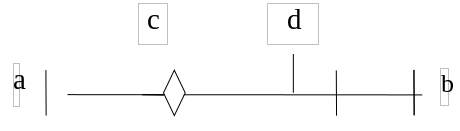
\includegraphics[width=50mm]{./imgs/fig6.jpg}
%\caption{I}
\end{figure}

Ou seja, o momento, entre dois instantes, em que o mundo se torna
visível, o ponto de encontro entre ``isto e aquilo'' (veja"-se o poema
``Nãoagora''). É assim que o poeta se explica em seu diário\footnote{Kharms, 2013, p. 95.}:

\begin{quote}
Se a verdade inteira se expande ao longo da linha \emph{ab}, então o
indivíduo só pode ver uma parte, a que não vai além de \emph{c}, o
limite do possível. (\ldots{}) {[}Valendo"-se da alteração do estado
normal de consciência{]}, certas pessoas podem estender sua percepção a
diferentes partes da verdade universal, por exemplo, até \emph{d}, mas
dificilmente elas terão uma compreensão real do que tiverem ``visto'',
pois terão conhecido apenas duas partes do mundo desconectadas uma da
outra: \emph{ac} e \emph{d.} A verdadeira compreensão lhes adviria do
conhecimento da verdade de \emph{a} até \emph{b}. (\ldots{}) Creio que
existam possibilidades, embora ocultas, de captar a verdade, não
escavando suas partes separadas, mas movendo"-se suavemente além dos
limites do possível \emph{c}, compreendendo a distância em sua
inteireza.


\noindent{}(novembro de 1926)
\end{quote}

Embora tenha sido Drúskin, em 1933, a encontrar a expressão ``certo
equilíbrio com uma pequena falha'' (\emph{parvum peccatum}) --- que no
gráfico seria representado pelo obstáculo \emph{c} --- à qual ---
justamente --- atribuiu um matiz religioso (o protótipo da pequena falha,
no caso, seria Cristo feito homem, Deus tornado real, a imperfeição
somente através da qual é possível compreender a perfeição), o conceito
é arquetípico. (Veja"-se de Calvino \emph{Assunto
encerrado}, em que o autor interpreta o fato de os indígenas sempre
deixarem um fio solto em seus tecidos\footnote{Calvino, Italo. \emph{Assunto encerrado -- discursos sobre literatura
e sociedade}. (Trad. Roberta Barni). São Paulo: Companhia das Letras, 2009.}).

Kharms retoma essa problemática em várias de suas miniaturas. Veja"-se
particularmente o episódio"-obstáculo da fada em ``Sobre o equilíbrio'',
de 1934. Por sinal, Jaccard explica por essa estruturação de ``certo equilíbrio'' o princípio característico da
assimetria que rege a poética de Kharms\footnote{Jaccard, 1995, p. 162.}. Muitas, com efeito, são as
características de sua poética, que, em muitos aspectos fundamentais, é
decorrência de suas meditações filosóficas. Reduzir o objeto à soma de
partículas para poder integrá"-las ao todo, graças à ordem que a Arte
imprime, faz com que sua poética implique a ruptura, como fase
preliminar.

Quando algumas de suas convicções coincidiam com as de personalidades
que ele estimava, Kharms rejubilava"-se. ``Em tudo o que eu faço, eu sou
o criador de uma forma minha no mundo'' --- diz ele, ecoando Bakhtin.
Deslocamento, fluidez, deformação estão entre os fenômenos mais
conspícuos de sua poesia, coincidindo com a visão de Iúri Tyniánov, o
crítico formalista que ele mais apreciava. O intuitivo e o
\emph{transracional} que ele praticava são alguns dos pontos"-chaves de
Khlébnikov, o mestre do futurismo russo por quem tinha especial
predileção. Retirar a palavra do âmbito de sua distribuição normativa e
introduzi"-la num contexto não convencional (a não coincidência de
palavra com coisa), de modo que a palavra se torne livre, assumindo
significados diferentes, tem ligação com a importância que Malévitch
dava à ``situação'' do objeto, mais que à sua essência. O objeto deixa
de ter contornos definidos --- dizia o pintor --- ``e se espalha no
macrocosmo, tal como a palavra que, livre da causa"-efeito
lógico"-gramatical se ergue acima de constrangimentos''.

Como foi dito, Kharms, desde a época do Instituto Eletrotécnico,
desenvolveu estudos de numerologia, que, por ocasião de seu desterro em
Kursk, o levaram a profundas reflexões filosóficas. ``O infinito é a
resposta para todas as questões'' --- diz ele. ``A única pergunta que
merece ser colocada é: o que é o infinito?'' E o zero, que, não tendo
começo, não pode ter fim, permite"-lhe uma série de equiparações
inclusive com Deus: Religião = Harmonia + Deus = zero; Arte = Harmonia =
Ritmo e Beleza = zero; o que lembra o Deus"-zero suprematista de
Malévitch. No grau zero da criação, as palavras, como os sons, voam e
ressoam.

À divindade Kharms sempre apelara nos momentos difíceis à espera de
algum milagre, que não viria. Muitas passagens de seus diários, como foi
visto, se encerram com uma espécie de invocação salvadora --- uma espécie
de fórmula --- que se transformará em constatação no fim de sua
atormentada existência: Deus deu"-lhe os melhores dotes e a vida
obrigou"-o a rastejar nas piores baixezas.

%Os escritos de que consta este livro, de uma comicidade grotesca e
%alógica que desconstrói um mundo tão parecido com o nosso mas que não
%pode deixar de nos surpreender, custaram a internação, a prisão e a
%morte a um jovem autor, hoje considerado um dos máximos representantes
%da literatura do absurdo, entre os mais lidos e os mais publicados no
%Ocidente.

%Bibliografia

%\versal{CALVINO}, Italo. \emph{Assunto encerrado -- discursos sobre literatura
%e sociedade}. Tradução Roberta Barni. São Paulo: Companhia das Letras,
%2009.

%\versal{CHARMS}, Daniil. \emph{Casi}. Organização, tradução e posfácio
%Rosanna Giaquinta. Milão: Adelphi, 1990. (\textsc{giaquinta}: 1990)

%\versal{CHARMS}, Daniil (org. trad. e posfácio Paolo Nori). \emph{Disastri.}
%Turim: Einaudi, 2003. (\textsc{nori}: 2003)

%\versal{JACCARD}, Jean"-Philippe. \emph{Daniil Harms et la fin de
%l'avant-garde russe}. Berna: Peter Lang, 1991.

%\_\_\_\_\_\_\_\_\_\_ \emph{Daniil Kharms i koniéts rússkogo
%avangarda}. São Petersburgo: \emph{Akademítcheskii proekt}, 1995.

%\versal{KHARMS}, Daniil. \emph{I am a Phenomenon out of the Ordinary −
%The Notebooks, Diaries and Letters of Daniil Kharms}. Organização,
%tradução e introdução: Anthony Anemone e Peter Scotto. Boston: Academic
%Studies Press, 2013. (\textsc{kharms}: 2013)

%\_\_\_\_\_\_\_\_\_\_ \emph{Sobránie Sotchiniénii v dvukh
%tomakh}. Moscou: Zebra E, 2010.

%\versal{OSTASHEVSKI}, Eugene (org.). \emph{\versal{OBERIU} -- An Anthology of
%Russian Absurdism}. Illinois: Northwestern University Press, 2006.

%\versal{ROBERTS}, Graham. \emph{The Last Soviet Avant-garde}. Nova York:
%Cambridge University Press, 1997.

%\versal{YANKELEVICH}, Matvei (org.). \emph{Today I Wrote Nothing.} Nova York:
%Overlook Duckworth, 2007.

\part{contemporâneos (século {\MinionPro{\versal{XX}}})}

\chapter{Vladímir Nabókov: arte duradoura e talento individual}

Não por nada a primeira lição de literatura russa de Vladímir Nabókov
(1899--1977) reunida, com nove outras, no livro \emph{Lições de
literatura russa}\footnote{São Paulo: Três Estrelas, 2014.}, tem como fecho o poema
``À maneira de Pindemonte'', de Aleksandr Púchkin (de quem Nabókov
também verteu primorosamente para o inglês o famoso romance em versos
\emph{Evguéni Oniéguin}, transformado em ópera com música de
Tchaikóvski); em poucas linhas, o poema sintetiza o credo de Nabókov ---
seu individualismo sem concessões e a relação conflituosa que se trava
entre o autor e o mundo:

\begin{verse}
Não responder a ninguém, ser seu próprio \\
vassalo e senhor, só agradar a si mesmo. \\
Não curvando a espinha, nem sua vontade \qb{}íntima, \\
nem a consciência (\ldots{}) e sentindo a alma \\
derreter no calor dos desígnios inspirados \qb{}do homem\ldots{}
\end{verse}

Dito isto, que se manifesta em suas opiniões quanto ao regime, aos
censores e aos escritores russos, resta deleitar"-se com suas análises
extraordinárias das obras dos autores russos do século \versal{XIX}, seus
favoritos, não apenas porque representam o pináculo da literatura russa,
mas também --- conforme repara o prefaciador Fredson Bowers --- porque
lhe permitem se contrapor ao utilitarismo dos críticos sociais do século
anterior e dos escritores soviéticos que lhes sucederam.

Em particular, neste livro, ele trata de Gógol (\emph{Almas mortas} e
\emph{O capote}), Tolstói (\emph{Anna Kariênina} e \emph{A morte de Ivan
Ilitch}), Tchékhov (\emph{A dama do cachorrinho}, \emph{No fundo do
barranco} e \emph{A gaivota}) --- autores que admira; de Turguêniev
(\emph{Pais e filhos}) --- que aceita com reservas, justamente pelo apelo
ao elemento social (ao qual Tchékhov, dono de ``toques leves e de
pequenos e inesperados meandros'', sempre resistiu), por suas pausas
tradicionais para o esboço biográfico das personagens e por saciar por
completo a curiosidade do leitor com seus epílogos; de Dostoiévski
(\emph{Crime e castigo}, \emph{Memórias do subsolo}, \emph{O idiota},
\emph{Os demônios} e \emph{Os irmãos Karamázov}) --- que critica: ``Minha
posição em relação a Dostoiévski é curiosa e difícil. Em todos os meus
cursos abordo a literatura a partir do único ponto de vista que me
interessa --- a saber, o da arte duradoura e do talento individual. Dessa
perspectiva Dostoiévski não é um grande escritor, ao contrário, é
bastante medíocre --- com lampejos de excelente humor mas, infelizmente,
separados por oceanos de platitudes literárias''.

Por outras perspectivas que o leitor terá o prazer de percorrer, porém,
reconhece"-lhe méritos, entre os quais o de saber admiravelmente reunir
farsa e tragédia, e de ser um dramaturgo \emph{manqué}. Finalmente
Gorki, que é assim desancado: ``sentindo que precisava encontrar alguma
compensação pela pobreza de sua arte e pelo caos de suas ideias, ele
sempre buscou os assuntos chocantes, o contraste, o conflito, a
violência, a crueldade''.

Quanto a Tolstói, tal como Nabókov pertencente à antiga nobreza
(conhecera"-o com o pai, quando criança), o considera o maior escritor
russo. Para ele, é o exemplo da perfeita estrutura temporal da obra, que
flui como real, juntamente com o tempo do leitor; do domínio som/sentido
(comum também a Gógol, o máximo representante da imaginação literária
eficaz e que não por nada chamou ``poema'' a seu \emph{Almas mortas}),
e da refinada arte dos detalhes que confluem para um mesmo fim (não se
esqueça que Tolstói é um autor que gosta de defender alguma tese em suas
obras), no caso de \emph{Anna Kariênina}, para os males do adultério.

Nas aulas sobre escritores ocidentais que ele ministrou, igualmente, em
várias universidades norte"-americanas, Nabókov ia direto para o estudo das
obras de seus favoritos, explicando"-as com diagramas e com citações
nevrálgicas (era formado em literatura francesa, além de conhecer
perfeitamente o alemão, e, com \emph{Lolita}, foi considerado um dos
mestres de língua inglesa). Entretanto, quando tratava de escritores
russos, dirigindo"-se a um público que desconhecia sua obra e sua
cultura, apresentava um resumo biográfico e uma visão geral do ambiente
e das obras do escritor, antes de passar à análise mais aprofundada das
obras escolhidas, que é o que mais o interessava.

Conforme é sabido, além de escritor e entomologista (tinha por
\emph{hobby}, desde a infância, colecionar borboletas, e em museus
norte"-americanos há espécies por ele descobertas), Nabókov era um inveterado
jogador, estudioso e preparador de problemas de xadrez. ``Em xadrez,
(\ldots{}) há os recursos como o avanço, o recuo, o bloqueio, o desbloqueio e
assim por diante, mas só quando são combinados de uma certa maneira é
que o problema se torna satisfatório'' --- diz Nabókov em sua
autobiografia\footnote{\emph{A pessoa em questão}, Companhia das Letras, 1994,
também traduzida como \emph{Fala, memória}, Alfaguara, 2014.}. Pois bem,
para ele, esses ``recursos'' são, em literatura, o uso e a combinação
dos detalhes: o domínio dos detalhes, ao mesmo tempo científico e
artístico, era a chave com que o leitor inteligente desvendava o segredo
do funcionamento das obras"-primas. ``Nos meus tempos de professor,
esforcei"-me para oferecer aos alunos de literatura a informação exata
sobre os detalhes, sobre as combinações de detalhes que produzem a
centelha sensual sem a qual o livro é algo morto''\footnote{\emph{Cf}. \emph{Introdução}
de Fredson Bowers às \emph{Lições de literatura russa}.}.

Vejamos, para terminar, alguns exemplos de como os detalhes em
\emph{Anna Kariênina} de Tolstói funcionam como chave para a
interpretação da obra. No trem de volta a São Petersburgo, depois do
encontro fatal com Vrónski, Anna está lendo um livro, e a criada, que a
acompanha, tem ``as mãos largas enfiadas em luvas de lã, uma das quais
rasgadas na ponta de um dos dedos'' (``Reparem'' --- diz o
professor, entre parênteses, --- ``o pequeno defeito
correspondendo ao transtorno no estado de espírito de Anna'').
Sempre no vagão do trem: ``Notem que o quente e o frio estão se
alternando também no vagão"-dormitório'' e assim, num crescendo, até
analisar o sonho duplo (de Anna e de Vrónski) em que aparece o mesmo
anão maltrapilho, que Tolstói, antifreudianamente, analisa como sendo o
símbolo do pecado de ambos. ``De seu pecado imundo e deformador da alma
--- as duas imagens se mesclando num clarão funesto''.

\chapter{Prefácio a Bródski}

--- Escrevo poesia desde os dezoito anos --- declarava Ióssif Bródski
(1940--1996) a seu entrevistador Michael Skammel, da Revista \emph{Index
on Censorship}, n. 3/4 (versão russa), de outubro de 1972. Alguns meses
antes, em junho, Bródski era expulso da \versal{URSS} e chegava a Viena, onde
encontrava, em sua casa de veraneio, W. H. Auden, o poeta
anglo"-americano que ele mais admirava e que havia concordado em escrever
uma introdução a um volume de seus poemas, organizados e traduzidos por
G. L. Kline, que contatara em Leningrado, ainda em 1969, para uma
futura edição da \emph{Penguin}. Auden solidarizou"-se com ele e o apresentou ao
meio intelectual vienense. Após participar com ele, em Londres, de um
encontro internacional de poetas, onde conheceu Isaiah Berlin, Seamus
Heaney e Robert Lowell, Bródski recebeu um convite para lecionar na
Universidade de Michigan, para onde se dirigiu, no mesmo ano de 1972. Em
1977, se naturalizou americano. ``Sou judeu, poeta russo e cidadão
estadunidense'', assim ele se apresentava, apesar das muitas obras, em
prosa e em verso, que teve ocasião de escrever diretamente em inglês.

--- Mas por que foi processado? --- indagava o entrevistador.

--- Realmente não sei. De qualquer modo, é típico do Ocidente, quando
aborda esse problema, achar que qualquer acontecimento e qualquer
fenômeno deva ter sua explicação. Tudo isso é muito complicado. Claro,
tudo tem sua razão de ser. No que se refere ao porquê me condenaram, a
única coisa que posso fazer é remeter aos atos da acusação. A minha
opinião pessoal, que certamente não irá satisfazê"-lo, é muito simples. O
indivíduo que começa a construir seu mundo pessoal, independente, mais
cedo ou mais tarde acaba se tornando um corpo estranho para a sociedade,
acaba se tornando objeto de todo tipo de distanciamento, achatamento,
opressão.

--- E como explica que o tenham solto tão rapidamente?

--- Honestamente, não sei.

Bródski havia sido condenado a cinco anos de trabalhos forçados, em
seguida reduzidos a cerca de um ano. A esse respeito, precisa Carole
Seymour"-Jones, em seu livro \emph{Uma relação perigosa}: ``Ehrenburg
insistia com Sartre para que escrevesse para Mikoyan e pedisse perdão
para Bródski que fora mandado para uma fazenda estatal nos arredores de
Arkhanguelsk. Ele o fez, numa carta notavelmente servil. Pouco depois,
Bródski foi perdoado''.

--- Qual é a utilidade de seus ``assim chamados versos''?

Esta pergunta sintomaticamente acintosa é repetidamente formulada pela
juíza encarregada do processo de Leningrado de fevereiro de 1964 ---
que costuma ser reproduzido na parte que foi permitida à jornalista Frida A.
Vigdórova estenografar --- em que Bródski, então com 24 anos de idade,
era acusado de ``parasitismo social''. As respostas com que o poeta
tentou, sem sucesso, se defender na ocasião e que haveriam de tornar"-se
pressupostos teóricos de sua obra, foram reelaboradas mais de vinte anos
mais tarde, vindo a constituir uma síntese de interessantes reflexões
sobre a arte, entre outros, na coletânea de ensaios \emph{Menos que um}
(a Companhia das Letras, em 1994, publicou, com este título, cerca de
dois terços do original em inglês \emph{Less than one}) e no
discurso proferido por ocasião da outorga do Prêmio Nobel, em 1987.

Neste último, cujos pontos principais sintetizamos, Bródski como que
desenvolve a defesa que não lhe foi permitido apresentar no processo,
quando era repetidamente acusado de não pertencer a nenhum círculo e de
não trabalhar para o progresso da coletividade.

``O que a arte ensina, se é que a arte ensina alguma coisa --- ao
artista, em primeiro lugar'' --- diz ele ---, ``é a privacidade da
condição humana''. Sendo o mais antigo e o mais literal dos
empreendimentos humanos, o fazer artístico, tanto em termos de criação
como em termos de fruição, infunde ao criador/fruidor um sentido de
unicidade, de individualidade que o destaca do \emph{socium}, tornando"-o
autônomo. A leitura de um poema, por exemplo, dirige"-se ao leitor num
\emph{tête"-à"-tête}, entrando com ele numa relação direta, sem
intermediários. Por isso a poesia não costuma ser regida pelos padrões
de ``bem comum'' ou ``necessidade histórica'' ou, tanto menos, de
``consenso'' ou ``unanimidade''.

A essa unicidade somos preparados geneticamente, e a tarefa de cada um
consiste em dar conta da própria vida (o \emph{presente} contínuo), de
uma maneira não imposta nem prescrita por ninguém (o \emph{passado},
sobrestando a esse presente). Da mesma forma, a língua e
consequentemente a literatura --- que são as mais antigas, as mais
inevitáveis e as mais duráveis entre todas as organizações humanas ---
quando manifestam ironia, indiferença, ou dissenso em relação ao Estado
[aí está o \emph{punctum dolens}], representam o permanente (melhor ainda, o infinito) contra o temporário, o finito. A ética do
Estado, sem mencionar a sua estética, são sempre o passado, gravando
sobre o presente da língua, ou mesmo sobre o futuro que a obra de arte
representa, quando leva quem lida com ela para além do esperado, do
suposto. Um dos méritos da literatura é tornar o tempo da existência
mais específico, fazer com que o indivíduo se diferencie da multidão
{[}globalizada --- acrescentaríamos hoje{]} --- fazer com que ele evite a
tautologia. O que torna a arte em geral e a literatura em particular
notáveis é que ambas abominam a repetição. Na vida de todo dia você pode
contar uma piada três vezes e, provocando o riso três vezes, tornar"-se o
animador da festa. Na arte, este tipo de conduta tem o nome de
\emph{clichê.}

Uma vez que o significado privilegiado da existência humana é, no
entender do poeta, a aquisição de um rosto não comum, e sendo a
estimulação da diversidade humana justamente a razão de ser da
literatura, decorre que a estética é a mãe da ética, ou seja, em sentido
antropológico: antes de ser uma criatura ética, o ser humano é uma
criatura estética. Vejam"-se as criancinhas --- diz Bródski. Se elas
choram diante de certas pessoas e sorriem a outras {[}a tão decantada
``primeira impressão''{]}, não é a ética que as leva a isso, é a
estética. E ainda, mais especificamente, se aquilo que nos diferencia
dos outros animais é a palavra e, em sendo o poeta o instrumento de que se
serve a língua para existir e renovar"-se, a poesia --- enquanto
realização suprema da palavra --- é o objetivo privilegiado de nossa
espécie. Se a poeticidade é o que faz sobreviver uma obra de arte, a
poeticidade é a ética da linguagem.

Uma arte como a música, por outro lado, pode admitir um ouvinte passivo
ou outro, ativo, que a interprete, enquanto que a poesia, sendo
``desesperadoramente semântica'' {[}Cf. o poeta Eugenio Montale, citado
pelo autor{]}, admite tão somente este último. Com isso dá"-se uma
equiparação entre a consciência do autor e a do fruidor, fato que, mais
cedo ou mais tarde --- no dizer de Bródski --- acaba condicionando a
conduta do indivíduo. Quanto mais rica for a experiência estética, tanto
mais segura será a escolha moral e tanto mais livre o homem. Daí o
famoso dito de Dostoiévski de que a beleza salvará o mundo. A arte anima
a realidade e corre paralela à história, não é seu sinônimo. ``E a
maneira pela qual a arte existe é criando continuamente uma nova
realidade estética. Eis porque ela se encontra, tantas vezes, `à frente
do progresso', à frente da História, cujo principal instrumento é ---
longe de nós o propósito de, mais uma vez, querer aprimorar a Marx ---
justamente, o \emph{clichê}''.

Os poetas dizem a História através de sua linguagem progressiva. A
literatura é o antídoto que temos contra a lei da jangal: uma existência
que ignora os critérios propostos pela literatura é uma vida inferior.
Recorremos à poesia por razões inconscientemente miméticas. Por utilizar
o modo analítico de cognição, mas orientar"-se principalmente para os
modos da intuição e da revelação, o exercício poético é um acelerador da
consciência. Enfim, literalmente: ``A sociedade, maioria por definição,
presume ter outras opções que não sejam as de ler versos, por mais bem
escritos. Ao deixar de ler versos, entretanto, arrisca"-se a cair naquele
nível de elóquio em que uma sociedade é presa fácil de demagogos e
tiranos''.

Além dessas suas ``respostas'', em vários modos reiteradas, às
acusações de que foi objeto, Bródski não tinha em mente nenhuma
ideologia em particular, nem se pautava por nenhuma filosofia de vida:
``Eu tenho uma série de convicções'' --- teria ele respondido à
pergunta de um jornalista, conforme relata Lev Loseff (escritor russo emigrado
para os \versal{EUA} em 1976, autor de uma biografia do poeta escrita
originariamente em russo e traduzida para o inglês como\emph{Joseph
Brodsky: a literary life)} --- ``se quiser
chamar a isso de filosofia, eu a chamaria de filosofia da
\emph{endurance} ---da possibilidade, da capacidade de resistir''.
``Não sou um ser moral (mesmo se procuro estar quite com minha
consciência) ou um sábio'' --- escreveu ele em \emph{Margem dos
incuráveis} (\emph{Watermark}) --- ``não sou sequer um filósofo ou um
esteta. Sou apenas um homem nervoso, consequência das circunstâncias e
dos meus atos, mas sou observador''. A vista é soberana na percepção de
Bródski: ``O olho precede a pena, e não permito à minha pena de mentir
quanto à sua posição''.

Por outro lado, quem ler \emph{Menos que um}, a coletânea dos ensaios
mais importantes de Bródski publicada nos \versal{EUA} em 1986, --- e aqui
retomo trechos de resenhas que escrevi para jornais de São Paulo ---,
confrontar"-se"-á com uma série de considerações instigantes sobre a visão
do mundo de hoje e a criação poética, que se tornam tanto mais
reveladoras quando comparadas depois com sua própria obra (aqui, entre
nós, uma amostra muito feliz de sua poesia são os sete poemas publicados
em 1995 pela 7Letras com o título de \emph{Quase uma elegia}, na
tradução de Boris Schnaiderman e Nelson Asher).

Mesmo sendo verdade --- como diz Bródski --- que a biografia de um poeta
está em sua ginástica com a linguagem, não deixa de ser sintomático o
desejo irrealizado, e por ele várias vezes expresso, de poder olhar para
trás e conseguir discernir os pontos de inflexão de sua vida, de sua
evolução: ``Se existe algo que eu possa chamar de marco, é aquilo que
não serei capaz de reconhecer eu mesmo --- ou seja, a morte''. Quando ela
ocorreu (o poeta ia completar 56 anos quando morreu de infarto), o que
ele escreveu adquiriu subitamente outra dimensão. Ora certas conclusões
se transformam em ditos: ``O talento não precisa ser história'', ``O
sofrimento não é matriz de uma arte superior'', ``O amor ocupa mais
lugar na mente que no leito''; ora certas divagações se condensam em
aforismos, como, por exemplo, o que deu origem ao título do referido
livro de ensaios. No âmbito da escritura --- diz o poeta --- onde
contrariamente a outros domínios tudo o que se acumula é incerteza, a
infância, a adolescência, a idade adulta não são categorias distintas,
elas se confundem. A insatisfação de um menino com o controle dos pais e
o pânico de um homem diante de uma responsabilidade são da mesma
natureza: ``Não se é nem um nem outro desses personagens; é"-se, talvez,
menos que um''. Por isso mesmo ele não acredita que todas as chaves do
caráter devam ser buscadas na infância: se assim fosse, o que seria ---
pergunta"-se ele --- das três gerações de russos que, como ele, viveram
apinhados em apartamentos comunais, fingindo não verem os pais na cama,
à noite, e ouvindo mentiras oficiais na escola e oficiosas em casa?

A ``quasidade'' da verdade levou, entretanto, muitos a se adaptarem
àquilo que ele considerava o traço mais marcante do leste europeu como
um todo --- a ambivalência, que ele condenava e cujos efeitos resumia no
dístico tomado emprestado de ``O escudo de Aquiles'' de Wystan Hugh
Auden, que ele considerava o poeta mais inteligente do século \versal{XX}:
``\emph{they lost their pride}/\emph{and died as men before their
bodies died}''.

Para ele, obviamente, o efeito foi o oposto. Conforme é sabido, o jovem
Bródski escolheu o caminho da recusa: com quinze anos abandonou a escola
e após várias peripécias, entre as quais constam sua prática como
operário numa obsoleta fábrica de canhões e sua estada como aprendiz no
obitório do hospital que ficava ao lado da maior prisão da Rússia, em
Leningrado, acabou sendo exilado para os \versal{EUA} em 72, após o processo
farsesco que se irá ler. ``Uma das vantagens do totalitarismo'' ---
escreve o poeta --- ``é que ele sugere ao indivíduo certo grau de
hierarquia pessoal que tem, no vértice, a consciência. Assim vigiamos o
que acontece dentro de nós mesmos: pode"-se dizer que denunciamos à nossa
consciência o comportamento de nossos instintos. E castigamos com nossa
consciência o comportamento de nossos instintos. E nos castigamos com
nossas próprias mãos. (\ldots{}) Não que eu ache que o mecanismo da repressão
é inato na psique humana tanto quanto o mecanismo da liberação''. É esta
consciência pessoal cada vez mais crítica e cada vez mais abstraída da
norma coletiva que o leva a formular opiniões às vezes surpreendentes,
mesmo em termos de teoria literária.

``No seu livro de ensaios \emph{Less than one}'' --- foi"-lhe perguntado
por Nelson Asher, por exemplo, numa entrevista para a \emph{Folha de S. Paulo},
em agosto de 1987 --- ``você tem textos sobre os poetas russos Anna
Akhmátova, Marina Tsvetáieva, Ossip Mandelstam, mas você não escreve
sobre Vladímir Maiakóvski, Boris Pasternak ou Velimir Khlébnikov, que
são geralmente considerados poetas tão importantes como os outros três.
Por quê?

Bródski: ``Eu os considero figuras menores, sobretudo Maiakóvski. Minha
atitude pode ser idiossincrática. Mas eu não pretendo que meu gosto ou
meu julgamento sejam aceitos por todos. Khlébnikov é mais um fenômeno
literário do que um verdadeiro poeta. Pasternak, por sua vez, é um ótimo
poeta, mas devido à bagagem metafísica, à sua mensagem metafísica, ele é
bem menos interessante que, por exemplo, Tzvetáieva. Quanto a
Maiakóvski, ele é um fenômeno interessante e um bom poeta, especialmente
nos poemas da juventude, mas eu simplesmente não gosto dele''.

Ou então, ainda na coletânea citada, no ensaio sobre Mandelstam, ele
afirma: ``O simbolismo foi sem dúvida o último grande movimento (e não
apenas na Rússia), só que a poesia é uma arte extremamente
individualista e não aceita `ismos'. (\ldots{}) Com o final do século
chegou"-se à crise do simbolismo, já então comprometido por uma espécie
de inflação verbal semelhante àquela que na América de hoje aconteceu ao
verso livre''.

Se na vertente russa Bródski sentia"-se atraído pelos versos de
Akhmátova, Tsvetáieva e Mandelstam, na vertente anglo"-americana --- a sua
preferida, desde os tempos de rapaz, (quando, na sua turma, --- conforme
ele recorda --- ``uma amizade podia terminar para sempre pela preferência
dada a Hemingway antes que a Faulkner'') --- seus ídolos eram Samuel
Beckett, Robert Frost mas, principalmente, W. H. Auden. A este último
ligou"-se por amizade pessoal, quando foi procurá"-lo tão logo se exilou,
na casa onde ele morava na Áustria, dois anos antes de Auden morrer. A
elegia que Bródski escreveu em inglês, em memória do amigo, ``Para
contentar uma sombra'' [que consta do livro \emph{\versal{W. H.} \versal{AUDEN}}
(\emph{Poemas})], tornou"-se o marco de sua nova identidade
literária. O poeta Ióssif Bródski da primeira grande coletânea de poemas
reunidos sob o título de \emph{Parte do discurso} (1980) passou a ser,
também, Joseph Brodsky, poeta bilíngue, tendo traduzido ele mesmo um
número considerável de seus antigos poemas para o inglês ou composto
novos diretamente nesta língua, no volume de versos \emph{Para Urânia},
publicado em 1988.

Na oração fúnebre para o amigo (não por nada as elegias são
``involuntárias tentativas de autorretrato''), Bródski realça uma série
de aspectos que são também traços de sua própria poesia. O tom pacato,
sem pedal e sem ênfase, os matizes neutros, o anti"-heroico, a paródia
fulminante, o aparentemente coloquial e o metafísico disfarçado de senso
comum. Isso tudo, porém, regido por metros peculiares, que por serem o
equivalente do ritmo, são uma grandeza ``anímica'', configuram uma
harmonia própria de cada um como a respiração ou o batimento cardíaco.

A crítica fala em naturezas mortas, em presenças e ausências, mais que
em temas de sua poesia, em trocadilhos, rebus, adivinhas, mas
principalmente em ambiências. Não se esqueça que para Bródski era na
geografia e não na história que devia ser procurado o início de todo
conhecimento. Nesse sentido, vale a pena exemplificar com algumas
matrizes imagéticas características de sua poesia, que aparecem no poema
considerado sua ``certidão de nascimento'':

\begin{verse}
Nasci e cresci nos pântanos do Báltico, \qb{}lugares \\
onde ondas cinza de zinco sempre correm \qb{}aos pares, \\
daí todas as rimas e a voz atenuada que \\
entre elas se enrola, qual cabelo molhado; \\
se é que se enrola. Mesmo o cotovelo \qb{}fincado, \\
a concha do ouvido não distingue nelas \qb{}nenhum chiado, \\
apenas bater de telas, de postigos, \qb{}de palmas, o apito \\
da chaleira, fervendo no fogão --- no máximo \qb{}--- o grito \\
das gaivotas. Nessas plagas planas o que \qb{}retém \\
do falso o coração é que não há onde \qb{}esconder"-se e vê"-se além. \\
Apenas para o som o espaço é sempre \qb{}obstáculo: \\
pela falta de eco não se queixa o olho.
\end{verse}

E nesse outro, com o título de ``24 de maio de 1980'', lembrado por
Piotr Kilanowski, professor da \versal{UFPR}, que, traduzido a partir da versão russa mas abrindo o volume
\emph{To Urania}, em transcrição inglesa pelo próprio
autor, pode ser considerado a antecipação de seu epitáfio:

\begin{verse}
Entrei na toca com feras selvagens, \\
Preguei meu nome e data na barraca, \\
Joguei roleta, morei no mar, à margem, \\
Jantei de fraque com sabe o diabo quem. \\[8pt]
Do alto da geleira avistei meio mundo, \\
Tres vezes me afoguei, duas vezes me \qb{}cortaram. \\
Larguei a pátria que me alimentara, \\
Uma cidade nasce dos que me esqueceram. \\[8pt]
Vadiei pelas estepes ao urrar dos hunos, \\
Vesti o traje que de novo está na moda, \\
Plantei centeio, forrei o celeiro com betume, \\
A não ser água seca, bebi tudo. \\[8pt]
Sonhei com a pupila turva do guarda do \qb{}comboio, \\
Devorei o pão do exílio sem deixar migalha. \\
Abri minhas cordas aos sons, fora o do aboio; \\
Tirei"-lhes a vibração. Sou agora quarentão. \\[8pt]
O que dizer da vida? Que resultou comprida. \\
Só na desgraça sinto a comunhão. \\
Mas enquanto não encherem de barro a \qb{}minha boca \\
dela ressoará somente a minha gratidão.
\end{verse}

(A tradução desses dois poemas finais é de minha autoria).

%Bibliografia:

%\versal{AUDEN W. H.}. \emph{\versal{W. H. AUDEN.} [Poemas]} (trad. José Paulo Paes e
%João Moura Jr.). São Paulo: Companhia das Letras, 2013, p.245.

%\versal{BRÓDSKI}, Ióssif. \emph{Kniga Interviu} (\emph{Livro das Entrevistas}).
%Moscou: Zakharov, 2007, p.7-12

%\versal{BRÓDSKI}, Ióssif. \emph{Náberejnia nieistslelímikh} (\emph{Margem dos
%incuráveis - Watermark}) (Edição bilíngue, russo-ingles). São
%Petersburgo: Azbuka-Klassika, 2007, p.19

%\versal{BRODSKY}, Joseph. \emph{To Urania.} New York: The Noonday Press, 1992

%\versal{BRODSKY}, Joseph. \emph{Menos que um.} São Paulo: Companhia das Letras,
%1994

%\versal{BRODSKY}, Joseph. \emph{Quase uma elegia} (Ed. bilíngue russo-portugues
%. Trad. Boris Schnaiderman e Nelson Asher). RJ: Sette Letras, 1995,
%p.51-52

%\versal{BRODSKIJ}, Iosif. \emph{Poesia} (Ed. bilíngue russo-italiano. Org.
%Giovanni Buttafava) Milano: Adelphi, 1988

%\versal{BRODSKIJ}, Iosif. \emph{Fuga da Bisanzio} (\emph{Less than One}) (Trad.
%Gilberto Forti). Milano: Adelphi, 1987

%\versal{BRODSKIJ}, Iosif. \emph{Dall' esilio} (\emph{The condition we call exile;
%Nobelévskaia retch, Acceptance Speech}). Milano: Adelphi, 1987

%\versal{LOSSEF}, Lev. \emph{Joseph Brodsky -- a literary life.} (Trad. Jane Ann
%Miller). New Haven \&London: Yale University Press, 2011, p.139

%\versal{SEIMOUR-JONES}, Carole. \emph{Uma relação perigosa} (\emph{Uma biografia
%de Simone de Beauvoir e Jean-Paule Sartre}. R.J.: Record, 2014, p.469)

\chapter*{Um escritor russo na América -- Dovlátov: \emph{Parque Cultural} e \emph{O ofício}}

\addcontentsline{toc}{chapter}{Um escritor russo na América -- Dovlátov}
\hedramarkboth{Um escritor russo na América -- Dovlátov}{}

Serguei Dovlátov (1941--1990) é um nome importante não apenas na
literatura russa de hoje, mas também na dos \versal{EUA}, para onde emigrou (1978) e se tornou famoso como fundador do jornal \emph{O novo
americano}, foi reconhecido pelas mais prestigiosas revistas (\emph{New
Yorker} e \emph{Partizan Review}), lançou 12 livros, e lhe foi dedicada
uma rua (\emph{Sergei Dovlatov way} --- no Queens).

Já o parque ``Serguei Dovlátov'' que lhe foi dedicado na Rússia de
hoje, quando se tornou um autor icônico, entre os mais queridos, tem a
ver com esta curiosa novela, uma das mais comicamente ferinas que se
possam ler na literatura russa atual. Acontece que na Rússia de Púchkin
(1799--1837) havia uma propriedade, na região de Mikháilovskoie (perto de
Pskov --- norte do país), onde o grande poeta costumava passar suas
férias (e exílio), que na época da \versal{URSS} foi transformada em
\emph{Parque Cultural} e monumento histórico. Um parque, onde foi
recriado o ambiente da época do poeta nacional, retocado (leia"-se
``fajutado''), aberto à visitação pública, e onde Dovlátov trabalhou
como guia turístico pouco antes de emigrar, parque esse que para Borís
Alikhánov (seu \emph{alter ego}, na novela) é uma alegoria da própria
vida na \versal{URSS}. Mas descrita com tanto humor (cáustico) pelo protagonista
e narrador Alikhánov, que se autoironiza (como o Humbert Humbert de
\emph{Lolita} ou o nosso Serafim Ponte Grande) dizendo, com a sua
inconveniência politicamente incorreta, disparates que muitos ``pensam,
mas não dizem'', entremeados por generalizações comuns ao mundo inteiro
(liberdade, amor, morte, impostura, vícios: em especial --- sexo e
bebida), expressas com uma hilariante ingenuidade \emph{non"-sense} que
conquista a simpatia do leitor a cada página.

Na verdade, como muitos artistas, o autor recria nas obras, publicadas
após sua emigração (todas, tirante alguns contos em \emph{samizdat} que
foram bem recebidos e que, apesar de desconstruírem o mito soviético,
nunca provocaram rejeição), fatos e figuras das etapas de sua vida
real. Seu malogro inicial na literatura oficial foi, inicialmente, ele
ter passado a constar, em 1968, de uma ``lista negra'' (dos
participantes do ``Sarau da juventude criativa de Leningrado'') --- coisa
que ele só descobriu mais tarde: ``Na União Soviética eu não era
dissidente. (A bebedeira não conta). Eu apenas escrevia contos alheios à
ideologia\ldots{} Publicam qualquer um, menos eu. As pessoas vendem a alma ao
diabo, eu a dei de graça\ldots{}''

Sua infância/juventude/maturidade aparecem nos contos de \emph{Os
nossos} (1977): a família, os amigos; \emph{A mala} (1986): o resumo
de toda sua vida na \versal{URSS}; \emph{O ofício} (1985): este, sobre sua
``carreira'' na \versal{URSS} e na América, já publicado em português; \emph{A troca} (1981): período
de 5 anos em que trabalhou em Tallin como jornalista, encerrado por
outro malogro completamente casual; \emph{A zona} (1982): seu serviço
militar como membro da ``tropa da prisão''; e nas novelas curtas
\emph{A estrangeira} (1986): sobre a emigrada Mússia Tataróvith; \emph{A filial} (1990), etc.

O eixo de \emph{Parque Cultural} (1983) é a separação da mulher do
narrador (Tânia, na novela) que emigra com a filha para os \versal{EUA} (o pai do
ex"-marido é judeu) bem no momento em que, apesar da bebedeira e de uma
série de quiproquós com figuras impagáveis (os turistas, que às vezes
desmaiavam de tensão, a metodologista, de corpo indistintamente feio, o
senhorio bêbado, o guia preguiçoso\ldots{}), Alikhánov achava ter conseguido
uma certa harmonia. ``Decidi ponderar tudo com calma. Tentar dissipar a
sensação de catástrofe, de beco sem saída. A vida se desenrolava como
imenso campo minado. E eu estava bem no meio dele. Era necessário
dividir este campo em setores e pôr mãos à obra\ldots{}''. Mas os fatos não o
permitem, ele cai em depressão, volta ao vício e vê"-se acossado pela
censura que sempre, nos momentos culminantes de sua tão desejada
carreira literária, reúne indícios para não publicá"-lo. Estamos na
véspera das Olimpíadas de 1980, época em que se procurava fazer com que
os ``indesejáveis'' saíssem do país e --- de fato ---, na vida real,
apesar de não querê"-lo (``é possível sobreviver e continuar escrevendo
longe de seu leitor e de sua língua?''), Dovlátov, com a mãe e a
cachorrinha de estimação, acaba deixando o país, rumo aos \versal{EUA}, onde, como
previra seu amigo Joseph Bródski que o admirava, terá sucesso de crítica
e de público.

Quando o escritor morreu, em 1990 (de uma parada cardíaca, consequência
da bebida que nunca abandonou), a Rússia lançou oficialmente sua
primeira coletânea de contos. O sucesso foi estrondoso. Sua obra
completa foi publicada em três volumes (1995), saíram pesquisas,
biografias, memórias, filmes, congressos, documentários sobre ele e sua
obra. A casa alugada pelo escritor perto do \emph{Parque Cultural}, que
se encontra na aldeia que no livro aparece com o nome de \emph{Sosnovo,}
tornou"-se sede de um museu no parque que hoje leva seu nome.

Quanto a \emph{O ofício} (Kalinka/Hedra, 2018), trata-se de um livro (publicado primeiramente em New York, em 1985), do escritor emigrado, já conhecido no Brasil pelo hilariante Parque Cultural(Kalinka, 2017).

``Ler Dovlátov é algo leve. Ele como que não reivindica atenção, não insiste em suas conclusões ou observações sobre a natureza humana, não as impõe ao leitor. Eu devoro seus livros em três ou quatro horas de leitura ininterrupta: justamente porque é difícil escapar de seu tom despojado. Ao ler seus contos e novelas, invariavelmente nos sentimos gratos pela ausência de pretensão, pelo olhar ponderado sobre as coisas\ldots{}''

Assim escrevia o poeta Joseph Bródski  ``Ao Seriôja Dovlátov'', dois anos após a morte repentina deste numa ambulância em 1990, num elogio ao amigo, também emigrado nos \versal{EUA}, onde Dovlátov, a partir de 1979, publicara nada menos que doze livros. E é isso é o que sentimos nós, leitores, ao lermos esse seu \emph{O ofício} que, na sua primeira parte, descreve ``alguns dias na vida do jovem Serguei Dovlátov''. Seu entourage, a boemia leningradense e suas vicissitudes, os cafés e as redações que não queriam saber de publicar seus escritos, seus galanteios, suas bebedeiras. 

Há caracterizações engraçadíssimas no ``livro invisível'' (é assim que ele chama a primeira parte), cujos comentários ele reserva para si próprio, nas considerações que ele denomina ``Solos na Underwood'': 

\begin{quote}
Pelo bulevar, ao longo de banquinhos amarelos, diante das lixeiras de gesso, caminha um homem de baixa estatura. Seu nome é Anatóli Náiman.
Suas pernas lestas são revestidas por jeans claros americanos. Em seus movimentos se nota a graça de um jovem príncipe. Náiman é um cowboy intelectual. Ele aperta o gatilho antes de qualquer oponente. Seus chistes afiados estão repletos de veneno. 

\begin{center}
\versal{SOLO NA UNDERWOOD}\\
\end{center}
Uma mulher no bonde diz a Náiman: \\
``Ah, não me toque!'' \\
``Não faz mal, depois vou lavar as mãos\ldots{}''
\end{quote}

Ou então, outro \versal{SOLO}:

\begin{quote}
``Tólia'', digo a Náiman, ``vamos visitar Liova Rýskin''. \\
``Não vou. Ele é um  tanto soviético''. \\
``Como soviético? Você está equivocado!'' \\
``Então é antissoviético. Qual a diferença?\ldots{}''
\end{quote}

Paradoxos dessa natureza tornam não menos divertida (e mesmo assim, percuciente) a descrição, na segunda parte do livro, de suas experiências na América, muito próximas da autobiografia. Querendo publicar um novo jornal russo (``O Espelho''), ele e um grupo de companheiros emigrados resolvem procurar um financiador.

``Na casa da tal Cíntia'' --- prosseguiu Móker --- ``volta e meia aparece um italiano. Eu topo toda hora com ele no elevador. Por sinal, ele só vai visitá-la de dia. Daí Cíntia imediatamente corre as cortinas. Que conclusão podemos tirar?''

(\ldots{})

--- ``Daí podemos concluir que Rizzo é dono de um estabelecimento noturno. Por isso faz amor apenas de dia. E todos os estabelecimento noturnos são controlados pela máfia''.

Os amigos marcam encontro com o ``mafioso'' na esquina da Dezessete com a Quinta Avenida e, depois de vários coquetéis expõem ao italiano seu projeto.

\begin{quote}
``Não tocaremos em seu programa ideológico'' --- diz"-lhe Móker. ``Nós apreciamos lutadores honestos, pouco importam suas convicções. Ouvi falar muito de sua organização. Pessoalmente, os objetivos e, especialmente os métodos dela não me são familiares. Mas estou habituado a honrar a firmeza e a valentia em qualquer forma de manifestação\ldots{} Estou ciente que as leis da organização são severas''.

Rizzo assentiu com a cabeça, orgulhoso: --- ``Sim, a organização liquida instantaneamente quem a trai. Não é de se invejar o destino de quem descumpre a palavra dada à organização\ldots{}''
\end{quote}

Qual não é o espanto da turma quando, ao falarem em dinheiro, assim responde Rizzo:

-- ``Claro, eu falarei com o Rafael. Ele administra o caixa do partido. Francamente, duvido que aceite. Rafael é um pouco conservador. Estou certo que ele é muito mais conservador do que seu ídolo, Trótski. Nossa facção de maoístas de esquerda se encontra bem distante do centro\ldots{}''

Sempre à procura do capital inicial para o jornal, Lémkus, outro companheiro que também escrevia para o velho (e único) jornal russo local \emph{Palavra e ação} artigos como ``Como encontrar Deus'', explica:

\begin{quote}
--- ``Vocês simplesmente não conhecem a vida na América. Aqui existem métodos de enriquecimento comprovados e dentro da lei. O que poderia ser mais simples? Você anda pela luxuosa avenida Madison. Em sua direção vem um cachorro, um puro dobermann. Você diz: `Ah, que cachorro bonitinho!'. E, com um movimento rápido, dá-lhe um piparote no nariz. O dobermann engancha sua perna. Você desmaia. Constatam um choque nervoso. Você telefona para um bom advogado. Processa o dono do dobermann. Pede uma indenização por danos físicos e morais. O dono-milionário assina um cheque de pelo menos vinte mil\ldots{}''

--- ``E se for verificado que o cachorro pertence a um mendigo? Será que na Broadway há poucos aleijados negros com dobermanns?''

--- ``Não estou falando da Broadway. Estou falando da Madison. Lá só dá milionário\ldots{}''
\end{quote}

Apesar do sucesso de público e de crítica do novo periódico, finalmente financiado por Larry (``O objetivo da gazeta será aproximar os leitores do Deus judeu e da tradição sionista'') e de seu fracasso financeiro (a redação acaba incendiada), o narrador em primeira pessoa consegue, graças à ajuda da atraente tradutora, Lynn Farber, ter contos seus  publicados pela \emph{New Yorker}. E mais, há um agente literário, Charlie, que lhe encomenda vários romances.

\begin{quote}
Eu só pensava: acontece cada coisa! Um americano, falante de outra língua, ainda por cima ``meio vermelho'', de esquerda, tornou"-se mais próximo e mais compreensível do que meus velhos amigos. As relações humanas possuem um quê de mistério\ldots{}
\end{quote}

\chapter*{Friedrich Gorenstein: \emph{Salmo}, um romance"-meditação sobre os quatros flagelos do Senhor}

\addcontentsline{toc}{chapter}{Friedrich Gorenstein: \emph{Salmo}}
\hedramarkboth{Friedrich Gorenstein: \emph{Salmo}}{}

Intrigante e apaixonante é \emph{Salmo} (1975) de Friedrich Gorenstein (1932--2002), autor judeu russo praticamente desconhecido no Brasil (apesar de ter sido roteirista, entre outros, de \emph{Soláris}
e \emph{Andrei Rubliov} de Tarkóvski). O livro é, como quer o autor,
``\emph{um romance"-meditação sobre os quatro flagelos do Senhor}'' e,
por sua temática, construção e estilo é, entre suas obras"-primas
(\emph{Tchok"-tchok -- romance erótico"-filosófico, Expiação, A casa com a
torre, O lugar)}, a que pode ser considerada a mais importante.

O romance narra nada menos que a vinda do Anticristo em 1933, numa
pequena aldeia da Ucrânia e suas peripécias pela Rússia stalinista até
1973, ano em que desparece. As etapas de suas andanças são pontuadas por
projeções entre profecias da Bíblia e acontecimentos realistas da Rússia
do século \versal{XX} (deskulakização, grande fome na Ucrânia, invasão alemã,
repressões stalinistas, o \emph{homo sovieticus}, o lugar do judeu na
sociedade soviética), época e lugar em que se desencadeiam os flagelos
impostos por Deus aos homens, como punição por seus terríveis desmandos.

Cada um dos capítulos descreve um flagelo (a espada, a fome, a doença e,
particularmente, a luxúria --- ``o animal selvagem que ao dilacerar,
frutifica'') e seus envolvidos que o Anticristo não perde de vista. A
estrutura de cada capítulo é curiosa: um preâmbulo teológico"-filosófico
em que ora se defrontam o Antigo e o Novo Testamento, ora Moisés, que
veio para amaldiçoar os pecadores e defender as vítimas, e Cristo (o
irmão do Anticristo), que veio para perdoar aos pecadores e acenar a
eles e às vítimas com a vida eterna, traído não apenas por Judas mas
pelos apóstolos que não o compreenderam e conspiraram contra ele, e pelo
``pântano cristão de questões metafísicas alheias ao Cristo''. Ora se
defrontam a concepção de mundo de Dostoiévski e a de Púchkin; ora o ateísmo e a fé,
ora a cultura ocidental e as verdades bíblicas, ora a poesia e a
história etc. Depois do preâmbulo há sempre uma parábola que descreve
numa linguagem muito viva as paixões e os instintos dos homens e das
mulheres (principalmente russos e judeus) que se entrelaçam e redundam
em fatos expostos com perspicácia e crueza total e implicam as
diferentes punições, acompanhados por digressões e interpretações do
autor e --- finalmente --- os vaticínios de um magistral deus"-ex"-machina:
o \emph{homúnculo} que Andrei (um dos filhos da luxúria do Anticristo)
consegue criar em seu laboratório graças a seus conhecimentos alquímicos
e à ajuda da profetisa Pelágia, filha adotiva e última amante do
Anticristo.

Ao homúnculo Andrei submete algumas questões que considera cruciais: Quais são
as maiores ideias do mundo? O que é mundo religioso e mundo filosófico?
Quais são os caminhos para se chegar a Deus? Como saber se uma ação é
boa ou má? O que é verdade? Qual a diferença entre o bem e a bondade?

Se as respostas do homúnculo são teoricamente incontestáveis, as
``mensagens'' do narrador que se entreveem atrás delas convidam à
discussão.

Uma das mais curiosas diz respeito ao ``caráter popular russo'', que
teria sido secado, esgotado pela consciência popular, ``através da qual
o povo começou a assumir a direção da história'': ``Quando o povo quer,
com sua consciência humilde, compreender seus instintos profundos,
forma"-se aquela filosofia de \emph{lubok}, de \emph{tchastuchka}, à qual
se curvam os eslavófilos da Rússia. Um criminoso desastrado ---
oposicionista ou governante --- eis o produto final da consciência
popular\ldots{} E --- continua Gorenstein ---

\begin{quote}
Se, no século \versal{XIX}, a Rússia conseguiu criar uma grande
cultura, foi porque as reformas de Pedro, o Grande, arrancaram os
intelectuais do povo, porque, explorando o frutífero oceano do instinto
popular, a cultura não foi escravizada pela consciência popular. Somente
mais tarde, mais perto do fim do século, graças aos esforços dos
intelectuais"-acusadores, a consciência popular começou a escravizar a
cultura, e os seguidores dos acusadores levaram esse processo até seu
limite.
\end{quote}

No que se refere à religião, um dos pontos de que o narrador parte é que
o homem é ``tolo, mau e miserável'' desde o momento em que, assumindo a
consciência, é expulso do paraíso. No entanto ele nasceu com o ``
instinto'' de Deus, que não é explicável nem pela razão, nem pela
inteligência: ouvir Deus falando a um arbusto só é possível ao artista.
A necessidade de Deus é a primeira prova da existência de Deus. Entre os
que foram salvos do dilúvio enviado por Deus (cuja obra ele mesmo
reconheceu ser imperfeita), os ímpios serão por Ele abandonados ---
``Nem todos os estilhaços da taça podem ser colados''---, mas Cristo
foi enviado para não abandonar os que Deus abandonou.

No que se refere particularmente aos judeus, este diálogo entre Pelágia
e o Anticristo é revelador:

\begin{quote}
--- Pai, mas como podem se salvar os perseguidos, como podem se salvar
aqueles que são odiados?

\noindent{}--- Para os perseguidores, Cristo é o Salvador, para os perseguidos, o
Anticristo é o Salvador. Para isso é que fui enviado pelo Senhor. Vocês
ouviram o que foi dito: amem os seus inimigos, abençoem quem os
amaldiçoa, façam o bem a quem os odeia e orem pelo bem dos que os magoam
e os perseguem. Mas eu lhes digo, amem não seus inimigos, mas o ódio dos
seus inimigos (\ldots{}) Pois o ódio de seus inimigos é a Marca Divina que os
abençoa (\ldots{}). Esse povo não se destaca em nada dos outros, e em nada é
melhor, mas com esse ódio invariável ele se destaca, e por causa desse
ódio ele é melhor.
\end{quote}

Religião à parte, mas focalizando aqui a relação judeu/russo numa das
parábolas do livro, o caso do crítico de arte Aleksei Iossífovitch
Ivólguin é emblemático. O avô dele conseguira trocar o sobrenome Katz por
Ivólguin, comprando"-o de um militar e Aleksei não só se sente agora
russo (``de passaporte''), mas --- num ímpeto do patriotismo que ele
teria, se fosse verdadeiramente russo --- chega a desprezar os judeus
``que não apreciam o pão russo, a hospitalidade russa\ldots{} Os ingratos\ldots{}
Ah, como ele os detesta!\ldots{}''

Pois bem, em 1952, ano do recrudescimento do terror stalinista em geral
e dos ataques antissemitas em particular, sua vida feliz termina e,
depois de vicissitudes cada vez mais acabrunhantes, em 1953 ele acaba
preso e morto justamente pela origem judia que ele havia tentado
repudiar.

A hostilidade dos outros lhe havia feito perder a consciência de seu
caráter judeu, mas ele o carrega como um fardo a ser rejeitado,
inclusive por não ter, em 1953, uma terra própria à qual se ligar, nota
a estudiosa Korine Amacher, em seu ensaio sobre Gorestein ``\emph{L'oeuvre de
Friedrich Gorenstein -- refus de soi, refus de l'autre dans la societé
soviétique}''. É essa rejeição que Gorenstein castiga, no romance que, no entanto, como a maioria dos escritos do autor, encerra,
no fim, uma nota positiva: 

\begin{quote}
Qualquer vida e qualquer destino, mesmo uma
vida amarga e um destino cruel, quando passa, deve se constituir num
Salmo. Louvar ao Senhor por ela ter acontecido, diferentemente das vidas
que não nasceram e dos destinos que não aconteceram. Qualquer vida,
mesmo amarga, é uma sorte e um privilégio\ldots{}
\end{quote}

\part{Teóricos}

\chapter{\emph{Antologia do pensamento crítico russo (1802--1901)}}

O idioma russo provém do eslavo comum, língua que se separou do
indo"-europeu em tempos remotos e que deu origem ao russo antigo,
russo"-branco, ucraniano, polonês, tcheco, eslovaco, sérvio"-croato,
esloveno e búlgaro.

O império bizantino procurou estender, durante séculos, sua influência
política sobre as populações eslavas que catequizou (e alfabetizou, pois
não existia língua eslava escrita). No século \versal{IX}, os monges Cirilo e
Metódio, pertencentes a uma população eslava que habitava a região de
Salonica, na Grécia, tiveram o encargo de estabelecer o alfabeto --- que
viria a ser chamado cirílico --- e os fundamentos de uma língua na qual
seriam escritos os textos sagrados destinados a toda a população eslava.

Valeram"-se de sua própria língua, um dialeto do búlgaro antigo que
passou a ser conhecido como eslavo antigo ou eslavo eclesiástico ou,
ainda, eslavão. No fim do século \versal{X}, quando a Rússia kievana se
converteu ao cristianismo ortodoxo, esse idioma se consagrou não apenas
como língua da Igreja, mas como língua literária do país. Deu"-se, então,
o seguinte paradoxo, o povo falava o russo (que só existia em forma
oral) e os livros eram
escritos em eslavo eclesiástico, não apenas os religiosos, mas a própria
grande epopeia russa (de autor desconhecido) o \emph{Dito do exército de
Ígor}, do século \versal{XII}.

Porém, o eslavo eclesiástico foi sofrendo a influência da língua falada
a ponto de a Igreja russa mandar proceder a uma revisão de todos os
livros eclesiásticos (século \versal{XIV}) para escoimá"-los de qualquer
influência estranha. A revisão repetiu"-se no século \versal{XVII}, quando a
Ucrânia foi incorporada à Rússia, influenciando o eslavo eclesiástico
russo com seu eslavo eclesiástico mais requintado e repassado de
polonismos. Contra a revisão dos livros eclesiásticos, ordenada pelo
patriarca Níkon, insurge"-se o arcipreste Avvakum, que, em sua
autobiografia, (\emph{Vida}), foi o primeiro escritor importante a
utilizar o russo, escrito em caracteres cirílicos, como língua literária.

Em 1755, ainda sob a influência do reinado do monarca esclarecido Pedro, o
Grande (1678--1725), talvez o melhor dos czares, foi publicada a primeira
gramática russa, de Mikhail Lomonóssov, que fundiu a língua popular à
eclesiástica, com alguma influência do grego e do latim,
 principalmente nos aspectos verbais e no uso das declinações. Sua
consolidação como língua literária deu"-se na geração de Aleksandr Púchkin, que a tornou mais leve e mais
próxima da língua falada.

Essas informações, que remontam às aulas de Boris Schnaiderman, são
importantes para mostrar como é relativamente recente o fenômeno da
literatura russa e para explicar porque as coletâneas da história
da literatura russa costumam começar com excertos da \emph{Vida} (atribulada) do arcipreste Avvakum e, salvo as crônicas e hagiografias
escritas em eslavão, passar diretamente à época de Púchkin. É
justamente com essa passagem que se inicia esta \emph{Antologia do
pensamento crítico russo},\footnote{\versal{GOMIDE}, Bruno Barretto
 (org.). \emph{Antologia do pensamento crítico russo (1802--1901).
 Tradução de Cecília Rosas, Denise Sales, Ekaterina Vólkova Américo,
 Graziela Schneider, Mário Ramos, Renata Esteves, Sônia Branco e Yulia
 Mikaelyan. São Paulo: Editora 34, 2013.}} organizada por Bruno Gomide e cujo
primeiro texto, sobre a incipiência da literatura russa (1802), de
Nikolai Karamzin, paradoxal e pessimista mas cheio de expectativas,
prenuncia \emph{Da insignificância da literatura russa}, de 1834, do
próprio Aleksandr Púchkin, que, por sinal, em seu famoso conto \emph{A dama
de espadas} (1833) faz um dos protagonistas se queixar de que não há romances
russos para ler, mas apenas novelas copiadas de modelos do ocidente.

O período abarcado pela antologia, de 1802 a 1901, foi escolhido, explica o
organizador, por alguns motivos fundamentais. Primeiro para mostrar como
``as idas e vindas entre texto crítico e texto literário produziram [e ainda produzem] uma dinâmica essencial para a vida intelectual
russa''; segundo, para ilustrar como a oposição ocidentalistas \emph{versus}
eslavófilos (estes nacionalistas irredutíveis), que marcou, até a revolução
de 1917, as principais disputas da \emph{intelligentsia} russa, foi
particularmente intensa no século \versal{XIX}; e, \emph{last but not least}, para
trazer ao conhecimento do leitor brasileiro, já relativamente
familiarizado com a literatura da Rússia, também alguns momentos
importantes de sua crítica, com o grande mérito de apresentá"-los sob
prismas diferentes. O primeiro exemplo que a antologia fornece, nesse sentido, é o da \emph{Primeira carta filosófica} (1836),
 de Piotr Tchaadáiev (1794--1856), da qual a
expectativa de Karamzin e a sátira de Púchkin quanto à relação
Rússia"--Ocidente, levadas ao paroxismo pelo tom catastrófico, são
rebatidas por Aleksei Khomiakóv (1804--1860), em suas ufanísticas \emph{Algumas
palavras sobre a `Carta filosófica'}.

Ora o mesmo autor apresenta facetas diferentes em análises diferentes (é o caso do já mencionado Karamzin, agora prefaciando otimisticamente a
\emph{História do Estado Russo}, de 1818), ora se estabelece sobre a
mesma obra um diálogo de opiniões, geralmente contrastantes. É o caso da
recepção na Rússia da obra"-prima de Nikolai Gógol, \emph{As aventuras de Tchítchikov} ou \emph{Almas mortas}, por alguns considerada uma
farsa cruel e por outros uma epopeia, como faz Konstantin Aksákov (1817--1860) em
\emph{Algumas palavras sobre o poema de Gógol} (1842). Ou o caso de \emph{Inspetor geral}, que seria ``um desvelador das contradições históricas e
sociais da Rússia, com olhar crítico e ocidentalizante'', como queria
Belínski, o crítico inclemente ao qual teremos ocasião de
voltar, que, em sua admirável \emph{Carta a Nikolai Vassílevitch Gógol} (1847), enaltece"-lhe as primeiras obras mas vergasta"-lhe as últimas (no
fim de sua vida, Gógol tornou"-se cada vez mais religiosamente exaltado
e panfletário). ``Segundo o senhor'', escreve Belínski, ``o povo russo
é o mais religioso do mundo. Mentira! A base do sentimento religioso é a
piedade, a devoção, o temor a Deus. O russo pronuncia o nome de Deus
coçando o traseiro. (\ldots{}) Observe com cuidado e o senhor verá que este é
um povo profundamente ateu, por sua natureza. Há nele ainda muita
crendice, mas não há vestígio de sentimento religioso. (\ldots{}) O povo
russo não é assim: a exaltação mística não está de modo algum em sua
natureza; ele tem bom senso, lucidez e espírito confiante demais para
isso, e talvez aí, justamente, se encerre a grandeza de seu destino
histórico no futuro'' (\versal{GOMIDE}, 2013, p. 151--2).

Além das cartas, há alguns discursos notáveis nesta antologia. À parte
os do filósofo Vladímir Solovióv, que vê na Igreja o ideal social de
Dostoiévski --- ideal esse contrastando com \emph{O talento
cruel} (1882), quase psicanalítico, que o publicista Nikolai Mikhailóvski (1842--1904) reconhece
no escritor ---, há o famoso discurso do próprio Dostoiévski por ocasião da
inauguração da estátua a Púchkin, no qual, após um brilhante
apanhado da obra do homenageado, chega"-se à proposta de uma comunhão
universal: ``Sim, é incontestável que a vocação do homem russo é unir a
Europa e o mundo todo. Ser um verdadeiro russo, ser russo o suficiente,
pode significar e significa apenas (\ldots{}) tornar"-se irmão de todos os
homens, um homem universal, por assim dizer. Ah, todo esse nosso
eslavofilismo e ocidentalismo é apenas um grande equívoco, embora
historicamente necessário'' (\versal{GOMIDE}, 2013, p. 422).

Historicamente necessário será, de acordo com Gueórgui Plekhánov (1856--1918) em seu
discurso sobre a obra e o pensamento de Vissarion Belínski (1898), 
aquilo que curiosamente (e
profeticamente) este crítico ocidentalista e socialista, que tanto
exaltara \emph{Pobre gente} de Dostoiévski, chegou a propor quase como
testamento. ``O meu amigo crente'', escreve Belínski numa carta a
Ánnenkov de fevereiro de 1848, talvez se referindo a Bakúnin, ``e os
nossos eslavófilos ajudaram"-me muito a abandonar a crença mística no
povo. Onde e quando o próprio povo se libertou? Sempre tudo se fez pela
personalidade. Quando eu, em nossas discussões sobre a burguesia,
chamei"-lhe conservador, fui um asno ao quadrado, enquanto o senhor foi
um homem inteligente. Todo o porvir da França está nas mãos da
burguesia, todo o progresso depende apenas dela, enquanto o povo possa
talvez desempenhar algum papel passivo e acessório de tempos em tempos.
Quando eu, diante de meu amigo crente, disse que agora a Rússia precisa
de um novo Pedro, o Grande, ele atacou minha ideia como se fosse uma
heresia, dizendo que o próprio povo deve fazer tudo para si próprio. Que
pensamento ingênuo, arcádico!''. Como é que essa convicção surgiu em
nosso crítico? pergunta"-se Plekhánov no decorrer de sua
análise, talvez a mais importante do livro.

Quanto aos artistas falando da arte de escrever, são imperdíveis o
ensaio de Toltsói, de 1859, sobre os contos de suas \emph{Cartilhas} (\versal{TOLSTÓI}, 2005), recontados pelos escolares de Iásnaia Poliana; o
de Gógol, \emph{Algumas palavras sobre Púchkin}, de 1835; e o de Dobroliúbov,
de 1859, sobre o fenômeno do ``oblomovismo'', conhecido pelo público
brasileiro que tenha lido \emph{Oblómov}, a obra"-prima de Gontcharóv
(2012).

Finalmente, dando as primeiras respostas às indagações de Ánnenkov (mas
não só dele) em \emph{Sobre o significado das obras de artes para a sociedade}
(1856), temos o ensaio \emph{Sobre o método e as tarefas da história da
literatura como ciência} (1870), do grande linguista Aleksandr
Vesselóvski (1838--1906), o antepassado dos formalistas russos, que anuncia as novas
teorias. Mas já estamos no século \versal{XX}.

\chapter{Formalismo russo, uma revisão e uma atualização\footnote{Publicado na revista \emph{Literatura e Sociedade}, v.5, nº5, 2000 (\versal{USP}) e, com modificações, no livro \emph{Repensando a Teoria Literária Contemporânea.} Organização João Sedycias. Recife: Editora da Universidade Federal de Pernambuco, 2015.}}

Quando saiu em francês a reunião de textos dos formalistas russos \emph{Textos dos formalistas
russos}\footnote{\versal{TODOROV}, 
Tzvetan (org.). \emph{Théorie de la littérature. Textes des 
formalistes russes.} Paris: Seuil, 1965.} de Tzvetan Todorov
(a edição brasileira da Globo, um pouco modificada, só sairia em 1971),
eu frequentava minha primeira disciplina no curso de pós"-graduação em Teoria Literária
e Literatura Comparada, ministrada pelo professor Antonio Candido, que propunha
justamente a análise e a discussão daqueles textos.


 Recordo com que deslumbramento assistíamos ao seminário de
``Como foi feito \emph{O capote} de Gógol''\footnote{\versal{EIKHENBAUM}, Boris.
 Como é feito o \emph{Capote} de Gógol. In: \versal{TOLEDO}, 1976.} (que a colega que o
apresentou chamava com desenvoltura de \emph{mantô}), sobre aquele pobre Akáki
Akákievitch que eu teimava em associar a um cômico italiano --- Renato
Raschel, se não me engano --- que o havia interpretado num filme
tocantíssimo no Cine Coral (hoje desaparecido --- quem diria?), fazendo num rompante inesperado toda aquela declamação patética, que na
verdade era o ``gesto fônico'' que se interpunha à ``narração cômica''!
E a semântica fônica do conto era estudada em termos de \emph{skaz},\footnote{Boris Eikhenbaum, no artigo “A ilusão do skaz”,
 de 1918, afirma: ``Por skaz entendo aquela forma de prosa narrativa
 que, em seu léxico, em sua sintaxe e na sua seleção das entonações,
 revela uma orientação para um discurso oral do narrador''. Remetendo
 à oralidade de antigos contos populares, \emph{skaz}, portanto, 
define uma narração cômica em tom coloquial em que o \emph{siujet}
 (a forma como é apresentada a \emph{fábula}, a história cronológica)
 perde a importância para os ``procedimentos mínimos, gestos
 (\ldots{}) articulações cômicas e singulares, trocas de palavras,
 disposições sintáticas bizarras, etc.'' do narrador, com participação 
direta, funcionando como um ator (\versal{EIKHENBAUM}, 1976, p. 228).
 (\versal{N}. da {E}.)}
\emph{discurso direto, discurso indireto, diálogo}, etc., em moldes bakhtinianos
\emph{avant la lettre}. Isso, em se tratando de prosa, foi apenas o começo.


Depois do \emph{mantô} de Eikhenbaum viria a ``Temática'' de
Tomachévski,\footnote{\versal{TOMACHÉVSKI}, Boris. Temática. In:
 \versal{TOLEDO}, 1976.} com a \emph{fábula} e o \emph{siujet}, os motivos livres e
suas funções, que, para sua diferenciação, Boris Eikhenbaum forjou o conceito
de \emph{dominante}, a motivação dos procedimentos, o estranhamento ou
singularização, a ``Da evolução literária''\footnote{\versal{TYNIÁNOV}, Iúri. Da evolução literária.
 In: \versal{TOLEDO}, 1976.} de Tynianov, etc., etc. As
\emph{funções} de Propp nos contos maravilhosos vinham prenunciadas
em seu ensaio sobre as ``Transformações dos contos maravilhosos''
(erroneamente traduzido, na ed. Globo, por ``contos fantásticos'') --- seu livro
\emph{Morfologia do conto maravilhoso},\footnote{\versal{PROPP}, 
Vladímir. \emph{Morfologia do conto maravilhoso.} Rio de Janeiro:
 Forense Universitária, 1984.} com a resposta a
Lévi"-Strauss,\footnote{No tocante à polemica Lévi"-Strauss/Propp,
 cf. artigo completo disponível em \versal{SEDYCIAS}, 2015.} seria um capítulo à parte, um curso à
parte, já agora ministrado pelo professor Boris Schnaiderman, como também seriam cursos
à parte, em se tratando de poesia, \emph{O problema da palavra poética},\footnote{\versal{TYNIÁNOV}, Iúri. 
\emph{O problema da palavra poética II: o sentido da palavra poética}.
 Tradução Maria José Azevedo Pereira. Rio de Janeiro: Tempo Brasileiro,
 1975.}
de Iúri Tyniánov, um dos mais importantes trabalhos sobre a
criação poética, em que, entre outros, se desenvolve o conceito de
\emph{dominante} como princípio organizador e deformador, e o ritmo surge como
fator construtivo da poesia,\footnote{Os \emph{fatores 
construtivos} da poesia devem ser procurados --- diz Tyniánov --- na 
\emph{diferença específica} entre prosa e poesia: no \emph{caráter 
segundo} e na \emph{dinamização} do discurso da poesia em relação ao 
da prosa. A palavra já entra no poema mediada e dinamizada, ela é 
tornada difícil, evidenciada. Os processos do discurso vêm depois:
 a perspectiva do verso refrata a perspectiva do sujeito. Nosso estudo 
então dirige"-se a uma palavra que foi escolhida pelo poeta para 
secundar o verso e para realizar"-se como material e às vezes como
 tema (por pertencer ao mesmo tempo a duas séries diferentes é que
 ela tem caráter \emph{segundo}). Secundando o verso e tendo"-se
transformado em material poético, ela \emph{motiva} certos fatores 
como ritmo, metro, valores eufônicos, e consegue \emph{compor"-se} 
nas figuras e nos temas do mundo poético de um autor. Para acompanhar
 as mediações da palavra e explicar seu funcionamento na dinâmica
 poética, Tyniánov dá particular realce aos conceitos de \emph{indício
 fundamental} de significado de uma palavra, \emph{indício lexical}
 e \emph{indícios secundários} de significado, entre os quais o
 \emph{indício flutuante}.} e os vários textos de Jakobson, alguns
deles publicados em \emph{Linguística e comunicação} e em
\emph{Linguística. Poética. Cinema}\footnote{\versal{JAKOBSON}, Roman.
 \emph{Linguística e Comunição}. São Paulo: Cultrix: 1975 e
 \emph{Linguística. Poética. Cinema}. Tradução: Francisco Achcar, 
Haroldo de Campos, Cláudia G. de Lemos, J. Guinsburg, George B.
 Sperber. São Paulo: Perspectiva: 1970.} --- livros que contêm conceituações
não apenas básicas, mas revolucionárias em matéria de teoria literária,
como a questão das funções da linguagem e a do rebatimento, em poesia, de
um eixo sobre o outro, o paradigmático (metafórico) e o da contiguidade
(metonímico), definição esta que explica ao mesmo tempo o efeito da
``expectativa frustrada'' e o do ``estranhamento''.

Passaram"-se os anos. Veio a vaga do estruturalismo francês, vieram
Lukács, Goldmann, Kristeva, Walther Benjamin, a \emph{Mimese}, a
\emph{Anatomia da crítica}, a semiótica, a psicocrítica, Bakhtin, o
desconstrucionismo\ldots{} e um belo dia, encontrando"-me em Yale graças a um
projeto\footnote{Cf. projeto \versal{BID-USP} (1990-1991).} que previa
entrevistas com personalidades universitárias que houvessem conhecido
Roman Jakobson quando professor nos \versal{EUA}, deparei com um seu
ex"-orientando, Victor Erlich --- então professor emérito e um dos mais
reconhecidos críticos daquela prestigiosa Universidade --- que, com toda
a autoridade que pesava em seus ombros disse"-me sem rodeios, em animada
conversa\footnote{Cf. a entrevista com Victor Erlich por nós realizada,
  publicada em Revista da \versal{USP}, n. 24, dez/fev. 1994--1995. Para uma maior
  acessibilidade a entrevista com o professor V. Erlich foi anexada na
  parte final desse ensaio.}, que após o formalismo russo nada de mais
original ou importante tinha surgido no domínio da Teoria da Literatura.
Não nego a minha satisfação: passada a voga dos anos 60--70, não faltaram
em nosso próprio âmbito universitário detratores do formalismo russo
que, bastando"-se talvez com um conhecimento superficial, textos
copilados e mal traduzidos, slogans descontextualizados ou mesmo pela
falta de empatia ideológica, o tacharam de positivista, formalista,
estruturalista, antibakhtiniano, anti"-sociológico, saussuriano,
aristotélico, modismo superado, e assim por diante. É um pouco para
tentar desfazer esses clichês e (muito) para relembrar aqueles tempos
que reli há pouco a tese de doutorado de Erlich de 1954, \emph{Russian
Formalism}, e que, baseada também em minha própria prática como
estudiosa e professora de russo (meus três principais trabalhos
acadêmicos tiveram relação com o formalismo)\footnote{São eles,
  respectivamente, \emph{Materiais para o estudo do futurismo italiano e
  do cubo"-futurismo russo} (Mestrado, 1970); \emph{Poesia e poéticas do
  futurismo} (\emph{russo e italiano}) (Doutorado, 1973); \emph{Indícios
  Flutuantes} (Livre"-docencia, 1977). Todos encontráveis na Biblioteca
  da \versal{USP}.}, disponho"-me a voltar a certos conceitos que foram, durante
tantos anos e ainda são agora --- para mim e para minha geração ---, tão
vivos e operantes, mas que para as novas gerações não passam, quando
muito, de ``nomes nus'', como dizia Umberto Eco no final de \emph{O nome
da rosa}.

Abordaremos a questão pelo fim. O que se tem assistido desde as últimas
décadas do século \versal{XX} em termos de metodologia geral da cultura é a
grande revisão que teve por objeto dois erros herdados do século
passado: o empirismo extremado, que reconhece como real apenas o que é
dado ``imediatamente'', e o monismo rígido, que tenta reduzir níveis
heterogêneos a leis homogêneas\footnote{Além do último capítulo da
  tese de Victor Erlich transformado em livro (\emph{Il fomalismo
  russo}, Milano, Bompiani, 1966), recomenda"-se aqui, para ulteriores
  considerações quanto às novas posições respectivas das Ciências e das
  Artes na época contemporânea, a leitura do livro de Hans"-Georg Gadamer
  (\emph{Verità e metodo}, 1960) que existe em tradução brasileira
  (\emph{Verdade e Método}, Record, 1998) e, em particular, a introdução
  de Gianni Vattimo às edições italianas de 1983, 1994 e 1997, \emph{A
  ontologia hermenêutica na filosofia contemporânea}.}. ``No nível
epistemológico'' --- e aqui cito textualmente Erlich --- ``o interesse dos
positivistas pelos dados sensoriais foi obscurecido pela \emph{Filosofia
das formas simbólicas}, a concepção do homem como \emph{animal}
\emph{symbolicum} (Cassier)''\footnote{Ernest Cassirer, \emph{An Essay
  on Man}, Yale University press, 1942 (\emph{apud} Victor Erlich \emph{op. cit}).}.
Viu"-se, no entanto, que cada nível de experiência tem suas próprias leis ou
princípios de organização, que não podem ser deduzidos de outros níveis.
Consequentemente, estudiosos foram induzidos a indagar, primeiro, as
propriedades estruturais de um dado sistema e, só mais tarde, a
relacionar os dados assim obtidos com os dados próprios a outros
sistemas. Dentro dessas duas novas tendências da modernidade, que
podemos caracterizar com Erlich como a ``interpretação simbólica'' e a
``interpretação gestáltica'', onde se situaram os formalistas?

O retrospecto de Erlich sobre as raízes literárias russas que se nutriam
numa rica tradição nacional de sensibilidade pelos problemas da forma
poética remonta à Idade Média e faz uma pausa bastante longa na época de
Púchkin, em que ``as controvérsias críticas giraram mais em volta dos
problemas da prosódia e da linguagem do que de questões ideológicas''.
Essas ultimas surgiram com grande força na segunda metade do século \versal{XIX},
com a questão dos \emph{raznótchnitsy} (a \emph{intelligentsia} plebéia)
e mais tarde dos populistas, e com a tendência ao jornalismo e à
história das ideias que impregnou os escritos literários da época. É por
isso que os estudiosos de literatura das últimas décadas do mesmo século
preferiram manter"-se afastados das ``queimantes'' questões sociais e políticas e
dedicar suas intuições fecundas e sua pesquisa às questões que diziam
respeito à técnica literária, ao estudo comparativo literatura/folclore
e à filosofia da linguagem. É aqui que surgem os ancestrais diretos do
formalismo russo: A. Potebniá (1835--1891) e A. Vesselóvski (1838--1906).
Do primeiro, que se ocupou com as relações entre pensamento e linguagem,
os formalistas absorveram os experimentos de descrição da natureza da
criação poética em termos linguísticos. ``O pensamento pode dispensar as
palavras? Na medida em que pensamento e palavra
representam conceitos coextensivos, cada um tende a dominar o outro. A
razão quer a todo custo dominar a palavra e esta, na obra de poesia,
consegue maior possibilidade de emancipar"-se da tirania da ideia [aqui
está o germe do tão mal compreendido ``discurso autônomo''] de
resistir a pressões hostis, carregada que está de sua máxima carga
criativa''. Não parece um item do manifesto cubo"-futurista ``A palavra enquanto
tal''? Vesselóvski dedicou"-se à metodologia da indagação literária, à
tentativa de responder à pergunta ``o que é literatura?'' O edifício
literário é por ele desmembrado em elementos objetivos: esquemas,
procedimentos, imagens canônicas, motivos recorrentes, fórmulas
migratórias, daí seus estudos da tradição literária e folclórica,
prenunciando, entre outros, Propp, Tomachévski e a poética histórica,
daí o começo das vastas intuições metodológicas formalistas, daí a
ênfase na estrutura objetiva da obra literária, mais do que nos
processos psíquicos que a acompanham, daí a desconsideração (mesmo que
algumas vezes panfletária) da importância do gênio criativo na
história da literatura, que aparece em alguns manifestos formalistas.

Nas primeiras décadas do século \versal{XX}, enquanto o interesse social na
literatura oficial/acadêmica russa era substituído por um biografismo
estéril, os sequazes mais prometedores de Vesselóvski, como o
medievalista V. Piérets, esforçavam"-se para distinguir entre estudo da
literatura (como é dito) e estudo da cultura (o que é dito). A análise
da linguagem poética, área"-limite entre crítica literária e linguística,
constituiu o terreno de encontro entre os jovens estudiosos de
literatura e os de linguística. Percebeu"-se que os fatos linguísticos
podiam ser estudados não apenas por seus antecedentes históricos, mas
também com base na ``função'' que desempenham nos vários tipos de
linguagem. Jovens estudiosos de literatura reuniam"-se em seminários,
como aconteceu em um deles de S. Petersburgo, o de S. A. Vengerov sobre
Púchkin, em 1908, e se aplicavam com zelo a estudar o estilo, o ritmo, a
rima, os epítetos, os temas, os procedimentos. Quem estava entre eles?
Boris Eichenbaum, Boris Tomachévski, Iuri Tynianov\ldots{} Este último,
também aluno de Baudoin de Courtenay, que por sinal já conhecia
Chklóvski desde 1913.

Claro que, como sempre acontece, esse tipo de interesse não existia
apenas na Rússia. Na França surgia a ``\emph{Explication des textes}'';
na Alemanha, a proposta de H. Wölfflin de ``uma história da arte sem
nomes'' e sua tese da ``iluminação recíproca entre as várias artes''
etc., etc. A própria academia abria"-se aos novos estudos. Em São
Petersburgo as velhas teorias dos neogramáticos eram combatidas por Jan
Baudoin de Courtenay e seus discípulos. Em Moscou, em razão da grande
influência de F. Fortunatov, um linguista muito versado em análises
morfológicas, a adesão aos estudos dos problemas da função e do
significado demorou um pouco mais a pegar, mas a chegada da
fenomenologia de Edmund Husserl foi decisiva. Em suas célebres
\emph{Logische} \emph{Untersuchungen} ele analisava profundamente a
função lógica das categorias gramaticais fundamentais comuns a todas as
línguas e introduzia o conceito de uma gramática universal ``pura'', ou
seja, da ``língua enquanto tal''\ldots{}

Entre os precursores do formalismo está, paradoxalmente, a grande escola
que o precedeu, a do simbolismo russo. Não vamos nos demorar aqui sobre
ela, nem sobre o acmeismo, que surgiu pouco depois, nem sobre os seus
precursores ocidentais: a respeito da ambiência do formalismo há, em
português, o estudo abrangente de Krystyna Pomorska, \emph{Formalismo e
futurismo}. Falamos em precursores paradoxais quanto aos simbolistas,
pois ao mesmo tempo em que os formalistas rejeitavam seu ``flerte
psicomístico'' (expressão de V. Erlich) com o Absoluto e sua eleição da
imagem como traço construtivo da poesia, deles aceitavam a abolição da
dicotomia mecanicista forma/conteúdo e, embora vacilante (pois para os
simbolistas ora o signo se confunde com o objeto, ora o objeto é
concebido como puro signo), a não coincidência, para a linguagem
poética, entre signo e referente.

``A natureza particular da linguagem poética tornou"-se o principal
objeto de interesse e de estudo de uma nova geração de filólogos, na
medida em que representava um tipo de discurso `funcional' por
excelência, cujos componentes eram subordinados a um mesmo princípio
informador: um discurso inteiramente organizado com a finalidade de
obter o efeito estético desejado'' --- diz V. Erlich concluindo sua
introdução. Dito e feito. Em 1915 um grupo de jovens estudantes da
Universidade de Moscou (Busláev, Piotr Bogatyriov, Roman Jakobson e G.
Vinokur) fundou o ``Círculo Linguístico de Moscou''.

Um ano mais tarde, jovens filólogos e estudiosos de literatura que
mantinham contato com o Circulo moscovita fundaram em S. Petersburgo a
``Sociedade para o Estudo da Linguagem Poética'', também conhecida como
\emph{Opoiaz}, criada pela coalizão de dois grupos distintos: estudiosos
da linguagem segundo a escola de Baudoin de Courtenay como L. Jakubínski
e E. D. Polivánov e teóricos da literatura como B. Eichenbaum, V.
Chklóvski, S. I. Bernstein e, logo em seguida, O. Brik. Tinha
nascido o Formalismo Russo.

Desde a primeira fase do \emph{Opoiaz} os participantes do movimento
haviam focalizado seus interesses no estudo da linguagem poética. Cinco
anos após sua fundação, simpatizantes do movimento já afirmado
criticamente e já inserido na cultura literária acadêmica, egressos da
Seção de História da Literatura do Instituto Nacional de História da
Arte de Petersburgo, uniram"-se a ele: V. Jirmúnski, G. Gukóvski, I.
Tynianov, B. Tomachévski, V. Vinográdov. Grupos de estudos
diversificados foram incentivados. O novo Instituto encarregava"-se das
atividades didáticas e publicísticas. Sob seu patrocínio começou a
circular o periódico \emph{Problemas de Poética}, onde apareceram alguns
dos mais importantes estudos formalistas de história e teoria da
literatura. O formalismo tinha"-se tornado adulto.

Na segunda fase, chamada ``estruturalista'', quando unidos aos
formalistas de Praga (de cujo circulo Jakobson, o principal
representante do círculo formalista de Moscou, que assim se desfazia,
passara a fazer parte, desde sua partida da capital russa, em 1920), os
teóricos formalistas do \emph{Opoiaz} foram pioneiros no propósito de
fundar um esquema gestáltico da criação literária. Baste para tanto
recordar seus reiterados conceitos de \emph{sistema, dominante}, e
\emph{estrutura}.

Ao mesmo tempo que continuavam indagando a natureza do fato literário,
os formalistas não deixavam de se preocupar com a ``evolução literária''\footnote{É muito importante insistir nas fortes relações do formalismo
  com a série histórica, às quais voltaremos. O que se entende por
  ``evolução literária'' pode ser lido no ensaio de I. Tynianov sobre o
  assunto em uma das antologias de testos formalistas citados. Quanto à
  relação entre estrutura e função em literatura, vale a pena ler"-se o
  texto de Antonio Candido ``A literatura e a formação do
  Homem'' na Revista \emph{Ciência e Cultura}, vol. 24 (9), setembro de
  1972, (Republicada em \emph{Remate de Males}, Campinas, Unicamp,
  1999).} e com as relações da arte com a sociedade, utilizando para
tanto com proveito as novas formulações metodológicas e levando"-as
adiante juntamente com os estruturalistas tchecos.

Além de terem assim prenunciado e participado da \emph{Gestalt}, uma das
mais importantes conquistas do pensamento moderno, deve"-se ressaltar que
os formalistas russos, por terem desde o início contado com a aliança da
vanguarda cubo"-futurista, tiveram seu movimento crítico"-teórico
fortalecido, revigorado e atualizado (até sua dispersão por volta dos
anos 30), particularmente em termos de poesia. Cite"-se, como exemplo, a
\emph{Novíssima poesia russa}, de R. Jakobson, sobre a poética de Velimir
Khlébnikov, os textos de Ossip Brik sobre o ritmo e o já mencionado
livro de Tynianov \emph{O problema da palavra poética}. A ligação com a
vanguarda explica também certas posições panfletárias e polêmicas
tomadas no primeiro formalismo por alguns representantes do movimento,
Chklóvski, em particular, cuja insistência na ``arte como
procedimento'', por exemplo, como exclusivo interesse do estudioso de
poética, não deixa de ser um exagero tático. Assim mesmo, essa e outras noções que ele propugnou como a
da desautomatização, do estranhamento, da perceptibilidade etc., bem
como os textos"-manifesto do primeiro formalismo foram muitas vezes mais
férteis do que os juízos cautelosos de críticos conservadores.

Se a questão da personalidade criativa, apesar de inicialmente e por
alguns formalistas enfaticamente negada, se tornou, no formalismo mais
maduro, objeto de importante consideração --- Victor Erlich cita o ensaio
de R. Jakobson sobre a prosa de Pasternak ---,\footnote{\emph{Randbemerkungen
  zur prose dês Dichters Pasternak}, Slaviche Rundschau, \versal{VII}, 1935.} o
que, segundo ele, restou impreciso no movimento foi a questão da
\emph{avaliação estética da obra}. Para os formalistas os valores
estéticos, como qualquer outro valor, são relativos e sujeitos a
variarem de período a período (Cf., entre outros, o já mencionado
\emph{A evolução literária}). Acrescente"-se a isso a desmistificação das
normas (Cf. o famoso \emph{sdvig}, ou desvio, estudado por Krystyna
Pomorska como um dos pilares da poética de Khlébnikov) e a desconfiança
em relação a tudo o que poderia representar o ``absoluto'', corroborada,
no plano estético, pelo representante do estruturalismo tcheco Jan
Mukaróvski em seu livro de 1936, \emph{A função, a norma e o valor
estético como fatos sociais} (``a essência da norma estética é de ser
quebrada''), e poder"-se"-á compreender por que a avaliação histórica (de
um fato que podia ser comprovado historicamente) representou para os
formalistas um caminho mais seguro do que o juízo crítico.

Expliquemos melhor: se é importante saber se certa obra cumpriu a
``tarefa histórica'' a que se propunha ou que lhe cabia (e nesse caso
não se pode deixar de lembrar de ``\emph{como escrever versos''} de
Maiakóvski ou de como Tolstói, segundo Eichenbaum, soube, após sua
famosa crise de 1880, romper com a tradição romântica enquanto
Turguêniev se manteve nela), algumas cumprem sua tarefa mais
esteticamente que outras. E embora o crítico possa avaliar a obra
literária baseando"-se nos seus critérios, esses critérios deveriam ter
certa validade geral, que inclusive transcende a poética de determinado
período. Os formalistas focalizaram o ``dinamismo interno'' de um
determinado sistema, suas leis imanentes, resgatando, nos anos 20, a
arte literária da famosa ``colcha de retalhos'' cultural que tudo
acolhia, e tiveram sim, nos anos 30, a preocupação de estudar sua
inserção nas diferentes séries sociais, mas --- explica Victor Erlich ---
não tiveram ocasião de deter"-se suficientemente sobre a natureza dessa
inter"-relação, nem sobre as leis ``transcendentes'', coisa que poderia
ter feito uma filosofia da cultura mais flexível do que a
``descritividade'', embora rigorosa, de que os formalistas foram considerados
adeptos.

Este é, literalmente, o reparo de Victor Erlich, no ensaio final de
\emph{Formalismo Russo:}

\begin{quote}
Se por ``Teoria da Literatura'' entendermos um esquema orgânico da
criação literária, fundado num sistema estético coerente, numa
consequente filosofia da cultura, temos que admitir que o formalismo não
chegou a tanto. Mas teremos que lembrar também que nenhum movimento
crítico jamais sequer se aproximou desse objetivo. (\ldots{}) e que se os
formalistas não conseguiram desenvolver uma teoria da literatura
exaustiva, devemos reconhecer"-lhes o mérito de ter elaborado dela alguns
aspectos essenciais. \footnote{\emph{Op. cit}., p. 309.}
\end{quote}

Em seu já mencionado ensaio de 1972, ``A evolução literária'', Tynianov,
justamente consciente da necessidade de não anular a História da
Literatura, mas reconstruí"-la em sua totalidade no interior da vida
social e levando em consideração momentos como os da gênese literária,
propôs também uma hierarquia de níveis funcionais (função construtiva e
suas subdivisões, função literária, função linguística, que de acordo
com ele liga a literatura aos costumes etc.). Outrossim, lembra Maria Di
Salvo, na tese n. 8, que escreveu juntamente com Jakobson em 1928,
ficava claro que: ``A análise das funções respondia, para Tyniánov, a
uma exigência de esclarecimento e de especificação; ao estudá"-las ele
voltava a um dos pontos centrais de toda sua pesquisa, a análise dos
significados. Pelo mesmo motivo ele sustentava a necessidade de se
estudarem --- ao lado das grandes e não separadamente --- também as figuras
menores de uma época, que contribuem para o esgotamento das velhas
funções, preparando o nascimento das novas''. E, sempre na Tese n. 8,
referindo"-se às leis imanentes da História da Literatura, que determinam
uma série de possibilidades evolutivas, repara ele entretanto que: ``o
problema da escolha concreta de uma direção, ou ao menos de uma
dominante, pode ser resolvido apenas mediante a análise da correlação
entre a série literária e as outras séries''.
\footnote{Citado na Introdução de Maria Di Salvo in \emph{Formalismo e
  storia letteraria}, op. cit., \versal{XXI}.}

Considere"-se o fato, porém, de que a tarefa de correlacionar diversas
esferas da cultura humana vai muito além da literatura e de qualquer
domínio isolado. Esse tipo de correlação requereria não apenas uma
rigorosa obra de colaboração entre campos diferentes, todos, sem
exclusão (lembre"-se que Bakhtin teve a ideia de seu ``cronotopo'' ao
assistir a palestra de um fisiólogo que participava de seu ``círculo de
estudos''), mas o resultado dessa colaboração ideal, para não ser
datado, deveria sofrer um processo de contínua atualização. Ninguém pode
assegurar, por exemplo, que a formulação que pretende definir a obra de
arte enquanto experiência de verdade a que chegou a estética de cunho
gadameriano, hoje, poderá ser sentida como viva e atual daqui a cem
anos\footnote{Aqui estaria um resumo"-decálogo das características da
  obra de arte, extraído da leitura de \emph{Poesia e Ontologia} de
  Gianni Vattimo, ex"-orientando de Gadamer:

  a obra de arte não se insere no mundo, mas o modifica
  qualitativamente;

  é uma luz diferente que incide sobre as coisas e colore de maneira
  diversa as lentes com as quais olhamos;

  é uma \emph{Weltaunschaung} com a qual o mundo deve entrar em diálogo;

  é o apelo de um novo evento que requer resposta;

  é fundação de uma nova linguagem, portanto de um mundo;

  a obra funda, e é por sua vez fundada durante o processo. Ela
  transcende o processo;

  a obra não se deixa reduzir ao que era antes nem se deixa enquadrar no
  mundo tal qual é;

  o próprio artista e o fruidor não são mais o que era antes de
  conhecer a obra: nossas relações com o mundo passam a ser diferentes;

  a obra de arte tem a força de projetar um mundo;

  as bases para uma fundação ontológica da arte são o esforço para
  reconhecer as relações da arte com o ser, ou seja, reconhecer não
  apenas a consciência, mas o que transcende a consciência. Através dos
  interstícios de ente, dos pontos de descontinuidade da experiência a
  arte se aproxima ao ser.}. Para tanto, bastaria fazer um rápido
retrospecto, nem que fosse pelas teorias estéticas dos séculos \versal{IX} e \versal{XX},
para se verificar como o conceito de Belo\footnote{Leia"-se o livro de
  Lev Tolstói, \emph{Ecrits sur l'Art}, Paris, Gallimard, 1971. No
  Brasil existe uma tradução parcial de seus escritos sobre o assunto
  publicado pela editora Experimento, de São Paulo.} tenha sido
submetido, ao longo do tempo, a alterações e mesmo contradições
contínuas.

O que vale a pena ressaltar, finalmente, é a contemporaneidade das
conceituações do formalismo russo. Algumas de suas perguntas iniciais
``O que é literatura?''; ``Qual é o modo de existência de um texto?'';
``O que diferencia a literatura dos outros domínios da escrita?''; ``Que
tipo de obras literárias existem?''; ``Como se estrutura o mundo do
texto (fábula, \emph{siujet}, ritmo etc.) frente ao mundo de que ele é
imagem?'' têm relação estrita com a orientação ontológica e
pós"-cognoscitiva de nossa época que tende a perguntar"-se:

\begin{quote}
Que mundo é esse? O que deve"-se fazer num mundo desses? Quais dos meus
eus devem fazê"-lo? O que é um mundo? Que tipo de mundos há? Como eles
diferem? O que se passa quando os limites entre os mundos são violados?
Qual é o modo de existência de uma obra? Qual é o modo de existência do
mundo que a obra representa? Como é estranho o mundo do qual é
apresentada a imagem? \footnote{Cf. R. Ceserani, \emph{Raccontare il
  pós"-moderno}, p. 134.}
\end{quote}

Além das perguntas, suas próprias conceituações básicas coincidem em
muitos pontos. O fenômeno literário, embora obra autônoma que se explica
e se compõe graças a seus procedimentos retóricos, assume e muda de
significado em função de um fundo (época, período, ideologia etc.), o
que permite as diferentes interpretações do fruidor. É assim que
Tynianov vê, por exemplo, a questão dos gêneros, que se sucedem e muitas
vezes se alternam. E o que diz Vattimo, um dos filósofos que tratam hoje
de cultura:

\begin{quote}
O que importa salientar é que uma larga parte da cultura contemporânea
(\ldots{}) concebe o saber como compreensão do fenômeno particular em
relação a um fundo que permite compreender o significado verdadeiro
(\ldots{}) O ente, o tipo de experiência, é sabido reconduzido a uma
totalidade em relação à qual ele se define. \footnote{Cf. G. Vattimo,
  \emph{Poesia e ontologia} (Nuova edizione aumentada), Milano, Mursia,
  1967 -- 1985, pp. 14-15.}
\end{quote}

E ainda:

\begin{quote}
Trata"-se (\ldots{}) da abertura para uma concepção não metafísica da
verdade, partindo não tanto do modelo positivo do saber cientifico
(\ldots{}) quanto da experiência da arte e do modelo da retórica, por
exemplo, (\ldots{}) uma vez que a experiência pós"-moderna de verdade é
provavelmente uma experiência estética e retórica, que nos chama a viver
uma experiência fabulizada do real como possibilidade de liberdade.
\footnote{Cf. G. Vattimo, \emph{La fine della modernità}, Milano,
  Garzanti, 1985, p. 23 (Cf. ed. Brasileira, São Paulo, Martins Fontes,
  1998). Veja-se para possíveis analogias, o capítulo ``Prefácio a
  Bródisni, nesta coletânea.}
\end{quote}

Mas será que existe mesmo um cânone estável para a arte? A resposta de
Luigi Pareyson --- um filósofo contemporâneo que como Vattimo está sendo
conhecido no Brasil --- em sua \emph{Teoria da formatividade}\footnote{Cf.
  L. Pereyson, \emph{L'estetica e i suoi problemi}, Milano, Mursia,
  1961. E ainda, citados por Vattimo, \emph{Conversazioni di estetica},
  1966. Existe tradução em português de alguns de seus livros, pela
  Martins Fontes de São Paulo.} é ``não''. Mas essa inexplicabilidade é
um fato absolutamente não arbitrário, onde ``o todo é rigorosamente
regido por uma lei que comanda sua estrutura de modo que cada parte
apareça em sua ligação necessária com ele e este com cada parte''. Aqui
está, em síntese, sua conclusão, bastante próxima da proposta do
formalismo russo: a obra de arte é uma nova luz lançada sobre o mundo. A
obra de arte não se insere no mundo que está aí, mas cria um novo mundo.
Ela se apresenta como portadora de uma lei que reorganiza as estruturas
do mundo e funda sua própria história.

\chapter*{Aurora Bernardini entrevista Victor Erlich: sobre as reverberações do formalismo russo na crítica literária americana}

\addcontentsline{toc}{chapter}{Aurora Bernardini entrevista Victor Erlich}
\hedramarkboth{Aurora Bernardini entrevista Victor Erlich}{}

Victor Erlich, professor emérito da Universidade de Yale, recebeu"-me com
olhos brilhantes: falar de Roman Jakobson, ``\emph{one of the greatest
scholars of our time}'', é sempre uma grande alegria para quem se lembra
dele não apenas com admiração, mas também com carinho.

Com efeito, Victor Erlich, nascido em Petrogrado em 1914, formado pela
Universidade de Varsóvia em 1937, ao mudar"-se para os Estados Unidos foi
orientado por Roman Jakobson em sua tese de doutorado\emph{: Russian
Formalism: History -- Doctrine}, que veio a ter sua primeira publicação
pela \emph{Mouton and Co.} em 1955, até hoje é provavelmente o livro
mais importante sobre o Formalismo Russo.

Contei"-lhe como minha pesquisa sobre os prolongamentos do Formalismo
Russo na crítica contemporânea norte"-americana tinha me levado, de
imediato, a seguir os rastros de Roman Jakobson nos Estados Unidos para,
por fim, me colocar diante de um impasse, que diagnosticou nos seguintes
termos: ``Desde a divulgação e a assimilação no Ocidente do Formalismo
Russo, não mais progredimos, metodologicamente. Não se trata de inovar
conceitos: a maneira de aplicá"-los é o que mais importa. Por 25 anos os
estudiosos têm exercido a crítica baseando"-se em correntes vindas da
Europa que são hiper"-teóricas: não há substituto para o texto''.

Olhei para ele sorrindo, pois esta era exatamente a frase com que Harold
Bloom havia, poucos dias antes, encerrado nossa entrevista.

--- Pois é, Roman era atento às oportunidades e às limitações de uma
poética linguística. A poética como uma criação simbólica, que abarca
também a linguística, e vem de seus grandes achados: a formulação da
\emph{literaturnost}.

--- Agora que já se passaram alguns anos, desde a morte de Jakobson, como o
senhor revê sua contribuição?

Victor Erlich sorriu.

--- Enquanto estava em vida, eu não teria feito nenhuma observação.
Jakobson ficava sentidíssimo, como Morris Halle já deve ter"-lhe dito.

Roman foi excelente linguista, por mais crucial que fosse a situação da
linguística em 1964, e, junto com Tyniánov, Eichenbaum e o
``infanterribilismo'' de Chklóvski, representa o melhor do
``formalismo'' literário.

Você me pergunta, na verdade, sobre quais reparos poderiam ser feitos
hoje acerca de sua obra: seus dois grandes interesses --- linguística e
poesia.

Sobre Jakobson enquanto linguista você já falou com Morris Halle: ele
estudou suas descobertas surpreendentes, como a do binarismo dos traços.

Bem, quanto à poesia, a linguagem é traiçoeira, ela não significa o que
aparenta significar, assim tudo tem que ser desmontado, revirado,
reposto.

A linguagem é noção. Tudo o que fazemos é feito através do sentido da
linguagem. Existe uma recusa em entreter juízos plausíveis acerca de
realidades extralinguísticas.

Ora, analisando os frutos maduros do Formalismo Russo, que são em parte
o período americano de Jakobson, há alguns reparos, que posso fazer.

Jakobson era centralmente um linguista. Mesmo um grande scholar não pode
estar sempre \emph{at his best}.

Veja a análise que ele faz de Shakespeare\footnote{Victor Erlich
  refere"-se ao ensaio ``\emph{Shakespeare's Verbal Art in `Th'Expense of
  Spirit}'''.}. É um aparato linguístico tão formidável que chega a
pecar pelo exagero e a abafar o poema. O poema é uma estrutura feita de
estruturas, só que nem todas elas são igualmente importantes. O porquê
disso, a resposta, não pode ser encontrada na linguística.

Ao escrever ``O Que É a Poesia'' \footnote{Cf. ``\emph{What is
  Poetry}?'' de R. Jakobson.}, outro exemplo com o mais extremo
ceticismo cognitivo --- um texto por sinal incômodo (\emph{rather
unhealthy}) ---, Roman tem algumas responsabilidades por esta coisa
traiçoeira (\emph{tricky thing}).

A insistência atual sobre a ``simetria som/significado'' na poesia e sua
definição como ``ênfase na mensagem'' e a inclinação em ver a poesia
como uma atividade em si mesma (``os passos de uma dança'', para usar
uma metáfora que vem de Chklóvski via Valéry e Malherbe), levaram a
perder de vista uma coisa fundamental: o significado da poesia está numa
forma estruturada e não se trata apenas de uma estrutura de paralelismos
de sons e sentidos, mas sim de um sistema em que os paralelismos de
forma servem a criar paralelismos de sentido. A função da poesia,
pode"-se dizer que está na pluridimensionalidade de seus significados, ou
naquilo que é chamado de ``processo metafórico''.

Sobre esta questão ainda indico"-lhe os textos de Edward Stankiewicz que,
de certa forma, é continuador de Jakobson e meu, aqui em Yale, e que é
linguista e crítico literário. Acho que ele afunilou bem os problemas.
\footnote{A partir daqui Victor Erlich passa a referir"-se a
  ``\emph{Structural Poetics and Linguistics}'', a separata de um
  trabalho de Edward Stankiewicz. A citação termina quando Erlich passa
  a tratar do Estruturalismo Francês.}

Jakobson chama a atenção para o fato de que ao lado das funções
referencial, expressiva (emotiva) e apelativa (ou conativa), a linguagem
também possui uma função metalinguística (como se tornou claro a partir
dos trabalhos dos lógicos modernos), isto é, quando ela remete ao seu
código (ou a outros códigos), e uma função fática que serve para
estabelecer, manter ou interromper o contato entre os interlocutores em
aposição à função metalinguística: nesta ``a equação é usada para
construir uma sequência'', enquanto que naquela ``a sequência é usada
para construir uma equação''. Jakobson mais tarde chama a atenção para o
fato de as várias funções não ocorrerem isoladamente, mas interagirem
uma com as outras na mensagem concreta, vindo uma delas a ser a
dominante.

Este modelo abrangente e coerente de Jakobson, contudo, levanta certas
questões que devem ser retomadas em investigações posteriores. Primeiro,
é preciso levar em conta que as funções estabelecidas não esgotam todos
os usos possíveis da mensagem. Poder"-se"-ia, por exemplo, acrescentar uma
função ``diferencial'' (ou de ``\emph{distancing}'') que definisse o
status dos falantes no instante do ato discursivo (uma função que está
particularmente presente nas linguagens que empregam subcódigos
honoríficos ou diferenciais, isto é, formas gramaticais e lexicais
especiais para expressar esta função), e uma função enfática (suas
propriedades distintivas foram estudadas por linguistas como Gy.
Laziczius (1936), Trubetskói (1949) e Bolinger\ldots{}) Segundo, é importante
indicar que a natureza e hierarquia das varias funções são não apenas
diferentes, mas também incomensuráveis. A função referencial é
naturalmente o fundamento de qualquer mensagem completa ou sentença que
contenha uma afirmação e que necessariamente estabeleça (através de
comutadores --- \emph{shifters} --- verbais) uma relação entre fato
narrado e o ato discursivo. Esta função afirmativa ou proposicional da
linguagem torna possível a indagação acerca do grau de veracidade ou da
modalidade de qualquer mensagem que distinga a linguagem de todos os
outros sistemas de signos. As outras funções da linguagem (a função
fática e a expressiva, por exemplo) estão, por sua vez, sobrepostas à
função referencial, ou são usadas simultaneamente com ela, através de um
conjunto finito de dispositivos.

Se a arte verbal emprega sentenças cuja característica fundamental é a
função afirmativa, a reivindicação de que a poesia não é ``nem falsa nem
verdadeira'' (como argumentaram Carnap e seus seguidores) não pode ser
sustentada a não ser com restrições. É igualmente enganoso afirmar que a
função poética está simplesmente sobreposta à função referencial, pois
esse ponto de vista poderia levar ao impasse da retórica clássica que
discutia se a poesia expressa a ``verdade'' com o acréscimo, ou a
despeito de seus ornamentos. Se a poesia invariavelmente parece"-nos
ficção (quer ela se refira à verdade ou, mais frequentemente, a fatos
imaginários) e isso nos previne de questionar sua referência e seu grau
de veracidade, é porque a poesia se baseia no princípio da ``exposição
múltipla'' ou da referência multidimensional, isto é, da plurivalência
(a chamada ``ambiguidade'') de seus significados, que é criada na
mensagem poética através da relação interna dos signos verbais. A poesia
pode dizer tanto verdades profundas como mentiras deslavadas (tal como
apreciam fazer os poetas populares), mas essas questões sempre
permanecem marginais e subordinadas à questão básica que opõe e mistura
diferentes aspectos da realidade. Essa questão marginal e artisticamente
irrelevante da referência foi muito compreendida e exposta por
Cervantes, quando Don Quixote diz à Duquesa: ``Deus sabe se a Dulcineia
existe ou não existe no mundo, se ela é produto da fantasia ou não; e
estas são coisas cuja investigação jamais conduzirá a uma conclusão
final''.

A função poética não pode ser colocada no mesmo nível das outras funções
da linguagem, uma vez que o código não emprega nenhum traço distintivo
para expressar essa função, enquanto o faz em relação às outras. A
função poética é, por outro lado, sempre convidada a expandir suas
fronteiras até o código linguístico ``comum'', assim como a se combinar
com outros sistemas de signos.

Esta tendência em direção ao sincretismo de vários tipos de signos é um
dos traços mais importantes não só da arte verbal quanto de todas as
artes.

Quanto ao estruturalismo francês, ou ao pós"-estruturalismo, considero"-os
uma regressão, em muitos casos fofocas, como as dos cocheiros russos.
Para eles, a teoria literária é mais interessante do que a literatura.
Todorov\footnote{Curiosamente, em seu livro recente (\emph{A literatura
  em perigo}, 2009), Todorov clama a favor da literatura, contra a
  teoria literária que ajudou a divulgar.}, Genette, Barthes, ``\emph{the best hauteur}'', não representam
sequer um progresso em relação ao Estruturalismo de Praga. Unem
tecnicidade (\emph{technicality}) com arbitrariedade e têm muito pouco
rigor. Filosoficamente, não deram certo (\emph{philosophically gone
wrong}).

De qualquer maneira remeto"-a, aqui também, ao texto que lhe passei de
Stankiewicz\footnote{Erlich refere"-se novamente a ``\emph{Structural
  Poetics and Linguistics}'' de Edward Stankiewicz.}.

\chapter{O papel do conflito no conto russo de magia}


A co"-presença obrigatória de um conceito e seu oposto na mente humana,
conforme dado a conhecer em 1938 pelo teórico holandês Hendrick Pos,
levou"-nos a reconhecer esta mesma co"-presença no conjunto de signos
binários (contrastivos e complementares) nos mitos dos povos primevos e, em particular, em sua expressão nos contos míticos arcaicos da antiga
Rússia, de caráter universalizante. Em contos maravilhosos russos
(\emph{skaska)} mais recentes, porém, como os contos clássicos de
magia, centrados nas peripécias do herói, verifica"-se que as principais
oposições semânticas estão ligadas aos conflitos que ocorrem no enredo.
Nosso apanhado apresenta alguns exemplos básicos desses conflitos,
retirados de obras de E. Meletínski e sua escola, publicada pela \versal{EDUFSC}
como \emph{Estrutura do conto de magia} em 2015.

A idéia de oposição, informa Roman Jakobson,

\begin{quote}
como operação lógica primária que surge
universalmente nos seres humanos como primeiro vislumbre de consciência
nas criaturas e os primeiros passos da criança na construção da
linguagem foi considerada a chave natural para a análise da estrutura
verbal, desde seu nível mais elevado até o mais elementar. A propriedade
inalienável da oposição que a distingue de quaisquer outras diferenças
contingentes é a co"-presença obrigatória de um conceito e seu oposto em
nossa mente. Em outras palavras, é a impossibilidade de evocar ``comprido'' fora da ideia simultânea presente de ``curto'', ou ``caro'',
sem ``barato''; ``surdo'', sem ``sonoro'' e vice"-versa. Isto foi dado
a conhecer pela primeira vez em 1938--1939 e foi lucidamente demonstrado
pelo teórico holandês Hendrick Post\footnote{O trecho citado é de um texto de Roman Jakobson (Jakobson \& Waugh, 1987, p.
  28, \emph{apud} I. Machado, \emph{O filme que Saussure não viu} -- Fapesp"-Horizonte, 2007, p. 60).}.
\end{quote}



Este trecho, típico do pensamento de Roman Jakobson (1896--1982) que
desenvolveu suas teorias linguísticas e literárias sob a égide do
contraste, desde o conceito de fonema como feixe de traços distintivos e
do funcionamento da linguagem a partir da atuação dos dois eixos
opositivos, o do paradigma e o do sintagma, até a estrutura
da \emph{bylina} --- a forma primeva da poesia na Rússia --- serve
admiravelmente de explicação também para a sua mais antiga forma de
ficção: o conto mítico, bem como para o mais tardio conto de
magia\footnote{Para o termo russo \emph{skaska}, por falta de um termo
  mais sintético, como, por exemplo o italiano ``fiaba'', consagrou"-se
  a tradução ``conto maravilhoso'' proposta por Boris Schnaiderman. Aqui, todas as vezes que surgir o termo ``conto'', entenda"-se ``
  conto maravilhoso''.}.


Nos estudos sobre a temática do mito realizados, entre outros por C.
Lévy Strauss, V. V. Ivánov, V. N. Tóporov e A. J. Greimas\footnote{Cf.,
  respectivamente, C. Lévi"-Strauss, \emph{Anthropologie Structurale}, Paris,
  1958 e \emph{Les Mythologiques}, vols. \versal{I--III}, Paris, 1964-1968 (Há tradução
  em Português). V. V. Ivánov e V. N. Tóporov, ``K rekonstruksi
  praslavianskovo tieksta''. In: Slavianskoie iazykosnávie, V
  Mesdunaródnyi siezd slavístov Doklady Soviétskoi delegátsii (A
  propósito da reconstrução de um texto em eslavo em Línguística Eslava.
  Comunicações da delegação soviética ao \versal{V} Congresso Internacional de
  Eslavistas, Moscou, 1963, pp.88-158; \emph{id} Slaviánskie iazykovíe
  modelíruiutchie semiotítcheskie sistemy (Sistemas semióticos
  modelizantes em linguística eslava), Moscou, 1965. E A. J. Greimas,
  ``La description de la signification et la mythologie
  comparée''. In: \emph{L'Homme}, vol.3, nº3, Paris, 1963, pp. 51-66.}
verificou"-se que as estruturas paradigmáticas do mito são estáticas, ou
seja, inalteráveis, e que o sentido do mito nada tem a ver com o
significado que pode ser obtido a partir da simples justaposição dos
acontecimentos narrados pelo próprio mito. Nas narrativas míticas, o
sentido do mito nelas encerrado é relativamente independente de seu
enredo concreto. O que importa, na criação mitológica dos diferentes
povos, não é a narração com enredo definido e concluído, mas as
formações miúdas, os episódios isolados, que o conto mítico depois
organiza num enredo solto, onde os blocos isolados podem inclusive mudar
de lugar.

O que se nota, nos trabalhos dos autores mencionados, é que a
descrição semântica do mito é potencialmente realizada através de um
conjunto de signos binários, ou seja, contrastivos e complementares,
o que caracteriza o princípio dualista da visão do mundo dos povos
primevos. Cada povo escolheu os signos que mais lhes convinham para
designar os membros contrários das oposições. Os signos mais conspícuos
procuravam dar conta do universo através de códigos ligados ao cinco
sentidos, por exemplo, reduzindo esses fenômenos a um pequeno número de
oposições: seco/úmido, cru/cozido, fresco/podre, alto/baixo, duro/mole
etc., etc.

Ora, as oposições semânticas principais no mito são diferentes das que
se encontram no conto (embora, obviamente, as noções globais que se
encontram no mito possam ser desveladas no conto). No conto russo de
magia clássico, as principais oposições semânticas estão, em sua
maioria, ligadas aos conflitos que ocorrem no enredo, aos
acontecimentos que constituem o enredo. Contrariamente com o que ocorre
com a estaticidade do mito, o conto se caracteriza por um dinamismo
semântico muito peculiar, que não se propõe representar ou explicar a
condição do universo e/ou a modificação desse universo produzida pela
intervenção do herói, mas tão"-somente a situação do herói e a
modificação dessa situação após a remoção da falta (ou desgraça)
inicial e dos obstáculos que aparecem em seu percurso (a este respeito
remetemos à leitura da obra de Propp de 1928, \emph{Morfologia do conto
maravilhoso} que existe em tradução brasileira). É por esse motivo que o
conto maravilhoso faz uso das oposições principais para caracterizar as
relações do herói com seu(s) antagonista(s), sendo que, portanto, elas
são muito mais subjetivas do que objetivas, objetividade essa, marcada
no mito.

As oposições semânticas no conto são indicadores dos valores do
movimento, que levam de uma situação negativa a outra positiva, e cada
membro da oposição possui um valor constante (geralmente de ordem
moral) negativo ou positivo: assim, por exemplo, quando no conto se lê ``nosso reino'' entende"-se reino bom, de valor positivo, enquanto que ``reino estrangeiro'' é entendido como mau, negativo. Ao contrário, no
mito, as oposições têm a função de classificadores universais, e os
termos contrários de cada oposição se caracterizam por sua ligação com
outras oposições míticas representadas por códigos alternativos, como
ocorre, por exemplo, com ``feminino'' que se liga a ``úmido'', etc.
etc.

É justamente a oposição \emph{próprio/alheio} que ocupa, no conto, a
posição central. Mesmo no mito e na epopéia arcaica essa oposição
delimita o mundo humano (da tribo) de outros mundos, demoníacos,
ctônicos ou simplesmente estrangeiros, mas no conto a
oposição \emph{próprio/alheio} (com suas variantes valorativas
associadas: \emph{alto/baixo, bom/mau,
amigo/inimigo}, etc.) define a relação do herói com seus
antagonistas. Se, no mito, esta oposição é estática, no conto ela é
dinâmica, sofrendo, devido a isso, uma série de modificações. É por esta
razão que seres ou instâncias consideradas hostis no mito podem, no
conto, se transformar em amigáveis em relação ao herói. Nos contos
míticos que compõem a grande maioria dos contos maravilhosos arcaicos
(do tipo 327 na catalogação de Aarne Thompson --- doravante \versal{AT}) os
dêmones silvestres, que atormentam os jovens ou as jovens que caem em
seu poder na floresta, sofrem uma mudança de comportamento nos contos
mais recentes (em que dominam os conflitos familiares): eles passam a
ajudar (entre outros) a pobre órfã enxotada até a floresta pela
madrasta. No código mítico a oposição \emph{próprio/alheio} aparece
como \emph{humano/não humano}; no código familiar aparece
como \emph{consanguíneo/não consanguíneo} (ou \emph{parente/não
parente})

A oposição \emph{humano -- não"-humano} pode ser localizada sob a forma da
oposição de \emph{seu (próprio) reino --- reino de outrem (alheio)}.
O reino de outrem está sempre \emph{distante}, mas a floresta,
em geral, está \emph{próxima}. Nos contos heróicos o que domina é o nível
macrocósmico e nos contos sobre as aventuras das crianças na floresta é,
ao contrário, o nível microcósmico. Isso pode ser assim sintetizado:

\begin{table}[!ht]
\centering
\caption{Tabela I}
\label{my-label}
\begin{tabular}{|l|l|l|}
\hline
\multicolumn{3}{|c|}{próprio/alheio}                                                                                                                            \\ \hline
\multicolumn{2}{|c|}{mítico}                                                         & \begin{tabular}[c]{@{}l@{}}habitual\\ (familiar -- tribal)\end{tabular}  \\ \hline
macrocósmico                                                         & microcósmico  & \begin{tabular}[c]{@{}l@{}}consanguíneo/não \\ consanguíneo\end{tabular} \\ \hline
\begin{tabular}[c]{@{}l@{}}reino próprio/\\ outro reino\end{tabular} & casa/floresta & \begin{tabular}[c]{@{}l@{}}(parente/\\ não parente)\end{tabular}         \\ \hline
\end{tabular}
\end{table}


De um outro reino, seja ele subterrâneo ou terrestre, chegam voando o
dragão ou outros seres do mesmo gênero (Voron Voronóvitch [o corvo,
filho do corvo], Vikhr [o turbilhão] ou Kóchtchei [o ossudo ---
velhinho maldoso que possui o segredo da eternidade]); a floresta é
habitada por personagens demônicas como a Baba"-iagá, Medviéd [o
urso"-proprietário da floresta], Liéchi [o espírito da floresta].

A oposição \emph{parente -- não"-parente} realiza"-se normalmente como
perseguição da enteada pela madrasta, em certo tipo de contos.

No mito, a figura da madrasta é irrelevante uma vez que, na sociedade
tribal, de acordo com o sistema de classificação do parentesco, as irmãs
da mãe e as esposas do pai pertencem à categoria das ``mães'' e o
direito costumeiro, a tradição e o uso lhes prescrevem, em maior ou
menor medida, de tomar conta de todos os que pertencem à categoria de
crianças. O problema da madrasta só deve ter surgido por ocasião do
abandono da endogamia, quando se começou a escolher a esposa fora dos
clãs com os quais se praticavam as trocas matrimoniais tradicionais. É
por isso que a madrasta é duplamente estrangeira e ela tem
frequentemente os atributos da feiticeira, por exemplo nos contos
islandeses onde a nova esposa do rei é trazida de uma ilha ou de uma
quase"-ilha, apesar de isso ser contra a sua vontade. A madrasta trata
mal a enteada, explora"-a, atormenta"-a, enxota"-a para a floresta para
abandoná"-la em poder dos demônes silvestres que, às vezes, supõe"-se
tenham um laço de parentesco com a própria madrasta.

Daquilo que foi dito anteriormente depreende"-se claramente que a
oposição \emph{próprio -- alheio} e as oposições que dela derivam permitem
caracterizar a relação entre o antagonista [agressor] e sua vítima e
de comparar, ao mesmo tempo, o agressor e o herói. Outras oposições
fundamentais do conto opõem herói e falso herói. São elas: \emph{baixo --
alto} (inferior -- superior), \emph{bom -- mau}, \emph{modesto -- não"-modesto}. O
contraste \emph{próprio -- alheio} sublinha a natureza tradicional do herói e
do agressor, enquanto as outras oposições mostram, antes, as
características típicas do herói, seus atributos. Essas oposições,
diferentemente da oposição \emph{próprio -- alheio} são típicas do conto
maravilhoso, mesmo que nos contos maravilhosos de caráter heróico"-mítico
só raramente se encontrem.

As oposições \emph{bom -- mau} e \emph{modesto -- não"-modesto} representam uma
característica moral para distinguir o herói verdadeiro do falso (e não
do agressor -- antagonista), característica essa ao mesmo tempo direta,
fundada sobre a confusão entre aparência e substância. A bondade e a
modéstia do herói se manifestam principalmente na prova preliminar
imposta pelo doador: os heróis soltam os dragões, ajudam as pobres
velhinhas, escolhem os presentes menos atraentes.

A oposição \emph{baixo -- alto} não é direta, mas sim paradoxal (invertida);
na maioria das vezes tanto a aparência das personagens quanto o
seu \emph{status} não correspondem à sua natureza profunda, sendo porém que
esta situação é superada à custa de esforços heróicos. Na intriga do
conto, o \emph{status baixo} pode ser o disfarce do herói (e a substância
do falso herói) ou então, graças aos poderes \emph{mágicos}, pode se
transformar no final em um \emph{status alto}.

A oposição \emph{baixo -- alto} interessa tanto ao plano \emph{individual} quanto
ao \emph{social}. No nível individual, por sua vez,
o \emph{intelectual} (psíquico) é descrito pela oposição \emph{estúpido --
inteligente} (tonto -- sábio); e o \emph{físico} pela oposição \emph{feio --
bonito}. O nível social aparece assim sob duas
formas: \emph{hierárquico} (oposição \emph{campesino -- real})
e \emph{familiar} (oposição \emph{caçula -- mais velho}). Veja"-se a tabela \versal{II}:

% Please add the following required packages to your document preamble:
% \usepackage{multirow}
% Please add the following required packages to your document preamble:
% \usepackage{multirow}
\begin{table}[!ht]
\centering
\caption{Tabela II}
\label{my-label}
\begin{tabular}{|l|c|c|c|}
\hline
\multicolumn{4}{|c|}{baixo/alto}                                                                                                                                                                                                                                            \\ \hline
\multicolumn{2}{|c|}{individual}                                                                       & \multicolumn{2}{c|}{social}                                                                                                                                        \\ \hline
intelectual                                                         & \multirow{2}{*}{físico}          & \multirow{2}{*}{hierárquico}                                                   & \multirow{2}{*}{familiar}                                                         \\
\begin{tabular}[c]{@{}l@{}}(psíquico --\\  espiritual)\end{tabular} &                                  &                                                                                &                                                                                   \\ \hline
\begin{tabular}[c]{@{}l@{}}estúpido/\\ inteligente\end{tabular}     & \multicolumn{1}{l|}{feio/bonito} & \multicolumn{1}{l|}{\begin{tabular}[c]{@{}l@{}}campesino/\\ real\end{tabular}} & \multicolumn{1}{l|}{\begin{tabular}[c]{@{}l@{}}caçula/\\ mais velho\end{tabular}} \\ \hline
\end{tabular}
\end{table}

A oposição \emph{baixo -- alto} oferece a imagem de um herói que promete pouco
(\emph{unpromising hero}). Ele é um bobinho, um \emph{zapiétchnik} sujo
(aquele que fica atrás da estufa), o filho de um camponês e, ainda por
cima, o filho caçula. Sua bobice, geralmente disfarçada, concretiza"-se
em atitudes de absoluta passividade ou na realização de ações estranhas
e sem sentido (aquisição ou troca desvantajosa, escolha do dom menos
atraente). Seu aspecto exterior, baixo, opõe"-se ao aspecto exterior
normal dos irmãos mais velhos; seu \emph{status} social baixo contrasta com
o \emph{status} alto do genro do rei, quem ele se tornou inesperadamente após
sua superação das provas matrimoniais. O \emph{status} baixo do herói pode
constituir um elemento orgânico na narração e, em tal caso, no final,
ocorre uma milagrosa transformação do herói. Um aspecto exterior baixo
pode também derivar do fato de o herói ter"-se colocado uma máscara (a
pele de porco, a faixa usada pela jovem de cabelos de ouro, um trapo
sujo na testa; nos contos japoneses uma pele de velha; nos contos turcos
a transformação temporária e intencional em uma ``tinhosa calva'' etc.)
--- sendo que, no fim, a máscara é arrancada pelo herói. Zóluchka
[Cinderela], que se limpou da fuligem e que aparece resplandecente
numa roupa luxuosa é uma variante bastante conhecida.

No conto, à diferença do mito, a oposição \emph{humano --
não"-humano} (\emph{animal}) às vezes depende da oposição \emph{alto -- baixo}, de
modo que o noivo que aparece disfarçado de animal ou o herói de origem
animal são tratados no início como \emph{baixos}. Ivan (filho de um cavalo,
de uma vaca ou de um cão) que, no conto, é um dos três irmãos que lutam
com o dragão, é colocado depois de Ivan Czariévitch [filho do czar]
e de Ivan Kukhárkin [filho de cozinheiro], também por causa de
seu \emph{status} social. O herói de origem animal (do tipo Czariévna --
Liaguchka) [princesa -- rã] é livrado do feitiço e se transforma, no
final do conto, em um homem bonito (ou em uma mulher bonita).

Quando o herói do conto é de origem ``alta'' (Ivan Czariévitch) seus
rivais geralmente são de um \emph{status} baixo, não transitório, mas fixo
(um cavalariço, um pastor, uma lavadeira de pratos). Ao lado do herói
que não promete muito, haverá rivais de aparência ``alta'' (ao lado de
um soldado, um general; ao lado de Ivánutchka"-bobinho outros genros do
rei pertencentes a uma linhagem ``alta''). A oposição \emph{alto -- baixo}, no
que se refere ao herói, está ligada ao processo de idealização do
deserdado. Ela, entretanto, não caracteriza apenas as personagens do
conto, mas também os objetos, como, por exemplo, no caso das
propriedades mágicas de um pequeno e insignificante cofrinho de cobre.

No conto clássico de magia salientam"-se, em primeiro plano, também
algumas outras oposições como, por exemplo, as de \emph{verdadeiro --
falso} ou de \emph{manifesto -- escondido}. A descoberta do herói verdadeiro
ou falso através do desmascaramento do impostor ou então da noiva
substituída constitui o núcleo por excelência da prova suplementar para
a identificação, mas o herói falso e o verdadeiro já revelam claramente
sua natureza no decorrer de suas provas preliminares. Além do herói (ou
heroína) falso(a) ou verdadeiro(a), há também o falso ou verdadeiro
doador. O falso antagonista (agressor, ladrão mágico etc.) pode
acarretar o mal, mas acaba compensando"-o copiosamente sob a forma de
presente maravilhoso. Conforme já foi visto, o verdadeiro herói pode se
esconder sob uma aparência inferior e vice"-versa; em outros termos, ele
tanto pode ser escondido como manifesto. O herói escondido (dissimulado)
utiliza um disfarce e uma máscara; o verdadeiro príncipe pode ser
enfeitiçado e aparecer sob o aspecto de diferentes animais. O herói
dirige"-se em secreto ao seu ajudante e continua mantendo o segredo,
muitas vezes, a pedido deste. O antagonista pode agir em segredo,
fazendo"-se passar por um outro ou disfarçando"-se como ajudante
maravilhoso (nos contos cujo tema é ``dá"-me aquilo que em casa não
conheces'' e outros). O disfarce sem fim e as transformações
intencionais ou forçadas --- mecanismos essenciais da intriga do conto ---
estão ligados às oposições \emph{verdadeiro -- falso} e \emph{aparente -- escondido}.

A correlação entre os diferentes níveis de códigos e os tipos de enredo
dos contos é bastante visível. Nos contos heróicos de
tipo \emph{quest} (procura) predomina a variante macrocósmica do código
mítico (isso ocorre também nos contos sobre as mulheres milagrosas). Nos
contos sobre as peripécias que acontecem às crianças que caíram nas
garras dos dêmones da floresta predomina, ao contrário, o código tribal
-- familiar. Em muitos contos sobre as provas matrimoniais predomina o
código da linhagem (o filho do camponês ou o arqueiro são melhores do
que os generais ou os ministros do czar). Além disso, no sistema do
código da linhagem descreve"-se o triunfo de cada herói (ou heroína)
democrático(a) que, no fim, casa"-se com a princesa ou com o príncipe.

Nos contos sobre os perseguidos --- inocentes do tipo (\versal{AT} 480--709), há
duas variantes, uma pertence ao nível social"-familiar e outra ao nível
mítico. A enteada perseguida é levada para a floresta, onde é posta à
prova e premiada pelos dêmones da floresta. Nos contos heróico do tipo
(\versal{AT} 300--303, 550--551) surgem frequentemente casos onde o conflito
fundamental ocorre no nível social. A mesma coisa ocorre nos contos
sobre os personagens inocentes --- perseguidos (\versal{AT} 510--511).
O \emph{status} inferior de Cinderela, em sua família, será compensado
pela obtenção de outro elevado, na sociedade: ela irá tornar"-se esposa
de um príncipe ou de um mercador.

\part{Entrevistas com Aurora Bernardini}

\chapter{Entrevista a Belkiss Rabello: sobre Marina Tsvetáieva\footnote{Publicada na revista
  \emph{Tradterm}, 2008, pp. 243--253.}}

Sobre Marina Tsvetáieva e o livro \emph{Indícios flutuntes}, ganhador do
prêmio Jabuti 2007 (Tradução). \\

\noindent
\emph{Belkiss Rabello}: \emph{Professora Aurora, a senhora dedica o
livro \emph{Indícios flutuantes} (2006) à memória de Liuba Kusnetsova e
às ``inesquecíveis tardes'' que ambas passaram com Marina Tsvetáieva.
Fale"-nos um pouco sobre Liuba Kusnetsova e sobre essas tardes ``em
companhia'' de Marina Tsvetáieva.}

\noindent
\emph{Aurora Bernardini}: Liuba Kusnetsova era uma senhora que viera
ao Brasil logo depois do fim da Segunda Guerra, convidada por um irmão
que já vivia aqui havia anos, trabalhando como químico. Ela chegara com
o filho, recém"-egresso dos Conservatórios de Riga e de Berlim; na
verdade, um excelso pianista que fez toda a sua carreira como pianista
do Teatro Municipal de São Paulo. Liuba era uma grande cantora
folclórica, não apenas na Rússia, mas em vários outros países, como
Alemanha, França, Itália, Estônia, Lituânia, Letônia; tinha um
repertório variado em diversos idiomas. Ela guardava jornais que a
equipararam a Jane MacDonald e a uma série de cantoras populares que
faziam excursões por diferentes países, o que, na época, era muito
valorizado. Ela havia estudado canto tanto em Moscou como no Cáucaso, de
onde ela viera, particularmente em Tbilisi [Geórgia], e, em 1929,
tinha se aperfeiçoado na Itália, numa época em que o fascismo parecia
ter resolvido os problemas italianos, época da qual ela guardava gratas
recordações. Seus pais eram de família da alta burguesia. Seu pai era
banqueiro e, com o advento da Revolução, por ele recebida com
entusiasmo, havia perdido não apenas a posição, mas, devido ao início da
Guerra Civil, também as condições mínimas de permanência no Cáucaso.
Morreu logo em seguida. Os vários membros da família partiram para
diferentes lugares. Ela, o filho Oleg e sua mãe foram para a Letônia,
onde o filho ingressou no Conservatório de Riga; ela continuou com as
suas excursões de canto. O marido havia ingressado nas fileiras do
Exército Branco, o exército de resistência ao Regime Socialista que
havia sido constituído para combater a Revolução. Seu destino, portanto,
era permanecer fora da já \versal{URSS}; no entanto, pelas vicissitudes da
guerra, ele acabou sendo preso e liquidado pelos nazistas, apesar de
pertencer ao Exército Branco e de não ser, portanto, nem socialista nem
bolchevique. Liuba tinha conseguido tirar o filho e a mãe de Riga, na
época já ocupada pelos nazistas, graças ao canto, por falar
perfeitamente alemão e ser conhecida como cantora. Ela levou"-os até a
Alemanha, de onde, uma vez terminada a Guerra, eles seriam expatriados
caso tivessem convite de algum outro país, ou devolvidos à \versal{URSS} caso não
o tivessem. Como eles tinham esse convite do irmão, vieram ao Brasil.
Aqui, ela cantou em diversas rádios e tentou levar adiante a sua arte,
mas isso não lhe foi possível; e ela começou, então, a dar aulas de
canto e de russo. Eu a conheci por ocasião da elaboração da minha tese
de doutorado. A tese era sobre Velimir Khlébnikov, um poeta bastante
difícil de ser traduzido. Tendo ouvido falar dela por Sofia Angelides,
uma colega que já era sua aluna, eu me dirigi a ela à procura das fontes
mais antigas possíveis, que pudessem interpretar a época em que viveu
Khlébnikov. Ele morreu na década de 1930 e, portanto, ela fora
testemunha ocular daquele período. Foi"-me extremamente valiosa por poder
decifrar as alusões e as referências que se encontram esparsas na poesia
de Khlébnikov, o que, para quem não tivesse vivência daqueles lugares e
daqueles tempos, seria uma tarefa praticamente impossível. Nós
traduzíamos seus poemas e, na verdade, eu escolhi como objeto da tese um
conto chamado \emph{Ka}, que, por ser narrativa, era menos sintético do
que a poesia. A tradução decorreu sem lacunas e permitiu"-me ver que,
realmente, Liuba Kusnetsova era, além de testemunha ocular e perfeita
conhecedora do idioma (que ela enunciava de forma extremamente
privilegiada justamente por ter se dedicado à música e ao canto), uma
grande personalidade, uma grande pessoa. E, terminada a tese, eu
continuei com as visitas semanais e escolhi como objeto de estudo Marina
Tsvetáieva. Conforme descrevo no livro, o encontro com Marina Tsvetáieva
deve"-se à publicação de \emph{Poesia russa moderna} (1968), por Boris
Schnaiderman e pelos irmãos Campos, que incluíram alguns dos poemas dela
na coletânea. Eu me apaixonei pela maneira de ela sintetizar, de
escrever e de ousar, e procurei as obras completas, tanto na \versal{URSS}, onde
estive três vezes, como em Paris, onde há um interesse muito grande até
hoje pela literatura russa e onde encontrei as obras de Tsvetáieva e
obras sobre ela. Nós praticamente passamos os dez anos seguintes de
nosso relacionamento lendo Marina Tsvetáieva. Liuba morreu com mais de
noventa anos.

\medskip

\emph{Durante praticamente toda a sua vida, Marina
Tsvetáieva enfrentou sofrimentos grandes e importantes: perdeu entes
queridos, exilou"-se fora de seu país, conheceu uma miséria realmente
cruel, solidão, etc., e, no fim, suicidou"-se. No prefácio do livro, a
senhora cita alguns elementos constantes, e aponta também várias
diferenças, várias fases na obra de Tsvetáieva. Que relações concretas
poderiam ser apontadas entre os versos, ou a prosa, da escritora e os
diferentes períodos de sua vida? Certamente sua obra refletiu cada
etapa, as tragédias, as dificuldades. Onde, precisamente, as mudanças
são mais evidentes? No tema, no estilo, no léxico, no tom\ldots{}?}

Compor versos era uma espécie de religião para Marina
Tsvetáieva; ou seja, não havia dia que ela não dedicasse ao menos parte
da manhã à composição de versos. Ela mesma descreve isso em diferentes
páginas de seu diário. E quando, por razões várias, não conseguia ter
essas horas a sua disposição, ela sentia"-se em falta para com a grande
arte, a arte de poetar, que, segundo ela, era um dom divino, um dom que
Deus havia lhe dado e pelo qual ela tinha de responder, embora não fosse
propriamente uma pessoa religiosa no sentido de ser crente. Ela tinha
religiosidade, um ritual de vida e princípios que praticava e aos quais
aderia firmemente. O fato de escrever era função das condições da vida.
Há grandes hiatos na sua escrita, que são justamente os momentos em que
sua vida, sua existência, não o permitiram. Por exemplo, quando voltou
para a Rússia em 1936, poucos anos antes de se suicidar (1941). Ela
passou os últimos anos de sua vida naquele país, às vésperas da ocupação
nazista e durante essa ocupação, com a guerra já eclodida. Foram
períodos extremamente difíceis, sem moradia nem trabalho fixos, com um
filho adolescente que, além da problemática da idade, era extremamente
ousado: ele participava de um grupo que, sobre os telhados dos prédios
de Moscou, observava os aviões inimigos e dava o alarme. Ela era muito
compenetrada em seu papel de mãe e também muito ligada afetivamente ao
filho, e simplesmente não tinha tranquilidade para escrever. Então, há
hiatos; mas, de modo geral, ela nunca deixou passar um dia sem escrever.
Primeiramente poesia e, depois de emigrada para Berlim, Praga e
arredores de Paris, ou seja, durante os dezessete anos que passou no
estrangeiro, também escreveu prosa. Ela passou a se dedicar à prosa
porque era um gênero considerado mais publicável. Os editores achavam a
prosa menos difícil de ser entendida do que os poemas que ela compunha,
que só poderiam, naturalmente, ser compreendidos em russo, porque se
trata de um tipo de poesia trabalhada, em que é dado um papel relevante
às raízes das palavras e que não é traduzível com felicidade para outros
idiomas. É uma poesia muito difícil de se traduzir. A ligação entre vida
e obra é uma ligação necessária, mas a arte, para ela, sempre foi uma
transcendência, nunca foi o reflexo da realidade, de modo que o trabalho
do poeta acontecia em torno de certos núcleos privilegiados. Há uma
série que vai desde as \emph{bylinas}\footnote{Narrativas épicas
  medievais eslavas. (\versal{N}. da \versal{E}.).} russas, passando por Púchkin,
Shakespeare, Pasternak, Mandelstam, o mestre, o aluno, as lendas da
Rússia, Moscou, o folclore, até as velhinhas russas, as
\emph{russalkas},\footnote{Divindidada eslava das águas, espécie de
  sereia (\versal{N}. da. \versal{E}.).} os elfos, as criaturinhas dos bosques, as
serpentes. Há uma gama muito variada de temas, inclusive engajados.
Quando a Tchecoslováquia foi invadida pelos nazistas, ela escreveu um
ciclo sobre esse país, um ciclo de poesia empenhada, extremamente
contundente e de grande teor poético. Ou seja, ela achava que a poesia
era uma força, e havia algumas tarefas que ela impunha a si mesma e que
realizava através desse dom que ela reconhecia e valorizava
extremamente: o dom da arte verbal. Ela tentou também escrever em
francês, depois de mais de uma década vivida na França, onde aperfeiçoou
seu conhecimento do idioma. Num livro de cartas e diários íntimos, que
será publicado em breve, ela acompanha os passos tanto de sua criação
como de sua tradução. E as informações e observações que ela apresenta
são extremamente válidas até hoje para qualquer poeta ou tradutor.

\medskip

\emph{Quem está traduzindo esse livro?}

Eu mesma. Ele vai se chamar \emph{Uma vida sob o
fogo}.\footnote{O livro foi publicado alguns meses depois com o título
  \emph{Vivendo sob o fogo}. \versal{TSVETÁIEVA}, Marina. \emph{Vivendo sob o
  fogo}. Tradução Aurora Fornoni Bernardini. Prefácio Tzvetan Todorov.
  São Paulo: Marins Editora, 2008.} É um título curioso, porque o livro
foi cuidado por Tzvetan Todorov, um crítico conhecido e um dos grandes
divulgadores de Marina Tsvetáieva na França. Ele recolheu os seus
diários, suas cartas e compôs o livro, que, em francês, se chama
\emph{Vivre dans le feu}, ou seja, numa tradução literal, \emph{Viver no
fogo}, que, por razões óbvias, não soava bem em português. Então, para
não fugir muito ao título, decidiu"-se chamá"-lo \emph{Viver sob o fogo}.
O que Tzvetan Todorov fez foi um longo prefácio e o acompanhamento,
capítulo por capítulo, dos textos, o que torna a leitura muito
interessante e fluente, porque, a cada explicação, a cada
acompanhamento, segue"-se um texto de Marina Tsvetáieva, texto que foi
fornecido em russo para a editora e traduzido por mim. Em resumo, eu
traduzi os textos de Todorov e os diários e as cartas mais importantes
de Tsvetáieva. Eles esclarecem muitos pontos sobre sua vida e obra. É
uma leitura apaixonante e o livro será publicado, acredita"-se, até o fim
de 2007, pela Editora Martins.

\medskip

\emph{No ano passado, em um curso que ministrou no
Departamento de Língua, Literatura e Cultura Russas da \versal{USP}, Serguiei I.
Niklíudov, professor convidado, disse que Marina Tsvetáieva inspirou"-se
muito na poesia folclórica russa. O que a senhora poderia comentar sobre
este assunto, e que indícios da poesia folclórica a senhora encontrou no
decorrer de seu trabalho de tradução da obra de Tsvetáieva?}

Um dos poemas que mais me impressionaram, e que talvez
melhor tenha saído na tradução, pertence justamente a esse filão
folclórico; é um poema dedicado à deusa Ishitar. Nele, vemos como os
russos incorporam alguns deuses do Oriente à tradição do folclore russo
e como os relacionam a certos episódios marcantes de sua própria vida,
por exemplo, à invasão dos tártaros. De um lado, a divina Ishitar, deusa
protetora oriental e, de outro lado, Khan, o grande chefe tártaro, que
rapta as donzelas e espalha terror pelas aldeias. O filão do folclore é
extremamente acarinhado por Tsvetáieva. Os encantamentos que estão
presentes também em outros poetas, como Khlébnikov, são por ela tratados
de forma muito viva, com repetições onomatopeicas, e abordam a traição
amorosa, a velhice, a infância, o aparecimento de algum ser
sobrenatural, certos hábitos que se conservam até hoje na vida cotidiana
russa, como o modo de velar os mortos, as cerimônias do enterro, do
casamento, da crisma e do batismo. Marina Tsvetáieva transfundiu tudo
isso em seus poemas, valendo"-se da inspiração desses hábitos enraizados
no povo e que constituem a sua maneira de viver o folclore. Ela foi
realmente uma grande pesquisadora; foi, principalmente, uma pessoa que
viveu esses hábitos com a mesma atenção e com a mesma paixão com que
vivia aquilo de que gostava.

\medskip

\emph{Segundo Tvardóvski, Marina Tsvetáieva antecipara"-se
muito no que concerne às ``descobertas'' literárias atribuídas a poetas
russos que a precederam. A senhora poderia apontar algumas delas?
Poderia comentar essa afirmação?}

Ela foi considerada surrealista, futurista e simbolista
por excelência. O próprio Pasternak, em uma carta dirigida a ela --- há
uma intensa correspondência entre os dois --- diz o seguinte: ``Você
conseguiu realizar magicamente aquilo que os poetas simbolistas russos
tentaram e não conseguiram''. Ele a considera uma simbolista essencial.
Mas, certamente, ela tem também traços do cubofuturismo russo, ou seja,
frases sincopadas, palavras que são explicáveis apenas pela escavação
etimológica e que, aparentemente, muitas vezes não têm um sentido
imediato, rimas irregulares, muitas vezes internas, e a tendência de
escolher como tema qualquer assunto e qualquer objeto: uma árvore, uma
flor, uma sombra, uma mesa, uma parede, ou seja, não havia preocupação
em nobilitar o tema, traço eventualmente próprio do simbolismo, ou em
estranhá"-lo, como era tendência do surrealismo. Ela humanizava esse
tema. Em suma, Tsvetáieva esteve no limiar desses três grandes
movimentos: simbolismo, surrealismo e futurismo. Depois, obviamente,
desenvolveu uma poética própria, com elementos dessas escolas, mas muito
particular e pessoal.

\medskip

\emph{Apesar de uma sina tão trágica, parece difícil encontrar em
seu trabalho elementos claramente mórbidos. Ao contrário, o que vemos é
uma poesia cheia de vida, de amor, de compaixão, talvez, pelo ser
humano. Não é verdade?}

Sim. Mas é verdade também que ela era extremamente
seletiva. Ela gostava dos seres humanos em tese, mas, na prática, tinha
os seus eleitos, e isso se corrobora por suas posições. Ela escolhera um
mote que deveria reger e essencializar sua postura: ``\emph{Je ne deigne}''. Ou
seja, uma certa áurea aristocrática que fazia com que ela tivesse uma
autoconsideração extremamente elevada. Ela mesma dizia que, pelo fato de
ser poeta e de ter a ascendência que tinha e que tanto prezava --- seu
pai fora professor universitário, criador do Museu Púchkin; sua mãe,
grande musicista, e ambos dedicaram, direta ou indiretamente, a sua vida
ao desenvolvimento da cultura na Rússia ---, fazia com que ela se
sentisse uma eleita, uma conspiradora e, portanto, suas escolhas eram
escolhas verdadeiras. Havia algumas generalizações às quais Marina
Tsvetáieva era muito apegada: ela considerava o amor materno a primeira
função da mulher e, por decorrência, o amor para com o próximo. Ela
praticou esse amor acima de tudo e, em várias ocasiões, deixou de
escrever devido à dedicação aos filhos. Sacrificou"-se quando teve de
escolher entre o marido e um amante na Tchecoslováquia, e abriu mão do
amante, da aventura, da novidade, para ser fiel a um ser que ela
acreditava depender dela e pelo qual ela se sentia responsável. Ela
tinha princípios aos quais se apegava, mesmo que não fosse a solução
mais atraente. Tinha conceitos universais e práticas particulares.

\medskip

\emph{Curiosamente, sua poesia não nos parece ser
intimista, o que talvez a torne mais accessível ao público não
especializado\ldots{}}

Sim. Isso é uma grande verdade. Sua poesia tem grande
valor porque escapa do pessoal, ou melhor, embora não se dando a ver a
si própria, ela está colocando em si mesma todo o gênero feminino. São
várias as suas admirações: Helena, Hipólita, a rainha das Amazonas,
Akhmátova, alguma escritora importante que ela tivesse conhecido em sua
permanência no estrangeiro, etc. Ela tinha alguns emblemas que lhe
serviam de inspiração e nos quais ela se incluía. Por exemplo, embora
escrevesse sobre Hipólita, estava escrevendo sobre si própria, e assim
por diante. E havia uma galeria de figuras mitológicas gregas que ela
desenvolveu em poemas, longos ou curtos, e que ampliou, quando esteve na
França, com o conhecimento dos grandes poetas franceses, como Corneille
e Racine, que também transformaram figuras mitológicas em protagonistas
de tragédias, em geral mais extensas. Tsvetáieva tinha a capacidade de
mitificar e de universalizar as suas componentes pessoais.

\medskip

\emph{Levando em conta o trabalho poético de Marina
Tsvetáieva, como a senhora qualificaria a sua prosa? E quais as
características principais dessa prosa? Trata"-se, como preferem algumas
pessoas, de uma espécie de antiprosa?}

A prosa de Marina Tsvetáieva é uma prosa inspirada, que
tem muito do poético. Por exemplo, ``Meu Púchkin'' é um texto em que ela
começa a relembrar seus primeiros anos de vida, quando tinha cinco, sete
anos de idade. Nele, percebemos como ela sentia Púchkin enquanto
criança, numa linguagem infantil; essa linguagem evolui, acompanhando as
diferentes etapas da vida; a linguagem está acompanhando o estilo e a
idade da poeta. Há outros textos mais memoralísticos, em que a história
de sua família paterna e materna é transformada em prosa, uma prosa
bastante renovada. O memorialismo é sempre praticado com extrema
sensibilidade, com muita subjetividade. Os acontecimentos são filtrados
pelo sentir da poeta enquanto criança, enquanto jovem, enquanto mulher,
e são textos que proporcionam uma leitura de algo realmente apaixonado.
Na verdade, seus textos são sempre apaixonados, não são textos
``objetivos''. Curiosamente, ela consegue ser tão universal na poesia
quanto subjetiva na prosa.

\medskip

\emph{Seriam seus textos em prosa tão densos e concisos
quanto sua poesia? Pode"-se dizer que se trata da prosa de um poeta?}

É a prosa de um poeta, mas, curiosamente, ela é tão
concisa na poesia quanto divagante na prosa. Na prosa ela é muito
espraiada. Tanto é verdade que há críticos que a acham excelente poeta e
péssima prosadora. Eu, pessoalmente, sem dúvida prefiro a poesia, mas
existem textos em prosa que são notáveis. Na prosa ela permitiu"-se, às
vezes, excessos de lirismo que não se permitia na poesia, nos seus
diários ou cartas, em que prima pela contundência.

\medskip

\emph{Os críticos parecem sentir dificuldade em
classificar a obra de Tsvetáieva. Seu leque de estilos é bastante amplo:
poemas épicos, poemas líricos, peças de teatro, contos populares, prosa,
etc. Que traços da escritora acompanharam"-na sempre, independentemente
do gênero literário?}

Realmente é um fato a diferenciação dentro do gênero. Na
poesia, Marina Tsvetáieva mostrou uma grande versatilidade. Como você
mesma disse, ela escreveu poemas épicos, poemas folclóricos, poemas
líricos, poemas dedicados a personalidades como Púchkin, Akhamátova,
Blok, Mandelstam, Pasternak, Rilke, pessoas que a inspiraram. Nesses
poemas, ela adequou o estilo dela ao estilo de cada um desses poetas.
Dentro do gênero poesia, há uma grande variedade em que ela
sobressaiu"-se, em que conseguiu ser excelente. Entretanto, como eu me
dediquei mais ao estudo dos poemas curtos, mais breves, encontrei neles
a felicidade da síntese. Tirante dois poemas longos, que talvez sejam os
mais inspirados que escrevera, o ``Poema da Montanha'' e o ``Poema do
Fim'', compostos em estado de paixão amorosa e que, devido ao fato de
ela se considerar uma poeta inspirada, tenham, provavelmente, sido o
ápice da sua composição poética.

\medskip

\emph{Então, o mote do conjunto da obra poética de
Tsvetáieva era\ldots{}}

``\emph{Je ne daigne pas}'' (em francês arcaico, como ela
quis: ``\emph{Je ne deigne}''), ou seja, ``Não vou me rebaixar a'';
jamais vou me curvar a fazer algo que não esteja dentro dos padrões que
fazem de mim o que sou. E, de fato, ela viveu esse mote até
consequências extremas.

\medskip

\emph{Além de se servir da concisão que a língua russa
oferece, como ela trabalha essa língua em sua poesia?}

Ela trabalha imprimindo um ritmo e uma rima obrigatórios.
Ela acha que a própria natureza da poesia exige rima e ritmo. Não
concebe poesia sem rimas, embora reconheça o valor de certos versos
isolados. Lógico, uma frase solta, para ela, tinha um valor emblemático.
Ela mesma, nos diários, comenta uma frase a respeito de uma planta:
``Está aí um verso que não foi incluído num poema, um verso que encerra
uma percepção privilegiada, mas com o qual não se compôs um poema. Ele
foi desperdiçado''. Existem versos isolados de grande poeticidade. Mas
eles só passam a ter realmente valor quando incorporados a um poema.
Então, além da questão léxica, das palavras em si, que são palavras
muitas vezes escavadas do ponto de vista etimológico, compostas de
raízes ou abreviadas, a dificuldade de traduzir Marina Tsvetáieva está
em conseguir conferir à tradução o ritmo e a rima, que são
imprescindíveis a ela.

\medskip

\emph{Nos poemas que integram o livro \emph{Indícios
flutuantes}, chama a nossa atenção o uso constante do travessão,
obviamente usado por ela como elemento musical que nos indica um tempo
de espera e que nos anuncia algo que se quer ressaltar. É uma pausa. A
sua tradução obedece e conserva a maior parte deles. Em algum momento a
pontuação empregada por ela tornou"-se obstáculo na tradução? Cite, se
for possível, alguns problemas sérios que a senhora teve de enfrentar ao
traduzir os poemas desse livro. Fale"-nos um pouco mais sobre traduzir a
obra poética de Marina Tsvetáieva.}

Além de ser um traço da sintaxe e da gramática russas ---
pois o travessão mostra a existência do verbo ``ser'' no presente,
embora omitido ---, há também o uso particular desse sinal acrescentado
por Tsvetáieva. O que significa o travessão para ela? Tyniánov teve
ocasião de dizer em seu \emph{O problema da palavra poética} que as
reticências e o travessão, ou ainda o ponto, podem indicar um
equivalente do verso; o leitor pode imaginar aquilo que está
subentendido atrás desses sinais. É pausa, mas também é signo de algo
que não foi dito. O travessão é um aglutinador, uma forma de sintetizar.
Esse é um dos aspectos que a aproximam do cubofuturismo: a raiz de uma
palavra, ou uma curta alusão que equivale a uma frase mais longa, a um
verso mais longo, a uma explicação mais detalhada. A alusão é
fundamental em Marina Tsvetáieva. Esse é mais um exemplo da dificuldade
de tradução de sua poesia, pois uma alusão que pode ser percebida pelo
leitor russo já não o é pelo leitor brasileiro. O brasileiro tem outro
sistema de referência e outro mundo cultural atrás de si. Então,
conseguir traduzir essas alusões de modo que elas forneçam algo próximo
àquilo que representam para o leitor russo foi uma dificuldade muito
grande. Tudo isso sem trair o espírito do poema\ldots{} a transposição de uma
ambiência a outra não foi por mim considerada. Fiz questão de conservar
a ambiência russa. Algumas vezes, embora raras, recorri a notas para que
fosse possível entender tais alusões. E, na verdade, escolhi os poemas
em função da sua traduzibilidade; ou seja, houve muitos poemas
admiráveis em russo que não saíram bem em português, não conseguiram dar
o espírito através de minha tradução. Eles não foram incluídos nessa
coletânea, que, por conseguinte, já é uma escolha de poemas que teriam
permitido essa transposição sem ferir o espírito do original.

\begin{flushright}
\emph{Guarujá, 13 de outubro de 2007.}
\end{flushright}


\chapter{Entrevista à Kalinka}

\emph{A forma pela qual uma cultura é recebida por outra se relaciona
muito com seus divulgadores. Entre os intelectuais brasileiros, as
incursões na literatura russa começaram desde o início do século \versal{XX}.
Como nos ensina Bruno Gomide,\footnote{\versal{GOMIDE}, Bruno Barretto. \emph{Da
  estepe à caatinga: O Romance Russo no Brasil (1887--1936)}. São Paulo:
  Edusp. 2012.} linhas elogiosas sobre autores russos saíram da
pena de escritores do porte de Monteiro Lobato e Lima Barreto, mesmo
ainda motivados pelos lançamentos europeus e por traduções intermediadas
com outras línguas. De meados de 1940 em diante, os olhares voltados
para os russos começaram a se aprofundar. Foi nessa década que Boris
Schnaiderman deu início a seu caminho como crítico, professor e
tradutor, e a um dos capítulos mais importantes da difusão da cultura
russa no Brasil. E as letras russas continuaram a angariar adeptos entre
nossos grandes literatos, nos anos 1960 se debruçaram sobre elas figuras
como Otto Maria Carpeaux, Augusto e Haroldo de Campos e Aurora Fornoni
Bernardini, crítica, tradutora e escritora, que nesse decênio iniciava
sua colaboração com o professor Boris e seus estudos sobre o futurismo
russo. ``O que tem de ser tem muita força'', é nessa frase de Guimarães
Rosa que a professora Aurora sintetiza seu encontro com a cultura russa,
permeado por coincidências da vida, que, por sua ousadia e talento,
foram transformadas em ``marcos''. Desde o ``russinho'' por quem se
apaixonou ainda no colegial e que a levou a estudar o idioma, outras
tantas veredas russas foram e continuam sendo percorridas e criadas por
ela. Assim, dos formalistas a Vladímir Maiakósvski, de Marina Tsvetáieva
a questões da tradução e da criação, a entrevista passou por temáticas
variadas, seguindo a presença polivalente de Aurora Bernardini, que, sem
descuidar dos clássicos, mantém os olhos sempre atentos em novas
poéticas.} 

\subsection{Trajetórias}

\noindent
\emph{Daniela Mountian}: \emph{A senhora nasceu na Itália, mudou"-se para o Brasil aos 13 anos e
graduou"-se na \versal{USP} em língua inglesa, mas já no mestrado a arte russa
aparece como tema de pesquisa. Como a cultura russa passou a fazer parte
de sua vida?}

\noindent
\emph{Aurora Bernardini}: Tudo o que me leva de volta ao passado vem tendo um sabor particular
para mim, agora. É que, com o passar dos anos, certas circunstâncias se
tornam marcos. Como o fato de haver começado a estudar a língua russa
quando ainda aluna do colegial, nos idos de 1958. Para tanto houve a
concorrência de muitos fatores: como diz Guimarães Rosa, o que tem de
ser tem muita força. Primeiro, devido à fábrica de cloro e soda cáustica
que meu pai dirigia nas \versal{IRFM} (Indústrias Reunidas Francisco Matarazzo),
na época, nós morávamos no limite entre São Paulo e São Caetano, reduto
de muitas vilas de imigração russa, onde a costureira, o relojoeiro, o
padeiro e até os feirantes ainda falavam russo. Segundo, uma dama russa
meio misteriosa (ela dizia que a intimidade perde as pessoas --- mas não
deixou de contar"-me que na casa de sua mãe tocava Tchaikóvski), por
estar casada com um engenheiro grego diretor da fábrica de rayon, veio a
ser nossa vizinha e, por não ter filhos que lhe fizessem companhia, deu
de convidar"-me repetidamente à casa dela. Terceiro e mais importante: no
autobus que fazia o longo itinerário São Paulo--São Caetano, encantei"-me
por um russinho e decidi, num ímpeto de romantismo, aprender o idioma
dele. Foi assim que numa bela tarde madame Hélène Toole viu"-me chegar à
casa dela com a gramática da Marina Dolenga debaixo do braço. Nosso
relacionamento durou três anos, e, quando ela partiu e eu entrei na
faculdade, já havia treinado meu russo rudimentar com os moradores da
Vila Alpina, Vila Bela, Vila Zelina e adjacências.

\medskip

\emph{Na época do mestrado, no fim de 1960, a senhora foi convidada para
lecionar no departamento de russo da \versal{USP} pelo professor Boris [Boris
Schnaiderman foi o primeiro professor do curso de língua e de literatura
russa da \versal{USP}, criado em 1963]. Poderia falar um pouco dessa
colaboração?}

A colaboração com Boris Schnaiderman, de quem também fui aluna no Curso Livre de Língua Russa, foi longa e
aventurosa. Publiquei sobre ele um longo ensaio na \emph{Revista da
Biblioteca Mario de Andrade} n. 67 [O texto está publicado na seção
``Relatos''].

\medskip

\emph{Imagino que, na época em que começou a lecionar russo, havia pouco
material disponível em português, sobretudo pensando em textos
teóricos\ldots{} Qual era a base desse departamento? Qual era o perfil dos
seus primeiros alunos? O que eles buscavam ali?}

Os primeiros alunos eram ligados à Rússia por laços sentimentais --- em
geral seus pais ou parentes tinham lá suas raízes ---, ou então por laços
ideológicos. Ainda uma época em que a \versal{URSS} era uma grande potência e
seus grandes feitos (incluindo o \emph{Sputnik}) nos impressionavam a
todos. Havia o método francês Didier de audiovisual, que usávamos para
os alunos iniciantes, com muito sucesso (aprendiam a falar e a escrever
em um semestre!), e que existe (na França) ainda hoje. Havia a gramática
em português da Nina Patápova. Augusto de Campos (meu ex"-colega de
curso) e eu ainda utilizamos a gramática de madame Stoliaroff. O meu
exemplar havia sido trazido da França pelo meu ex"-professor de
Literatura Inglesa, George Kenneth Buthlay, com quem, por iniciativa de
Paulo Vizioli, fui convidada a trabalhar mais tarde, mas eu já havia
aceitado o convite de Boris Schnaiderman. E não me arrependi: a aventura
da Rússia seria inigualável. Já da primeira vez em que estive em Moscou
(1973), na Universidade da Amizade dos Povos Patrice Lumumba (fiquei
admirada pelo zelo e pela abnegação daquelas docentes se debruçando
sobre a cabeça de tantos africanos, coreanos, indianos, peruanos,
chilenos, brasileiros, etc.), trouxe de lá uma porção de apostilas e de
manuais especializados que nos serviram muito no Brasil. Material é que
não faltava. Quando então passei a dar aulas de literatura, os clássicos
foram o grande manancial, como ainda o são --- hoje. Lembro haver
distribuído entre os alunos (muito numerosos) os livros que tinha em
casa (e que nunca mais voltaram). Mas fiquei contente pelo interesse
despertado.

\subsection{Sobre algumas questões teóricas}

\emph{Quando esteve em Yale, no início de 1990, a senhora teve contato
com o crítico Victor Erlich, que foi orientando de Roman Jakobson. Na
ocasião, Erlich, como a senhora conta, afirmou que ``após o formalismo
russo, nada de mais original ou importante tinha surgido no domínio da
Teoria da Literatura''. A senhora ainda concorda com isso?}

Cada vez mais. O próprio Derrida, no ápice de seu
``desconstrucionismo'', assevera: qualquer análise é, essencialmente,
estruturalista.

\medskip

\emph{Em linhas gerais, claro, sem desconsiderar as contribuições
individuais, qual é o grande legado dos formalistas russos?}

Terem proposto estudar as diferenças entre um texto qualquer e um texto
artístico e terem chegado objetivamente, pela descoberta e análise de
uma série de procedimentos, a definir o que vem a ser a tão mal
traduzida \emph{literaturnost}.

\medskip

\emph{A senhora é estudiosa da Semiótica Russa e também cotraduziu obras
de importantes teóricos da área, como de Eliazar Meletínski}\footnote{\versal{MELETÍNSKI},
  Eliazar. \emph{Arquétipos literários}. Tradução Arlete Cavaliere,
  Aurora Fornoni Bernardini e Homero Freitas de Andrade. São Paulo:
  Ateliê Editorial, 2002. Aurora também organizou, ao lado de Jerusa
  Pires Ferreira, o livro de ensaios \emph{Mitopoéticas da Rússia às
  Américas}. São Paulo: Associação Editorial Humanistas, 2006.} \emph{e
de Viatchesláv Ivánov.}\footnote{\versal{IVÁNOV}, Viatchesláv. \emph{Dos diários
  de Serguéi Eisenstein e outros ensaios}. Tradução Aurora Fornoni
  Bernardini e Noé Silva. São Paulo: Edusp, 2009.} \emph{Mesmo que de
forma sucinta, poderia apontar as principais diferenças entre a
Semiótica Russa e a Ocidental? O que a russa traz de original?}

Os estudos de Semiótica Russa foram se ampliando nessas últimas décadas,
abarcando a História da Cultura Mundial, a Antropologia Cultural, o
Mito, a Linguagem. Contemplam igualmente as propostas da Semiologia
(francesa) e da Semiótica (anglo"-americana), que em muitos aspectos
anteciparam e cujos limites expandiram. Entre as diferenças está a
aplicação do assim chamado ``princípio dinâmico'', que permite ao
pesquisador separar os elementos mais arcaicos na descrição sincrônica
dos elementos ``não oficias'' de certa tradição cultural e, remontando
às fontes desta, examinar as vias de sua transformação. Fora isso, a
Escola de Tártu e os estudos de Iúri Lótman são um manancial de
propostas originais.

\subsection{Sobre vanguardistas e modernistas russos}

\emph{No seu mestrado e doutorado, a senhora fez uma análise comparada
do futurismo italiano e o cubofuturismo russo, de representantes como
Maiakóvski e Khlébnikov. Na sua visão, a corrente russa guarda marcas da
europeia, ou das ideias de Marinetti?}

Novamente, alguns representantes do futurismo russo têm expressões
comuns ao futurismo italiano, mas --- de uma maneira geral --- dele se
distanciaram e, principalmente graças aos estudos de Jakobson,
desenvolveram teorias próprias.

\medskip

\emph{Entre seus ensaios e críticas, aparecem estudos de Púchkin,
Tolstói e Dostoiévski até os contemporâneos, mas suas escolhas como
tradutora trazem principalmente autores russos ``não clássicos'', como
Velimir Khlébnikov (\emph{Ka}, 1976), Iúri Tyniánov (\emph{Tenente
Quetange})\footnote{\versal{TYNIÁNOV}, Iúri. \emph{O Tenente Quetange}.
  Tradução Aurora Fornoni Bernardini. Prefácio Boris Schnaiderman. São
  Paulo: CosacNaify, 2002.} e Isaac Bábel (\emph{Exército da cavalaria}).\footnote{\versal{BÁBEL}, Isaac. \emph{O exército da cavalaria}. Tradução Aurora Fornoni Bernardini e Homero Freitas de
  Andrade. São Paulo: CosacNaify, 2005.} No campo da tradução, a
senhora prefere lidar com novas experiências estéticas?}

As novas experiências estéticas são apaixonantes, mas eu também começo
por procurar no velho as sementes do novo.

\medskip

\emph{A senhora acompanha a Kalinka desde o começo, tendo participado de
projetos da editora, como de \emph{Encontros com Liz e outras histórias} (2009), de Leonid Dobýtchin, livro que prefaciou. Como a obra de
Dobýtchin se insere no modernismo russo? O que o autor traz de
inovador?}

Uma das grandes características de Dobýtchin é o humor. O humor, em
quaisquer das suas dimensões, realça a importância da forma (geralmente
sintética): os pequenos nadas que lhe dão graça veiculam numa forma
``insólita'' conteúdos que podem ser corriqueiros, ou ``camuflam''
conteúdos corriqueiramente indizíveis. Nesse sentido inovador a obra de
Dobýtchin se insere na modernidade. No modernismo russo, só encontro
paralelo com ele em Iúri Oliecha.

\subsection{Sobre Marina Tsvetáieva}

\emph{Em 2006 o livro \emph{Indícios flutuantes}, antologia de poemas de
Marina Tsvetáieva, foi publicado com seu prefácio, seleção e tradução, a
qual, por sinal, foi premiada com o Jabuti no ano seguinte. Qual foi o
critério de escolha dos poemas?}

Estudei durante anos a poesia de Marina Tsvetáieva com Liuba Kusnetsova
(testemunha ocular de seu tempo), mas escolhi para publicar apenas os
poemas cuja transposição para o português pareceu mais satisfatória.

\medskip

\emph{No prefácio, a senhora diz que Tsvetáieva era uma poeta ``quase
sempre `possessa'". Poderia falar um pouco do temperamento, digamos,
febril de Marina, pensando nos reflexos disso em sua poesia?}

Quem escreveu muito sobre esse aspecto de Marina foi o eslavista suíço
Georges Nivat, cujos livros recomendo, especialmente o último que
prefaciou: \emph{Le cahier rouge},\footnote{\versal{TSVETAEVA}, Marina. \emph{Le
  cahier rouge}. Tradução Caroline Bérenger e Véronique Lossky. Prefácio
  Georges Nivat. Paris: Éditions des Syrtes, 2011.} fac"-símile de
diários da poeta. Os reflexos do temperamento de Marina em seus versos
estão na obrigatoriedade da ``inspiração''. Os versos brotavam nela como
milagres, algo como o sonho, que depois ela retrabalhava num conjunto: o
poema.

\medskip

\emph{Os amores de Marina Tsvetáieva, alguns recíprocos, tornaram"-se
célebres. Entre seus afetos, estavam Óssip Mandelstam, Boris Pasternak,
Rainer Maria Rilke, Anna Akhmátova\ldots{} Essa relação tão intensa de Marina
com outros escritores marcou sua poética de alguma maneira?}

Sim: ela escreveu versos tão inspirados nesses seres que, como homenagem
e/ou como contágio, seu estilo se aproxima aos deles, especialmente nos
poemas a eles dedicados.

\medskip

\emph{No ano passado, saiu na \versal{CULT} um ensaio seu (``Os dois
gênios sob o crivo da história'', Novembro, 2011) comparando os
trabalhos de Dostoiévski e Tolstói. Outra comparação normalmente feita é
entre Marina Tsvetáieva e Anna Akhmátova, que, a propósito, a senhora
também traduziu (\emph{Réquiem}).\footnote{\versal{AKHMÁTOVA}, Anna.
  \emph{Réquiem}. Tradução Aurora Fornoni Bernardini e Hadasa
  Cytrynowicz. São Paulo: Art Editora, 1991.} É possível definir
um breve paralelo entre as poetas?}

Pessoalmente, nas traduções que empreendi, achei as duas poetas bastante
diferentes. Akhmátova, mesmo quando não escreve em metro
(em \emph{Réquiem} usou a sucessão de sílabas longas e breves, e não as
rimas, as assonâncias e o ritmo a que estamos acostumados), pareceu"-me
mais épica do que lírica.

\subsection{Sobre questões da tradução}

\emph{Ao ler suas traduções e seus ensaios sobre tradução literária,
percebemos que, como no caso de Boris Schnaiderman ou de Haroldo de
Campos, para a senhora traduzir é um processo criativo, de recriação?
Qual é o limite da liberdade do tradutor?}

O limite da liberdade do tradutor é o seu talento. Por mais esforçado,
mesmo em se tratando de prosa artística, ele destoa.

\medskip

\emph{No livro de Marina Tsvetáieva há uma colaboração do Augusto de
Campos, assim como a senhora já trabalhou com o Haroldo de
Campos.\footnote{Aurora traduziu para o italiano uma coletânea de
  poemas de Haroldo de Campos e com ele traduziu um livro de Giuseppe
  Ungaretti: \emph{Daquela estrela à outra}. São Paulo: Ateliê, 2003
  (Prêmio Jabuti de Tradução).} Como foi a experiência de tradução
com os irmãos Campos?}

Embora ambos criativos, as traduções dos irmãos Campos são um pouco
diferentes. Talvez, nas traduções, Haroldo dê mais ênfase ao conceito e
Augusto ao som.

\medskip

\emph{A senhora fez importantes traduções do inglês e do italiano, como
de George Steiner, Umberto Eco, Luigi Pirandello, Ermanno Stradelli,
Dino Campana, etc. Com a experiência de traduzir outras línguas, quais
as questões específicas que enxerga no trabalho com o idioma russo?}

No que se refere à prosa, as questões cruciais são específicas de cada
autor, dentro de dada língua. Já na poesia, a tradução do russo, frente
às línguas citadas, é a mais difícil.

\medskip

\emph{O russo não é uma língua de base latina, é muito consonantal e
segue outra estrutura gramatical, o que produz um ritmo sonoro bem
distante de nossos ouvidos. Como verter essa sonoridade para o
português?}

Justamente por isso é difícil. Cada caso é um caso.

\medskip

\emph{É cada vez mais frequente a tradução feita a quatro mãos. O que
acha desse processo e como ele acontece no seu caso?}

Aconteceu, em traduções em prosa, mas não mais, a não ser que cada
tradutor seja autônomo em relação àquilo que traduz. Trata"-se, então, de
uma coletânea, e não de uma colaboração.

\medskip

\emph{Com quais autores russos sente vontade de trabalhar agora?}

Sempre com poetas, ou melhor, sempre com poemas que me impressionem.

\medskip

\emph{Que conselhos daria a um jovem tradutor?}

Só seja tradutor se você tem propensão a ler e a escrever obras
literárias: a experiência do processo criativo é fundamental e os
modelos dos bons escritores ajudam bastante.

\subsection{Sobre a cena contemporânea}

\emph{A senhora tem se dedicado à tradução de novos poetas russos, como
Vera Pávlova, Timur Kibírov, Gliéb Chulpiakóv, Tarássik Petritchenka\ldots{}
Sem desprezar o estilo de cada um, enxerga algumas tendências comuns?}

A contemporaneidade.

\medskip

\emph{No ano passado, tivemos a chance se assistir em São Paulo a um
seminário da crítica Marjorie Perloff, que afirmou que a poesia
americana passa por uma espécie de crise criativa. Conforme ela, de
forma geral, mesmo bons poetas não se destacam exatamente pela
originalidade, mas pela forma com que integram várias expressões
artísticas, numa espécie de colagem. A senhora acha que esse fenômeno se
reflete na Rússia?}

Sim, está dentro da contemporaneidade, embora a percepção dela seja
diferente nos dois países.

\medskip

\emph{A literatura russa ganhou um destaque maior no Brasil, tanto do
público quanto das editoras, de 2000 em diante, mesmo com traduções
antológicas anteriores, agora redescobertas e relançadas. A senhora
esboçaria alguns motivos para esse crescente interesse pela cultura
russa?}

Aprofundam questões últimas e parodiam questões laterais.

\subsection{Outras criações}

\emph{A senhora é também escritora e poeta. A literatura russa, ou algum
autor específico dela, representou uma chave importante para a sua
criação?}

Não conscientemente.

\medskip

\emph{Além disso, também é pintora. Faço a mesma pergunta: os pintores
russos, sobretudo os de vanguarda, têm algum reflexo no seu trabalho?}

Idem.

\medskip

\emph{Uma das marcas de sua trajetória é a versatilidade. A senhora lida
com vários campos da criação com um olhar sempre original, profundo e
independente. Na prática, esses conhecimentos se misturam? Como é o seu
processo de criação?}

Em literatura o processo começa com alguma motivação: alguma leitura
especial, alguma pessoa especial, alguma imagem especial, algum sonho
especial, a que eu queira como que ``responder''. Já na pintura os
processos dependem do gênero. Na retratística e na paisagística, começo
com uma cuidadosa cópia do natural a lápis, com o máximo de técnica que
eu possua (sempre pouca). Depois, na hora da pintura, concedo"-me maior
liberdade, chegando mesmo a modificar ou a comprometer o ``alinhavo''.
Já a pintura abstrata responde a impulsos do momento e à continuidade do
processo que, aos poucos, vou reconhecendo. Só no fim interpreto o que
pintei.

\begin{flushright}
\emph{Março de 2012.}
\end{flushright}

\part{Relatos}

\chapter{Saudação a Boris Schnaiderman\footnote{Discurso feito durante a
  ``Outorga de Professor Emérito a Boris Schnaiderman'' (2002), depois
  publicado no \emph{Caderno de Literatura e Cultura russa} (Ateliê
  Editorial, 2004), com o título ``Discurso de saudação'', e (com
 modificações) na Revista da \emph{Biblioteca Mário de
  Andrade} nº 67 (2012), com o título ``A coragem e o equilíbrio: Boris
  Schnaiderman professor e crítico refratário às paixões súbitas''.}}

Conheci o professor Boris Chnaiderman na década de 1960. Primeiro pelos
inúmeros artigos sobre literatura russa que ele escrevia no Suplemento
Literário do jornal \emph{O Estado de S. Paulo}, pelos quais eu, ainda
colegial e já cativada por aquele estranho mundo de estepes nevadas e
corações ardentes, me sentia fascinada. Depois, em 1963, como aluna do
Curso Livre de Língua Russa, que havia sido iniciado por ele na \versal{USP} e no
qual eu me havia matriculado, após terminar a licenciatura em
Anglo"-Germânicas.

Era uma época de intensas leituras e buscas espirituais, em que cada um
de nós procurava sua explicação para as contradições deste mundo. Era
uma época, também, de grande efervescência para os estudantes da \versal{USP} da
Maria Antonia, em frente ao Mackenzie. Política universitária, \versal{JUC}
(Juventude Universitária Católica), Polop (Política Operária), \versal{AP} (Ação
Popular), \versal{PC} (Partido Comunista), reuniões, congressos, ampliações,
composições, demonstrações, chapas, bancadas, aparelhos: a nomenclatura
é vasta. Aprendíamos as primeiras lições práticas da democracia e nos
preparávamos para ir ao Norte, nas férias, alfabetizar uma comunidade
pelo método de Paulo Freire, até que se deu o golpe. Não foi
propriamente uma surpresa. Indícios houve, e muitos, mas não queríamos
acreditar. O resto é sabido.

Obviamente, para quem lidasse com qualquer coisa referente à Rússia,
naquele tempo, a probabilidade de vir a ser interpelado era um pouco
maior. Lembro"-me do pasmo que nos acometia quando ouvíamos as
informações da queima de livros russos em praça pública, do fechamento
das poucas livrarias que os importavam, das buscas nos apartamentos e
nas universidades: como entender esse fato, da noite para o dia?

Em 1969, já como auxiliar de ensino, encontrava"-me uma noite no Prédio
de História e Geografia da Cidade Universitária (para lá haviam sido
transferidos os cursos da Maria Antonia, após a invasão do ``pessoal''
do Mackenzie, em 1968) quando começou a correr a voz pelas salas de que
o professor Boris Chnaiderman (só mais tarde seu sobrenome passou a ser
grafado Schnaiderman) havia sido preso. Suspendemos imediatamente as
aulas e corremos para o grande pátio interno do prédio. De fato, parecia
que estavam procurando alguém entre os alunos, ou podia ser simplesmente
uma missão de intimidação, como muitas outras. Um dos militares disse:
``Parece que o professor se alterou e foi recolhido ao Dops''. A essa
altura, alguns dos alunos que estavam assistindo à aula dele já haviam
chegado ao pátio e nos contado o acontecido. O professor Boris estava
escrevendo na lousa quando entrou na sala um grupo de militares armados,
para efetuar a tal busca. Ao que o professor simplesmente observou:
``Nós estamos aqui com giz e apagador e os senhores vêm interromper a
aula armados de metralhadora?''. Conhecedora da extrema calma do
professor Boris e de sua coragem moral, tive certeza de que era essa a
``alteração'' a que se referia o militar e que, portanto, era possível
insistir para que o professor fosse ``libertado'' o quanto antes.

Procuramos o chefe da operação e lhe repetimos a versão relatada pelos
estudantes, tentando fazer com que ele aceitasse que se tratava de uma
mera constatação e jamais de uma provocação. O professor Boris jamais
faria uma coisa dessas.

Relutando, mas depois convencido pela insistência e pelos apelos dos
alunos que se haviam juntado --- um dizendo que a mulher dele estava em
casa passando mal, outro que a filha estava chorando ---, o capitão nos
disse: ``À meia"-noite podem vir buscá"-lo''. Decidimos que alguns de nós
iriam até a casa do professor para tranquilizar a família e que eu
tentaria ir buscá"-lo à meia"-noite no Dops (Departamento de Ordem
Política e Social). De fato, assim foi. Naquela época, usava"-se avental
para dar aula, e eu me lembro que, naquele avental branco, sentia"-me
como numa armadura, de modo que me apresentei numa das salas mal
iluminadas do andar térreo daquele mal afamado prédio como se estivesse
fazendo algo rotineiro e reconhecidamente regular. Disse ao funcionário
que me atendeu que vinha autorizada pelo Capitão \versal{X} (não me lembro de seu
nome), que nos assegurara que à meia"-noite poderíamos levar o professor
Boris Chnaiderman, o qual tinha prestado depoimento numa das
dependências do local. O funcionário disse"-me que esperasse e, só quando
ele saiu pela porta da parede dos fundos de sinistros tijolos vermelhos
meio carcomidos pelo tempo e pelo descuido, reparei como era grande e
estranho. Um torturador? Perdi"-me por algum tempo nessas fantasias, até
que ele voltou e com um ar sensibilizado me disse: ``Parece que não será
possível a senhora levar o professor. Parece que ele se alterou''.
Então, passei a insistir, muito pacata, mencionando várias vezes a
família, os filhos pequenos, a cordura, o sentido de dever e dignidade
do professor e, principalmente, insistindo na palavra dada pelo capitão
que havia participado da ``operação'', o qual havia garantido a soltura
da ``testemunha'', a quem pedi para ver. Depois de mais de uma hora de
espera, pela mesma porta do fundo entraram o funcionário e outra pessoa
em mangas de camisa, pessoa esta que se dirigiu a mim nestes termos: ``A
senhora está procurando o professor vestido assim, igualzinho à senhora?
Pode ir, ele está lá''. Como ele apontava para os lados da Estação
Sorocabana, agradeci cheia de gravidade e saí, a pé mesmo, no meio da
neblina daquela hora da madrugada. Dei uns cem passos, bastante
incrédula, e já estava desistindo quando o professor Boris despontou na
praça como do meio das nuvens, de cachecol e avental branco. Fomos para
o carro, onde, com a maior naturalidade, contou"-me que realmente fora
interrogado, mas que, quando quiseram que ele provasse seu patriotismo,
se não me falha a memória, cantando o hino nacional, ele respondeu,
calmamente, que a maior prova de patriotismo ele havia dado antes de
eles nascerem, como expedicionário da \versal{FEB} (Força Expedicionária
Brasileira), quando, como voluntário, fora com os pracinhas brasileiros
lutar na Itália. Diante de respostas desse teor, o interrogatório durou
pouco. Ele dobrou seu cachecol e colocou"-o embaixo da cabeça,
preparando"-se para dormir, quando vieram lhe dizer que ele podia ir e
que agora estava tudo em ordem.

Além de compartilhar com o professor Boris a paixão pela literatura
russa, aproximava"-nos muito o interesse pela Itália, de onde eu vim, e
que ele conhecera \emph{in loco} durante a resistência ao fascismo, como
sargento de artilharia da \versal{FEB} (controlador vertical de tiro), nos
últimos meses da Segunda Guerra. Foi com sofreguidão que comecei a ler
\emph{Guerra em surdina}, ainda na sua primeira edição, da editora
Civilização Brasileira.\footnote{\versal{SCHNAIDERMAN}, Boris. \emph{Guerra em
  surdina}. Rio de Janeiro: Civilização Brasileira, 1964. (4ª ed.
  revisada. São Paulo: CosacNaify, 2004).} Lembrava"-me dos nomes das
cidades por onde sua unidade tinha andado quando eu ainda era uma
recém"-nascida. Queria confrontar suas experiências com as minhas
lembranças e devo dizer que muito me surpreendeu, na época, a minuciosa
sobriedade com que o livro fora escrito.

Essa mesma sobriedade fora encontrada pelos componentes de sua banca de
doutoramento. Ao analisar seu trabalho \emph{A poética de Maiakóvski
através de sua prosa} (publicado em 1971, pela editora Perspectiva, com
o mesmo nome),\footnote{\versal{CHNAIDERMAN}, Boris. A poética de Maiakóvski
  através de sua prosa. Tese de Doutorado, \versal{FFLCH/USP}, 1970, São Paulo.
  Exemplar da Coleção Otto Maria Carpeaux, da Seção de Obras Raras da
  \versal{BMA}, com dedicatória do autor. \versal{SCHNAIDERMAN}, Boris. \emph{A poética de
  Maiakóvski através de sua prosa}. São Paulo: Perspectiva, 1971.}
lembro que o professor Rui Coelho se admirava com a modéstia do
candidato, sóbrio a ponto de ``esconder sua tese nas notas de rodapé!''.
Não apenas para nós, estudiosos de literatura russa, o livro de
Maiakóvski foi uma sensação. Sucediam"-se discussões, referências e até
espetáculos inspirados na autobiografia sintética do poeta, \emph{Ia
sam} (\emph{Eu mesmo}), na sua relação com Lili Brik e nas suas
entrevistas. Numa delas, concedida a Michael Gold --- escritor
norte"-americano conhecido na época ---, ainda confiante no futuro
glorioso do cubofuturismo, ele dizia: ``A arte deve ter uma destinação
determinada. E eis a lei da nova arte: nada de supérfluo, nada sem
destinação. Eu arranquei da poesia as vestes da retórica; eu voltei ao
essencial. Estudo cada palavra e o efeito que desejo produzir com ela
sobre o leitor: é o que fazem as pessoas que escrevem os anúncios de
vocês. Eles não querem gastar em vão uma só palavra --- tudo tem que ter
sua destinação''. Se, por um lado, isso prenunciava a repercussão que
haveria de ter no mundo o tipo de propaganda americana ``centrado no
produto'', por outro, levava a um texto de que o professor Boris gostava
muito: ``Como fazer versos?'', o ensaio teórico mais longo de
Maiakóvski, no qual analisava os dados indispensáveis para um trabalho
poético e que o professor gostava de sintetizar com um verso do poeta,
``eu piso a garganta de meu canto''.

A colaboração entre os ``Irmãos Campos'' e Boris Chnaiderman é um
capítulo muito importante em nossa vida acadêmica. A partir da
publicação, pela editora Civilização Brasileira, em 1968, de
\emph{Poesia russa moderna}, sua principal obra escrita em colaboração
(ora o professor Boris realizando a tradução linear que seria
retrabalhada, ora revendo a recriação dos poemas), a poesia russa ---
talvez a maior de todas as artes russas, como ele lembra no prefácio ---
tornou"-se, de algum modo, artigo de exportação no Brasil. De Aleksandr
Blok a Guenádi Aigui, as traduções têm encantado gerações. Desfilam sob
nossos olhos atônitos os simbolistas, os futuristas, Velimir Khlébnikov
com seus poemas decisivos, como ``Encantação pelo riso'', ``Bobeóbi'',
``Louvação do Ele''; Maiakóvski, com ``Lílitchka!'' e ``Balalaica'';
Pasternak, com seu ``Hamlet'', na recriação definitiva de Augusto de
Campos que decoramos, e Marina Tsvetáieva, a quem conheci primeiramente
na recriaçao de seu poema por Haroldo de Campos, ``A Vladímir
Maiakóvski'', que inspirou minha tese de livre"-docência.

Depois, os construtivistas, os formalistas, os inconformistas\ldots{} Este
filão da poesia russa foi levado adiante com grande desvelo por Boris
Chnaiderman, que publicou, pela editora 34, em 1999, com Nelson Ascher,
uma coletânea de poemas de Aleksandr Púchkin e mais a tradução revista
de grande parte de sua prosa --- \emph{A dama de espadas: prosa e
poemas}\footnote{\versal{PÚCHKIN}, Aleksandr S. \emph{A dama de espadas: prosa e
  poemas}. Tradução Boris Schnaiderman e Nelson Ascher. 1ª ed. São
  Paulo: Editora 34, 1999.} --- premiado com o Jabuti.

Aleksandr Púchkin, Fiódor Dostoiévski, Lev Tolstói, Anton Tchékhov. Os
grandes clássicos da literatura russa foram revisitados com uma atenção
sempre maior pelo professor Boris e seus orientandos. Lembramos aqui,
tão somente, os primeiros alunos do Curso de Russo: Helena Sprindys
Nazário, com um trabalho sobre Púchkin e \emph{A filha do capitão}
(publicado pela editora Perspectiva); Jasna Paravich Sarhan, com uma
tese sobre \emph{A dama de espadas}; Rubens Pereira dos Santos,
com ``As reminiscências de Máximo Górki sobre Tolstói'' (publicadas em
1983 pela Perspectiva com o título de \emph{Leão Tolstói}); Paulo Dal"-Ri
Peres, com uma tese sobre \emph{A enfermaria nº 6}, de Tchékhov; Sophia
Angelides, com a correspondência de Tchékhov (publicada em parte pela
Edusp, como \emph{A. P. Tchékhov: Cartas para uma poética, em
1995}).\footnote{\versal{PÚCHKIN}, Aleksandr S. \emph{A filha do Capitão e o Jogo
  das Epígrafes}. Tradução Helena Sprindys Nazário. São Paulo:
  Perspectiva, 1981; \versal{SARHAN}, Jasna Paravich. A dama de espadas: um jogo
  fantástico. Tese de Doutorado, \versal{FFLCH/USP}, 1986, São Paulo. \versal{PERES}, Paulo Dal"-Ri. Discurso psiquiátrico e
  anti"-psiquiátrico de Tchékhov em sua manifestação literária. Tese de
  Doutorado, \versal{FFLCH/USP}, 1985, São Paulo. \versal{ANGELIDES}, Sophia. \emph{A. P.
  Tchékhov: cartas para uma poética}. São Paulo: \versal{EDUSP}, 1995.}

Quanto a Dostoiévski, além das traduções que marcaram nossa época e dos
inúmeros artigos sobre ele, o autor foi objeto, ainda na década de 1970,
de um dos primeiros cursos de pós"-graduação de análise de estruturas
narrativas, no departamento de Teoria Literária e Literatura Comparada,
curso cujo responsável era Boris Chnaiderman. O programa ``Os contos de
Dostoiévski'' era sudividido em 12 tópicos, cujo sumário ainda guardo.

Este curso acompanhou a tese de livre"-docência do professor Boris, \emph{Dostoiévski entre a prosa e a poesia}, depois transformado no livro da
editora Perspectiva (1982), o qual recebeu o prêmio Jabuti. O professor, exemplificando com a tradução
de \emph{O senhor Prokhártchin} --- um conto escrito em 1846, quando
Dostoiévski tinha 26 anos ---, defende a tese da ligação entre a
linguagem poética e o universo ficcional dostoievskiano e, do ponto de
vista da teoria da tradução, mostra como é essencial conseguir recriar o
espírito e mesmo, muitas vezes, a forma original.

Entre as muitas e insubstituíveis traduções de Boris Schnaiderman, está
a de \emph{Khadji"-Murát},\footnote{\versal{TOLSTÓI}, Léon. \emph{Khadji"-Murát}.
  Prefácio, notas e tradução Boris Schnaiderman. São Paulo: Cultrix,
  1987.} uma novela de Tolstói à qual no livro o professor se refere
sinteticamente como \emph{Prosapoesia}. ``Toda esta novela está
construída sobre uma metáfora: no início, o autor conta como certa vez,
regressando para casa através dos campos recém"-lavrados, viu um tufo de
flor, que fora pisado por uma roda, mas se erguera, persistente em seu
afã de vida. `Lembrei"-me então de uma velha história caucasiana que
presenciei em parte e que eu completei com o depoimento de testemunhas
oculares'. Segue"-se depois --- diz Boris --- a história de
\emph{Khadji"-Murát}, o chefe caucasiano rebelde, morto no fim. `E esta
foi a morte que a bardana esmagada, em meio do campo lavrado, me fez
lembrar'".

Esta novela compacta, de estrutura fechada, embora em diversos planos,
construída em volta da ``vitalidade humana, em luta contra a opressão e
a violência dos mais fortes'', quando comparada ao mundo caótico
dostoievskiano de, digamos, \emph{Os irmãos Karamázov}, seria, segundo
Bakhtin (citado por Boris), um exemplo do monologismo de Tolstói,
constrastado ao dialogismo de Dostoiévski, ligado à polifonia. E aqui
entram as reflexões de Boris sobre a evolução do próprio Bakhtin, a quem
ele teve a oportunidade de conhecer pessoalmente, por ocasião de sua
visita a Perediélkino (Rússia), em 1972.

Em sua coletânea de ensaios sobre Dostoiévski e Bakhtin,
\emph{Turbilhão e semente: ensaios sobre Dostoiévski e
  Bakhtin} (1983), o autor acompanha as
modificações das visadas de Bakhtin em relação à obra de Tolstói,
particularmente no texto ``A palavra no romance'', iniciado em 1934 mas
publicado na íntegra em 1975 (em português, saiu em \emph{Problemas de
literatura e de estética}).\footnote{\versal{BAKHTIN}, Mikhail. \emph{Problemas
  de literatura e de estética: a teoria do romance}. São Paulo:
  Hucitec/Unesp, 1988.} Diz Boris: ``Se um leitor acompanha a obra de
Bakhtin em seu desenrolar (\ldots{}) torna"-se claro que, para o teórico, no
conjunto de seus trabalhos, existem diferentes níveis de dialogismo e,
assim, a ênfase no Tolstói monológico, no pregador religioso e social,
não elimina o fato de que há em sua ficção um dialogismo bem evidente,
como na obra de qualquer grande escritor, conforme Bakhtin passa a
admitir quando deixa de lado a dicotomia estabelecida no livro sobre
Dostoiévski'' (\versal{SCHNAIDERMAN}, 1983, p. 72). E, ainda, na mesma página:
``Em mais de uma ocasião, Bakhtin manifestou violenta oposição ao
Formalismo Russo, mas a ocorrência de elementos teóricos desta corrente
no livro sobre Dostoiévski (\emph{Problemas da poética de Dostoiévski},
que saiu pela Editora Forense Universitária em 1981 na tradução de Paulo
Bezerra) é de uma evidência palmar. A própria noção de dialogismo já
fora expressa nas discussões da época''. Então Boris cita Iakubínski e
``As caretas do diálogo'', Vinográdov e seu livro sobre Anna Akhmátova,
e o fundamental \emph{Gógol e Dostoiévski: para uma teoria da paródia},
de Iúri Tyniánov (à espera de tradução).

Aqui está um exemplo de Boris Schnaiderman crítico, atento, cuidadoso,
refratário às paixões súbitas que levam à adesão ou rejeição imediatas.
Sabe estabelecer relações e discutir com os autores e, uma vez feito o
balanço, reconhecer o que eles têm de mais ou menos válido.

Isso pode ser notado com igual clareza em \emph{Os escombros e o mito: a
cultura e o fim da União Soviética}.\footnote{\versal{SCHNAIDERMAN}, Boris.
  \emph{Os escombros e o mito: a cultura e o fim da União Soviética}.
  São Paulo: Companhia das Letras, 1997.} Iniciado sob o impacto do
processo da \emph{glasnost} e retomado depois de várias tentativas
abandonadas, o livro é uma reflexão sobre os últimos anos da vida
cultural soviética. Fruto de pesquisas minuciosas, inclusive em várias
bibliotecas europeias, retrata, nas primeiras páginas, o impasse no qual
se encontra, ainda hoje, a ex"-\versal{URSS}. Segue um excerto de 1991 do escritor
Anuar Alimjánov, por ele citado: ``Minha geração foi educada, desde o
nascimento, na base dos planos quinquenais, e nós não duvidávamos de que
a cada quinquênio ficávamos mais próximos do único objetivo sagrado --- o
comunismo. Mas, o último quinquênio destruiu todas as ilusões, mesmo
entre os idealistas mais firmes. Admitamos que os ideais eram
mentirosos, mas ainda assim, a provação é difícil; perdeu"-se a fé que
nos fazia viver, foi colocada uma cruz em cima dos objetivos para os
quais avançámos''. E, concluindo, com uma intervenção do mesmo escritor,
doze meses depois, na última sessão do Soviete Supremo da \versal{URSS}: ``Nós
sabemos o que perdemos. Mas ainda não temos consciência do que vai
acontecer''.

Quase prenunciando a constatação de Boris, em face ao caos cultural:
``Os mesmos expoentes da intelectualidade que estiveram empenhados
durante muitos anos na preservação dos valores morais contra a barbárie
institucionalizada, lutam agora pela preservação daqueles valores diante
das ameaças de um capitalismo predatório. Mas, conforme notícias
recentes, a situação agravou"-se ainda mais com a inundação do mercado
por \emph{best"-sellers} americanos, livros de pornografia, horóscopos
etc. Alguns correspondentes estrangeiros chegaram a afirmar que o livro
de cultura tinha simplesmente acabado na Rússia, o que é um exagero
evidente, pois um patrimônio cultural como aquele não se anula de uma
hora para outra'' (\versal{SCHNAIDERMAN}, 1997, p. 68).

Mas não é apenas da terrível ambiguidade da situação dos escritores
soviéticos durante o stalinismo que trata a parte do livro dedicada
especificamente à literatura, e aí desfilam Óssip Mandelstam, Aleksandr
Tvardóvski, Mikhail Bulgákov e o jdanovismo, que, iniciado em 1946, se
encarniçou, em primeiro lugar, sobre Anna Akhmátova e Mikhail Zóschenko.
Tampouco trata apenas da sanha que se abateu sobre Iúri Olecha, o grupo
dos \emph{oberiúty}, Isaac Bábel, Meyerhold e D. S. Mirsky, entre
outros, cujo destino todos choramos; nem apenas dos emigrados russos e
dos ``ressuscitados''. O que o livro traz também é uma riquíssima
informação sobre os textos literários aparecidos a partir de 1985.

A famosa literatura ``entre ficção e a História'' até então guardada na
gaveta, pois os fatos históricos, apesar de ficcionalizados, eram
reconhecíveis e passíveis de censura, com o advento da
\emph{perestroika} difundiu"-se mundo afora, e Boris, leitor atento,
analisa agudamente a maior parte de seus representantes: Anatóli Ribakóv
(1911--1998) e \emph{Os filhos da rua Arbát}; Vassíli Grossman
(1905--1984) e \emph{Vida e destino}; Sacha Sokolóv (1943) e a
\emph{Escola de bobos}; Andrei Bítov (1937) e \emph{A casa de Púchkin};
Vassíli Aksiónov (1932--2009) e \emph{Sviiájsk}; A. M. Piatigórski
(1929--2009) e \emph{A filosofia de um beco ou História da existência
ainda não concluída de um filósofo russo, contada pelo autor e também
por alguns outros mais ou menos filósofos russos}; e ainda
\emph{Contos de Kolimá}, de Varlam Chalámov (1907--1982), que dialoga com o \emph{Arquipélago Gulag}, de Aleksandr Soljenítsyn (1918--2008); os
livros de contos e anotações de Andrei Platónov (1899--1951); os cadernos
secretos de Mikhail Príchvin (1873--1954); \emph{Apontamentos do íntimo.
Arquivo de um escritor}, de Konstantin Vorobióv (1919--1975); todos os
livros de Vladímir Nabókov (1899--1977) e os contos e \emph{diários} de
Daniil Kharms (1905--1942), grande precursor russo da literatura do
absurdo. Entre as mulheres, principalmente, os textos de Ariadna Efron
(1912--1975), filha da grande poetisa Marina Tsvetáieva; as memórias
expressivas de Nina Berbérova (1901--1993), que vão do início do século
até nossos dias; \emph{Itinerário abrupto}, de Ievguénia Guinsburg
(1904--1977), sobre os campos de trabalho; e Lídia Tchukóvskaia
(1907--1996) sobre o convívio dela com Anna Akhmátova.

``A grande quantidade de depoimentos'' --- considera o autor --- ``faz
surgir mais claramente o problema: em que medida podemos confiar nos
testemunhos dos que viveram determinados acontecimentos históricos?
(\ldots{}) Temos, numa forma penetrante, a descrição de fatos reais, mas,
isso não anula uma outra realidade: o \emph{pathos} revolucionário
daqueles dias, a certeza de que se estava destruindo um mundo de
injustiça e opressão. Temos que conviver com o real de uns e de outros e
deixar em nossas bibliotecas Búnin ao lado de Maiakóvski. A tragédia de
nosso século não pode ser apreendida por um só ponto de vista.'' Essa e
outras lições devemos a Boris Schnaiderman.

Quanto ao passado próximo da Rússia, quanto ao futuro, respondendo a uma
pergunta que eu mesma lhe fiz: ``A Itália não se recuperou dos escombros
de quando a conheci? A Rússia também vai se recuperar''.


\chapter{Minha última viagem sentimental à {\MinionPro{\versal{URSS}}} (1989)}

\section{Advertência}

Há o perigo de haver generalizado indevidamente, pelos exemplos que dei, às vezes atípicos, às vezes paradoxais. Mas é a impressão pessoal que os dirige, e é o acaso, fornecendo"-os, que os tornou relevantes. \emph{Einmal ist keinmal},\footnote{``Uma vez é nenhuma vez''. (\versal{N}. da \versal{E}.)} reza o ditado alemão, com razão: ``uma vez'' não é suficientemente significativa, a não ser que evoque algo anterior que já tenha se aninhado na consciência de quem lembra. Esse relato de viagem na verdade é o despertar de recordações, de observações, de ideias, de sensações mesmo, que sedimentaram dentro de mim ao longo de quase duas décadas de contínuo e afeiçoado interesse. O roteiro passa por pontos que evocam uma experiência anterior. Daí as divagações e os considerandos que acompanham cada passo.

Um último reparo: procurei, na medida do possível, limitar as informações de caráter mais eminentemente cultural, que são fruto de pesquisas às quais tenho me dedicado durante minha atividade didática, desde 1969, como professora do curso de russo da Universidade de São Paulo.

\begin{center}
***
\end{center}

``E a senhora, nos diga, como é que veio a se interessar pela Rússia?'' Quem me faz essa pergunta é o diretor do Instituto Púchkin, numa cordial entrevista presenciada por dois assessores para a América Latina e a secretária particular.

Conto a eles, com simplicidade, meu namoro com o russo dos subúrbios da capital paulista, aos dezesseis anos, e minha paixão pelos \emph{Irmãos Karamázov}, de Dostoiévski, aos dezoito. A motivação é potenciada pela coincidência: vem residir perto de nossa casa a esposa russa de um engenheiro, colega de meu pai. Senhora do grão mundo de antanho, cuja mãe (dizia ela) acompanhava Tchaikóvski ao piano. A partir daí, as lições, durante quatro anos, a prática do dia a dia, o curso livre na \versal{USP}, o convite do professor Boris para ser assistente e, aos poucos, o interesse de uma vida.

--- O que aconteceu com o namorado?

--- Ah, ele acabou se casando com outra\ldots{}

Consternação geral.

Acima de tudo os russos são sentimentais. Adoram George Sand, Vasco Pratolini e os filmes do primeiro neorrealismo italiano com Silvana Mangano, Anna Magnani, Sophia Loren.

--- Ah! Quem me dera --- diz"-me um professor de história de Rostóv"-sobre"-o"-Don ---, quem me dera, nem que fosse por um único instante, sentir aquela irresistível atração que une o velho industrial à jovem operária no filme em que Silvana Pampanini traía com Rossano Brazzi o jovem marinheiro, a quem, no entanto, amava! E as mulheres, na plateia, todas torcendo para que ele batesse nela, na cena final. Sim, porque as nossas mulheres não são solidárias: ``Bem feito, sua sem"-vergonha!''.

--- E o que elas acham --- pergunto eu, na primeira brecha --- da mulher de Gorbatchóv?

--- Ora, ela está no terceiro casamento; e ele, no segundo\ldots{}

O moralismo rancoroso: uma característica da classe média europeia, ligado a certo dogmatismo \emph{tout court}: ``O que não tenho, outros também não têm por que ter'', faz"-se sentir também na União Soviética. Lembro que uma das ideias que me ocorreram, no final de minha estada na \versal{URSS}, foi de experimentar o famoso \emph{Orient"-Express}, o trem que me levaria para Trieste. Quando, após muitas peripécias, consegui aproximar"-me do guichê de informações no interior do misterioso palácio
da rua Petrovka nº 15 (responsável pela reserva e pela venda de passagens de trem), a moça que atendia disse"-me gentil, porém firme: ``A senhora terá que apresentar"-se à Estação Kíevskaia, às vinte horas, como todo mundo''. Surpreendeu"-me este ``como todo mundo'', pois eu não havia pedido nenhuma atenção especial. ``Antes'' --- explica"-me uma amiga brasileira que trabalha na Rádio Moscou --- ``tinham uma consideração especial pelos estrangeiros, agora, já se acostumaram. Tratam"-nos como tratam a todo mundo\ldots{}''

As impressões remanescentes da recente visita brotam a cada recordação. Talvez seja melhor ordená"-las cronologicamente desde a chegada em Moscou em começo de junho, num voo da Aeroflot vindo de Buenos Aires, levando uma multidão de ítalo"-argentinos que iam à Itália via Moscou, uma delegação de religiosos que iam participar das solenidades comemorativas do milênio da instalação da Igreja Ortodoxa Russa, e comitivas de marinheiros que serviam em navios soviéticos nas costas da Argentina.

Foi perto de um marinheiro de Odessa que me sentei durante parte da viagem. Era maquinista, mas havia se formado em engenharia mecânica. Gozava de um prestígio particular entre os colegas, por ser mais velho e provavelmente mais sábio. Logo reparei no seu jeito ``coletivo''. Alguém havia perdido o boné e ele se dispôs a abrir todos os porta"-malas do avião, até que fosse encontrado. Dava umas respostas irônicas mas definitivas: ``Você encontra gente boa no mundo inteiro'', disse"-me, ``mas no socialismo há mais do que em outros regimes''.

Quando fizemos escala em Argel, propus que tomássemos um café. Antes de embarcar ele havia gasto todos os dólares que lhe sobravam. Não porque precisasse gastá"-los, mas para não levá"-los à \versal{URSS}. Surpreendi"-me. O salário de quem trabalhava fora do país era alto e ele teria podido valer"-se dos dólares e comprar um carro, ou uma casa\ldots{}

Mas, pelo que andou me contando, entendi que não era esse tipo de pessoa. Há os russos ``safados'' e há os russos  ``compenetrados''. Talvez fosse isso o que ele quis me dizer com aquela frase. No socialismo há menos disposição para a safadeza. Mesmo agora, quando o governo tenta dar ênfase à iniciativa particular, ninguém ainda sonha de repente em ``ficar rico''. A \emph{datcha} ou casa de campo na periferia, toda família praticamente já a tem. Era o único bem hereditário, respeitado mesmo na época de Stálin. É lá que ficam os vovôs, cuidando dos morangos da horta e das peônias, rosas e cravinhas que, nos feriados, vendem às margens das rodovias. O carro, desde que a fila o permita, compra"-se com uns cinco mil rublos. E o apartamento?

O russo (da \versal{URSS}!) não atina muito com a vantagem de comprá"-lo, pois, uma vez que lhe é atribuído, passa a ser praticamente vitalício e, caso ele queira, pode trocá"-lo por outro apartamento, num arranjo comum, entre amigos. Sem considerar o fato de que o aluguel é praticamente irrisório. Mas digamos que queira comprar o apartamento para refazer o piso, o banheiro, a cozinha, à moda americana, como uma família armênia que me convidou para jantar, creio eu, entre outras coisas, pelo orgulho
de me mostrar o apartamento que o pai e o filho haviam reformado. ``Quem quer dinheiro, trabalha'' --- diz o marido que é engenheiro, mas acumula dois cargos. ``Há cinco anos que estamos em Moscou. Viemos aqui para tratar da filha, que tem problemas na espinha só tratáveis em Moscou. No começo nos contentamos com um apartamento pequeno. Agora, veja só.'' Leva"-me pelos vastos cômodos: um quarto de casal, um para os dois filhos, um que serve de depósito para o material da reforma. Um longo corredor de armários embutidos, o banheiro cheio de truques, a cozinha com todas os aparelhos necessários (só não vi máquina de lavar pratos),
uma área de serviço.

``A reforma nós mesmos fizemos. Eu e o filho (18 anos) refizemos todo o piso. Levamos um ano. Veja só.''

Realmente, impressiona. É um soalho de madeira entalhada à mão, formando desenhos simétricos em jogo de cores. Provavelmente uma
técnica que trouxeram da Armênia. Os armários embutidos são de aglomerado, mas o orgulho é o banheiro. Uma peça veio da Alemanha, outra da Polônia, outra dos Estados Unidos.

--- Traga"-nos um chuveiro deste tipo, para reserva, caso este quebre, da próxima vez que você vier. Aqui também se consegue, mas é difícil. Veja, tudo isso conseguimos aqui, temos tudo, é só procurar.

O filho gostaria que eu trouxesse um vídeo, ou um gravador. Não porque lá não tenha, esclarece, mas porque em questão de tecnologia o que é estrangeiro inflama a imaginação do adolescente. O pai desconversa: ``Traga o chuveiro. O chuveiro é mais importante''. E o dinheiro? ``Ora, o dinheiro, já lhe dissemos, se arranja. Eu tenho dois serviços e minha esposa também. É economista, chefe numa repartição, e trabalha também como modelista, numa oficina de modas. Tiramos mais de dois mil rublos por mês e ainda nos `deram' o apartamento. Fui convidado a trabalhar na construção. O chefe me chamou e me disse: se você topar, nós lhe arranjaremos um bom apartamento. Vim ver o apartamento e topei. Ainda temos duas \emph{datchas}. A casa que tínhamos na Armênia vendi e dei um anel de brilhantes para minha mulher. Se precisar de dinheiro, vendo o anel.'' No fim do jantar a mulher mostrou"-me suas joias. Não um anel de brilhantes, mas cinco deles, cada um valendo uma média de dez mil rublos. (Sei dos preços, pois andei visitando um \emph{komissiónny magazin}\footnote{Muito populares na \versal{URSS}, os \emph{komissiónye magazíny} eram lojas em que as pessoas deixavam mercadorias para vender, novas ou usadas, e recebiam uma porcentagem da venda. (\versal{N}. da \versal{E}.)} de joias usadas.)

``O que nós queremos agora é viajar. Vamos fazer assim: você vem aqui e passa o tempo que quiser, hóspede em nossa casa. A casa você viu [como quem diz, não poderia haver melhor], e você nos manda uma cartinha, convidando"-nos para passar um mês em sua casa, no Brasil.''

Realmente, o que o russo mais sonha hoje em dia é viajar. Mas, para viajar, os rublos não adiantam. A tal \emph{valiuta}\footnote{Do russo, ``dinheiro'', ``moeda''.} é um problema espinhoso. (Claro que ``viajar'' para o russo não compreende os países socialistas, incluindo Cuba. Ir para lá não implica dólares.)

Como solucionar o impasse? Os estudiosos viajam graças aos convites de instituições estrangeiras, os quais solicitam abertamente. Os outros graças a parentes ou amigos que lhes patrocinam a estadia, pois a passagem, depois de galgadas as filas ingratas mas superáveis, é comprada em rublos pelo valor oficial correspondente hoje a 0,65 U\$ (1989) para cada rublo.

Viajar sem amigos ou parentes que se responsabilizem pelos gastos do hóspede é praticamente impensável. Além de implicar a necessidade do câmbio negro (um dólar custa de três a cinco rublos, no momento), é absolutamente proibido levar dólares para o estrangeiro (ou de lá trazê"-los), a não ser na cota mínima e irrisória que é permitida ao viajante. O controle é rigoroso, mesmo para estrangeiros, aos quais é pedida, na alfândega, uma declaração na entrada e outra, correspondente, na saída.

Até que não seja encontrada uma solução (na época da revolução o rublo era uma moeda livremente conversível ao mercado mundial e há projetos para que volte a sê"-lo), a questão da obtenção de dólares na \versal{URSS} continuará sendo difícil e gerando situações paradoxais e mesmo contraditórias.

Um exemplo é o que se passa com as famigeradas \emph{beriozkas}, onde são vendidos, em moeda estrangeira, produtos dificilmente encontráveis na praça, que vão desde \emph{kefir} (espécie de iogurte) até os livros russos de ficção.

Hoje não se pede mais passaporte para comprar nas \emph{beriozkas}, qualquer um pode fazê"-lo, mesmo um russo. Mas sobra a pergunta
implícita: ``Onde será que ele conseguiu a moeda estrangeira?''.

Uma colega colombiana levou"-me à \emph{beriozka} especializada em livros, coisa que não existia alguns anos atrás. É que agora está havendo um verdadeiro \emph{boom} de literatura russa e, felizmente para nós, os livros impossíveis de comprar nas livrarias (as edições esgotam"-se instantaneamente) ainda podem ser encontradas lá, em poucos exemplares: Khlébnikov, Akhmátova, Maiakóvski, Dostoiévski, Bulgákov, Bábel e os contemporâneos --- Býkov, Biek, Antónov, Grossman, Tvardóvski, Raspútin, sem contar os ídolos do momento, Chátov e Vyssótski, o primeiro, dramaturgo e cineasta, autor de peças em cartaz e de uma série de filmes sobre Lênin, na qual aparecem \emph{todos} os protagonistas da Revolução Russa, e o segundo cantor e poeta satírico de talento, morto aos 40 anos e poucos anos (foi casado com Marina Vlady), cujas letras os jovens cantam como ele, com voz rouca e entrecortada, acompanhados pelo violão.

Acontece que esses livros, uma vez comprados, só poderão ser remetidos ao estrangeiro se o comprador obtiver uma licença especial da Biblioteca Lênin, que atende as filas dos postulantes às segundas e às sextas, num horário especial. Não entendi bem o porquê. A funcionária do correio que não quis aceitá"-los sem licença deu"-me a sua versão: ``É isso mesmo, chega o estrangeiro e pensa que vai levar assim fácil nossa \emph{literatura artística}, não senhora''. Como já tinha reparado no olhar de desaprovação de uma professora de faculdade dirigido não a mim pessoalmente (espero) mas aos próprios livros, depreendi que não seria coisa grata levá"-los, de modo que me pus a ler febrilmente e ao mesmo tempo: \emph{Zubr} (a história volumosa de um geneticista, publicado na revista \emph{Nóvy Mir} de 1987), \emph{Interdiévotchka} (a história de uma prostituta de luxo, publicada na revista \emph{Avrora} de 1988) e \emph{Novas destinações} (romance de um ex"-stalinista ortodoxo que é consumido por um câncer por não conseguir resolver seus conflitos ideológicos).

Não consegui terminá"-los todos e alguns deles tive de deixá"-los a desconhecidos no aeroporto, com o coração apertado diante da
inflexibilidade da funcionária que pesou minha bagagem.

Mas voltemos ao maquinista de Odessa, não apenas pela cronologia dos fatos mas pelo tipo muito característico de russo que ele representa. ``Fui casado'', diz laconicamente, ``mas não há nada no mundo pior do que a mulher que se considera uma beleza e o homem que se considera um gênio''. ``Gostei realmente do reparo'', disse"-lhe (por sinal, a língua russa é tão sintética e eufônica que parece feita de máximas e provérbios), e isso serviu para quebrar definitivamente o gelo. Enquanto entortava um garfo para mostrar"-me como as mãos de um marinheiro"-engenheiro"-maquinista podem ser fortes, sem amarrar o cinto ao pedido da aeromoça (``se tiver alguma coisa de errado eu percebo logo pelo ruído da máquina''), contou"-me de suas experiências como mergulhador e pugilista profissional antes de virar marinheiro, por excesso de fumo e de idade.

O encantamento pela natureza, o respeito pela forma física, a necessidade que os jovens da geração dele sentiam por alguma prova de
virilidade e a identificação com algum poeta de quem conheciam os versos mais tocantes (Pasternak, Essiênin, Omar Kaiam). O curioso
desprendimento por dinheiro e por bens materiais, o peso dado à amizade e à conduta (``o que resta de nós está na lembrança de quem nos conheceu'', disse ele) e a identificação consciente com a terra natal (``apesar das coisas erradas que houve por aqui, eu me sinto em casa na Rússia. Em qualquer lugar que eu vá, sinto"-me em minha casa'').

Um grande carinho pela avó e pela mãe. Pondero que a infância passada na época da guerra, com os homens no \emph{front} e as mulheres cuidando de tudo, no campo, em casa, na cidade, deve ter lhe deixado, como à maioria dos homens de sua geração, esse jeito filial em relação às mulheres, uma atitude de respeito quase submissa. A mim, acostumada a um mundo em que a mulher ainda é objeto, este jeito encanta. Uma consequência curiosa dessa ``hegemonia'' social feminina é que, aparentemente, é ela ``quem fala mais alto''. Para quem vem do Ocidente a coisa chama realmente a atenção. As próprias aeromoças, que durante a viagem de Buenos Aires portaram"-se literalmente como \emph{azafatas} (é assim que as chamam em castelhano), ao chegarem em Moscou, começaram de repente a gritar e a arreganhar os dentes, conforme reparou a minha outra vizinha de viagem e futura companheira de quarto do hotel universitário. Diz"-me a colega que deve ser o jeito, o hábito moscovita. As moças podem ser lindíssimas, até bem trajadas e maquiadas, mas, quando abrem a boca, o modo de falar é tão ríspido que chega a intimidar.

Durante o tempo que se seguiu tivemos ocasião de conjeturar sobre o assunto. Como se teria formado esse hábito, ao longo dos anos?
Provavelmente teriam começado vendo as mães, extenuadas pelo dia de trabalho, pelas compras, pela cozinha, responderem assim aos maridos, que, de maneira geral, não costumam ajudar em casa, chegam cansados, leem jornal, veem tevê, jantam, tomam um trago e boa noite. Depois, o teriam repetido na escola, na faculdade, no trabalho. Realmente, a \emph{igualdade} vai cancelando traços de feminilidade.

``Estamos atravessando uma época de matriarcado insuportável'', nos dirá o professor de história de Rostóv"-sobre"-o"-Don (também morador do mesmo hotel universitário), ``enquanto as moças continuarem se achando o máximo e não derem atenção aos homens, ou melhor, só derem atenção àqueles que as maltratam\ldots{}'', \emph{et pour cause}.

Mas voltemos, agora, à chegada a Moscou: embora tivessem se passado 14 anos da última vez que a visitei, achei"-a sempre extremamente familiar. ``Trocaram a bagagem do nosso voo'', disse o maquinista quando, após uma hora esperando a entrega, vimos desfilar uma porção de malas que não eram as nossas. Foi aí que ouvi pela primeira vez a frase sintomática: \emph{poká ne perestróilis} (ainda não se reconstruíram). Tomamos um suco e comemos um sanduíche no bar enquanto esperávamos. Dessa vez foi ele
quem ofereceu (eu só receberia meu salário de 150 rublos no dia seguinte), e eu reparava com satisfação: ``Aqui as coisas são ainda bem em conta --- apenas alguns copeques''.

Despedimo"-nos no aeroporto. Ele ia para outra cidade. ``Mas voltarei para Moscou. Se quiser me reencontrar, esteja na Praça Vermelha, dia tal, hora tal.''

Nunca mais o encontrei.

Realmente, uma das grandes satisfações que se tem na Rússia é verificar como se pode viver ``normalmente'' gastando pouquíssimo. \emph{Normalno} aqui significa simplesmente sem luxos: nada de táxi (o transporte é abundante), nada de restaurantes (em todo lugar há \emph{stolóvaias}\footnote{Espécie de cantina popular. (\versal{N}. da \versal{E}.)} e a comida é farta), nada de vodka (por sinal até agora, por razões óbvias, vigia uma espécie de lei seca), nada de roupas extravagantes. Cinema, teatro, concerto, livros (os que há), à vontade. Uma vida saudável. Só que a novíssima geração, pelo que se vê e pelo que se ouve, não quer nada com essa normalidade. ``Nós não queremos viver \emph{normalno}, nós queremos viver \emph{khorochó}!''\footnote{\emph{Normalno} significa normalmente; \emph{khorochó}, bem.} é o que dizem a seus pais, a seus educadores.

Na verdade, ninguém sabe ao certo o que vem a ser esse \emph{khorochó}. Nossos adolescentes da classe média para cima, bem ou mal, sabem o que podem esperar da vida. Mesmo que na infância seu imaginário tenha sido alimentado por tantos enlatados americanos, o próprio excesso já serviu de antídoto: as situações de violência"-sexo"-droga"-corrupção tão inevitáveis acabaram matando neles, mesmo nos mais medíocres, qualquer mitificação. Eles sabem que, mais cedo ou mais tarde, acabarão fazendo sua viagenzinha à Disney World, terão a chance de comprar seus games e seus \emph{i-}alguma coisa.

Falei em classe média porque a primeira impressão que se tem na Rússia é a de que todos mais ou menos pertencem a uma imensa classe média com as divisões inevitáveis, capital/província ou campo/cidade, e que a base da formação provém das instituições coletivas e as nuances e os requintes da educação familiar. Se os pais forem formidáveis (amorosos, esclarecidos, cultos), a integração e a amizade serão favorecidas e as crises mais facilmente superadas; mas se, conforme ocorre na grande maioria dos casos, os pais estiverem cansados ou cada um assoberbado com seus próprios problemas (na Estônia, fiquei sabendo pelo guia, há 50\% de divórcios), a coisa se torna crítica. Até agora o ``coletivo'', de certa forma, atropelava o particular. Era a escola, a ``prática'' (algo como o \versal{CPOR} para os/as estudantes), a faculdade, o trabalho. Puberdade, maternidade, levadas ``à moda natural'', ou seja, mais ou menos ignoradаs, sem cultos ou consumismos, acompanhamento psicológico ou hormonal. Para os rapazes, a escola de ``hombridade'' era o serviço militar, em geral ``linha"-dura'', com os mais velhos mandando nos mais moços, marchas infindáveis, latrinas para lavar, doenças contagiosas, injustiças variadas, enfim. A desinformação sexual e as consequências anexas faziam a moça cair brutalmente ``na real'', tal como o serviço militar em relação ao jovem.

Hoje, tudo isso passa a ser de repente discutido, questionado e comparado com as informações confusas daquilo que se passaria no ``Ocidente''. Para os jovens o Ocidente não é apenas mito, mas é o termo ideal de comparação que funciona como estímulo e fonte de contestação.

O estudante estrangeiro, vindo em geral dos países ``em via de desenvolvimento'', é o partido muito cobiçado pelas jovens moscovitas. Casam"-se e lhes é permitido acompanhar o marido. Há as que se adaptam à nova vida, ou seja, passam a trabalhar no estrangeiro, enfrentando as realidades do ``capitalismo selvagem'' ou de subdesenvolvimento, sem contudo chegar a aceitá"-los. Há as que não se adaptam e aí se desestruturam. Contei numerosos casos, de uma e de outra espécie. Por trás está o tipo de mentalidade que o regime forma, a que vem de um Estado que, bem ou mal, provê tudo: moradia, saúde, trabalho, aposentadoria. É"-lhes inadmissível a ideia de que, de repente, o indivíduo se veja ``jogado'' no mundo. Então começam a agarrar"-se a torto e a direito, exigindo de todos aquilo que deixaram para trás e, não o conseguindo, se transformam em ``problemas'' extremamente sintomáticos, de consequências negativas inevitáveis. Diante da particular dificuldade de adaptação, pode"-se conjeturar que, se, com a convertibilidade da moeda, fosse dada aos jovens a possibilidade de viajar, de conhecer o estrangeiro, ficaria mais fácil desfazer essa tão incômoda mitificação contra a qual os pais não têm argumentos.

Essa ``naturalidade'' (normalidade) das viagens ao estrangeiro é algo sobre o qual os russos falam muito: evitaria os ressentimentos de quem não conseguiu viajar e o constrangimento de quem conseguiu (os judeus que vão para Israel, ultimamente) e, além de constituir um estímulo ao bom desempenho profissional, seria uma aplicação gratificante do decorrente incentivo financeiro. ``Minha querida Aurora'', diz"-me com evidente afeição uma professora que reencontro após quatorze anos --- ``você lembra a dificuldade que você teve, da última vez, para ir à Geórgia, aqui dentro da Rússia mesmo? E naquela época éramos oito milhões de moscovitas. Agora pense em doze milhões de pessoas querendo ir para o estrangeiro. Viajaremos, viajaremos, mas é preciso dar tempo ao tempo. Nosso povo ainda não está preparado\ldots{}''

Essa frase não me é estranha. Evoca longas conversas que tive, há muitos anos, com um então brilhante jornalista do \emph{Soviétski Soiuz}: que povo é esse, quem é esse ``nós'', a quem cabe educar quem, como, por quê? Tentei encontrá"-lo e saber o que ele pensa hoje disso tudo, sobre como mudaram as coisas ou por que deixaram de mudar.

Não consegui reencontrá"-lo.

O seminário para o qual eu vim (dessa vez, sobre a \emph{Perestroika}) foi muito bem organizado. Tem a duração de dois meses, em período integral, e destina"-se a professores de russo que queiram se reciclar, se atualizar e ``elevar seu nível de qualificação profissional''.

É o quarto encontro que assisto, deste gênero, na \versal{UDN} (Universidade da Amizade dos Povos), que agora, além de um atraente prédio próprio com jardim interno, tem até uma parada de ônibus com seu nome. A equipe de professores da cátedra de língua russa, embora mais numerosa, ainda é a mesma. Comove"-me ver como, à distância de tantos anos, as pessoas se lembram de mim: ``Quando recebemos a fotografia [além do tempo que passou, não sou minimamente fotogênica], nos perguntamos: será que essa Aurora é a \emph{nossa}?''. Esse pronome possessivo deixa"-me particularmente contente. Para o russo tem uma conotação toda particular. Eu também gostaria de dizer"-lhes do prazer da revisitação, mas as solicitações são tantas e eles têm que dividir seu tempo com os 103 participantes das 45 nacionalidades presentes. Depois --- pensei --- visitarei alguns em sua residência, para uma conversa mais aprofundada.

Ao receber o programa já se verificam grandes inovações. De manhã, conferências e aulas práticas, intervalo para almoço e consultas na biblioteca (ainda não há xerox à disposição do público na \versal{URSS}); à tarde, consultas a professores e visitas a instituições; à noite, peças de teatro ou filmes para serem assistidos. Nos fins de semana, viagens a lugares históricos que incluirão, com o término do seminários, excursões a outras repúblicas da \versal{URSS}.

A novidade mais importante são, justamente, as palestras sobre a \emph{Perestroika}, seguidas de acalorados debates entre o docente e os participantes. O docente da vez é jovem (41 anos), bem informado, inteligente e, principalmente, aberto a qualquer tipo de diálogo. Já assimilei a primeira surpresa que esperava, mas não com tanta intensidade: o léxico, o jargão, a cadência da língua mudaram sensivelmente desde minha última estada. Os primeiros dias, vivi"-os encantada com as novas expressões; agora estou ansiosa pelos novos conteúdos que elas têm que expressar. Entretanto, a primeira coisa que me chama atenção no expositor é seu jeito de mexer as mãos. Primeiro uma, depois a outra. Quase nunca as duas ao mesmo tempo. E regularmente, quase como um metrônomo. \emph{Ne spechi, liudiei nasmechich}: vem"-me logo à lembrança o dito que anotei no dia anterior, algo como ``quem se apressa, suscita o riso'', a versão russa de \emph{festina lente}, apressa"-te vagarosamente. É sob essa égide que gostaria de me colocar --- penso --- numa comunhão subliminar com o espírito da coisa. Não porque tema o riso dos circunstantes, mas porque, realmente, é tão gratificante poder se apressar devagar. Um hábito que provavelmente o regime consente. Mal acabei de considerar com os meus botões, uma voz clara e firme soletra a definição da \emph{perestroika}: ``a liquidação dos mecanismos de retardamento e a criação dos mecanismos de aceleração do desenvolvimento socioeconômico''. \emph{Termojénie} e \emph{uskoriénie} são os termos"-chave. Literalmente \emph{uskoriénie} significa aumento da velocidade, já \emph{termojénie} quer dizer brecagem, desaceleração, e também um impulsionar interrompido, como quando se dá a partida e o carro vai parando aos pulinhos.

Da exemplificação do funcionamento desses mecanismos, que visam à elevação dos índices da qualidade em detrimento da quantidade pura e simples, ficou evidente que a ovelha negra são os ministros (mais de 70) e adjacências (a famigerada ``nomenclatura''), com seu planejamento descabido, sua máquina burocrática emperrada, vitalícia, e seu clientelismo corrupto.

O expositor tinha preparado suas aulas com números e nomes, sem quaisquer reticências. Após a definição da nova terminologia, começou analisando as medidas bilaterais tomadas para a redução das armas nucleares, e concluiu explicando que no programa do partido a ser apresentado dentro de uns dias, no 26º Congresso, a expressão ``luta de sistemas'', no tópico referente à passagem para o socialismo, seria substituída pela expressão ``equilíbrio histórico'', uma vez que há plena consciência de que a sobrevivência da humanidade depende da solução pacífica da contradição guerra/paz.

As aulas foram muitas e extremamente movimentadas. Havia, entre os presentes, representantes de países da África ou do Oriente, ocupando cargos governamentais de relevo, que haviam terminado algum curso universitário em Moscou e que, com conhecimento de causa, questionavam pontos não suficientemente esclarecidos. Algumas das questões levantadas referiam"-se às dúvidas suscitadas por experiências do cotidiano. As cooperativas, por exemplo. Entendemos todos que agora é incentivada a iniciativa particular e que um grupo mínimo de três pessoas pode se reunir e formar uma cooperativa. O Estado cederia o local (restaurantes, cafés) ou os instrumentos (carros, no caso dos táxis) e cobraria uma taxa, espécie de aluguel, por mês ou por ano, conforme o caso. Quem, porém, controla os preços a serem cobrados ao usuário? Em Moscou a demanda é tanta que, apesar deles (os preços) serem exorbitantes, há sempre filas à espera. Mas em outras repúblicas, na Estônia, por exemplo, onde estivemos por uma semana, é diferente. Quando propusemos a uma conhecida (uma daquelas moças que casam com estudantes estrangeiros e, não tendo se adaptado à nova vida, resolvem voltar) almoçar em certo restaurante, ela nos olhou com espanto e disse: ``Mas é um restaurante cooperativo!''. Traduzindo: fora do alcance do salário do ``povo''.

Eu mesma perguntei ao professor como seria equacionada a questão dos salários. Na noite anterior, tinha visto uma peça do já citado Chátov, \emph{A ditadura da consciência}, e, entre as inúmeras e violentas críticas às contradições do regime, fora dito por uma personagem: ``O Estado faz de conta que nos paga e nós fazemos de conta que trabalhamos''. A resposta foi imediata e direta: no que se refere às cooperativas, há todo interesse de que, por enquanto, elas sejam bastante rendosas, visto que se trata de mudar hábitos psicológicos ``coletivos'' profundamente enraizados na população. Depois que a nova estrutura tiver sido assimilada, irá se pensar num aparato de controle. A renda acima de 700 rublos per capita por mês será taxada na base de 90\%. No que se refere à produção industrial e agrícola, 50\% das empresas já trabalham em regime de iniciativa mista, no qual o Estado
adquire a produção após a comprovação de qualidade e deixa metade dos lucros para serem geridos pela própria empresa. Dentro de cinco anos, prevê"-se que em toda a União Soviética esteja implantado esse regime.

``E quanto aos que não se adaptarem, aos que não se derem bem, que não produzirem o desejado nesse novo sistema?''

``É simples. Ganharão menos. Continuarão recebendo seu salário mínimo, que dá para viver, é claro, mas nada mais. Se quiserem ganhar mais, uma vez que não sabem trabalhar melhor, terão que trabalhar mais. Fazer horas"-extra, ter dois empregos.''

Nessa tecla, de que os que trabalham bem receberão bastante, e vice"-versa, o professor bate continuamente. Percebe"-se que é uma espécie de palavra de ordem, que deve circular e ser assimilada. Só que, por enquanto, poucos acreditam nela. Relato algumas vinhetas que talvez expliquem as diferentes maneiras de como os russos ainda encaram o trabalho.

No ``bufê'' do hotel, por exemplo, o cardápio é: café à turca, ovos estrelados e salsichas cozidas. Ninguém pode pedir algo diferente, pois simplesmente não há. E o garçom sabe disso. Ora, em lugar de manter em cima do fogão uma série de potinhos de café e de frigideiras com ovos estrelados, ele deixa que cada cliente da longa fila que sempre há no balcão os peça e espere quinze minutos, no mínimo, para que cada café seja feito individualmente, assim como cada ovo. ``Ora'', pergunto eu à administradora, ``por que não se organizam melhor?'' ``Para que eles deveriam se apressar?'' responde ela, completamente à vontade. ``Servir vinte cafés ou um só não vai mudar os 120 rublos que eles ganham no fim do mês. E os atendentes sabem muito bem que, se saírem daqui, amanhã vão encontrar cem lugares iguais a este à sua espera.''

``Ai, meu Stálin!'' comenta um georgiano que está com a mulher grávida há uma hora esperando o táxi no ponto e vê o motorista parar para recolher outro passageiro mais convidativo, na frente dele. ``Chicote para essa gente, chicote! Está vendo que estou aqui com a mulher grávida, mas qual nada!''

Já no bufê da faculdade as coisas se passam conforme o mais absoluto rigor. O café é servido das 10h às 11h, depois fecha, e, embora as duas senhoras que atendem permaneçam no local, nada há que as demova. Um dia cometi a insensatez de pedir que me dessem um copo de água depois das 11h. ``Na rua'', disseram"-me soletrando bem as palavras, como que duvidando da minha capacidade mental. ``Como assim na rua?'' --- indigno"-me e levanto a voz, pois a expressão pareceu"-me particularmente ofensiva.

Acontece que, realmente, na rua costumava ficar uma fila de carrinhos vendendo gasosa e água mineral. Não me deram a água, mas, em
compensação, meu prestígio subiu. No dia seguinte, a senhora com quem tinha gritado piscou para mim, zombeteira, como a dizer: ``É das nossas''. Dito e feito. Havia, na fila atrás de mim, o representante de uma nação africana, pedindo café. ``Saia, saia imediatamente da fila! O senhor já foi atendido uma vez. Como se atreve a voltar!'' Solidarizando"-me com o coitado, fui atrás dele e disse"-lhe que não se impressionasse, pois comigo havia acontecido algo semelhante no dia anterior. ``Elas têm um tipo de educação, mas não têm cultura, aí é que está o problema'', sentenciou ele, impressionando"-me. Tanto que na mesma noite resolvi
passar"-lhe um ingresso sobressalente que havia comprado para uma amiga, por 3 rublos, para assistir a uma comédia de Mark Rozóvski, muito concorrida (todas as boas peças são concorridíssimas): ``O concerto de Vyssótski no \versal{NII}''. Só que a apresentação daquela noite foi de graça e a caixa do teatro ressarciu todos do dinheiro do bilhete que o congressista nem sequer pensou em me devolver. ``Provavelmente'', concluí entre parênteses, ``o tipo de cultura dele é diferente.'' O último exemplo refere"-se a um episódio que me ocorreu já no fim da viagem. Estava com a bolsa bastante maltratada. Duas tiras descosturadas, a alça a tiracolo completamente gasta e mantida funcionando graças a alguns nós que eu tinha dado no couro. Os sapateiros não lidam com bolsas e encontrar uma oficina especializada era algo que, apesar da boa vontade de quem me explicou, continuava me parecendo complicado e distante. Na véspera da partida resolvi comprar dois despertadores e uma resistência para ferver água no copo, na Arbat, que, por ser a rua dos boêmios e dos biscateiros de Moscou, é também a rua em que se encontra de tudo. Acabei achando lá mesmo minha oficina de bolsas. Pus"-me na fila e, quando chegou minha vez, expliquei que tinha que partir e que precisava de um conserto na hora. (Por sinal, minha vez chegou logo, pois as pessoas que estavam na minha frente tiveram o conserto recusado: as bolsas estavam demasiado gastas.)

O senhor que me atendeu deu uma olhada de conhecedor na bolsa e começou a costurá"-la na máquina. A cada costura parava e vinha me mostrar o serviço que tinha feito. Não com o intuito de ser aprovado, mas para fazer"-me notar que eram muitas as costuras e que já não aguentava mais de tanto trabalhar. ``O senhor é a minha salvação'', disse"-lhe acentuando a sorte que tivera em encontrá"-lo. ``Já pensou como seria ir viajar com a bolsa caindo aos pedaços?'' Ciente da importância do que estava fazendo, suspirou repetidamente e eu, como prova de reconhecimento pelo enorme esforço despendido, deixei"-lhe uma esferográfica japonesa de escrita fina. Ele examinou"-a também com ares de conhecedor e dignou"-se a aceitá"-la (além do preço do conserto, é claro). ``Mas a senhora nunca mais faça isso. Isso é abusar das pessoas, ouviu?''

Outro lema da \emph{perestroika}, e esse bastante assimilado pela população, é ``a economia para o indivíduo''. Não sei se ele está por algum motivo particular associado ao plano que prevê ``um apartamento para cada postulante até o ano 2000'', mas achei curiosa a versão que me deu uma professora enquanto visitávamos uma estância, a uma hora de Moscou, onde residiu Lênin no fim de sua vida: ``Nós sempre achamos que devíamos fazer tudo pelo Estado e agora é o Estado que deve fazer tudo pelo indivíduo''. ``Eu sempre morei com meus pais, mesmo depois de casada, apertadinha, no mesmo apartamento, pensando nas dificuldades dos outros. E, agora, fica"-se sabendo que cada casal tem o direito de cuidar da sua vida, de morar por sua conta. Quanto tempo perdemos\ldots{}''Acontece que até pouco tempo atrás era mais ou menos normal achar"-se que o comunismo de guerra implantado por Stálin a partir de 1929 tinha sido um mal necessário. Hoje isso é extremamente controverso. ``Será que\ldots{}?'', ``O que teria acontecido se\ldots{}?'', perguntam os mais cautelosos, enquanto os mais radicais se queixam abertamente.

A velhinha do filme violentamente antistalinista ``Expiação'' (\emph{Pokaiánie}), do cineasta georgiano Tenguiz Abuladze, premiado em Cannes em 1987, aparece no fim formulando ambiguamente a recriminação crucial: ``Este caminho leva ao templo? Se esse caminho não leva ao templo, então para quê este caminho?''.

--- O templo quer dizer o socialismo --- cutuca"-me uma colega sob o impacto, quase blasfemo, do filme.

--- O templo significa a felicidade --- diz a professora que apresentou o filme antes da projeção. Realmente, o filme é uma sucessão de alegorias cuja decifração é ``a chave'', mas há metáforas que cada um interpreta à sua maneira. Resta o fato de que o atormentado processo político"-social, encoberto durante décadas, vindo à luz com todas as suas contradições e injustiças, contribuiu para criar um clima de impasse. Agora todos falam de muitas coisas, mas a figura de Stálin continua pairando sombria como uma ameaça que só os mais velhos proferem: ``E se depois de Gorbatchóv tudo voltar como era antes?''.

``Lênin x Stálin''. É assim que, em última instância, se coloca a proposta de Gorbatchóv diante da carta de princípios da oposição (parem com as críticas a Stálin, voltemos ao que era antes, etc.) publicada a 13 de março de 2016 no jornal \emph{Soviétskaia Rossía} sob o inocente nome de Nina Andréievna, uma professora de ciências da capital. ``Leiam o tomo 45 das obras de Lênin'', nos recomenda o especialista em \emph{perestroika} ---, ``lá já se falava em plano de cooperação, e não de coletivização''.

``Na verdade'', explica"-me a professora de Léninskie Góry, a estância onde viveu Lênin no fim da vida, ``aconteceu uma coisa esquisita com suas últimas obras. Começou"-se a desconfiar quando se constatou que a única pessoa próxima de Lênin que não chegou a ser incomodada após o falecimento dele, em 24, era uma estenógrafa, que viveu até idade avançada. Era justamente a ela que Lênin, paralítico do braço e da perna direita graças à bala de Fanny Kaplan que se alojou em suas costas em 1918, ditou seus últimos livros. Parece que eles iam parar diretamente nas mãos de Stálin, levados pela zelosa estenógrafa, e só recentemente a questão foi esclarecida e os livros, não se sabe até que ponto, recuperados.'' Uma coisa é certa: até o fim Lênin manteve a lucidez e a força de vontade que tanto o caracterizaram, e a visita à sua última moradia, em Léninskie Góry, mostra não apenas que ele conservou sua vontade de trabalho, mas que, devido a exercícios diários, já estava readquirindo o movimento da mão e do braço direito. E, de acordo com o que se comenta, a filosofia da \emph{perestroika} se basearia justamente nos seus últimos livros.

A primeira excursão oficial a ser feita: a visita à cidade de Moscou. São"-lhe reservadas duas tardes, sem contar os domingos, guardados especialmente para o Krêmlin e o Mausoléu de Lênin. Os ônibus que nos levam agora têm ar condicionado e a imprescindível figura da guia, que nos fala um com carinho possessivo de Moscou, de Púchkin ou da arquitetura da cidade, como se fossem da alçada exclusivamente dela.

Ficamos sabendo que a primeira cerca de madeira do Krêmlin, que em russo quer dizer cidade fortificada, foi erguida em 1156 pelo príncipe Iúri Dolgorúki e que, só duzentos anos depois, após a invasão dos tártaros, foi construída dentro dela a primeira catedral de pedra de Moscou, a da Assunção (Uspiénski Sobor). A partir do século \versal{XV}, com a unificação dos vários principados russos sob a égide de Moscou, o Krêmlin passou a ser constituído por uma série de construções que foram paulatinamente edificadas. Estas formam um pentágono irregular, cujos lados limitam a Praça Vermelha. Há hoje, ao todo, 20 torres nos muros do Krêmlin, cinco das quais são também portas, e 15 construções, entre catedrais, museus, dependências várias e o palácio, sede do Soviete Supremo da \versal{URSS}. Na emblemática praça vermelha estão a Catedral de S. Basílio, o Mausoléu de Lênin, o Museu de História Russa e o \versal{GUM}, tradicional centro comercial ainda não modernizado, que mais parece um bazar.

Antigamente (séc. \versal{XV}), a praça em que havia um \emph{Torg} (mercado, em eslavão) era conhecida como \emph{Pojar} (incêndio) e só dois séculos mais tarde passou a ser qualificada \emph{Krásnaia}, adjetivo que, na época, significava ``bonita'', e não ``vermelha''. Sobre a Catedral de S. Basílio, erigida por Ivan, o Terrível, entre 1555 e 1560, conta"-se que o czar mandara furar os olhos dos dois arquitetos que a construíram, Barma e Postnik. Realmente, ela é única: uma combinação de nove igrejas cilíndricas menores cujas paredes são totalmente afrescadas por ícones. Sobre os muros do Krêmlin ainda estão os canhões com os quais Napoleão tomou a cidade vazia, em 1812, onde foram incendiadas 2041 casas das 2547 que existiam.

Com isso, tirando o Krêmlin, as igrejas e os mosteiros que sobreviveram esparsos pela cidade, não resta muito da arquitetura antiga moscovita. Mesmo os casarões em estilo neoclássico, que constituem as marcas da excursão ``A Moscou de Púchkin'', têm mais valor histórico"-sentimental do que propriamente artístico. O verdadeiro tom arquitetônico da cidade é realmente dado por um curioso hibridismo, no qual \emph{art nouveau}, o barroco e o neogótico se misturam e se expressam em detalhes que ainda irão deliciar gerações de especialistas à medida que forem estudando os focos irradiantes dessas tendências.

Um deles descobri"-o por acaso, numa excursão a Abrámtsevo (museu"-fazenda que fica a duas horas de Moscou). Era a propriedade rural de família de Serguei Timoféievitch Aksákov, escritor, memorialista e crítico teatral de renome que faleceu em 1859. As propriedades rurais dos antigos aristocratas russos (que nada têm a ver com as modestas \emph{datchas}) eram verdadeiras fazendas e, especialmente no verão, acolhiam não só a família do proprietário, mas toda uma corte de amigos e convidados ilustres que lá se hospedavam para produzir, livres das preocupações do dia a dia, as obras sobre as quais discutiam depois. Gógol chegou a ensaiar uma peça em Abrámtsevo, da qual tomaram parte como protagonistas os privilegiados filhos do dono da casa. Após a morte de Aksákov, a propriedade foi comprada por um magnata, o rico construtor de estradas de ferro Savva Ivánovitch Mámontov, que, por sua vez, se rodeou de um grupo em que primavam os artistas plásticos, que ali residiam por longos períodos (só em 1918 a propriedade foi encampada pelo Estado). Entre os artistas estavam os mais importantes pintores e escultores russos do século (só para citar alguns nomes: Iliá Riépin, Vassíli Polénov, os irmãos Vasnetsóv, Valentin Seróv, Mikhail Vrúbel, etc.). Cada um deles tinha sua casa"-ateliê (no meio do imenso bosque de bétulas e pinheiros sulcado por românticas alamedas e pelo piscoso rio Bória), projetada pelos arquitetos do grupo. No ateliê comum se realizavam, assimilando experiências orientais e ocidentais, as mais impressionantes esculturas em cerâmica e mosaico que me foi dado ver até hoje. O lagarto de Gaudí não ganharia do divã em mosaico colorido que está, incólume, atrás da ``cabana construída sobre patas de galinha'', no pátio em frente à casa principal, só para dar uma ideia.

Mas, voltando a Moscou, seu calor, sua poesia, enquanto cidade, devem ser descobertos nos pequenos rincões, escorços ou ``cantinhos'' (como dizem os russos) imemoriais. Walter Benjamin, que visitou a Rússia no inverno de 1926--27 e escreveu seu célebre \emph{Diário Moscovita}, ficou encantado com as ``janelas profanas'' das igrejas bizantinas que se abrem sobre as ruas como janelas quaisquer e que, no inverno, ficam consteladas de flores de gelo, que depois as camponesas bordam nos lenços, transformando"-as em flores de lã. Também o encantaram os brinquedos de madeira e de \emph{papier"-mâché}, quadros de Cézanne no Museu Púchkin e as encenações de Meyerhold: \emph{O inspetor geral}, de Gógol, e \emph{O bosque}, de Ostróvski. Detalhes do Mosteiro de Zagorsk e muitos becos que lhe lembravam as ruas de Nápoles.

Uma visão particularmente fragmentária a dele, e gelada, não apenas pela estação e pela época do stalinismo incipiente (o diário de Benjamin, que muito provavelmente não se destinava à publicação, está marcado por dolorosos desapontamentos sentimentais). Na opinião dos conhecedores, Moscou só pode ser fruída mesmo em pequenas doses. Tomada no seu conjunto, no verão, é uma cidade cinza de avenidas amplas, extremamente arborizadas, com casarões retangulares ladeando"-as e algumas construções monumentais tipo Universidade de Moscou, Hotel Ukraina ou, mais recentemente, Hotel Internacional. Só que, andando por uma dessas avenidas, você de repente depara com uma igreja de tijolos vermelhos de seis séculos atrás, ou com uma praça de seixos de granito sobre a qual se assomam construções de cinco estilos diferentes: opostos e apostos ao mesmo tempo. Ou mesmo com um beco de chão batido, esquecido
nos fundos, entre uma quadra e outra, onde há árvores seculares e casinhas de madeira antiga, de muito antes de Napoleão, gozando o breve sol do verão, entre um inverno e outro.

A redundância, como agudamente notou Benjamin, é própria do conceito pequeno"-burguês de decoração (na parede deve haver quadros, no cantinho fotos de família, no sofá almofadas, na estante de vidro o serviço de copos de cristal e as xícaras de porcelana, na cadeira o gato, etc., etc.) e um pouco a lei do interior dos lares russos, agravada pelo pouco espaço disponível. O conceito de decoração está ligado ao de \emph{remont} (reforma). Vez ou outra o russo acha que está na hora de reformar o apartamento. Porque conseguiu juntar um dinheiro, porque a filha casou deixando um local livre ou, simplesmente, porque o papel de parede está amarelado e gasto. Realmente, o primeiro passo para o \emph{remont} é trocar o papel de parede. Veem"-se homens andando com volumosos rolos que eles mesmos colarão na parede e aí já se sabe: está próximo um mutirão de limpeza e de renovação.

Na manhã de domingo reservada ao Mausoléu de Lênin o sol batia forte sobre as comitivas dispostas em blocos, na fila. Aproximei"-me de um senhor que mantinha seu guarda"-chuva religiosamente aberto e que me convidou a abrigar"-me. Começamos a falar justamente disso: os males dos raios de sol, agora que a camada de ozônio está cada vez mais prejudicada, e o cuidado que o russo tem, na cidade e no campo, de resguardar"-se. Ele vinha da Moldávia, encontrar uma filha que casara e partira para um país distante e que estava participando de um congresso em Moscou.

--- E agora, o senhor veio prestar sua homenagem a Lênin?

Sorriu, mas com serenidade.

Era um mestre"-escola ex"-aposentado, explica"-me com muita convicção, pois, tão logo recebeu a aposentadoria e passou a cuidar da horta integralmente, sentiu"-se presa de uma ``degradação mental'' tão aguda que foi levado imediatamente a voltar ao trabalho e a dizer ao diretor: ``Agora só darei as aulas que eu quero e me sinto muito bem assim''.

À medida que nos aproximamos do Mausoléu notamos, depositados no chão de alguns túmulos, maços de cravos vermelhos. Um deles encontra"-se aos pés da estátua de Stálin. ``Logo, logo vão tirar ela dali'', murmura o mestre"-escola. ``Veja como olha de lado: é de tanta culpa que carrega na consciência.'' Mas reparo que ele fala com constrangimento e mudamos de assunto.

\section{Referências bibliográficas}

EISENSTEIN, Serguei M. \emph{La non-indifférente nature I, II} (),
tradução do russo de Luda e Jean Schnitzer. Paris, Union Générale
d'Éditions, 1976.

%\emph{Неравнодушная} природа.: О строении вещей / Сост.
%\href{https://ru.wikipedia.org/wiki/Клейман,_Наум_Ихильевич} \emph{Н.Клеймана}.
%М.:
%\href{https://ru.wikipedia.org/w/index.php?title=Эйзенштейн-центр\&action=edit\&redlink=1}{\emph{Эйзенштейн-центр}};
%\href{https://ru.wikipedia.org/wiki/Музей_кино}{\emph{Музейкино}},
%\href{https://ru.wikipedia.org/wiki/2006}{\emph{2006}}. --- 624 с ---
%\href{https://ru.wikipedia.org/wiki/Служебная:Источники_книг/5901631129}{\emph{ISBN
%5-901631-12-9}}

IVANOV, V. V. \emph{Otcherki po istórii semiótiki v SSSR} (\emph{Esboços
para uma história da semiótica na URSS}), Moscou, Naúka, 1796.

TOLSTÓI. L.,\emph{O que é a arte(}(1897) Lisboa, Gradiva Publicações,
Edição/reimpressão:2013

\versal{BIBLIOGRAFIA GERAL}

ANDRADE, Homero Freit\emph{as (org.). Caderno de Literatura e Cultura}
Russa (Dossiê Púchkin). Cotia: Ateliê Editorial, 2004.

AUDEN, W. H. \emph{W. H. AUDEN} (\emph{Poemas)} (trad. José Paulo Paes e
João Moura Jr.). São Paulo: Companhia das Letras, 2013.

AVILOVA, Lydia. ``Tchékhov dans ma vie'' in: Revista \emph{Europe}.
Paris: Les Éditeurs Français Reunis, agosto-setembro de 1954.

BARING, Maurice. \emph{The Oxford Book of
Russian Verse}. Oxford (UK): Claredon Press,
1924. BARING, Maurice. The Oxford Book of Russian Verse. Oxford (UK): Claredon Press, 1924.\label{baring-maurice.-the-oxford-book-of-russian-verse.-oxford-uk-claredon-press-1924.}

BARROS, Manuel de. Gramática expositiva do chão (poesia quase toda). Rio
de Janeiro: Editora Civilização Brasileira 1990.

BARROS, Manuel. \emph{Gramática expositiva do chão (poesia quase toda)}.
Rio de Janeiro: Civilização Brasileira, 1990.

BERNARDINI, Aurora Fornoni. ``Considerações à margem de \emph{Anna
Kariénina}''. Revista USP, Dezembro/janeiro/fevereiro, 2008-2009.

BERNARDINI, Aurora Fornoni. ``De Tchékhov a Pirandello''. In:
\emph{Teatro Russo: Literatura e espetáculo} (orgs. Arlete Cavaliere e
Elena Vássina). Cotia: Ateliê Editorial, 2011, pp. 249-259.

BERNARDINI, Aurora Fornoni. ``Em seu primeiro romance, Dostoiévski
trouxe à tona os sentimentos e os infortúnios dos excluídos de São
Petersburgo''. Resenha para o romance \emph{Gente Pobre}, de
Dostoiévski, para a Revista Cult, 28/03/2010.

BERNARDINI, Aurora Fornoni. ``Formalismo russo, uma revisão e uma
atualização''. In: SEDYCIAS, João. (Org.). \emph{Repensando a Teoria
Literária Contemporânea}. Recife: Editora da Universidade Federal de
Pernambuco, 2015.

BERNARDINI, Aurora Fornoni. ``Gógol, o pregador do feudalismo''. Resenha
sobre \emph{Almas mortas}, de Nikolai Gógol, para o caderno no Caderno
Cultura, em16/03/2008, p. d4.

BERNARDINI, Aurora Fornoni. ``HQ revela a atualidade de novela de 1886
escrita por Lev Tolstói''. In: \emph{O Estado de São Paulo}, Caderno
Cultura, 19/09/2014.

BERNARDINI, Aurora Fornoni. ``Minha última viagem sentimental à URSS''
In:\emph{RUS -- Revista de Literatura e Cultura Russa} (ISSN:
2317-4765), vol. 8, nº 9. São Paulo: Revista Eletrônica, 2016 pp.
205-228.

BERNARDINI, Aurora Fornoni. ``Nas trilhas de V. V. Ivanóv'', Revista
USP, nº 85, março-maio de 2010, pp. 154-160.

BERNARDINI, Aurora Fornoni. ``O orgânico e o patético em S. M.
Eisenstein'', in: JALLAGEAS, Neide (Org.). \emph{Revista Kinoruss} ano V
n. 6. 6ed. São Paulo: Kinoruss, 2015.

BERNARDINI, Aurora Fornoni. ``O papel do conflito no conto de magia''.
In: SOUZA, Celeste Ribeiro de (org.). \emph{Criação e Conflito}. Cotia:
Ateliê Editorial, 2010.

BERNARDINI, Aurora Fornoni. ``O senhor Dostoiévski: Aurora Bernardini
entrevista Joseph Frank''. \emph{Folha de São Paulo}, em 13 janeiro de
2008.

BERNARDINI, Aurora Fornoni. ``Paisagem Local e universal. Em versos,
obra deu ao povo nova consciência e possibilidade de conhecer a si
próprio'''. Resenha sobre \emph{Eugênio Oneguin} para o caderno Sabático
de O Estado de S. Paulo, 7/06/10. O Estado de S. Paulo, v. VI, p. 7-8,
2010.

BERNARDINI, Aurora Fornoni. ``\emph{Parque cultural} ou um escritor
russo na américa: sobre Dovlátov''. In: \emph{O Estado de São Paulo},
Caderno \emph{Aliás}, 04/02/2017.

BERNARDINI, Aurora Fornoni.``A leveza de Dovlátov: \emph{O ofício}''. In
\emph{O Estado de São Paulo,}Caderno \emph{Aliás,} I de Abril, 2018, p
E3.

BERNARDINI, Aurora Fornoni. ``Produção crítica como meio de decifrar a
cultura'' In: \emph{O Estado de São Paulo}, 15 de fevereiro de 2014.

BERNARDINI, Aurora Fornoni. ``Tchékhov, o interprete do grande tédio
russo''. In: \emph{O Estado de São Paulo}, página 6, ano VI/número 336,
1986.

BERNARDINI, Aurora Fornoni. ``Tolstoísmo e hinduísmo'' In:
\emph{Linguagens do oriente: territórios e fronteiras} (Orgs. Arlete
Cavaliere e Reginaldo Gomes de Araújo). São Paulo: Targumim, 2012.

BERNARDINI, Aurora Fornoni. ``Turguêniev e a \emph{intelligentsia}
russa''. Resenha publicada no \emph{Folha de São Paulo -- Caderno
Folhetim}, 28/08/1983, pp. 3-6.

BERNARDINI, Aurora Fornoni. Formalismo e poesia: Um balanço da
contribuição dos Formalistas Russos numa área específica da investigação
literária''. In: \emph{Folha de São Paulo -- Caderno Folhetim},
17/06/1984.

BERNARDINI, Aurora Fornoni. O evocador de um mundo primitivo - sobre
Górki. In: \emph{O Estado de São Paulo}, 11/10/1986 -- Númer D. S. Mirsky
em sua \emph{História da Literatura Russa} o 330/Ano VI/ Página 5.

BRÓDSKI, Ióssif. \emph{Kniga Interviu} (\emph{Livro das Entrevistas}).
Moscou: Zakharov, 2007.

BRÓDSKI, Ióssif. \emph{Náberejnia nieistslelímikh} (\emph{Margem dos
incuráveis - Watermark}) (Edição bilíngue, russo-inglês). São
Petersburgo: Azbuka-Klassika, 2007.

BRODSKIJ, Iosif. \emph{Poesia} (Ed. bilíngue russo-italiano. Org.
Giovanni Buttafava) Milano: Adelphi, 1988.

BRODSKIJ, Iosif. \emph{Dall' esilio} (\emph{The condition we call exile;
Nobelévskaia retch, Acceptance Speech}). Milano: Adelphi, 1987

BRODSKIJ, Iosif. \emph{Fuga da Bisanzio} (\emph{Less than One}) (Trad.
Gilberto Forti). Milano: Adelphi, 1987

BRODSKY Joseph. \emph{Quase uma elegia} (Ed. bilíngue russo-português).
Trad. Boris Schnaiderman e Nelson Asher). Rio de Janeiro: Sette Letras,
l995.

BRODSKY, Joseph. \emph{Menos que um.}Trad\emph{.} Sergio Flaksman. São
Paulo: Companhia das Letras, 1994.

BRODSKY, Joseph. \emph{To Urania.} New York: The Noonday Press, 1992.

CALVINO, Italo. \emph{Assunto encerrado -- discursos sobre literatura e
sociedade.} Tradução Roberta Barni. São Paulo: Companhia das Letras,
2009.

CAMPOS, Augusto e Haroldo e SCHNAIDERMAN, Boris (org. e trad.).
\emph{Poesia Russa Moderna}. São Paulo: Brasiliense, 1985.

CARLOS DRUMMOND DE ANDRADE. \emph{A rosa do povo}. Rio de Janeiro:
Record, 1997, p. 13­14.

CASSIRER, Ernest. \emph{An Essay on Man}, Yale University press, 1942.

CESERANI, Reno. \emph{Raccontare il
postmoderno}. Torino: Bollati Boringhieri,
1997. CESERANI, Reno. Raccontare il postmoderno. Torino: Bollati Boringhieri, 1997\label{ceserani-reno.-raccontare-il-postmoderno.-torino-bollati-boringhieri-1997}

CHARMS, Daniil. \emph{Casi.} Organização, tradução e posfácio Rosanna
Giaquinta. Milão: Adelphi, 1990.

CHARMS, Daniil. \emph{Disastri.}(org. trad. e posfácio de Paolo Nori).
Turim: Einaudi, 2003.

CHKLÓVSKI, Víktor. \emph{Viagem sentimental}. Trad. Cecília Rosas. São
Paulo: Editora 34, 2018.

CHKLÓVSKI, Víktor. \emph{Lev Tolstoi}. Moscou: Jovem Guardia, 1967.

DONNE, J. \emph{Selected Poems}. London - Melbourne -- Toronto:
Heinemann, 1961.

DOSTOIÉVSKI, Fiódor. \emph{O idiota}. Trad. Paulo Bezerra. São Paulo:
Editora 34, 2002.

DOSTOIÉVSKI, Fiódor. \emph{Os irmãos Karamázov}. Trad. Baulo Bezerra.
São Paulo: Editora 34, 2012.

DOSTOIÉVSKI, Fiódor\emph{. Recordações da casa dos mortos}. Trad.
Nicolau Peticov. São Paulo: Nova Alexandria, 2015.

DOVLÁTOV, Dovlátov. \emph{Parque cultural}. Trad.
\emph{Yulia} Mikaelyan. São Paulo: Kalinka, 2017.

DUGÁNOV, R. V. \emph{Velímir Khlébnikov -- Priróda Tvórtchestvo}. (Р. В.
ДУГАНОВ.\emph{Велимир Хлебников}. \emph{Природа творчества}.
{[}\emph{Velímir Khlébnikov. A natureza da criação}{]}) Moskvá:
Soviétski Pissátel', 1990.

EIKHENBAUM, Boris. ``Sobre as crises de Leão Tolstói'' in: GÓRKI,
Máximo. \emph{Leão Tolstói}. São Paulo: Editora Perspectiva, 1983.

EISENSTEIN, Serguei M. \emph{La non-indifférente nature I, II} (tomos II
e IV do original russo), tradução do russo de Luda e Jean Schnitzer.
Paris: Union Générale d'Éditions, 1976.

EISENSTEIN, SergueiM.\emph{Неравнодушнаяприрода}.: Остроениивещей /
Сост.
%\href{https://ru.wikipedia.org/wiki/Клейман,_Наум_Ихильевич}{\emph{\emph{Н.Клеймана}}}.
%М.:
%\href{https://ru.wikipedia.org/w/index.php?title=Эйзенштейн-центр\&action=edit\&redlink=1}{\emph{Эйзенштейн-центр}};
%\href{https://ru.wikipedia.org/wiki/Музей_кино}{\emph{Музейкино}},
%\href{https://ru.wikipedia.org/wiki/2006}{\emph{2006}}. --- 624 с ---
%\href{https://ru.wikipedia.org/wiki/Служебная:Источники_книг/5901631129}{\emph{ISBN
%5-901631-12-9}}

ERLICH, Victor. \emph{Russian formalism: History - Doctrine}. The Hague,
the Netherlands: Mouton \& Co., 1965.

FREUD, Sigmund. \emph{Introdução ao narcisismo}. Editorial Biblioteca
Nueva, 1968.

FREYRE, Gilberto. \emph{Casa Grande \& Senzala}. Brasília: Ed.
Universidade de Brasilía,

1963.

GADAMER H. G.\emph{Verdade e Método.}São Paulo: Vozes, 2001

GORENSTEIN, Friedrich. \emph{Salmo -- romance-meditação sobre os quatro
flagelos do Senhor}. Trad. Irineu Franco Perpétuo e Moissei Mountian.
São Paulo: Editora Kalinka, 2017.

GÓRKI, Máximo. \emph{Ganhando me pão. Trad. Boris Schnaiderman. São
Paulo:} Cosac \& Naify, 2007.

GÓRKI, Máximo\emph{. Leão Tolstói}. Trad. Rubens Pereira dos Santos. São
Paulo: Perspectiva, 1983.

GÓRKI, Máximo. \emph{Três Russos e como me tornei um escritor.} Trad.
Klara Gourianova. \emph{São Paulo: Editora} Martins Fontes, 2006.

GOURFINKEL, Nina. \emph{Tolstoï sans Tolstoïsme}. Paris: Seuil, 1946.

HAUMANT, Émile. \emph{Ivan Tourguénief, La vie et L'Oeuvre}. Paris: Nabu
Press, 2010.

\emph{HEGEL,} Georg Wilhelm Friedrich. \emph{Esthétique -- ``La
poésie''}. Paris: Aubier Montaigne, 1965.

IVANOV, V. V. \emph{Otcherki po istórii semiótiki v SSSR} (\emph{Esboços
para uma história da semiótica na URSS}), Moscou, Naúka, 1796.

IVANOV, V. V. \emph{Dos diários de Serguie Eisenstein.} Trad. Aurora
Bernardini e Noé Silva. São Paulo: Edusp, 2009.

JACCARD, Jean-Philippe. \emph{Daniil Harms et la fin de l'avant-garde
russe.} Berna: Peter Lang, 1991.

JACCARD, Jean-Philippe\emph{. Daniil Kharms i koniéts rússkogo
avangarda.} São Petersburgo\emph{: Akademítcheskii proekt}, 1995.

JACCARD, Jean-Philippe\emph{. Sobránie Sotchiniénii v dvukh tomakh}.
Moscou\emph{:} ZebraE, 2010.

JAKOBSON. Roman. \emph{Language in literature} (orgs. Krystyna Pomorska
e Stephen Rudy). New York: Belknap Press, 1988.

JAKOBSON. Roman. \emph{Linguística e comunicação}. Trad. Jose Paulo
Paes. São Paulo: Cultrix, 1976.

JAKOBSON. Roman; WAUGH, Linda R\emph{. La forma sonora de la lengua}.
México, Fondo de Cultura Económica, 1987.

KARLINSKY, Simon. \emph{Marina Cvetaeva, Her life and art}. Berkeley.
Los Angeles, 1966.

KHARMS, Daniil. \emph{I am a Phenomenon out of the Ordinary − The
Notebooks, Diaries and Letters of Daniil Kharms. (}Org., trad. e
introdução de Anthony Anemone e Peter Scotto. Boston: Academic Studies
Press, 2013.

KHARMS, Daniil. \emph{Os sonhos teus vão acabar contigo: prosa, poesia e
teatro}. Trad. Aurora Fornoni Bernardini e Daniela Mountian. São Paulo:
Editora Kalinka, 2013.

KHLÉBNIKOV, Velímir. \emph{Ka}. Trad. Aurora F. Bernardini. São Paulo:
Perspectiva, 1977.

KHLÉBNIKOV, Velímir. \emph{Le pieu du Futur}. Lousanne: Éditions L'Age
d'Hommme. 1970.

LOSSEF, Lev. \emph{Joseph Brodsky -- a literary life.} (Trad. Jane Ann
Miller). New Haven \&London: Yale University Press, 2011.

LOTMAN, I. M. \emph{Struktura khudojestvennovo tieksta} (Estrutura do
texto artístico), Moscou: Editora (Arte), 1970.

MACHADO, Irene. \emph{O filme que Saussure não viu: o pensamento
semiótico de Roman Jakobson}. São Paulo: Vinhedo (SP): Editora
Horizonte, 2007.

MIRSKY, D. S. \emph{A History of Russian Literature From Its Beginnings
to 1900}. Evanston, Illinois: Northwestern University Press, 1999.

OSTASHEVSKI, Eugene (org.). \emph{OBERIU -- An Anthology of Russian
Absurdism}. Illinois: Northwestern University Press, 2006.

PAVESE, Cesar. \emph{Il mestiere di vivere}. Torino: Einaudi, 1974.

PROPP, V. I. \emph{Morfologia do conto maravilhoso}. Trad. Jasna
Paravich Sarhan. Rio de Janeiro: Forense Universitária, 2010.

RAIMONDI, Ezio. \emph{Tecniche della critica letteraria} (Filologia,
linguistica, critica litteraria). Torino: Einaudi, 1967.

ROBERTS, Graham. \emph{The Last Soviet Avant-garde.} Nova York:
Cambridge University Press, 1997.

RÓZANOV, V. V. \emph{Leguenda o velikom inkvisítore}. Munique: Fink
Verlag, 1970.

\emph{RUS - revista de literatura e cultura russa}, v.6, n. 6. 2015.

SCHELER, Max. \emph{Nature et formes de sympathie}. Paris:
Payot, 1971.

SCHNAIDERMAN, Boris. \emph{Leão Tolstói}. Brasiliense, São Paulo, 1983.

SEIMOUR-JONES, Carole. \emph{Uma relação perigosa} (\emph{Uma biografia
de Simone de Beauvoir e Jean-Paul Sartre.} Rio de Janeiro: Record, 2014.)

SHARMA, Arvind. \emph{A hindu perpspective on the philosophy of
religion}. New York: St. Martin's Press, 1972.

SKLOVSKIJ, Víktor. \emph{Una Teoria Della Prosa}. Trad. De Donato,
Bari, 1966.

SOLOVIOV, Vladimir, \emph{La grande Controverse et la politique
chrétienne (Orient -Occident)}. Paris: Ed. Aubier, 1953.

TCHÉKHOV, Anton Pavlovich. \emph{A dama do cachorrinho e outros contos e
outros contos}. São Paulo: Editora 34, 1999.

TOLSTOÏ, Léon. \emph{Les Quatre Livres de Lecture} (Introdução,
tradução e notas de Charles Salomon). Paris: Institut D'Etudes Slaves,
Librairie H. Didier, 1951.

TOLSTOÏ, Léon. \emph{Écrits Sur l´Art}. Trad. Maya Minoustchine. Paris:
Gallimard, 1971.

TOLSTÓI, Lev L. \emph{Anna Kariênina}. Trad. Rubens Figueiredo. São
Paulo: Cosac \& Naify, 2005.

TOLSTÓI, Lev L\emph{. Diétstvo. Otrótchestvo.
Iunost'.} (\emph{Infância. Adolescência. Juventude}). Literatura
Artística, Moscou, 1966.

TOLSTÓI, Lev L. \emph{Anna Kariênina}. Mekter, Frunze, 1970.

TOLSTÓI, Lev L. \emph{Sobranie Sotchiniênia v 20 tomakh} (\emph{Obras
Reunidas em 20 volumes}). Editora Estatal de Literatura, Moscou, 1961.

TOLSTOI, Lev. \emph{Anna Kariênina}. Trad. Rubens Figueiredo. São
Paulo: CosacNaify, 2005.

TOLSTÓI, Lev\emph{. As obras primas de Leon Tolstói}. Rio de Janeiro:
Ediouro, 2000.

TOLSTÓI, Lev. \emph{Contos da Nova Cartilha}I. Prefácioaurora
Bernardini. Trad. Maria Aparecida B. P. Soares. São Paulo: Ateliê
Editorial, 2005

TOLSTÓI, Lev. \emph{Contos da Nova Cartilha.}II (I vol.) \emph{Trad.}
Aurora F. Bernardini e Belkiss Rabello. São Paulo: Ateliê Editorial,
2013.

TOLSTÓI. L., \emph{O que é a arte} ((1897) Lisboa, Gradiva Publicações,
Edição/reimpressão: 2013.

TOLSTOJ, Leone. \emph{Diario Intimo.} Trad. Erme Cadei. Mondadori,
Milano, 1929.

TROYAT, Henry. \emph{Pouchkine: biographie.} Paris: Librairie Plon,
1953.

TSVETAIEVA, M. \emph{Izbrannoie} (obras escolhidas). Moscou: Editora
Estatal de Obras Literárias, 1961.

TSVETAIEVA, M. \emph{Prosa}. New York: Chekhov Publish House, 1953.

TSVETAIEVA, Marina. \emph{Nesobrannye proizvedeniia} (ed. por Günther
Wytrzens. Slaviche Propyläen 90. Munich: Whilhelm Fink Verlag, 1971.

TSVETÁIEVA, Marina. \emph{Poémes}. Trad. Elsa Triolet. Paris: Gallimard,
1968.

TSVETAYEVA, Marina. \emph{Selected Poems} (traduzidos por Elaine
Feinstein), Harmondsworth, Middlesex, 1974.

TURGUÊNIEV, Ivan. \emph{Pais e filhos}. Trad. Rubens Figueiredo. São
Paulo: Cosac \& Naify, 2004.

TYNIÁNOV, Iúri. O problema da palavra poética I: o ritmo como elemento
construtivo do verso. Trad. Maria José Azevedo Pereira e Caterina
Barone. Rio de Janeiro: Editora Tempo Brasileiro: 1975.

TYNIÁNOV, Iúri. O problema da palavra poética II: o sentido da apalavra
poética. Trad. Maria José Azevedo Pereira e Caterina Barone. Rio de
Janeiro: Editora Tempo Brasileiro: 1975.

TYNIÁNOV, J. \emph{Formalismo e storia letteraria}. Torino: Einaudi,
1973.

VATTIMO, Gianni. \emph{Poesia e ontologia} (Nuova edizione aumentada),
Milano: Mursia, 1985.

YANKELEVICH, Matvei (org.). \emph{Today I Wrote Nothing.} Nova York:
Overlook Duckworth, 2007.











\chapter*{Histórico de publicação}

\addcontentsline{toc}{part}{Histórico de publicação}

\hedramarkboth{Histórico de publicação}{}

Os seguintes artigos foram originalmente publicados, com ligeiras alterações, nos seguintes periódicos: \\

\noindent{}\emph{Caderno de Literatura e Cultura Russa}: 

\noindent{}-- ``Púchkin e o começo da literatura russa'' (edição de 2004, dedicada ao escritor  Aleksandr Púchkin); \\

\noindent{}\emph{O Estado de S. Paulo}: 

\noindent{}-- ``O evocador de um mundo primitivo -- sobre Górki'' (edição de 11 outubro/1986);

\noindent{}-- ``Tchékhov, o intérprete do grande tédio russo'' (edição de 22 novembro/1986); 

\noindent{}-- ``Gógol, o pregador do feudalismo'' (Caderno Cultura, edição de 16 março/2008); 

\noindent{}-- ``Púchkin: algumas considerações'' e ``\emph{Evguéni Oniéguin}'' (edição de 12 junho/2010); 

\noindent{}-- ``Ivan Búnin e seus \emph{Contos escolhidos}'' (Caderno 2, edição de 11 janeiro/2014); 

\noindent{}-- ``Friedrich Gorenstein: \emph{Salmo}, um romance"-meditação sobre os quatros flagelos do Senhor'' (Caderno Aliás, 02 setembro/2017); 

\noindent{}-- ``Um escritor russo na América -- Dovlátov: \emph{Parque Cultural} e \emph{O ofício}'' (Caderno Aliás, 04 fevereiro/2017 e 1 abril/2018); 

\noindent{}-- ``Víktor Chklóvski: \emph{Viagem sentimental}'' (Caderno Aliás, edição de 13 maio/2018). \\

\noindent{}\emph{Folha de S. Paulo}:

\noindent{}-- ``Ivan Turguêniev e a \emph{intelligentsia} russa'' (Caderno Folhetim, edição de 28 agosto/1983);

\noindent{}-- ``Formalismo e poesia: um balanço da contribuição dos formalistas russos numa
área específica da investigação literária'' (Caderno Folhetim, edição de 17 junho/1984). \\

\noindent{}\emph{Gazeta Mercantil}:

\noindent{}-- ``Tolstói e Dostoiévski'' (edição de 10 julho/2004). \\

\noindent{}\emph{Qorpus} (Jornal virtual da \versal{UFSC}):

\noindent{}-- ``Encontro de andarilhos'' (edição de 14 novembro/2016). \\

\noindent{}\emph{Revista Acta Semiótica et Lingvistica} (\versal{UFPB}):

\noindent{}-- ``Marina Tsvetáieva, poetisa russa: esboço de vida e obra'' (nº 1, 1980). Em 2006, o texto passou a compor, com algumas modificações, a introdução do livro \emph{Indícios flutuantes -- poemas}, seleção de poemas da autora, acompanhado de estudo crítico (Editora Martins, 2006). \\

\noindent{}\emph{Revista Caracol-viola} (Cuiabá): 

\noindent{}-- ``Aspectos da natureza em Velimir Khlébnikov e em Manoel de Barros'' (nº zero, pp. 16–27). \\

\noindent{}\emph{Revista Ciência Hoje}: 

\noindent{}-- ``Vladímir Nabókov: arte duradoura e talento individual'' (Suplemento Cultural, edição de agosto/2015). \\

\noindent{}\emph{Revista Kinoruss}: 

\noindent{}-- ``O orgânico e o patético em S. M. Eisenstein'' (edição n. 6, 2015). \\

\noindent{}\emph{\versal{RUS} -- Revista de Literatura e Cultura Russa}: 

\noindent{}-- ``Minha última viagem sentimental à \versal{URSS} (1989)'' (vol. 8, nº 9, 2016). \\

\noindent{}\emph{Revista \versal{USP}}: 

\noindent{}-- ``Dos diários de Serguei Eisenstein e outros ensaios'' (edição de 2002);

\noindent{}-- ``Considerações à margem de \emph{Anna Kariénina}'', ``Diários e outros'' e ``Vida e arte'' (edição de dezembro/janeiro/fevereiro de 2008--2009). \\

\section{Publicações em livros:}

\noindent{}-- ``Formalismo russo, uma revisão e uma atualização'' (\versal{SEDYCIAS}, João. (org.). \emph{Repensando a Teoria Literária Contemporânea}. Recife: Editora da Universidade Federal de Pernambuco, 2015);

\noindent{}-- ``O papel do conflito no conto russo de magia'' (Parte desse estudo foi sintetizada a partir de \emph{A estrutura do conto de magia -- ensaios sobre mito e conto de magia}, de E. Meletínski \emph{et alii}. In: \versal{SOUZA}, Celeste Ribeiro de (org.). \emph{Criação e conflito}. Cotia: Ateliê Editorial, 2010). \\

A entrevista com Victor Erlich é parte da pesquisa ``O Formalismo Russo e a Crítica Contemporânea'', realizada pela autora em 1990 graças ao projeto \versal{BID/USP}.


%\addtocontents{toc}{\protect\contentsline{chapter}{Notas}{371}}

%\theendnotes





\end{document}
